\part{神经系统疾病急诊}

\chapter{急性脑血管病}

\section{短暂性脑缺血发作}

短暂性脑缺血发作(transient ischemic
attack,TIA)通常是指因脑血管病变引起的短暂性、局限性脑功能缺失或视网膜功能障碍,临床症状一般持续10~20分钟,多在1小时内,不超过24小时。不遗留神经功能缺损症状和体征,结构性影像学(CT、MRI)检查无责任病灶。

TIA是神经科的急症,TIA的定义自提出到现在已经半个多世纪,随着研究的深入,TIA的理念在不断更新之中。1965年美国第四届普林斯顿会议将TIA定义为突然出现的局灶性或全脑神经功能障碍,持续时间不超过24小时,且排除非血管源性原因,1975年美国国立卫生研究院(NIHS)在脑血管病分类中采用此定义,一直沿用至21世纪初。2002年提出了TIA的新概念:由于局部脑或视网膜缺血引起的短暂性神经功能缺损发作,典型临床症状持续不超过1小时,且在影像学上无急性脑梗死的证据;而多数研究认为,梗死的证据是指磁共振弥散加权成像(DWI)上的异常信号。随着研究的不断深入,美国心脏协会(AHA)/美国脑卒中协会(ASA)2009年在新的指南中建议将TIA的临床定义修订为:脑、脊髓或视网膜局灶性缺血引起的、未伴发急性梗死的短暂性神经功能障碍。新定义主要改动在两个方面:一是TIA包含的缺血损害部位,除了原有的脑和视网膜之外,新增加了脊髓;二是忽略了TIA症状持续的具体时间,只是描述为“短暂性”神经功能障碍。在过去5年里大规模队列和人群研究均显示,10\%~15\%的TIA患者在3个月内发生脑卒中,其中有50\%发生在TIA后48小时内;MRI资料显示TIA患者中约有50\%实际上已经发生了梗死。因此传统的诊断标准过于宽泛,应该更加注重组织学损害,并对TIA患者进行紧急干预;三次对TIA概念的修改,对TIA的关注已经由症状持续时间转变至TIA引起组织学损害过程。

TIA是脑卒中的高危因子,一次TIA发作后,脑卒中发生率一月内为4\%~8\%,一年内为12\%~13\%,5年内为24\%~29\%。TIA频繁发作者48小时内发生缺血性脑卒中的概率可达50\%。及早确诊并积极治疗TIA是预防脑梗死、降低病死率和致残率的关键。

\subsection{病因与发病机制}

TIA的发病与动脉粥样硬化、动脉狭窄(如锁骨下动脉盗血综合征)、心脏病、血液成分改变(如真性红细胞增多症)及血流动力学改变等多种病因及多种途径有关。一般认为,TIA是一种在动脉粥样硬化基础上,由于某种原因使颅内小动脉管腔缩小,血流量降低,局部脑组织发生缺血,出现临床症状;后因脑血管自动调节及侧支循环建立等原因,短期内脑组织缺血得到纠正,24小时内临床症状完全恢复。其发病机制主要有:①血流动力学异常学说:基本病因可能是由各种原因所致的颈内动脉系统或椎-基底动脉系统的动脉严重狭窄,平时靠侧支循环等代偿尚能勉强维持该局部脑组织的血供。当这种代偿因血压、心输出量、脑灌注压、血黏度、血管壁顺应性等因素的变化而突然丧失时,该处脑组织发生缺血症状。此型TIA的临床症状比较刻板,发作频度较高,每天或每周可有数次发作,每次发作持续时间多不超过10分钟。②微栓子形成学说:微栓子主要来自颅外动脉,尤其是颈内动脉起始部的动脉粥样硬化斑块,其表面常有血小板、纤维蛋白、胆固醇等沉积而形成血栓,破碎脱落而成栓子,流向远端引起动脉管腔阻塞,导致供应区脑组织缺血而发生功能障碍。但因栓子很小,又易破裂而前移至更细的动脉,甚至完全消失,脑组织的血流及功能乃又重新恢复。此外,心脏瓣膜病(如二尖瓣狭窄)、冠心病、心脏黏液瘤、二尖瓣脱垂、心肌梗死、心律失常(如心房颤动)、心内膜炎(SBE或无菌性心内膜炎),均可形成凝血块、壁栓,或菌性、非菌性赘生物,脱落后随血流进入脑血管导致TIA。但心源性栓子大多数造成脑栓塞而不是TIA,故TIA栓子来源主要是血管源性。此型TIA的临床症状多变,发作频度不高,数周或数月发作一次,每次发作持续时间可达数十分钟至2小时。③其他因素:如锁骨下动脉盗血综合征,某些血液系统疾病,如真性红细胞增多症、血小板增多、各种原因所致的严重贫血和高凝状态等,也可参与TIA的发病。

\subsection{诊断}

\subsubsection{临床表现特点}

TIA好发生中老年人(50~70岁),男多于女。患者多伴有高血压、动脉粥样硬化、糖尿病或高脂血症等脑血管病危险因素。其临床表现根据缺血的局灶部位与范围不同而多种多样,其发作的频度与形式个体差异亦很大,但有其共同特征。

\hypertarget{text00241.htmlux5cux23CHP8-1-1-2-1-1}{}
(一) 共同特征

TIA的共同特征:①起病的急剧性:常突然发病,数秒或数分钟内症状达高峰(从无症状到出现全部症状不到5分钟,通常在2分钟内)。②病程的一过性。③发作的反复性:少者2~3次,多者达数十次或数百次。④症状的刻板性和可逆性:每次发作症状、体征基本相同,且在24小时内完全恢复。临床上常将TIA分为颈内动脉系统和椎-基底动脉系统两类,前者较后者多见,约l0\%患者有此两个系统表现。

\hypertarget{text00241.htmlux5cux23CHP8-1-1-2-1-2}{}
(二) 局灶性症状

\paragraph{颈内动脉系统 TIA}

临床表现与受累血管分布有关。大脑中动脉(middle cerebral
artery,MCA)供血区的TIA可出现对侧肢体的单瘫、轻偏瘫、面瘫和舌瘫,可伴有偏身感觉障碍和对侧同向偏盲,优势半球受累时常出现失语和失用。大脑前动脉(anterior
cerebral
artery,ACA)供血区的TIA可出现人格和情感障碍、对侧下肢无力等。颈内动脉(internal
carotid
artery,ICA)主干TIA主要表现为眼动脉交叉瘫------由于病变侧眼动脉缺血出现同侧单眼一时性黑矇、失明(患者表现为突然出现一个眼睛的视力模糊或完全失明,几秒钟内达到高峰,几分钟后恢复正常,为颈内动脉系统TIA所特有)和(或)对侧偏瘫及感觉障碍,Horner交叉瘫(病侧Horner征,对侧偏瘫)。

\paragraph{椎 -基底动脉系统TIA}

最常见表现是眩晕、平衡障碍、眼球运动异常和复视。可有单侧或双侧面部、口周麻木,单独出现或伴有对侧肢体瘫痪、感觉障碍,呈现典型或不典型的脑干缺血综合征。此外,还可出现下列3种特殊表现的临床综合征:①跌倒发作(drop
attack):表现为患者转头或仰头时,下肢突然失去张力而跌倒,但无意识障碍,常可很快自行站起,系下部脑干网状结构缺血所致。②短暂性全面遗忘症(transient
global
amnesia,TGA):发作时出现短时间记忆丧失,患者对此有自知力,持续数分至数十分钟,发作时对时间、地点定向障碍,但谈话、书写和计算能力正常。是大脑后动脉颞支缺血累及边缘系统的颞叶海马、海马旁回和穹隆所致。③双眼视力障碍发作:双侧大脑后动脉距状支缺血导致枕叶视皮层受累,引起暂时性皮质盲。

值得注意的是,椎-基底动脉系统TIA患者很少出现孤立的眩晕、耳鸣、恶心、晕厥、头痛、尿便失禁、嗜睡或癫痫等症状,往往合并有其他脑干或大脑后动脉供血区缺血的症状与体征。

\subsubsection{诊断注意事项}

诊断TIA最重要的是病史典型而神经系统检查正常(因多数患者就诊时临床症状已消失)。TIA在临床上的重要性在于预防以后的TIA再发和发生脑梗死,因此需找出病因,但进一步的病因诊断较复杂。检查时须注意有无一侧颈、颞浅、桡等动脉搏动减弱、颈动脉或锁骨上窝处是否有杂音。有关心脏病变的检查以发现动脉硬化、心瓣膜病及心肌疾病。血液流变学测定以确定有无血液黏稠度及血小板聚集性增加。颈椎X线平片以除外颈椎骨质增生对椎动脉的压迫。超声多普勒、脑血管造影(DSA)、CTA、MRA等可发现颅内动脉狭窄或闭塞等情况。EEG、CT
或MRI检查大多正常,部分病例(发作时间>
20分钟)在MRI弥散加权(DWI)可显示片状缺血灶。单光子发射计算机断层扫描(SPECT)可发现局部脑灌注量减少程度及缺血部位;正电子发射断层扫描(PET)可显示局灶性代谢障碍。TIA应与以下情况鉴别:

\paragraph{可逆性脑缺血发作(reversible cerebra1 ischemic attack)}

是一个临床诊断范畴,包括三个概念:①TIA;②可逆性缺血性神经功能缺损(reversible
ischemic neurologic
deficit,RIND):是指缺血性局灶性神经精神障碍在3周之内完全恢复者;③完全恢复性脑缺血发作(SFR):是指局灶性神经障碍持续24小时以上至4周才完全恢复者。三者的区别仅在于发作的持续时间不同。可逆性脑缺血发作包括局灶性神经征候在4周之内完全恢复的各种脑缺血发作,即TIA、RIND和SFR。

\paragraph{癫痫}

有意识障碍,TIA无;系兴奋发作,表现为抽搐、感觉异常,而TIA为功能抑制,表现为瘫痪、感觉缺失,且脑电图有局部脑波异常。

\paragraph{偏头痛}

其先兆期易与TIA混淆不清,而偏瘫性偏头痛难以与TIA鉴别。偏头痛多见于青春期,发作时常有视觉先兆,然后偏侧头痛,伴恶心、呕吐等自主神经功能紊乱症状。其发作时间可长达数日,常有家族史,无局灶性神经症状。

\paragraph{梅尼埃病}

老年少见。除眩晕、耳鸣、眼震颤、渐进性耳聋外,无其他脑神经病损,从无运动或感觉障碍,且每次发作持续时间常超过24小时。而椎-基底动脉系统TIA除眩晕外,总伴有其他脑神经及脑干缺血征象,发作时伴运动或感觉障碍,及共济失调。

\paragraph{癔症}

癔症性黑矇、瘫痪、耳聋等有时需与TIA鉴别,但前者发作常有精神刺激,持续时间较久,症状多变,有明显的精神色彩。但另一方面,不要轻易将体征消失的TIA误诊为神经症。

\subsection{治疗}

TIA患者应收入院治疗。治疗目的是消除病因、减少及预防复发、保护脑功能。对于确定诊断、就诊时症状和体征已经完全缓解的TIA患者进行规范化二级预防,根据临床检查的结果必要时进行介入治疗、颈内动脉剥脱等治疗;对于就诊症状和体征未能缓解,或者症状再次加重、符合静脉溶栓指征的患者进行溶栓治疗等。

\paragraph{病因治疗}

病因明确者应该针对病因治疗,控制卒中危险因素,如动脉粥样硬化、高血压、心脏病、糖尿病、高脂血症和颈椎病等。如高血压患者应控制高血压,降压目标一般应该达到BP
< 140/90mmHg,糖尿病患者伴高血压者血压宜控制在更低水平(BP <
130/85mmHg)。控制高血压常选用钙通道阻滞剂(如尼群地平10mg口服,每天3次;尼莫地平40~60mg/d,分2~3次口服)、血管紧张素Ⅱ受体拮抗剂(如厄贝沙坦150mg/d)等。糖尿病合并高血压时,降血压药物以血管紧张素转化酶抑制剂、血管紧张素Ⅱ受体拮抗剂为宜。糖尿病血糖控制的靶目标为HbA1c
<
6.5\%。胆固醇水平升高的缺血性脑卒中和TIA患者,应该进行生活方式的干预及药物治疗。首选他汀类药物,目标是使LDL-C水平降至2.59mmol/L以下或使LDL-C水平下降幅度达到30\%~40\%。伴有多种危险因素(冠心病、糖尿病、未戒断的吸烟、代谢综合征、脑动脉粥样硬化病变但无确切的易损斑块或动脉源性栓塞证据或外周动脉疾病之一者)的缺血性脑卒中和TIA患者,如果LDL-C
> 2.07mmol/L,应将LDL-C降至2.07mmol/L以下或使LDL-C下降幅度>
40\%。对于有颅内外大动脉粥样硬化性易损斑块或动脉源性栓塞证据的缺血性脑卒中和TIA患者,推荐尽早启动强化他汀类药物治疗,建议目标LDL-C
< 2.07mmol/L或LDL-C下降幅度> 40\%。

\paragraph{预防性药物治疗}

\hypertarget{text00241.htmlux5cux23CHP8-1-1-3-2-1}{}
(1) 抗血小板聚集药物:

可减少微栓子发生,减少TIA复发。①阿司匹林:最常用。主张小剂量长期运用,每日口服75~150mg。其理由是用大剂量时,使血小板内花生四烯酸转化为血栓烷A\textsubscript{2}
(简称TXA\textsubscript{2}
,可促使血小板聚集和血管平滑肌收缩)的过程以及血管壁合成前列腺环素(简称PGI\textsubscript{2}
,可抑制血小板聚集和引起血管扩张)的过程均受抑制;而用小剂量时主要抑制前者,且副作用显著减少。也可选用小剂量阿司匹林25mg/d与双嘧达莫(潘生丁)200mg/次联合应用,每日2次口服。对有溃疡病者慎用。②氯吡格雷(波立维):剂量为75mg/d。建议高危人群或对阿司匹林不能耐受者可以选用。

\hypertarget{text00241.htmlux5cux23CHP8-1-1-3-2-2}{}
(2) 抗凝治疗:

目前尚无证据支持抗凝治疗作为TIA的常规治疗,但临床伴有房颤、频繁发作的TIA患者可以考虑应用。①心源性栓塞性TIA伴发房颤和冠心病的患者,推荐口服抗凝剂治疗,治疗目标为INR达到2~3或凝血酶原时间为正常值的1.5倍。②频繁发作的TIA或椎-基底动脉系统TIA患者,对抗血小板聚集药物治疗无效的病例可考虑抗凝治疗。③对瓣膜置换术后已服用足量口服抗凝剂治疗的TIA患者也可加用小剂量阿司匹林或双嘧达莫联合治疗。常用抗凝剂有:①华法林(warfarin):为香豆素类口服抗凝血药,化学结构与维生素K相似。其抗凝血机制是竞争性拮抗维生素K的作用。初始剂量6~12mg/d,每晚1次口服,3~5天改为2~6mg/d维持。剂量调整至PT为对照组1.5倍或国际标准化比值(INR)2.0~3.0,用药4~6周逐渐减量停药,可用于长期治疗。消化性溃疡或严重高血压为禁忌证。②肝素:普通肝素100mg加入0.9\%氯化钠注射液500ml静脉滴注,20~30滴/分钟。根据部分凝血活酶时间(APTT)调整剂量,维持治疗前APTT值1.5~2.5倍(100mg/d以内)。或用低分子肝素4000~5000IU,腹壁皮下注射,每天2次,7~10天为一疗程。

对于不能接受抗凝治疗的患者,推荐使用抗血小板治疗(Ⅰ级推荐,A级证据)。氯吡格雷联合阿司匹林优于单用阿司匹林(Ⅰ级推荐,A级证据)。

在抗凝治疗期间应注意出血并发症。需反复检查小便有无红细胞、大便有无隐血,密切观察可能发生的其他脏器的出血。如有出血情况即停抗凝治疗,如为口服抗凝剂者停药后即予维生素K\textsubscript{1}
10~40mg肌内注射,或25~50mg加葡萄糖或生理盐水中静脉滴注,每分钟不超过5mg。用肝素抗凝出现出血情况时则用硫酸鱼精蛋白,其用量与最后一次所用的肝素量相当,但一次不超过50mg。必要时给予输血。抗凝治疗期间应避免针灸、腰穿和任何外科小手术,以免引起出血而被迫终止抗凝治疗。

\hypertarget{text00241.htmlux5cux23CHP8-1-1-3-2-3}{}
(3) 降脂治疗:

颈内动脉斑块、内膜增厚或颅内动脉狭窄者可使用他汀类降脂药物。常用药物有辛伐他汀(舒降之),20mg口服,每日1次。

\hypertarget{text00241.htmlux5cux23CHP8-1-1-3-2-4}{}
(4) 钙离子拮抗剂:

可选择性地阻断病理状态下的钙离子通道,减少血管平滑肌的收缩,扩张脑血管。常用的药物有尼莫地平20~40mg,每日3次口服;桂利嗪(脑益嗪)25mg,每日3次;氟桂利嗪(西比灵)5~10mg每晚l次口服。

\hypertarget{text00241.htmlux5cux23CHP8-1-1-3-2-5}{}
(5) 其他药物:

高纤维蛋白原血症可选择降纤药改善血液高凝状态,如巴曲酶、安克洛和蚓激酶等。对老年TIA并有抗血小板聚集药禁忌证或抵抗性者,可选用活血化瘀性中药制剂治疗。

\paragraph{溶栓治疗}

参见本章第2节“脑梗死”治疗部分。

\paragraph{手术治疗}

手术治疗的目的为恢复、改善脑血流量,建立侧支循环和消除微栓子来源。对颈动脉有明显动脉壁粥样硬化斑块、狭窄(>
70\%)或血栓形成,影响脑内供血并有TIA的反复发作者,可行颈动脉内膜剥离术、颅内外动脉吻合术或血管成形术、或血管内支架植入术等治疗。

\protect\hypertarget{text00242.html}{}{}

\section{脑梗死}

脑梗死(cerebral
infarct)是指各种原因所致脑部血液供应障碍,导致脑组织缺血、缺氧性坏死,出现相应神经功能缺损。脑梗死是脑血管疾病(cerebrovascular
disease,CVD)的最常见类型,约占全部CVD的70\%。依据脑梗死的发病机制与临床表现,通常将脑梗死分为脑血栓形成(cerebral
thrombosis)、脑栓塞(cerebral embolism)和腔隙性脑梗死(lacuna
infarct)。脑梗死是病理诊断术语,近年来又倾向于用缺血性脑卒中(ischemic
stroke)作为临床诊断术语。

脑血栓形成是在各种原因引起的血管壁病变基础上,脑动脉主干或分支动脉管腔狭窄、闭塞或血栓形成,引起脑局部血流减少或供血中断,使脑组织缺血、缺氧性坏死,临床上常表现为偏瘫、失语等局灶性神经功能缺失,是急性缺血性脑卒中中常见的类型,约占全部脑梗死的60\%。脑血栓形成绝大部分发生在脑动脉粥样硬化基础上,称为动脉硬化性脑梗死(atherothrombotic
brain
infarction)。脑血栓形成的病死率约为10\%,致残率达50\%以上。存活者中40\%以上可复发,且复发次数越多病死率和致残率越高。

脑栓塞是指固态、液态或气体栓子沿血液循环进入脑动脉系统使血供骤然阻滞所引起的脑梗死,约占脑梗死的15\%~20\%。它与脑血栓形成不同,后者的病程呈时相性,常缓慢起病,在数小时内进行性发展,且大多在睡眠中发作;脑栓塞并非一个演进过程,常突然发作,一开始即为完全性卒中,症状即刻到高峰。由于有栓子来源常反复发作,约2/3复发于首次发病后一年之内。脑栓塞的预后与被栓塞血管大小、栓子数目及栓子性质有关。脑栓塞急性期病死率约为5\%~15\%,多死于严重脑水肿、脑疝、肺部感染和心力衰竭。心肌梗死所致脑栓塞预后较差,存活的患者多遗留严重后遗症。如栓子来源不能消除,10\%~
20\%的脑栓塞患者可能在病后 1~2周内再发,再发病死率高。

广义的脑梗死除上述常见类型外,尚包括腔隙性脑梗死、出血性脑梗死和分水岭脑梗死等(见后述)。

\subsection{病因与发病机制}

\subsubsection{脑血栓形成}

脑血栓形成最常见的病因是动脉粥样硬化和动脉炎。①动脉硬化:是脑血栓形成基本病因,特别是动脉粥样硬化,常伴有高血压病,二者互为因果,糖尿病和高脂血症可加速动脉粥样硬化的进程。②动脉炎:如结缔组织病、抗磷脂抗体综合征及细菌、病毒、螺旋体感染均可导致动脉炎症,使管腔狭窄或闭塞。③其他少见原因:如血液系统疾病(如红细胞增多症、血小板增多症、血栓栓塞性血小板减少性紫癜、DIC、抗凝血酶Ⅲ缺乏等)、蛋白C和蛋白S异常、脑淀粉样血管病、烟雾病等。

脑血栓形成的基本病因是脑动脉粥样硬化。其形成过程决定于下列三个因素:①动脉壁病变:基本的血管壁病变为动脉粥样硬化和在此基础上发生的血栓形成。脑动脉粥样硬化可见于颈内动脉和椎-基底动脉系统任何部位,但以动脉分叉处多见,如颈总动脉与颈内、外动脉分叉处,大脑前、中动脉起始段,颈内动脉虹吸部,椎动脉在锁骨下动脉的起始部,椎动脉进入颅内段,基底动脉起始段及其分叉处等等。主要病变是动脉内膜损伤破裂形成溃疡后,内膜下层脂肪变性和胆固醇沉积,进而纤维组织增生,动脉变硬、迂曲,管壁厚薄不匀,血小板、红细胞及纤维素等血中有形成分在内膜上黏附、聚集,形成血栓。血栓也可逐渐扩大,造成管腔闭塞。当管腔狭窄达80\%~90\%即可导致脑梗死。血栓也可向远、近端延伸,使梗死范围逐渐扩大,可解释某些临床症状从起病到高峰可达数日之久。最后,根据梗死附近的侧支循环条件而决定梗死的大小及其严重程度。高血压常是促进动脉硬化的重要因素,使动脉壁发生玻璃样变、增厚、管腔狭窄;糖尿病也常是动脉壁病变的另一重要原因。②血液成分的变化:动脉粥样硬化患者血液成分中脂蛋白、胆固醇、纤维蛋白原等含量的增加,可使血液黏稠度增高和红细胞表面电荷降低,致血流速度减慢。血黏稠度增高(如真性红细胞增多症、脱水、高脂血症、巨球蛋白血症等)与高血凝状态(妊娠、产后、服用避孕药等)导致血流缓慢均是动脉硬化性脑梗死形成的重要因素。③灌流压的改变:适量的灌流压是维持正常稳定的脑血流所必需的条件。因此血压的改变是影响脑局部血流量的重要因素。高血压、动脉粥样硬化患者的压力感受器失灵,其大脑自动调节功能不能代偿脑灌流压的改变。其他如心力衰竭、心律失常、心肌梗死等引起心排出量降低而造成血压急骤降低,以及各种原因引起的老年人休克,均可诱发血栓形成性脑梗死。上述三方面的因素中尤其以血管壁病变为发病的基本条件,在血管壁病变的基础上再出现血液黏稠度改变或血流动力学改变则更易促进脑梗死的形成。

中枢神经系统正常功能状态的维持有赖于充分的血液供应,不断提供足够量的氧和葡萄糖。当脑血流减少到每分钟15~20ml/100g(脑组织)时,突触传递受阻,脑自发电和诱发电消失,脑功能出现障碍,此时的脑血流值称为功能损伤性缺血阈值。只要增加脑血流量,脑功能仍可以恢复,损害是可以逆转的。如若脑血流继续减少到每分钟10ml/100g(脑组织),细胞膜的离子泵受损,细胞内外离子平衡遭破坏,就会引起细胞水肿、坏死等一系列不可逆损伤,此时的脑血流值称为形态损害性缺血阈值。局部脑缺血区可分为中心区和周边区,周边区的脑血流往往介于功能损害性和形态损害性缺血阈值之间,称为缺血半影区或半暗(影)带(ischemic
penumbra)。缺血中心区由于供血动脉阻塞,中断血液供给,治疗药物也难以到达,如短时间内不能去除阻塞,神经细胞的死亡在所难免。半影区仍可以从非阻塞动脉得到部分血液供给。神经细胞仅功能受损,但其形态结构尚完整,只要轻度增加该区血流量,超过功能损伤性缺血阈值,就有可能恢复其功能。此外,治疗药物也能随血流进入半影区起治疗作用。这种在缺血性半影区脑细胞发生不可逆死亡之前,存在有一段时间可供抢救缺血性脑组织,即为所谓的“治疗时间窗”(therapeutic
time
window,TTW)概念。研究证实,脑缺血超早期治疗时间窗一般不超过6小时。如果脑血流再通超过TTW,脑损伤可继续加剧,甚至产生再灌注损伤。再灌注损伤主要是通过引起自由基过度产生及其“瀑布式”连锁反应、神经细胞内钙超载及兴奋性氨基酸细胞毒性作用等一系列变化,导致神经细胞损伤。缺血半影区和治疗时间窗概念的提出,更新了急性脑梗死的临床治疗观念,抢救缺血半影区的关键是超早期溶栓治疗。

脑梗死发生颈内动脉系统约占80\%,椎-基底动脉系统约占20\%。闭塞好发的血管依次为颈内动脉、大脑中动脉、大脑后动脉、大脑前动脉及椎-基底动脉等。闭塞血管内可见动脉粥样硬化或血管炎改变、血栓形成或栓子。局部血液供应中断引起的脑梗死多为白色梗死,大面积脑梗死常可继发红色梗死(即出血性梗死)。脑缺血、缺氧性损害表现为神经细胞坏死和凋亡两种形式。

脑缺血性病变的病理分期是:①超早期(1~6小时):病变脑组织变化不明显,可见部分血管内皮细胞、神经细胞及星形胶质细胞肿胀、线粒体肿胀空化;②急性期(6~24小时):缺血区脑组织苍白和轻度肿胀,神经细胞、胶质细胞及内皮细胞呈明显缺血改变;③坏死期(24~48小时):大量神经细胞消失,胶质细胞坏变,中性粒细胞、淋巴细胞及巨噬细胞浸润,脑组织明显水肿;④软化期(3天~3周):病变区脑组织液化变软;⑤恢复期(3~4周后):液化坏死脑组织被格子细胞清除,脑组织萎缩,小病灶形成胶质瘢痕,大病灶形成卒中囊,此期持续数月至2年。

\subsubsection{脑栓塞}

脑栓塞的栓子来源可分为心源性、非心源性和来源不明性三大类。

\paragraph{心源性}

占脑栓塞的60\%~75\%,主要见于以下几种疾病:①心房颤动(AF):是心源性脑栓塞最常见的原因,其中瓣膜病性AF占20\%,非瓣膜病性AF占70\%,其余10\%无心脏病。②心脏瓣膜病:是指先天性发育异常或后天疾病引起的心瓣膜病变,可以影响血流动力学,累及心房或心室内膜即可导致附壁血栓的形成。③心肌梗死:面积较大或合并慢性心功能衰竭,即可导致血液循环淤滞形成附壁血栓。④其他:心房黏液瘤、二尖瓣脱垂、先心病或瓣膜手术均可形成附壁血栓。

\paragraph{非心源性}

指源于心脏以外的栓子随血流进入脑内造成脑栓塞。常见有:①动脉粥样硬化斑块脱落性栓塞:主动脉弓或颈动脉粥样硬化斑块脱落形成栓子,沿颈内动脉或椎-基底动脉入脑。②脂肪栓塞:见于长骨骨折或手术后。③空气栓塞:主要见于静脉穿刺、潜水减压等。④癌栓塞:浸润性生长的恶性肿瘤,可以破坏血管,瘤细胞入血形成癌栓。⑤其他:少见的感染性脓栓、寄生虫栓和异物栓等也可引起脑栓塞。

\paragraph{来源不明}

少数病例查不到栓子来源。

栓子循血液循环进入脑动脉系统后,73\%~85\%阻塞于大脑中动脉或其分支(因大脑中动脉实际上是颈内动脉的直接延伸,而颈内动脉的血流量为脑血流量的80\%),左右半球受累的机会大致相等。进入大脑前动脉和椎-基底动脉系甚少。栓子阻塞脑动脉后引起神经障碍的机制有二:一是相应动脉供血区发生脑梗死,二是栓子刺激导致广泛性血管痉挛。一般认为,栓子阻塞脑动脉后固定不动者仅引起缺血性脑梗死;若阻塞后远端动脉因麻痹扩张或栓子溶解破碎并向远端移动,原阻塞区血流与血压复常,受损的血管壁就会因漏血而引起出血性脑梗死。病理范围常较动脉硬化性缺血性脑梗死要大,因此种脑栓塞的发生比动脉粥样硬化所致者来得突然,使侧支循环难以建立。继发性心源性脑栓塞常为多发性与出血性梗死。细菌性赘生物所致的脑栓塞可引起栓塞性脑炎、脑脓肿、脑膜炎及菌性动脉瘤,后者分布于大脑中动脉末梢部,破裂后可引起蛛网膜下腔出血、脑内出血或脑室内出血。少量气体性脑栓塞多能逐渐吸收,大量气体栓塞可因脑干血管受阻而致死亡。脂肪性脑栓塞可致白质区环状出血。癌性栓塞可形成多发性小梗死,也可引起单一的大梗死。脑栓塞常合并脾、肾、肺及末梢动脉等全身性栓塞症。

脑栓塞病理改变与脑血栓形成基本相同,但由于栓塞性梗死发展较快,无时间建立侧支循环,因此栓塞性脑梗死较血栓性梗死明显,病变范围大。脑栓塞引起的脑组织坏死分为缺血性、出血性和混合性梗死,以出血性梗死最常见,约占30\%~50\%。除脑梗死外,还可有身体其他部位如肺、脾、肾、肠系膜、四肢、皮肤和巩膜等栓塞证据。

\subsection{诊断}

\subsubsection{脑血栓形成}

\hypertarget{text00242.htmlux5cux23CHP8-1-2-2-1-1}{}
(一) 病史

动脉硬化性脑梗死多见于50~60岁以上的中老年人,以60~70岁为发病高峰。有脑动脉粥样硬化、高血压、糖尿病等疾病史或TIA病史。动脉炎性脑梗死以中青年人多见。部分患者有头晕、肢体麻木、乏力等前驱症状。起病较缓慢,常在睡眠或安静休息时发生,在若干小时内逐渐进展,多数于l~2天内达高峰。

\hypertarget{text00242.htmlux5cux23CHP8-1-2-2-1-2}{}
(二) 临床表现特点

除大面积脑梗死(尤在脑干梗死时)伴明显脑水肿和颅内高压外,全脑症状一般不明显,意识多清醒,血压多正常或偏高。神经系统局灶症状与体征视脑血管闭塞的部位及梗死的范围而定。

\paragraph{颈内动脉}

颈内动脉起自颈总动脉,供应大脑半球前2/3和部分间脑。主要分支有:①眼动脉:颈内动脉在穿出海绵窦处发出眼动脉,供应眼部;②脉络膜前动脉:在视束下从颈内动脉分出,供应外侧膝状体、内囊后肢的后下部、大脑脚底的中1/3及苍白球等结构;③后交通动脉:在视束下分出,与大脑后动脉吻合,是颈内动脉系和椎-基底动脉系的吻合支;④大脑前动脉:在视神经上方从颈内动脉分出,皮质支分布于顶枕沟以前的半球内侧面、额叶底面的一部分和额、顶两叶上外侧面的上部,中央支供应尾状核、豆状核前部和内囊前肢;⑤大脑中动脉:为颈内动脉的直接延续,皮质支供应大脑半球上外侧面的大部分和岛叶,中央支(豆纹动脉)供应尾状核、豆状核、内囊膝和后肢的前部。

颈内动脉狭窄或闭塞以颈动脉窦及颈内外动脉分叉处最常见,其次为虹吸部。其临床表现变化很大,这主要取决于前交通动脉、后交通动脉、眼动脉与脉络膜前动脉等侧支循环的代偿能力。首先受累的是大脑中动脉供血区,而大脑前动脉供血区甚少出现受累症状。典型颈内动脉血栓闭塞与大脑中动脉血栓闭塞的不同点是前者可有眼动脉与大脑前动脉受累的表现。其临床特点有:①最常见的是对侧偏瘫、偏身感觉障碍与偏盲,主侧半球受累可有失语。此乃大脑中动脉供血区受损的表现。②精神障碍-偏瘫二联征:除偏瘫外,主要表现为精神障碍,可有智力减退、定向力丧失、遗忘症、人格改变,以及失认、失算、失用,甚至痴呆。此乃大脑中动脉与前动脉供血均受损的表现。③交叉性失明-偏瘫二联征:表现为病侧单眼短暂性失明或视神经萎缩,伴对侧偏瘫。此乃眼动脉与大脑中动脉供血区均受损的表现,是颈内动脉血栓闭塞的特征之一。④交叉性霍纳-偏瘫二联征:表现为患侧不完全性霍纳征(瞳孔缩小、眼球内陷与上睑下垂),伴对侧偏瘫。此乃海绵窦段血栓形成使攀附于颈内动脉外壁上的交感神经节后纤维受损所致。⑤发作性晕厥-偏瘫二联征:表现为晕厥发作,伴偏瘫,但意识障碍一般较轻。此乃病侧大脑半球突然缺血所致。④、⑤两项也是颈内动脉血栓闭塞的特征之一。

\paragraph{大脑中动脉}

大脑中动脉是颈内动脉的直接延续,供应大脑半球血流量的80\%左右,是血栓形成与栓塞性脑梗死最常见的发病部位。①主干闭塞:导致三偏症状,即病灶对侧偏瘫(包括中枢性面、舌瘫和肢体瘫痪)、偏身感觉障碍及偏盲(三偏),伴头、眼向病灶侧凝视,如病灶位于优势半球则可出现失语、失读、失写等。患者可出现意识障碍。主干闭塞相对少见,仅占大脑中动脉闭塞的2\%~5\%。②皮层支闭塞:上部分支闭塞:导致病灶对侧面部、上下肢瘫痪和感觉缺失,但下肢瘫痪较上肢轻,头、眼向病灶侧凝视程度轻,伴Broca失语(优势半球)和体象障碍(非优势半球),通常无意识障碍。下部分支闭塞:较少单独出现,导致病灶对侧同向性上1/4视野缺损,伴Wernicke失语(优势半球),急性意识模糊状态(非优势半球),无偏瘫。③深穿支闭塞:最常见的是纹状体内囊梗死,表现为对侧中枢性均等性轻偏瘫、对侧偏身感觉障碍,可伴对侧同向性偏盲。优势半球病变出现皮质下失语。

\paragraph{大脑前动脉}

①分出前交通动脉前主干闭塞:可因对侧动脉的侧支循环代偿不出现症状,但当双侧动脉起源于同一个大脑前动脉主干时,就会造成双侧大脑半球的前、内侧梗死,导致截瘫、二便失禁、意志缺失、运动性失语和额叶人格改变等。②分出前交通动脉后大脑前动脉远端闭塞:导致对侧的足和下肢的感觉运动障碍,而上肢和肩部的瘫痪轻,面部和手部不受累。可以出现尿失禁(旁中央小叶受损)、淡漠、反应迟钝、欣快和缄默等(额极和胼胝体受损),对侧出现强握及吸吮反射和痉挛性强直(额叶受损)。③皮质支闭塞:导致对侧中枢性下肢瘫,可伴感觉障碍(胼周和胼缘动脉闭塞);对侧肢体短暂性共济失调、强握反射及精神症状(眶动脉及额极动脉闭塞)。④深穿支闭塞:导致对侧中枢性面舌瘫、上肢近端轻瘫。

\paragraph{椎 -基底动脉}

椎动脉起自锁骨下动脉,两椎动脉经枕骨大孔入颅后合成基底动脉,供应大脑半球后1/3及部分间脑、脑干和小脑。椎动脉的主要分支有:①脊髓前、后动脉;②小脑下后动脉:为椎动脉的最大分支,供应小脑底面后部和延髓后外侧部,其行程弯曲易发生闭塞。基底动脉的主要分支有:①小脑下前动脉:从基底动脉起始段发出,供应小脑下面的前部;②迷路动脉(内听动脉):发自基底动脉或小脑下前动脉,供应内耳迷路;③脑桥动脉:为细小分支,供应脑桥基底部;④小脑上动脉:发自基底动脉末端,供应小脑上部;⑤大脑后动脉:为基底动脉的终末支,皮质支供应颞叶内侧面和底部及枕叶,中央支供应丘脑、内外侧膝状体、下丘脑和底丘脑等。椎-基底动脉狭窄或闭塞时,症状的严重程度取决于闭塞的部位与侧支循环的完善程度。单纯基底动脉血栓闭塞中约50\%~80\%是椎动脉远端的血栓延伸到基底动脉的近端,由此引起的梗死灶主要在脑桥、中脑、丘脑及枕叶。少数起病急骤者常突然昏迷、四肢瘫痪,多数在2~4天内死亡,也可致猝死。更多见的情况是亚急性起病,呈台阶式发展,前驱症状为眩晕、恶心、呕吐、吞咽困难、复视、眼肌麻痹、视力障碍、构音障碍、一侧或双侧肢体运动、感觉障碍、猝倒或短暂性意识丧失,病情缓慢进展,临终前才进入昏迷。在椎-基底动脉系统缺血性脑卒中中以基底动脉血栓闭塞最常见。

\hypertarget{text00242.htmlux5cux23CHP8-1-2-2-1-2-4-1}{}
(1) 闭锁综合征(locked-in syndrome):

由基底动脉的脑桥支闭塞致双侧脑桥基底部梗死所致。患者大脑半球和脑干被盖部网状激活系统无损害,意识清醒,语言理解无障碍,出现双侧中枢性瘫痪(双侧皮质脊髓束和支配三叉神经以下的皮质脑干束受损),只能以眼球上下运动示意(动眼神经与滑车神经功能保留),眼球水平运动障碍,不能讲话,双侧面瘫,舌、咽、构音及吞咽运动均障碍,不能转颈耸肩,四肢瘫痪,可有双侧病理反射。常被误认为昏迷。

\hypertarget{text00242.htmlux5cux23CHP8-1-2-2-1-2-4-2}{}
(2) 脑桥腹外侧综合征(Millard-Gubler syndrome):

由小脑下前动脉闭塞所致。表现为病灶侧眼球不能外展(展神经麻痹)及周围性面神经麻痹(面神经核损害),对侧中枢性偏瘫(锥体束受损)和对侧偏身感觉障碍(内侧丘系和脊髓丘脑束损害)。

\hypertarget{text00242.htmlux5cux23CHP8-1-2-2-1-2-4-3}{}
(3) 脑桥腹内侧综合征(Foville syndrome):

由基底动脉的旁中央支闭塞所致。主要表现为:①病灶侧眼球不能外展(展神经麻痹)及周围性面神经麻痹(面神经核损害);②两眼向病灶对侧凝视(脑桥侧视中枢及内侧纵束损害);③对侧中枢性偏瘫(锥体束受损)。

\hypertarget{text00242.htmlux5cux23CHP8-1-2-2-1-2-4-4}{}
(4) 基底动脉尖综合征(top of the basilar syndrome):

基底动脉尖端(末端)分出小脑上动脉和大脑后动脉,闭塞后导致眼球运动障碍及瞳孔异常、觉醒和行为障碍,可伴有记忆力丧失、对侧偏盲或皮质盲。

\hypertarget{text00242.htmlux5cux23CHP8-1-2-2-1-2-4-5}{}
(5) 延髓背外侧综合征(Wallenberg syndrome):

由小脑下后动脉或椎动脉供应延髓外侧的分支动脉闭塞所致。见下述。

\paragraph{小脑下后动脉}

小脑下后动脉为椎动脉颅内段最大的一支,是血栓与栓塞最好发的部位。其小脑支与脉络膜支因侧支循环丰富,对临床影响较小,仅延髓支是终动脉,临床意义最大,供应延髓背外侧部,包括延髓内神经核(如疑核、迷走神经背核、孤束核、前庭外侧核及三叉神经脊束核)、传导束(如脊髓丘脑束、三叉神经脊髓束、孤束、脊髓小脑束、绳状体及红核脊髓束)、网状结构及其中的交感神经纤维。近年发现一侧椎动脉血栓形成比单纯小脑下后动脉血栓形成更常见,二者均引起延髓背外侧综合征(Wallenberg
syndrome)。其主要表现有:①前庭功能障碍:表现为眩晕、呕吐及眼球震颤。此乃前庭核及其下降根受累所致。②吞咽迷走神经障碍:表现为吞咽困难、饮水发呛、声音嘶哑、同侧软腭麻痹及咽反射消失。此乃吞咽、迷走神经及其核如疑核、孤束核及迷走神经背核受累的结果。③同侧共济失调:表现为病变同侧平衡障碍,易向病侧倾倒。此乃病侧绳状体、脊髓小脑束受累所致。④同侧霍纳(Horner)征:表现为病侧瞳孔缩小、上睑下垂、眼球内陷、结膜充血及面部少汗。此乃网状结构中交感神经下行纤维麻痹所致。若缺血累及延髓呕吐与呼吸中枢,还可引起剧烈呕吐与顽固性呃逆。⑤交叉性感觉障碍:表现为病侧面部与对侧半身痛温觉减退。前者是病变区三叉神经脊髓束及其核受损所致;后者乃病变区上行的脊髓丘脑束受累的结果。部分患者因梗死区周围水肿累及下行的锥体束,还可出现对侧肢体轻瘫与病理征阳性。

\paragraph{大脑后动脉}

主干闭塞症状取决于侧支循环。①单侧皮质支闭塞:引起对侧同向性偏盲,上部视野较下部视野受累常见,黄斑区视力不受累(黄斑区的视皮质代表区为大脑中、后动脉双重供应)。优势半球受累可出现失读(伴或不伴失写)、命名性失语、失认等。②双侧皮质支闭塞:可导致完全型皮质盲,有时伴有不成形的视幻觉、记忆受损(累及颞叶)、不能识别熟悉面孔(面容失认症)等。③大脑后动脉起始段的脚间支闭塞:可引起中脑中央和下丘脑综合征,包括垂直性凝视麻痹、昏睡或昏迷;旁正中动脉综合征,主要表现是同侧动眼神经麻痹和对侧偏瘫,即Weber综合征(病变位于中脑基底部,动眼神经和皮质脊椎束受累);同侧动眼神经麻痹和对侧共济失调、震颤,即Claude综合征(病变位于中脑被盖部,动眼神经和结合臂);同侧动眼神经麻痹和对侧不自主运动和震颤,即Benedikt综合征(病变位于中脑被盖部,动眼神经、红核和结合臂)。④大脑后动脉深穿支闭塞:丘脑穿通动脉闭塞产生红核丘脑综合征,表现为病灶侧舞蹈样不自主运动、意向性震颤、小脑性共济失调和对侧偏身感觉障碍;丘脑膝状体动脉闭塞产生丘脑综合征(丘脑的感觉中继核团梗死),表现为对侧深感觉障碍、自发性疼痛、感觉过度、轻偏瘫、共济失调、手部痉挛和舞蹈-手足徐动症等。

\paragraph{特殊类型的脑梗死}

常见以下几种类型:①大面积脑梗死:通常由颈内动脉主干、大脑中动脉主干闭塞或皮质支完全性卒中所致,表现为病灶对侧完全性偏瘫、偏身感觉障碍及向病灶对侧凝视麻痹。病程呈进行性加重,易出现明显的脑水肿和颅内压增高征象,甚至发生脑疝死亡。②分水岭脑梗死:见后述。③出血性脑梗死:见后述。④多发性脑梗死(multiple
infarct):指两个或两个以上不同供血系统脑血管闭塞引起的梗死,一般由反复多次发生脑梗死所致。

\hypertarget{text00242.htmlux5cux23CHP8-1-2-2-1-3}{}
(三) 辅助检查

\paragraph{脑病变检查}

颅脑CT检查是疑似脑卒中患者首选的影像学检查方法。CT扫描在起病24~48小时后可发现低密度软化区。磁共振(MRI)检测脑梗死更具优越性,单光子发射CT(SPECT)可更早发现脑梗死,且能定量检测脑血流量和反映组织的病理生理变化。CT扫描的主要价值在于显示梗死及细胞中毒性脑水肿的低密度区,并在发病后迅速排除脑出血或显示梗死后出血,它还能分辨新近性脑梗死与陈旧性脑梗死。新近性脑梗死为低密度病灶,与血管供血区一致,但边缘欠清晰,此乃脑水肿所致;另外,新近性脑梗死均有一定的占位效应,使同侧脑沟裂变窄或消失,脑室轻度或重度受压变形或向对侧移位。陈旧性脑梗死的密度比新近性者为低,边界清楚,因局限性脑萎缩而使同侧脑沟裂加宽,脑室轻度扩大并可向病侧牵拉移位。然而脑梗死发病最初24小时在CT上常不显影,发病2~3周可因转为等密度而出现“模糊效应”(fogging
effect),脑干与小脑梗死可因骨质伪影而无法辨认。标准MRI(T1加权、T2加权及质子相)克服了CT的上述缺点,在识别急性小梗死灶及后颅窝梗死方面明显优于平扫CT。可识别亚临床梗死灶,无电离辐射,不需碘造影剂。血管阻塞30分钟后MRI即可能显示其T\textsubscript{2}
缺血灶。其演变见表\ref{tab84-1}。但其有费用较高、检查时间长及患者本身禁忌证(如有心脏起搏器、金属植入物或幽闭恐惧症)等局限。

多模式MRI包括弥散加权成像(diffusion-weighted
imaging,DWI)、灌注加权成像(perfusion-weighted
imaging,PWI)、水抑制成像(FLAIR)和梯度回波(GRE)等。DWI在症状出现数分钟内就可发现缺血灶并可早期确定大小、部位和时间,对早期发现小梗死灶较标准MRI更敏感。PWI可显示脑血流动力学状态。弥散-灌注不匹配(PWI显示低灌注区而无与其相应大小的弥散异常)提示可能存在缺血半暗带。然而,目前常规用于选择溶栓患者的证据尚不充分。梯度回波序列可发现CT不能显示的无症状性微出血,但对溶栓或抗溶栓治疗的意义尚不明确。DWI、PWI等功能磁共振成像(functional
magnetic resonance imaging,fMRI)短期内尚难以普及。

\paragraph{血管病变检查}

颅内、外血管病变检查有助于了解脑卒中的发病机制及病因,指导选择治疗方案。常用检查包括颈动脉双功超声、经颅多普勒(TCD)、磁共振血管成像(MRA)、CT血管成像(CTA)和数字减影血管造影(DSA)等。颈动脉双功超声对发现颅外颈部血管病变,特别是狭窄和斑块很有帮助;TCD可检查颅内血流、微栓子及监测治疗效果,但其受操作技术水平和骨窗影响较大。MRA和CTA可提供有关血管闭塞或狭窄的信息,以DSA为参考标准,MRA发现椎动脉及颅外动脉狭窄的敏感度和特异度为70\%~100\%。MRA可显示颅内大血管近端闭塞或狭窄,但对远端或分支显示不清。DSA的准确性最高,仍是当前血管病变检查的金标准,但主要缺点是有创性和有一定风险。

\paragraph{实验室及影像检查选择}

对疑似脑卒中患者应进行常规实验室检查,以便排除类脑卒中或其他病因。

\hypertarget{text00242.htmlux5cux23CHP8-1-2-2-1-3-3-1}{}
(1) 所有患者都应做的检查:

①平扫脑CT或MRI;②血糖、血脂、肝肾功能和电解质;③心电图和心肌缺血标记物;④全血计数,包括血小板计数;⑤凝血酶原时间(PT)、国际标准化比例(INR)和活化部分凝血活酶时间(APTT);⑥氧饱和度;⑦胸部X线检查。

\hypertarget{text00242.htmlux5cux23CHP8-1-2-2-1-3-3-2}{}
(2) 部分患者必要时可选择的检查:

①毒理学筛选;②血液酒精水平;③妊娠试验;④动脉血气分析(若怀疑缺氧);⑤腰穿(怀疑蛛网膜下腔出血而CT未显示或怀疑脑卒中继发于感染性疾病);⑥脑电图(怀疑痫性发作);⑦超声心动图(怀疑心脏附壁血栓、心房黏液瘤和二尖瓣脱垂)等。

\hypertarget{text00242.htmlux5cux23CHP8-1-2-2-1-4}{}
(四) 诊断注意事项

\begin{table}[htbp]
\centering
\caption{血栓性脑梗死的演变}
\label{tab84-1}
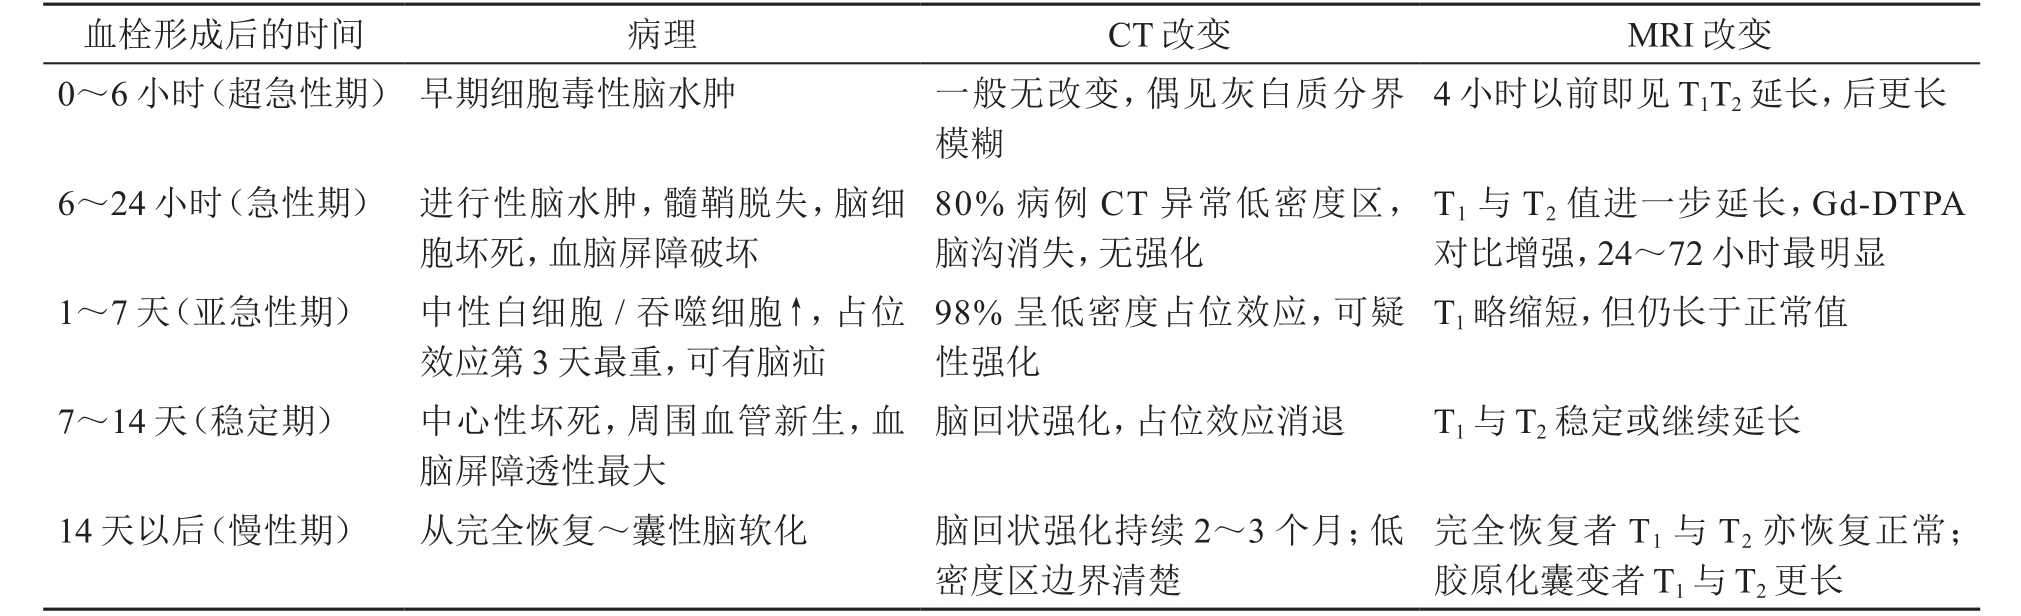
\includegraphics[width=6.72917in,height=2.04167in]{./images/Image00370.jpg}
\end{table}

中年以上的高血压及动脉硬化患者
,静息状态下或睡眠中急性起病,一至数日内出现局灶性脑损害的症状和体征,并能用某一动脉供血区功能损伤来解释,临床应考虑急性脑梗死的可能。CT或MRI检查发现梗死灶可明确诊断。有明显感染或炎症疾病史的年轻患者需考虑动脉炎致血栓形成的可能。

急性缺血性脑卒中诊断流程应包括如下5个步骤:①是否为脑卒中?排除非血管性疾病。②是否为缺血性脑卒中?进行脑CT或MRI检查排除出血性脑卒中。③脑卒中严重程度?根据神经功能缺损量表评估。④能否进行溶栓治疗?核对适应证和禁忌证(见溶栓中相关内容)。⑤病因分型:对急性缺血性脑卒中患者进行病因分型有助于判断预后、指导治疗和选择二级预防措施。当前国际广泛使用TOAST病因分型,将缺血性脑卒中分为:大动脉粥样硬化型、心源性栓塞型、小动脉闭塞型、其他明确病因型和不明确原因型5型。

鉴别诊断方面主要应与以下疾病鉴别:

\paragraph{脑出血、蛛网膜下腔出血和脑栓塞}

其鉴别诊断见表\ref{tab84-2}。就脑栓塞而言,以风心病二尖瓣狭窄伴房颤最为多见,其次是AMI伴房颤,找到栓子的来源是鉴别诊断的重要依据。

\paragraph{颅内占位病变}

脑肿瘤、硬膜下血肿和脑脓肿可呈卒中样发病,出现偏瘫等局灶性体征,颅内压增高征象不明显时易与脑梗死混淆。应详询病史,如硬膜下血肿有许多病例外伤轻微,患者毫无介意或已遗忘,或发病是在外伤数月之后,不追问外伤史,则易误诊。CT或MRI扫描有助确诊。

\paragraph{高血压脑病}

可有偏瘫、偏盲,发病突然、需与脑梗死鉴别。但其常有高血压,可达200/120mmHg以上,降压后神经障碍迅速恢复,眼底可见视乳头水肿、视网膜出血及渗出物。CT或MRI检查可助鉴别。

\subsubsection{脑栓塞}

\hypertarget{text00242.htmlux5cux23CHP8-1-2-2-2-1}{}
(一) 临床表现特点

1.发病年龄
因原发病因而不同,有风心瓣膜病变者以青、中年女性多见;因冠心病、动脉粥样硬化或心肌梗死引起的,以老年人多见。

2.突然起病是其主要特征
。常无任何先兆的突然发病,在数秒或数分钟内症状发展到最高峰,是所有脑血管疾病中发病最快者。多属完全性卒中。活动与安静时均可发病。50\%~60\%的患者起病时有短暂的意识障碍,持续数分钟后随之清醒或呈一过性神志恍惚与精神错乱。9\%~18\%的患者有癫痫发作,一般先是单纯部分性发作,继之发展为全身强直-阵挛发作。少数多发性皮质栓塞可引起癫痫持续状态,预后极差。

3.脑栓塞发病后立即出现的局灶性神经体征,按受累动脉不同而表现为各种脑血管综合征(详见脑血栓形成部分)。大约4/5的脑栓塞累及Willis环的前半部,以大脑中动脉阻塞综合征最常见,表现为对侧中枢性面瘫、偏瘫或单瘫,可伴失语或单纯部分性癫痫发作。偏瘫以对侧下面部与上肢为重,下肢较轻,有时伴轻度感觉障碍。大约l/5的脑栓塞发生在Willis环的后半部,即椎-基底动脉系统,表现为眩晕、皮质盲、复视、眼震、共济失调、交叉性瘫痪或四肢瘫、发音与吞咽困难等。意识障碍有无取决于栓塞血管的大小和梗死的面积。网状结构受累为主者可出现昏迷与高热。延髓生命中枢受损严重者可立即致死。

4.有些患者神经体征迅速好转
,可能因侧支动脉痉挛解除,或栓子溶解破裂而进入了更小的动脉。有些患者逐渐加重,可能因栓塞处继发了血栓形成并向近端蔓延,或由缺血性梗死转为出血性梗死之故。

\begin{table}[htbp]
\centering
\caption{四种急性脑血管病的临床鉴别诊断}
\label{tab84-2}
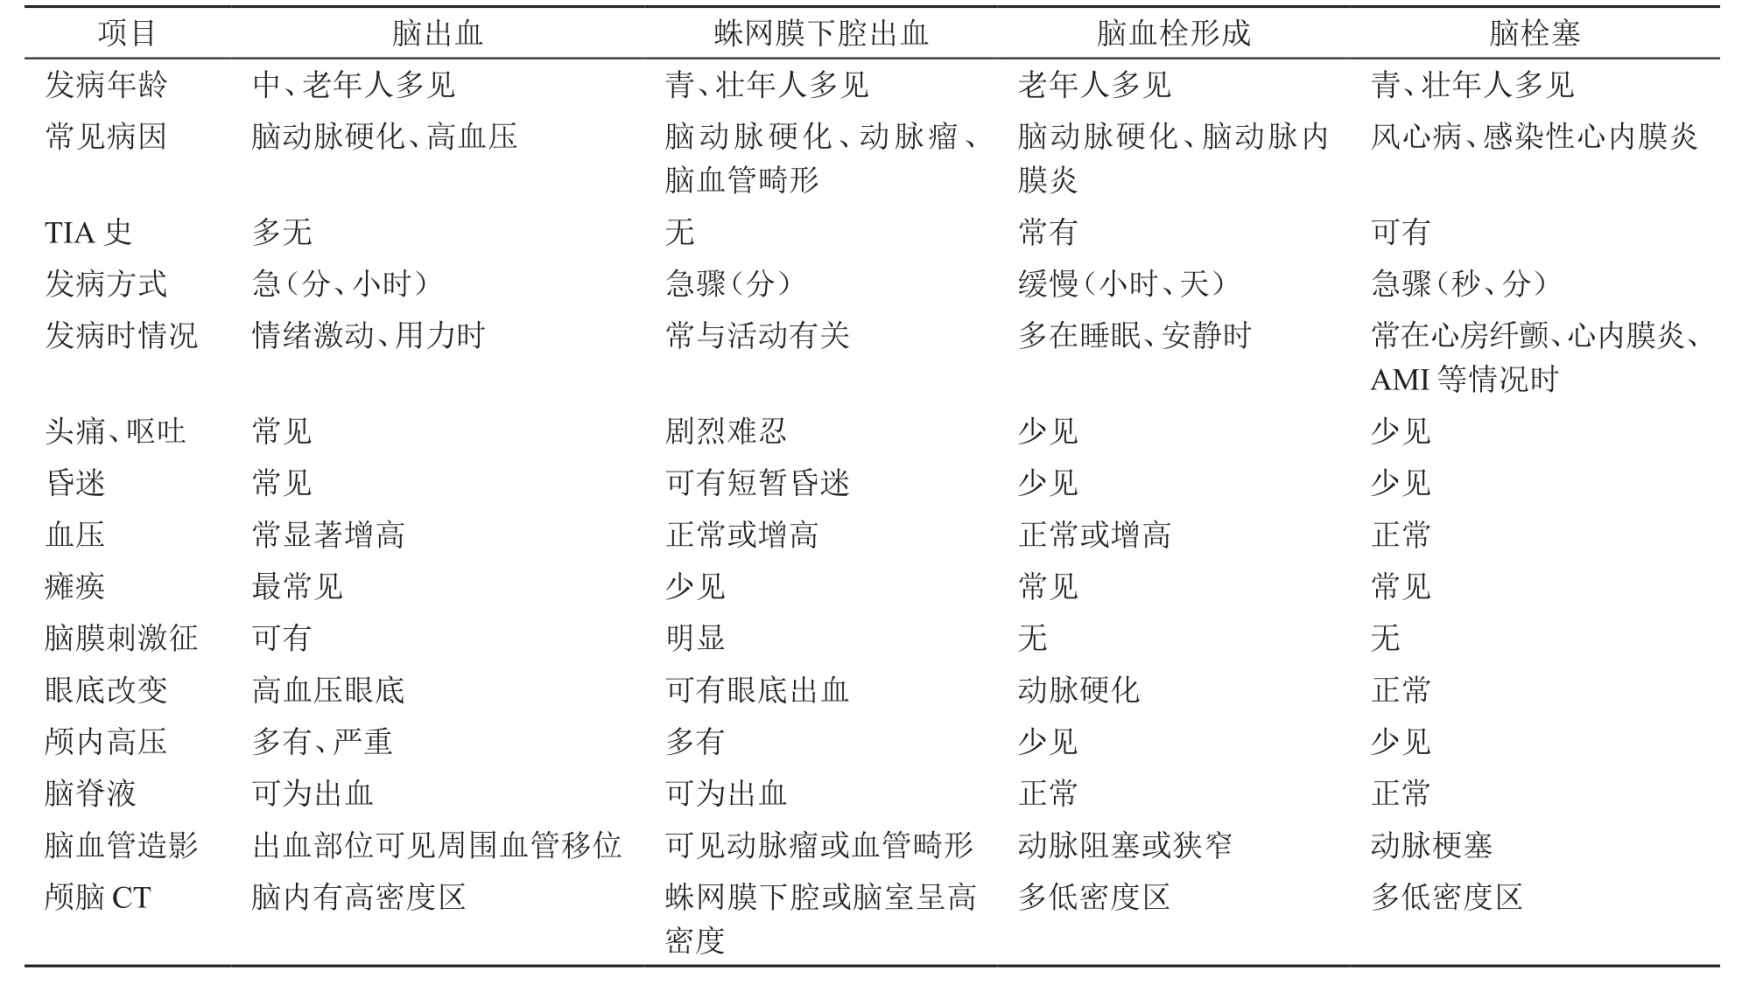
\includegraphics[width=6.625in,height=3.75in]{./images/Image00371.jpg}
\end{table}

5.大多数患者伴有风湿性心脏病、冠心病和严重心律失常等,或存在心脏手术、长骨骨折、血管内介入治疗等栓子来源病史。有些患者同时并发肺栓塞(气急、发绀、胸痛、咯血和胸膜摩擦音等)、肾栓塞(腰痛、血尿等)、肠系膜栓塞(腹痛、便血等)和皮肤栓塞(出血点或瘀斑)等疾病表现。

\hypertarget{text00242.htmlux5cux23CHP8-1-2-2-2-2}{}
(二) 辅助检查

\paragraph{神经影像学检查}

CT和MRI检查可显示缺血性梗死或出血性梗死改变,合并出血性梗死高度支持脑栓塞诊断。MRA可发现颈动脉狭窄程度或闭塞。

\paragraph{脑脊液检查}

外观一般无色透明,可有压力增高,出血性脑梗死者红细胞增加,可达1000 ×
10\textsuperscript{6}
/L,感染性脑梗死者白细胞增加,如非必要尽量避免行此项检查。

\paragraph{其他检查}

心电图应常规检查,作为诊断心肌梗死和心律失常的依据。心脏超声、X线胸片等检查有助于了解心脏情况。如疑有主动脉弓大血管或颈部血管病变时,可作血管超声或脑血管造影。

\hypertarget{text00242.htmlux5cux23CHP8-1-2-2-2-3}{}
(三) 诊断注意事项

根据骤然起病,数秒至数分钟达到高峰,出现偏瘫、失语等局灶性神经功能缺损,既往有栓子来源的基础疾病如心脏病、动脉粥样硬化、严重的骨折等病史,基本可作出临床诊断,如合并其他脏器栓塞更支持诊断。CT和MRI检查可确定脑栓塞部位、数目及是否伴发出血,有助于明确诊断。

脑栓塞主要应与动脉硬化性脑梗死、脑出血、蛛网膜下腔出血鉴别,参见表\ref{tab84-2}。

\subsubsection{出血性脑梗死}

脑梗死后由于缺血区血管再通,在梗死区内有血液溢出,这种现象即为出血性脑梗死(hemorrhagic
infarction,HI),或称为梗死后出血。以发病后第2周最常见。其发生主要是由于动脉阻塞后,阻塞部位以下的动脉麻痹、扩张、血压下降,使栓子走向远端或栓子破碎溶解移向远端,这时在血管壁已有缺血改变的部位因血液循环和血压恢复,血流重灌注,血液可从病变的血管漏出或穿破血管进入脑组织,形成HI。因此,脑梗死后,凡能影响栓子消失、缺血血管的变化和血液再灌注的因素均有促进HI发生的作用。HI多见于心源性脑梗死和大面积血栓形成性脑梗死。早期应用抗凝、溶栓、扩容扩血管以及早期行外科手术、恢复脑灌注均可促发HI。HI除脑梗死本身表现外,其发生后的症状是否恶化取决于继发出血的时间、病灶大小和出血程度,是否应用抗凝、溶栓、扩血管等治疗。以下几条有助于HI的诊断。

1.有已确诊的脑梗死存在。

2.脑梗死的临床表现有加重趋势。

3.CT显示皮质下脑梗死区内有不规则高密度出血灶、梗死区外有斑片状出血灶或脑深部大梗死区内形成血肿。梗死区于第2周内出现强化现象。与原发脑出血(尤当无HI前CT对照时)的鉴别是:高密度影外形不规则、边缘不清、密度较低而不均匀,周围低密度带宽而不规则,出血常位于病灶末端或皮质,占位效应轻微或不存在,出血常不破入脑室,病灶区呈斑点状或脑回状强化影。与肿瘤出血的鉴别是:肿瘤出血常发生于肿瘤囊性变或坏死区内,密度高,常见血液平面,有时还可呈不均的高密度影,增强扫描时肿瘤组织有强化反应。MRI显示出血后血红蛋白演变的MRI特征。

4.脑脊液检查从原先正常变为血性、黄变或镜下有较多红细胞。脑脊液/血清内白蛋白比例超过正常。

5.脑血管造影发现原闭塞血管再通。

HI的治疗与一般脑梗死相同,但应立即停用抗凝药、纤溶药及抗血小板凝集药,采用中性治疗为主。

\subsubsection{腔隙性脑梗死}

腔隙性脑梗死(lacunar infarct)或腔隙卒中(lacunar
stroke)是指大脑半球或脑干深部的小穿通动脉,在长期高血压基础上,血管壁发生病变,最终管腔闭塞,导致缺血性微梗死,缺血、坏死和液化的脑组织由吞噬细胞移走形成空腔,故称腔隙性脑梗死。主要累及脑的深部白质、基底节、丘脑和脑桥等部位,形成腔隙状梗死灶。部分病例的病灶位于脑的相对静区,无明显的神经缺损症状,放射学检查或尸检时才得以证实,故称为静息性梗死或无症状性梗死。腔隙性脑梗死约占全部脑梗死的20\%~30\%。

腔隙性脑梗死的主要病因为高血压导致小动脉及微小动脉壁脂质透明变性,管腔闭塞产生腔隙性病变。舒张压增高对于多发性腔隙性脑梗死的形成更为重要。病变血管多为直径100~200μm的深穿支,如豆纹动脉、丘脑穿通动脉及基底动脉旁中央支,多为终末动脉,侧支循环差。高血压性小动脉硬化引起管腔狭窄时,继发血栓形成或脱落的栓子阻断血流,会导致供血区的梗死。多次发病后脑内可形成多个病灶。

腔隙性梗死灶呈不规则圆形、卵圆形或狭长形,直径在0.2~20mm,多为3~4mm。病灶常位于脑深部核团(壳核约37\%、丘脑14\%、尾状核10\%),脑桥(16\%)和内囊后肢(10\%),内囊前肢和小脑较少发生。

本病多见于中老年患者,男性多于女性,半数以上的病例有高血压病史,突然或逐渐起病,出现偏瘫或偏身感觉障碍等局灶症状。通常症状较轻、体征单一、预后较好,一般无头痛、颅高压和意识障碍表现,许多患者并不出现临床症状而由头颅影像学检查发现。

Fisher等将腔隙性卒中归纳为20余种临床表现形式,但最常见的是以下五型。

\paragraph{纯运动性轻偏瘫(pure motor hemiparesis,PMH)}

病变在内囊、放射冠或脑桥基底部,主要累及锥体束。本型最常见,约占61\%,常于2周内恢复。其主要表现为:①仅有轻偏瘫。对侧面、上下肢同等程度的轻偏瘫,也可以面肌与上肢受累为主,偶见对侧核上性面神经麻痹。②无视野缺损、失语、失用或失认等症。③可有主观感觉异常,但无客观感觉障碍。

\paragraph{纯感觉性卒中(pure sensory stroke,PSS)}

病灶在丘脑腹后外侧核,故感觉障碍严格按正中轴分布。常于数周内恢复,分持续性与短暂性两种。主要表现为:①仅有偏身感觉障碍如对侧面部及肢体感觉障碍;或仅累及面部及肢体某部。②神经功能障碍客观检查常比主观症状轻,自觉麻木、发热、灼热或触觉过敏。③在卒中发作之前大约10\%可有前驱性感觉性TIA症状。

\paragraph{共济失调性轻偏瘫(ataxic hemiparesis,AHP)}

病变在脑桥基底部上中1/3交界处与内囊,或皮质下白质。主要表现为:①对侧肢体共济失调与轻偏瘫,下肢重于上肢;②有时可伴感觉障碍。

\paragraph{构音障碍 -手笨拙综合征(dysarthria-clumsy hand syndrome,DCHS)}

脑桥基底部上中1/3交界处与内囊膝部病灶,均可引起本综合征。主要表现为:①严重构音困难、呐吃,可伴吞咽困难现象。②对侧偏身共济失调,上肢重于下肢,特点是手无力与笨拙,不能做精细动作。③无感觉障碍。④可伴对侧中枢性面瘫、舌瘫与锥体束征。

\paragraph{感觉运动性卒中(sensorimotor stroke,SMS)}

主要表现为:①对侧肢体感觉障碍及轻偏瘫均相当明显;②无意识障碍、记忆力障碍、失语、失用及失认。病灶位于丘脑腹后核及邻近内囊后肢,是丘脑膝状体动脉分支或脉络膜后动脉丘脑支闭塞所致。

腔隙状态(lacunar
state)是本病反复发作引起多发性腔隙性梗死,累及双侧皮质脊髓束和皮质脑干束,出现严重精神障碍、痴呆、假性延髓性麻痹、双侧锥体束征、类帕金森综合征和尿便失禁等。

CT诊断阳性率介于49\%~92\%,扫描以起病后10天~l个月最好。所见的腔隙多位于基底节区(尾状核、内囊、放射冠、豆状核、苍白球),为圆形,边清、质匀的低密度影,直径平均3~13mm。因腔隙性梗死的受累小动脉直径均小于500μm(一般为100~200μm),故脑血管造影不能发现闭塞的血管。脑电图一般无异常表现。然而,MRI显示腔隙性梗死灶远比CT优越,腔隙性梗死显示得早,腔隙灶数目比CT多,定位更准确,还能区别陈旧的腔隙是腔隙性梗死遗留的残腔,还是小灶性脑出血遗留的残腔。

治疗与脑血栓形成治疗类似。主要是控制脑血管病危险因素,尤其要强调积极控制高血压。可以应用抗血小板聚集剂如阿司匹林,也可用钙离子拮抗剂如尼莫地平等治疗,目前没有证据表明抗凝治疗有效。

本病预后一般良好,死亡率和致残率较低,但复发率较高。

\subsubsection{分水岭脑梗死}

分水岭梗死是指脑、心、肾等器官内较大的相邻血管供血区之间的边缘带的一种局部缺血性损害。分水岭脑梗死(cerebral
watershed
infarction,CWSI)是两支主要脑动脉分布区边缘带发生的脑梗死,也称边缘带(border
zone)脑梗死,占全部脑梗死的10\%。严重低血压、心脏骤停等原因引起的分水岭梗死多为双侧性;若一侧脑血管原先即有动脉硬化性狭窄或闭塞性病变,当全身血压过低时其远端小动脉即发生低灌流状态,从而引起单侧分水岭梗死。分水岭梗死以幕上性最多见,主要分为三型:①前分水岭梗死:梗死发生于大脑前动脉与大脑中动脉皮质支的边缘带。其典型症状主要表现为除面部以外的轻偏瘫,尤以下肢明显,半数伴感觉异常。病变在优势半球者会有皮质性运动性失语,表现为重复语言,暴发性短句;非优势半球受损者常伴有情绪改变或精神障碍。②后分水岭梗死位于大脑中动脉与大脑后动脉皮质支的边缘带(最常见)。其典型症状以偏盲最常见,以下象限最明显,伴黄斑回避现象。另外常见皮质性偏身感觉减退,表现为两点辨别觉及形体觉障碍。③皮质下分水岭梗死:梗死位于大脑中动脉皮质支与深穿支的边缘带。其典型症状主要表现为轻偏瘫,半数可有对侧偏身感觉减退,一般为传导束性。优势半球病灶可致不全运动性失语。幕下分水岭梗死(小脑分水岭梗死)较少见,梗死位于小脑主要动脉末端的边缘区。可引起轻度的共济失调。CT示带状略呈楔形低密度区。MRI征象与血栓形成性脑梗死相同。确诊分水岭梗死,还必须结合以下几点:①有引起全身低血压的病史;②梗死区位于大脑前、中动脉交界区,或大脑中、后动脉交界区;③分水岭梗死常为双侧性。其治疗原则同一般脑梗死,由全身低血压所致者必须针对原发性疾病加以处理,尽快纠正低血压状态。

\subsection{治疗}

\subsubsection{治疗原则}

脑梗死的治疗原则:①超早期治疗:强调治疗时间窗概念,争取超早期治疗,力争发病后尽早选用最佳治疗方案,要像对待急性心肌梗死那样来对待缺血性脑卒中,以尽早恢复或改善脑局部缺血区的血液供给,最大限度地争取神经细胞存活,减少细胞死亡,缩小半影区,减少梗死灶面积,降低致残率和病死率。②个体化治疗:根据患者年龄、缺血性卒中类型、病情严重程度和基础疾病等采取最适当的治疗。③整体化治疗:采取针对性治疗同时,进行支持疗法、对症治疗和早期康复治疗,对卒中危险因素如高血压、糖尿病和心脏病等及时采取预防性干预,减少复发率和降低病残率。

2007年
AHA与ASA(美国卒中协会)颁布了“成人缺血性卒中患者的早期处理指南”,2010年年初中华医学会神经病学分会脑血管病学组颁布了“中国急性缺血性脑卒中诊治指南2010”。现结合上述的有关指南,就脑梗死的早期处理简介如下。

\subsubsection{快速评价}

初诊评价的首要目的是证实患者的功能缺损是缺血性卒中所致,而不是其他系统或其他神经系统疾病尤其是颅内出血所致;其次,有助于及时使用溶栓药物做紧急治疗;最后,进行诊断性检查以筛查卒中急性期的内科或神经系统并发症;最后,初诊鉴别能提供病史资料和其他信息以用于确定卒中的血管分布区域,并且提供其可能的病理生理学或病因学线索,以便于作出进一步的合理治疗以预防卒中复发。

\paragraph{院前评估}

院前处理的关键是迅速识别疑似脑卒中患者并尽快送到医院。有关指南将卒中处理的要点总结7个“D”,便于急救医疗人员掌握记忆。即:发现(detection)、派遣(dispatch)、转运(delivery)、入急诊(door)、资料(data)、决策(decision)和药物治疗(drug)。上述每一点上的延误都可引起抢救的耽搁,因此在每一环节的处理都应熟练而准确到位。前3个“D”是由院前急救人员和目击者提供的基本生命支持(BLS)阶段。当患者、家属或现场人员认识到卒中或TIA症状时,可启动急救医疗系统(通过急救电话)。院前急救人员必须对怀疑脑卒中患者提供优先服务及优先转送。院前急救人员必须反应迅速,确定脑卒中的症状和体征,并将患者送至有条件在到达急诊后1小时内开始溶栓治疗的医院。最后3个“D”在院内进行,资料收集包括进行CT扫描(data),对有明确溶栓适应证者作出决策(decision),并进行有效的药物治疗(drug)。

\hypertarget{text00242.htmlux5cux23CHP8-1-2-3-2-1-1}{}
(1) 院前脑卒中的识别:

若患者突然出现以下症状时应考虑脑卒中的可能:①一侧肢体(伴或不伴面部)无力或麻木;②一侧面部麻木或口角歪斜;③说话不清或理解语言困难;④双眼向一侧凝视;⑤一侧或双眼视力丧失或模糊;⑥眩晕伴呕吐;⑦既往少见的严重头痛、呕吐;意识障碍或抽搐。也可采用Cincinnati院前脑卒中评价表(表\ref{tab84-3})进行评估。

\begin{table}[htbp]
\centering
\caption{Cincinnati脑卒中评价表}
\label{tab84-3}
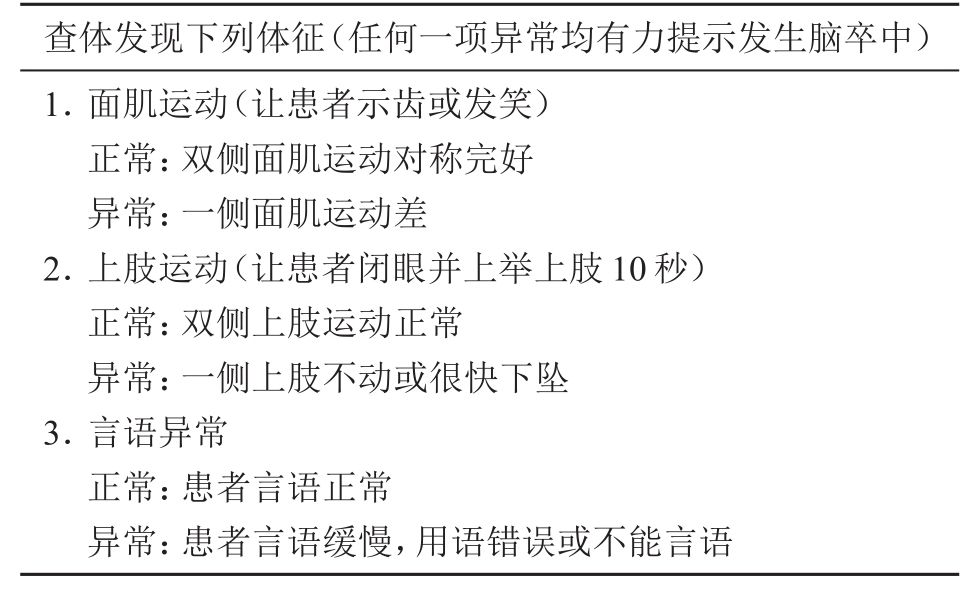
\includegraphics[width=3.25in,height=1.95833in]{./images/Image00372.jpg}
\end{table}

\hypertarget{text00242.htmlux5cux23CHP8-1-2-3-2-1-2}{}
(2) 现场处理及运送:

现场急救人员应尽快进行简要评估和必要的急救处理,包括:①处理气道、呼吸道和循环问题;②心脏观察;③建立静脉通道;④吸氧;⑤评估有无低血糖。应避免:①非低血糖患者输含糖液体;②过度降低血压;③大量静脉输液。应迅速获取简要病史,包括:①症状开始时间;②近期患病史;③既往病史;④近期服药史。应尽快将患者送至附近有条件的医院(能24小时进行急诊CT检查)。并在到达之前通知医院内进行人员设备准备,以确保快速院内评估处理的顺利进行,并在治疗时间窗内判断是否适宜溶栓治疗。

\paragraph{院内(急诊室)评估}

由于急性缺血性脑卒中的治疗时间窗窄,及时评估病情和诊断至关重要,医院应建立脑卒中诊治快速通道,尽可能优先处理和收治脑卒中患者。

\hypertarget{text00242.htmlux5cux23CHP8-1-2-3-2-2-1}{}
(1) 诊断和评估内容:

病史采集和体格检查:疑似脑卒中患者到达医院后,尽快进行病史采集和体格检查,并评估:①是否为脑卒中?注意发病形式、发病时间,排除脑外伤、中毒、癫痫后状态、脑卒中、高血压脑病、血糖异常、脑炎及躯体重要脏器功能严重障碍等引起的脑部病变。进行必要的实验室检查。②是缺血性还是出血性脑卒中?除非特殊原因不能检查,所有疑为脑卒中患者都应尽快进行脑影像学(CT或MRI)检查,排除出血性脑卒中、确立缺血性脑卒中的诊断。③是否适合溶栓治疗?发病时间是否在4.5小时或6小时内,有无溶栓适应证。尽可能在到达急诊室后60分钟内完成脑CT等评估并作出治疗决定。

获取病史以及进行全面的内科和神经系统体格检查能迅速为急诊的鉴别诊断提供依据。有选择的诊断性检查能为临床鉴别提供辅助依据。卒中患者通常有突发或者急性发作的局灶性神经系统症状的病史。临床医生根据缺血性卒中患者常见的神经系统异常表现(表\ref{tab84-4})对卒中的诊断准确性是较高的,经常混淆的诊断包括未被发现的癫痫发作、意识模糊状态、晕厥、中毒或代谢性疾病(包括低血糖)、颅内肿瘤及硬膜下血肿等,但这些类似卒中表现的疾病通常累及全身而不仅仅只有神经系统症状,且常常能通过辅助检查(见前述)而迅速鉴别。脑成像检查(CT或MRI等)对鉴别缺血性卒中和出血性卒中或其他可能类似卒中的大脑结构损害是必需的。

\begin{table}[htbp]
\centering
\caption{缺血性卒中患者常见的神经系统异常表现}
\label{tab84-4}
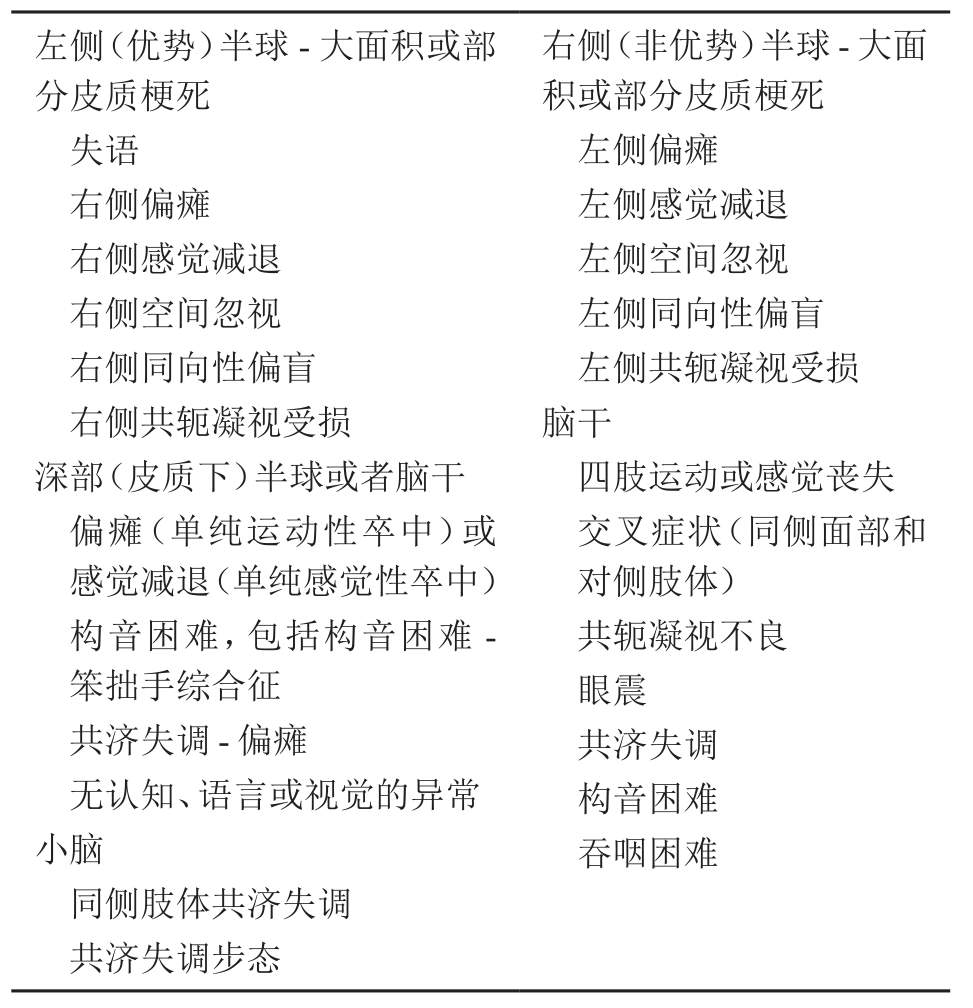
\includegraphics[width=3.23958in,height=3.35417in]{./images/Image00373.jpg}
\end{table}

当考虑使用溶栓药物时,症状的起始时间是最关键的。起始时间定为患者被确认无症状的最后时间。因为缺血性卒中经常不伴有疼痛,多数患者没有被疾病发作所惊醒。因此,若患者在唤醒的时候有卒中症状,那么起始时间就定为患者在就寝前最后被确知无症状的时间。若患者开始时症状轻微,在随后数小时内症状加重,那么症状首先出现的时间被定为起始时间。若患者的症状完全缓解以后(TIA),接着发生第二个事件,那么新症状的出现时间被定为起始时间。

根据神经系统检查来判定卒中的严重程度是一个有力的诊断指示指标。目前广泛应用的是美国国立卫生研究院卒中量表(NIHSS)(表\ref{tab84-5})。NIHSS初评得分能提供重要的诊断信息。大约60\%~70\%基础NIHSS得分<
10分的缺血性卒中患者在1年以后仍预后良好;基础NIHSS得分>
20分的患者仅有4\%~16\%在1年后仍预后良好。同时NIHSS得分有助于鉴别那些溶栓治疗中存在很大颅内出血风险的患者。在rtPA的NINDS试验中,那些NIHSS得分达到或超过20分的患者,颅内出血率约17\%,而得分<
10分的患者出血率仅为3\%。

对于需进行溶栓治疗的缺血性卒中患者,美国国立神经病与卒中学会(NINDS)提出的患者在医院内各种检查所需的最多时间见表\ref{tab84-6}。

\begin{table}[htbp]
\centering
\caption{国立卫生研究院卒中量表(NIHSS)}
\label{tab84-5}
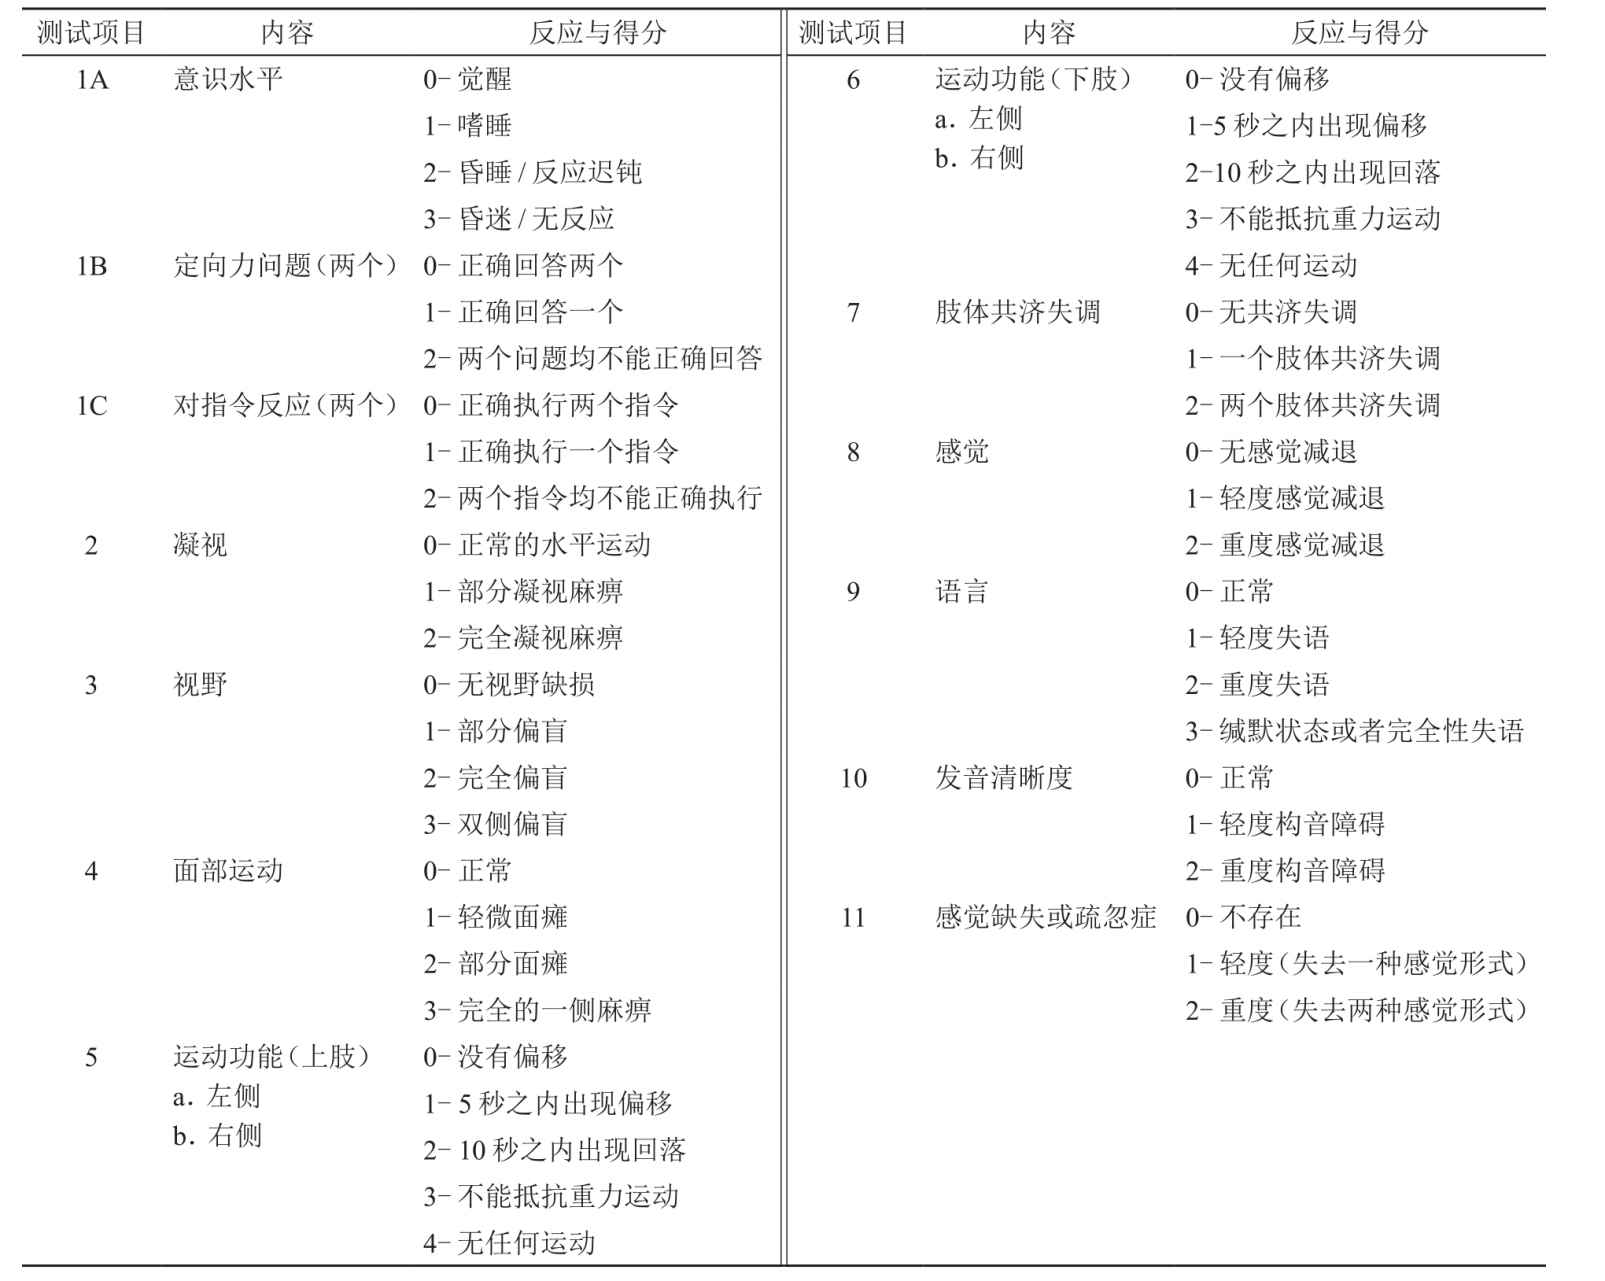
\includegraphics[width=6.79167in,height=5.41667in]{./images/Image00374.jpg}
\end{table}

\begin{table}[htbp]
\centering
\caption{NINDS溶栓治疗患者脑卒中评估表}
\label{tab84-6}
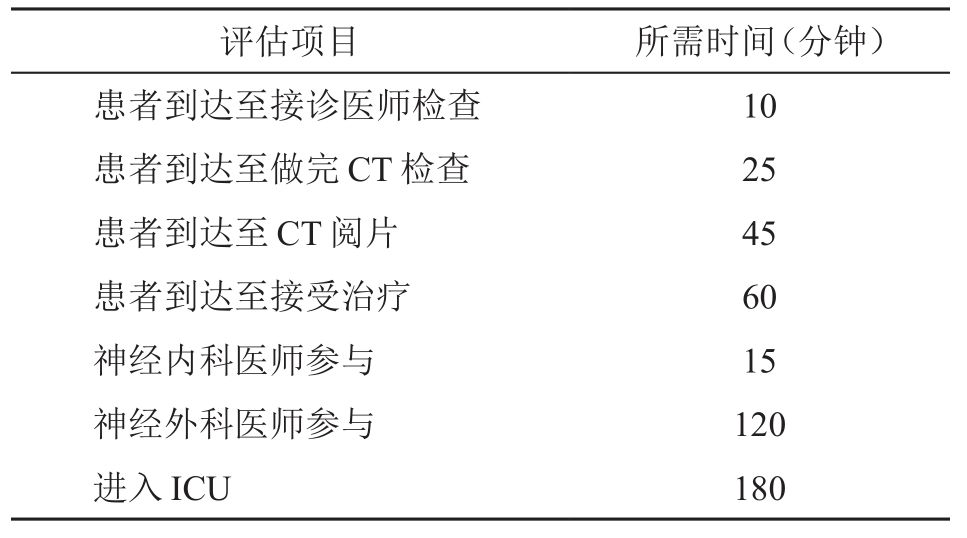
\includegraphics[width=3.20833in,height=1.78125in]{./images/Image00375.jpg}
\end{table}

\hypertarget{text00242.htmlux5cux23CHP8-1-2-3-2-2-2}{}
(2) 急诊室的处理:

在评估的同时,应密切监护基本生命功能,如气道和呼吸;心脏监测和心脏病变处理;血压和体温调控。需紧急处理的情况:颅内压增高、严重血压异常、血糖异常和体温异常、癫痫等(见下述)。

\subsubsection{一般支持性治疗和并发症的处理}

脑梗死患者一般应在卒中单元(stroke
unit,SU)中接受治疗。SU由多科医师、护士和治疗师参与,实施治疗、护理和康复一体化的原则,以最大程度地提高治疗效果和改善预后。中、重度脑卒中,如大面积脑梗死、小脑梗死、椎基底动脉主干梗死及病情不稳定脑梗死患者均应进入SU治疗。欧洲的几项研究证实,SU可以降低卒中死亡率,其益处可与静脉应用rtPA相比。

\paragraph{一般护理观察}

入院后最初24小时内应经常评估患者神经系统状态和生命体征,多数患者应卧床休息,一旦病情稳定就开始活动。在转换成坐住或站位时应密切观察神经系统症状是否加重。瘫痪肢体关节充分的被动活动在最初的24小时内就可以开始。经常翻身,使用压力可变的坐垫,密切监测皮肤等都是重要的内容。早期活动的益处在于预防肺炎、深静脉血栓、压疮等并发症,还可以减少静止不动所导致的痉挛、畸形和压迫性麻痹。

\paragraph{保持气道通畅及供氧}

维持足够的组织供氧在大脑缺血急性期是非常重要的,可防止低氧血症和加重神经系统损伤。低氧血症最常见的病因是部分气道梗阻、低通气、吸入性肺炎或者肺不张。意识水平逐渐下降或者脑干卒中患者因为口咽部运动功能受损而且保护性反射消失,气道受累的危险性增加。因此,昏迷患者应将头歪向一侧,以利于口腔分泌物及呕吐物流出,并可防止舌根后坠阻塞呼吸道。应进行SaO\textsubscript{2}
监测,使其≥95\%。合并低氧血症患者(SaO\textsubscript{2} <
92\%或血气分析提示缺氧)应给予吸氧,气道功能严重障碍者应给予气道支持(气管插管或切开)及辅助呼吸。无低氧血症的患者不需要常规吸氧。

\paragraph{饮食与营养支持}

脑卒中后由于呕吐、吞咽困难可引起脱水及营养不良,可导致神经功能恢复减慢。应重视脑卒中后液体及营养状态评估,必要时给予补液和营养支持。吞咽障碍增加卒中死亡率,故在允许患者进食或饮水之前应评估吞咽能力。吞咽后湿声、口唇闭合不全、NIHSS计分增高都是误吸入危险的独立指征,床边水吞咽试验是有用的筛查试验。正常经口进食者无需额外补充营养。若有吞咽障碍,可插入鼻胃管或鼻十二指肠管以供喂食并便于给药;持续时间长者经本人或家人同意可行经皮内镜下胃造瘘(PEG)管饲补充营养。

\paragraph{血糖控制}

脑卒中急性期高血糖较常见,可以是原有糖尿病的表现或应急反应。应常规检查血糖,当血糖超过11.1mmol/L(200mg/dl)时应立即给予胰岛素治疗,将血糖控制在8.3mmol/L(150mg/dl)以下。开始使用胰岛素时应1~2小时监测血糖一次。脑卒中后低血糖发生率较低,但因低血糖可直接导致脑缺血损伤和水肿加重,对预后不利,故应尽快纠正低血糖。血糖低于2.8mmol/L(50mg/dl)时给予10\%~20\%葡萄糖口服或注射治疗。

\paragraph{血压控制}

约70\%的缺血性脑卒中患者急性期血压升高,原因主要包括:疼痛、恶心呕吐、颅内压增高、意识模糊、焦虑、脑卒中后应激状态、病前存在高血压等。多数患者在脑卒中后24小时内血压自发降低。病情稳定而无颅内高压或其他严重并发症的患者,24小时后血压水平基本可反映其病前水平。缺血性脑卒中后24小时内血压升高的患者应谨慎处理。应先处理紧张焦虑、疼痛、恶心呕吐及颅内压增高等情况。血压持续升高,收缩压≥200mmHg或舒张压≥100mmHg,或伴有严重心功能不全、主动脉夹层、高血压脑病、急性肾衰、急性心肌梗死等,可予谨慎降压治疗,并严密观察血压变化,必要时可静脉使用作用时间短和对脑血管影响较小的药物(如拉贝洛尔、尼卡地平等),最好应用微量输液泵,避免血压降得过低。过度降低血压是有害的,因其可继发缺血区域灌注减少而扩大梗死的范围。应避免舌下含服钙拮抗剂如硝苯地平,因其吸收很快,易继发突然的血压下降。其他能使血压迅速下降的药物也应避免使用。口服药物可选用卡托普利或尼卡地平。准备溶栓治疗的患者血压应控制在收缩压<
180mmHg或舒张压<
100mmHg水平。有高血压病史且正在服用降压药物者,如病情稳定,可于脑卒中24小时后开始恢复使用降压药物。

在急性缺血性卒中患者中,持续性低血压非常少见,但若存在,则必须查明原因。其原因包括主动脉瓣断裂、低血容量和继发于心肌缺血或心律失常的心输出量减少。在卒中后最初数小时内,应纠正血容量不足和使心输出量达到理想目标。治疗措施包括输注生理盐水补充血容量和纠正心律失常,如快速房颤应减慢心室率。若这些措施无效,可应用多巴胺等升压药物,以确保收缩压≥90mmHg。

\paragraph{控制脑水肿、降低颅内压}

急性脑梗死中颅内压增高并不常见。大脑中动脉主干、颈内动脉梗死者可产生急性颅内压增高,但几乎所有的脑梗死患者均有脑水肿,且以发病后3~5天最明显。严重脑水肿和颅内压增高是急性重症脑梗死的常见并发症,是死亡的主要原因。处理脑水肿的目的是:①降低颅内压;②维持适当的脑灌注,避免脑缺血加重;③预防脑疝形成引起继发性脑损伤。目前认为将颅内压(ICP)控制在20mmHg以内,并使脑灌注压(CPP)维持在70mmHg以上最为理想。治疗方法包括:①卧床,避免和处理引起颅内压增高的因素,如头颈部过度扭曲、激动、用力、发热、癫痫、呼吸道不通畅、咳嗽、便秘等(Ⅰ级推荐)。②可使用甘露醇静脉滴注(Ⅰ级推荐,C级证据);必要时也可用甘油果糖或呋塞米等(Ⅱ级推荐,B级证据)。常用的脱水剂如甘露醇、甘油、呋塞米、白蛋白、β-七叶皂苷钠等的具体用法,参见本书第41章“颅高压危象”部分。③对于发病48小时内,60岁以下的恶性大脑中动脉梗死伴严重颅内压增高、内科治疗不满意且无禁忌证者,可请脑外科会诊考虑是否行减压术(Ⅰ推荐,A级证据)。④对压迫脑干的大面积小脑梗死患者可请脑外科会诊协助处理(Ⅲ推荐,C级证据)。

\paragraph{防治心血管并发症}

心肌梗死和心律失常是急性脑梗死潜在的并发症。右侧半球梗死的患者出现心律失常的危险性更高,可能是由于交感和副交感神经系统功能紊乱所致。继发于卒中的心电图改变包括ST段压低、QT间期延长、T波倒置和明显的U波。卒中患者最常见的心律失常是房颤;心肌梗死是与儿茶酚胺释放有关的潜在并发症。因此,脑梗死后24小时内应常规进行心电图检查,必要时进行心电监护,以便早期发现心脏病变并进行相应处理;避免或慎用增加心脏负荷的药物。

\paragraph{防治感染}

脑卒中患者(尤其存在意识障碍者)急性期容易发生呼吸道、泌尿系统感染等,是导致病情加重的重要原因。

\hypertarget{text00242.htmlux5cux23CHP8-1-2-3-3-8-1}{}
(1) 防治肺炎:

约5.6\%脑卒中患者合并肺炎,误吸是主要原因。意识障碍、吞咽困难是导致误吸的主要危险因素,其他包括呕吐、不活动等。肺炎是脑卒中患者死亡的主要原因之一,15\%~25\%脑卒中患者死于细菌性肺炎。措施:①早期评估和处理吞咽困难和误吸问题,对意识障碍患者应特别注意预防肺炎(Ⅰ推荐,C级证据)。患者采用适当的体位,经常翻身叩背及防止误吸是预防肺炎的重要措施。②疑有肺炎的发热患者应给予抗生素治疗,但不推荐预防性使用抗生素(Ⅱ级推荐,B级证据)。

\hypertarget{text00242.htmlux5cux23CHP8-1-2-3-3-8-2}{}
(2) 防治尿路感染:

排尿障碍在脑卒中早期很常见,主要包括尿失禁与尿潴留。住院期间40\%~60\%中重度脑卒中患者发生尿失禁,29\%发生尿潴留。尿路感染主要继发于因尿失禁或尿潴留留置导尿管的患者,约5\%出现脓毒症,与脑卒中预后不良有关。措施:①对排尿障碍进行早期评估和康复治疗,记录排尿日记(Ⅱ推荐,B级证据)。②尿失禁者应尽量避免留置导尿管,可定时使用便盆或便壶,白天每2小时1次,晚上每4小时1次(Ⅰ级推荐,C级证据)。③尿潴留者应测定膀胱残余尿,排尿时可在耻骨上施压加强排尿。必要时可间歇性导尿或留置导尿(Ⅳ推荐,D级证据)。④有尿路感染者应给予抗生素治疗,但不推荐预防性使用抗生素(Ⅰ级推荐)。

此外,对卒中后的发热,除积极查找原因外,并需使用降温措施,包括解热药物治疗和降温设备。降低快速升高的体温可以改善严重患者的预后。低温对于广泛或局部缺氧性脑损伤有神经保护作用。参见本书第25章“急性脑功能衰竭”部分。

\paragraph{防治深静脉血栓形成(DVT)和肺栓塞(PE)}

PE约占卒中患者死亡原因的10\%,在卒中患者中发生率约1\%,症状性DVT发生率为2\%。高龄、静止不动、下肢瘫痪、心房颤动等是DVT和PE危险性增加的原因。防治措施:①鼓励患者尽早活动(包括肢体的被动运动)、抬高下肢;尽量避免下肢(尤其是瘫痪侧)静脉输液(Ⅰ级推荐)。②对于发生DVT及PE高风险且无禁忌证者,可给予低分子肝素和普通肝素,有抗凝禁忌者给予阿司匹林治疗(Ⅰ级推荐,A级证据)。③可联合加压治疗(长筒袜或交替式压迫装置)和药物预防DVT,不推荐常规单独使用加压但对有抗拴禁忌的缺血性脑卒中患者,推荐单独应用加压治疗预防DVT和PE(Ⅰ级推荐,A级证据)。④对无抗凝和溶栓禁忌的DVT或PE患者,首先建议肝素抗凝治疗,症状无缓解的近端DVT或肺栓塞患者可给予溶栓治疗(Ⅳ级推荐,D级证据)。有关抗凝和溶栓治疗的药物与用法参见第100章“肺栓塞”。

\paragraph{防治癫痫}

缺血性脑卒中后癫痫的早期发生率为2\%~33\%,晚期发生率为3\%~67\%。防治措施:①不推荐预防性应用抗癫痫药物。②孤立发作1次或急性期痫性发作控制后,不建议长期使用抗癫痫药物。③脑卒中后2~3个月再发的癫痫,建议按癫痫常规治疗(Ⅰ级推荐)。④脑卒中后癫痫持续状态,建议按癫痫持续状态治疗原则处理(Ⅰ级推荐)。有关癫痫痫性发作及癫痫持续状态的治疗详见第85章“癫痫与癫痫持续状态”。

\paragraph{防治上消化道出血}

高龄和重症脑卒中患者急性期容易发生应激性溃疡,建议常规应用静脉抗溃疡药(H\textsubscript{2}
-RA,或PPI);对已发生上消化道出血患者,则按上消化道出血治疗。详见第13章第1节“上消化道出血”。

\paragraph{防治水电解质平衡紊乱}

脑卒中时由于神经内分泌功能紊乱、进食减少、呕吐及脱水治疗,常并发水电解质平衡紊乱,主要有低钾血症、低钠血症和高钠血症。应对脑卒中患者常规进行水电解质监测并加以纠正。纠正低钠血症和高钠血症均不宜过快,防止脑桥中央髓鞘溶解症和加重脑水肿。

\paragraph{出血转化的处理}

脑梗死出血转化发生率为8.5\%~30\%,其中有症状的为1.5\%~5\%。心源性脑栓塞、大面积脑梗死、占位效应、早期低密度征、年龄大于70岁、应用抗栓药物(尤其是抗凝药物)或溶栓药物等会增加出血转化的风险。研究显示无症状性出血转化的预后与无出血转化相比差异并无统计学意义,目前对无症状性出血转化者尚无特殊治疗建议。对症状性出血转化:①停用抗栓治疗等致出血药物;与抗凝和溶栓相关的出血处理参见有关章节。②何时开始抗凝和抗血小板治疗:对需要抗栓治疗的患者,可于出血转化病情稳定后7~10天开始抗栓治疗;对于再发血栓风险相对较低或全身情况较差者,可用抗血小板药物代替华法林。

\subsubsection{特异性治疗}

特异性治疗指针对缺血损伤病理生理机制中某一特定环节进行的干预。近年研究热点为改善脑血液循环的多种措施(如溶栓、抗血小板、抗凝、抗纤、扩容等方法)及神经保护的多种药物。

\hypertarget{text00242.htmlux5cux23CHP8-1-2-3-4-1}{}
(一) 溶栓治疗

溶栓治疗是目前最重要的恢复血流措施
,重组组织型纤溶酶原激活剂(rtPA)和尿激酶(UK)是我国目前使用的主要溶栓药,溶栓的方法有静脉溶栓和动脉溶栓。目前认为有效抢救缺血半暗带组织的时间窗为4.5小时内或6小时内。

\paragraph{静脉溶栓治疗}

\hypertarget{text00242.htmlux5cux23CHP8-1-2-3-4-1-1-1}{}
(1) 适应证:

①年龄18~80岁;②发病4.5小时内(rtPA)或6小时内(尿激酶);③脑功能损害的体征持续存在超过1小时,且比较严重;④脑CT已排除颅内出血,且无早期大面积脑梗死影像学改变;⑤患者或家属签署知情同意书。

\hypertarget{text00242.htmlux5cux23CHP8-1-2-3-4-1-1-2}{}
(2) 禁忌证:

①既往有颅内出血,包括可疑蛛网膜下腔出血;近3个月有头颅外伤史;近3周内有胃肠或泌尿系统出血;近2周内进行过大的外科手术;近1周内有在不易压迫止血部位的动脉穿刺。②近3个月内有脑梗死或心肌梗死史,但不包括陈旧小腔隙梗死而未遗留神经功能体征。③严重心、肝、肾功能不全或严重糖尿病患者。④体检发现有活动性出血或外伤(如骨折)的证据。⑤已口服抗凝药,且INR大于1.5;48小时内接收过肝素治疗(APTT超出正常范围)。⑥血小板计数低于100
× 10\textsuperscript{9} /L,血糖< 2.7mmol/L。⑦血压:收缩压>
180mmHg,或舒张压> 100mmHg。⑧妊娠。⑨不合作。

\hypertarget{text00242.htmlux5cux23CHP8-1-2-3-4-1-1-3}{}
(3) 用法:

①rtPA
0.9mg/kg(最大剂量90mg)静脉滴注,其中10\%在最初1分钟内静脉推注,其余持续滴注1小时。国内习惯用5mg静注,余45mg
1小时静滴,总量50mg。②尿激酶100万~150万IU,溶于生理盐水100~200ml,持续静脉滴注30分钟。

\hypertarget{text00242.htmlux5cux23CHP8-1-2-3-4-1-1-4}{}
(4) 静脉溶栓的监护及处理:

①尽可能将患者收入重症监护病房或卒中单元进行监护;②定期进行神经功能评估,第1小时内30分钟1次,以后每小时1次,直至24小时;③如出现严重头痛、高血压、恶心或呕吐,应立即停用溶栓药物并行脑CT检查;④定期监测血压,最初2小时内15分钟1次,随后6小时内30分钟1次,以后每小时1次,直至24小时;⑤如收缩压≥180mmHg或舒张压≥100mmHg,应增加血压监测次数,并给予降压药物;⑥鼻饲管、导尿管及动脉内测压管应延迟安置;⑦给予抗凝药、抗血小板药物前应复查颅脑CT。

\hypertarget{text00242.htmlux5cux23CHP8-1-2-3-4-1-1-5}{}
(5) 静脉溶栓的并发症:

①梗死灶继发性出血或身体其他部位出血;②致命性再灌注损伤和脑水肿;③溶栓后再闭塞。

\paragraph{动脉溶栓}

动脉溶栓使溶栓药物直接到达血栓局部,理论上血管再通率应该高于静脉溶栓,且出血风险降低。然而其益处可能被溶栓启动时间的延迟所抵消。作为卒中紧急治疗,可在DSA直视下进行超选择性介入动脉溶栓。需指出的是,进行动脉内溶栓对设备和医师的专业知识的要求较高,因此,患者应在有经验的脑卒中治疗中心接受动脉内溶栓治疗,以便在必要时能立即进行脑血管影像学和介入性神经放射学检查。因此:①发病6小时内由大脑中动脉闭塞导致的严重脑卒中且不适合静脉溶栓的患者,经过严格选择后可在有条件的医院进行动脉溶栓(Ⅱ级推荐,B级证据);②发病24小时内由后循环动脉闭塞导致的严重脑卒中且不适合静脉溶栓的患者,经过严格选择后可在有条件的单位进行动脉溶栓(Ⅲ级推荐,C级证据)。接受动脉内溶栓治疗的患者,仍有接受rtPA静脉内溶栓治疗的可能性。

有关动脉溶栓的适应证、禁忌证及并发症与静脉溶栓基本相同。

\hypertarget{text00242.htmlux5cux23CHP8-1-2-3-4-2}{}
(二) 抗血小板治疗

常用的抗血小板聚集剂包括阿司匹林和氯吡格雷。建议:①抗血小板药物的选择以单药治疗为主,氯吡格雷、阿司匹林都可以作为首选药物(Ⅰ级推荐,A级证据);有证据表明氯吡格雷优于阿司匹林,尤其对于高危患者获益更显著(Ⅰ级推荐,A级证据);②对于不符合溶栓适应证且无禁忌证的缺血性脑卒中患者应在发病后尽早给予口服阿司匹林150~300mg/d(Ⅰ级推荐,A级证据)。急性期后可改为预防剂量(50~150mg/d);③溶栓治疗者,阿司匹林等抗血小板药物应在溶栓24小时后开始使用(Ⅰ级推荐,B级证据);④对不能耐受阿司匹林者,可考虑选有氯吡格雷(75mg/d)等抗血小板治疗(Ⅲ级推荐,C级证据);⑤不推荐常规应用双重抗血小板药物(Ⅰ级推荐,A级证据)。但对于有急性冠状动脉疾病(例如不稳定型心绞痛,无Q波心肌梗死)或近期有支架成形术的患者,推荐联合应用氯吡格雷和阿司匹林(Ⅰ级推荐,A级证据)。

\hypertarget{text00242.htmlux5cux23CHP8-1-2-3-4-3}{}
(三) 抗凝治疗

急性期抗凝治疗虽然已应用 50多年
,但一直存在争议。Cochrane系统评价纳入24个RCT共23
748例患者,药物包括普通肝素、低分子肝素、类肝素、口服抗凝剂和凝血酶抑制剂。其Meta分析显示:抗凝药治疗不能降低随访期末病死率;随访期末的残疾率亦无明显下降;抗凝治疗能降低缺血性脑卒中的复发率、降低肺栓塞和深静脉血栓形成发生率,但被症状性颅内出血增加所抵消。心脏或动脉内血栓、动脉夹层和椎-基底动脉梗死等特殊亚群尚无证据显示抗凝的净疗效。因此:①对大多数急性缺血性脑卒中患者,不推荐无选择性的早期进行抗凝治疗(Ⅰ级推荐,A级证据);②关于少数特殊患者(如主动脉弓粥样硬化斑块、基底动脉梭形动脉瘤、颈动脉夹层、卵圆孔未闭伴深静脉血栓形成或房间隔瘤等)的抗凝治疗,可在谨慎评估风险、效益比后慎重选择(Ⅳ级推荐,D级证据);③特殊情况下溶栓后还需抗凝治疗的患者,应在24小时后使用抗凝剂(Ⅰ级推荐,B级证据)。

抗凝药物的应用方法参见本章第1节“短暂性脑缺血发作”部分。

\hypertarget{text00242.htmlux5cux23CHP8-1-2-3-4-4}{}
(四) 降纤治疗

很多研究显示脑梗死急性期血浆纤维蛋白原和血液黏滞度增高
,蛇毒酶制剂可显著降低血浆纤维蛋白原,并有轻度溶栓和抑制血栓形成的作用。因此,对不适合溶栓并经过严格筛选的脑梗死患者,特别是高纤维蛋白血症者可选用降纤治疗(Ⅱ级推荐,B级证据)。可选择的药物包括巴曲酶(batroxobin)、降纤酶(defibrase)、安克洛酶(ancrod)和蚓激酶等。巴曲酶首剂10BU,以后隔日5BU,静脉注射,共3~4次。用药过程中监测纤维蛋白原,防止出血的发生。

\hypertarget{text00242.htmlux5cux23CHP8-1-2-3-4-5}{}
(五) 扩容治疗

对一般缺血性脑卒中患者,目前尚无充分RCT支持扩容升压可改善预后。Cochrane系统评价(纳入18项RCT)显示,脑卒中后早期血液稀释疗法有降低肺栓塞和下肢深静脉血栓形成的趋势,但对近期或远期病死率及功能结局均无显著影响。因此:①对一般缺血性脑卒中患者,不推荐扩容(Ⅱ级推荐,B级证据);②对于低血压或脑血流低灌注所致的急性脑梗死如分水岭梗死可考虑扩容治疗,但应注意可能加重脑水肿、心功能衰竭等并发症。此类患者不推荐使用扩血管治疗(Ⅲ级推荐,C级证据)。常用制剂为低分子右旋糖酐,500ml静滴,每日1次,10~14天为一疗程。

\hypertarget{text00242.htmlux5cux23CHP8-1-2-3-4-6}{}
(六) 扩张血管治疗

目前缺乏血管扩张剂能改善缺血性脑卒中临床预后的大样本高质量
RCT证据,因此,对一般缺血性脑卒中患者,不推荐扩血管治疗(Ⅱ级推荐,B级证据)。

\hypertarget{text00242.htmlux5cux23CHP8-1-2-3-4-7}{}
(七) 神经保护剂

理论上
,针对急性缺血或再灌注后细胞损伤的药物(神经保护剂)可保护脑细胞,提高对缺血缺氧的耐受性。但大多数神经保护剂包括自由基清除剂、电压门控性钙通道阻滞剂、兴奋性氨基酸受体阻断剂、阿片受体阻断剂和镁制剂等,在动物试验中的疗效未能得到临床试验的肯定。因此,神经保护剂的疗效和安全性尚需开展更多高质量临床试验进一步证实(Ⅰ级推荐,B级证据)。有关脑保护剂的种类与使用方法,详见本书第25章“急性脑功能衰竭”治疗部分。

\hypertarget{text00242.htmlux5cux23CHP8-1-2-3-4-8}{}
(八) 其他疗法

1.丁苯酞
丁苯酞是近年国内开发的Ⅰ类新药。实验研究表明,本品可阻断缺血性脑卒中所致脑损伤的多个病理环节,具有较强的抗脑缺血作用,明显缩小局部脑缺血的梗死面积,减轻脑水肿,改善脑代谢和缺血脑区的微循环和血流量,抑制神经细胞凋亡,并具有抗脑血栓形成和抗血小板聚集作用。几项评价急性脑梗死患者口服丁苯酞的多中心随机、双盲、安慰剂对照试验显示:丁苯酞治疗组神经功能缺损和生活能力评分均较安慰剂对照组显著改善,安全性好。用法:成人0.2g口服,3次/天,10天为一疗程;静脉滴注:25mg/次,2次/天,疗程14天。本品应在发病后48小时内开始给药。

2.人尿激肽原酶
人尿激肽原酶(尤瑞克林)是近年国内开发的另一个Ⅰ类新药。本品有两点突出于其他药物的作用:①在临床剂量下,选择性扩张缺血部位细小动脉,改善梗死灶内供血,对一般动脉影响不大(不扩张正常动脉,不引起缺血区盗血);②促进损伤部位新生血管的生成。此外,尚具有改善红细胞变形能力和氧解离能力、促进组织对葡萄糖的利用、抑制血小板聚集等作用。评价急性脑梗死患者静脉使用人尿激肽原酶的多中心随机、双盲、安慰剂对照试验显示:尤瑞克林治疗组的功能结局较安慰剂组明显改善并安全。

3.高压氧和亚低温的疗效和安全性还需开展高质量的RCT证实。

\subsubsection{中医中药}

中成药在我国广泛用于治疗缺血性脑卒中已有多年。一项系统评价共纳入191项临床试验,涉及21种中成药共189项临床试验(19
180例患者)的Meta分析显示其能改善神经功能缺损,但得进一步开展高质量研究予以证实。常用的中成药有:①清开灵注射液:20~40ml加入液体静滴,每日1次;②丹参注射液:10~20ml加入液体静滴,每日1次;③川芎嗪注射液:80~120mg加入250~500ml液体中静滴,每日1次;④灯盏花素注射液:20~30ml加入液体静滴,每日1次;⑤脉络宁注射液:10~20ml加入250~500ml液体中静滴,每日1次;⑥血塞通注射液:200~400mg加入液体静滴,每日1次;⑦醒脑静注射液:5~10ml加入250~500ml液体静滴,每日1次;⑧银杏达莫注射液:240mg加入液体静滴,每日1次。上述中成药注射液疗程一般10天左右。

\subsubsection{外科治疗}

\paragraph{颈动脉内膜剥脱术(carotid endarterectomy,CEA)}

根据北美症状性颈动脉内膜切除试验(NASCET)标准确定颈动脉狭窄程度,CEA降低了同侧颈内动脉严重狭窄(70\%~99\%)患者再发致残性脑卒中或死亡的风险,伴有中度同侧颈内动脉狭窄(50\%~69\%)患者也可从CEA中获益。欧洲颈动脉外科试验研究(ECST)也得到了类似的结论。对于轻或中度狭窄的患者(<
50\%),手术风险大于获益。在发生脑血管事件后,CEA应尽早进行(理想是在2周内)。不伴有器官功能衰竭或严重心脏病的高龄患者(>
75岁)能从CEA中获益。女性伴有症状性颈动脉严重狭窄(>
70\%)的患者应该进行CEA,而程度更轻的患者应进行药物治疗。因此:①症状性颈动脉狭窄70\%~99\%的患者,推荐实施CEA(Ⅰ级推荐,A级证据);②症状性颈动脉狭窄50\%~69\%的患者,根据患者的年龄、性别、伴发疾病及首发症状严重程度实施CEA(Ⅰ级推荐,A级证据),可能最适用于近期(2周内)出现半球症状、男性、年龄≥75岁的患者(Ⅲ级推荐,C级证据);③建议在最近一次缺血事件发生后2周内施行CEA(Ⅱ级推荐,B级证据);④不建议给颈动脉狭窄<
50\%的患者施行CEA(Ⅰ级推荐,A级证据);⑤术后继续抗血小板治疗(Ⅰ级推荐,A级证据)。

\paragraph{颈动脉血管成形及支架植入术(carotid artery stenting,CAS)}

在颈动脉和椎动脉血管内成形术试验(CAVATAS)中,CAS治疗症状性颈动脉狭窄具有与CEA相似的脑卒中二级预防的有效性,较少的脑神经病变、颈部血肿的并发症和较高的再狭窄率。建议:①对于症状性颈动脉高度狭窄(>
70\%)的患者,无条件做CEA时,可考虑行CAS(Ⅳ级推荐,D级证据)。如果有CEA禁忌证或手术不能到达、CEA后早期再狭窄、放疗后再狭窄,可考虑行CAS(Ⅱ级推荐,B级证据);②症状性颅内动脉狭窄患者行血管内治疗可能有效(Ⅱ级推荐,B级证据);③支架植入术前即给予氯吡格雷和阿司匹林联用,持续至术后至少1个月,之后单独使用氯吡格雷至少12个月(Ⅳ级推荐,D级证据)。

\subsubsection{脑栓塞的治疗}

\paragraph{治疗原则}

脑栓塞的治疗与脑血栓形成治疗原则基本相同,主要是改善循环、减轻脑水肿、防止出血、减少梗死范围。注意在合并出血性梗死时,应停用溶栓、抗凝和抗血小板药物,防止出血加重。

\paragraph{原发病治疗}

针对性治疗原发病有利于脑栓塞病情控制和防止复发。对感染性栓塞应使用抗生素,并禁用溶栓和抗凝治疗,防止感染扩散;对脂肪栓塞,可采用肝素、5\%碳酸氢钠及脂溶剂,有助于脂肪颗粒溶解;有心律失常者,应予以纠正;空气栓塞者可行高压氧治疗等。

\paragraph{抗凝治疗}

房颤或有再栓塞风险的心源性疾病、动脉夹层或高度狭窄的患者可用肝素等药物预防再栓塞或栓塞继发血栓形成。有关抗凝治疗的指征及抗凝药物的应用,参见前述及本章第1节“短暂性脑缺血发作”治疗部分。

\hypertarget{text00242.htmlux5cux23CHP8-1-2-4}{}
参 考 文 献

1. 毕齐
,骆迪.短暂性脑缺血发作研究的历史与现状.中华临床医师杂志(电子版),2010,4(8):1188-1189

2. Adams HP,Zoppo GD,Alberts MJ,et al. Guidelines for the early
management of adults with ischemic stroke:A guideline from the American
Heart Association//American Stroke Association Stroke Council,Clinical
Cardiology Council,Cardiovascular Radiology and Intervention
Council,and the Atherosclerotic Peripheral Vascular Disease and Quality
of Care Outcomes in Research Interdisciplinary Working Groups. The
American Academy of Neurology affirms the value of this guideline as an
educational tool for neurologists. Stroke,2007,38:1655-1711

3.
中华医学会神经病学分会脑血管病学组缺血性脑卒中二级预防指南撰写组.中国缺血性脑卒中和短暂性脑缺血发作二级预防指南2010.中华神经科杂志,2010,43(2):154-160

4.
中华医学会神经病学分会脑血管病学组急性缺血性脑卒中诊治指南撰写组.中国急性缺血性脑卒中诊治指南.中华神经科杂志,2010,43(2):146-153

\protect\hypertarget{text00243.html}{}{}

\section{脑出血}

脑出血(intracerebral
hemorrhage,ICH)是指原发性非损伤性脑实质内出血。病因多样,其中半数以上为高血压动脉硬化性脑出血,故又称为高血压脑出血。其他原因包括颅内动脉瘤破裂、脑血管畸形破裂、脑肿瘤出血、动脉炎、血液病、抗凝治疗并发症等。脑出血是中老年常见的脑血管急症,是脑血管病中死亡率最高的临床类型,约占全部脑卒中的20\%~30\%,急性期病死率为30\%~40\%。脑水肿、颅内压增高和脑疝形成是致死的主要原因。ICH预后与出血量、出血部位及有无并发症有关。脑干、丘脑和大量脑室出血预后较差。本节主要讨论高血压脑出血的诊断和治疗。

\subsection{病因与发病机制}

\subsubsection{病因}

ICH病例中大约60\%是因高血压合并小动脉硬化所致,高血压伴发脑内小动脉病变,当血压骤升时破裂出血,又称高血压性脑出血。约30\%由动脉瘤或动-静脉血管畸形破裂所致。其他病因包括脑动脉粥样硬化、血液病(如白血病、再生障碍性贫血、血小板减少性紫癜、血友病、红细胞增多症等)、脑淀粉样血管病变、抗凝或溶栓治疗并发症等。

\subsubsection{发病机制}

通过大量临床及病理观察,目前大多数学者认为,脑出血不是单一因素引起,而可能是几种综合因素所致。单纯血压升高不足以引起脑出血,脑出血多在高血压所引起的慢性动脉病变的基础上发生。

\paragraph{微动脉瘤形成与破裂}

微动脉瘤(microaneurysm)又称粟粒状动脉瘤(miliary
aneurysm),它的形成与破裂导致高血压脑出血是目前公认的主要发病机制。早在1868年,Charcot-Bouchard对死于脑出血者的脑进行研究,发现高血压患者脑动脉上存在微动脉瘤,这些动脉瘤常位于小动脉的分叉处,几乎都是多发性。1967年,Cole和Yates对高血压和血压正常各100例尸检患者的脑进行了检查对比,发现高血压组有46例出现粟粒样微动脉瘤,其中脑出血的发病率占86\%,而血压正常组仅有7例出现微动脉瘤。这些微动脉瘤是高血压造成脑动脉损害的结果,它们多见于灰质结构,尤其是壳核、苍白球、丘脑、脑桥和齿状核等颅内区域,与高血压脑出血的好发部位一致。

\paragraph{小动脉壁受损出血}

高血压患者的动脉,无论是颈内动脉还是椎-基底动脉系统,动脉硬化的程度均较血压正常者常见且严重。现已证明,长期高血压对脑实质内直径为100~1300μm的穿动脉的内膜及管壁起到损害作用,尤其是从大脑前、中动脉发出的豆纹动脉和从基底动脉发出的丘脑穿动脉受累更为严重。由于这些动脉是直接发自大动脉的终动脉,其所承受的跨壁压不像皮质小动脉那样逐渐降低。早期小动脉出现痉挛性改变,到了中、晚期,小动脉壁出现退行性改变,血浆内的脂质通过损害的内膜进入内膜下,使内膜通透性增加,血浆和脂肪等其他成分积聚在血管壁内,形成脂质透明变性(lipohyalinosis)、纤维蛋白样坏死(fibrinoid
necrosis)和节段性的动脉结构破坏,最后导致管壁坏死。当血压或血流急剧变化时容易破裂出血。

\paragraph{脑淀粉样血管病}

脑淀粉样血管病(amyloid
angiopathy)是一种选择性发生在脑血管的病变,主要侵犯软脑膜动脉和皮质动脉,并可波及脑实质的小动脉,使受累血管的中层和外膜出现淀粉样物质沉积,导致颅内小动脉管壁发生淀粉样变性,受累的动脉失去收缩功能,在血流动力学改变时,容易发生破裂出血。此型多见于老年人,血肿多发生于枕叶、颞叶和额叶等大脑半球的周边区,而不累及基底节、小脑和脑干。常表现为多灶性、复发性脑出血,并且出血量往往较大,血肿也可通过皮质破入蛛网膜下腔或侧脑室。一般认为,脑淀粉样血管病与高血压无明显关系,但可与高血压病并存,应注意鉴别。

\paragraph{脑软化后出血}

高血压引起的小动脉痉挛和动脉粥样硬化斑块脱落导致的脑动脉栓塞,可使脑组织发生缺血性软化和继发性脑血管壁坏死,致使血管周围支持力减弱发生出血。

\paragraph{脑动脉的外膜和中层在结构上薄弱}

大脑中动脉与其发生的深穿支------豆纹动脉呈直角,这种解剖结构在用力、激动等使血压骤然升高的因素作用下,该血管容易破裂出血。

\subsubsection{病理生理}

高血压脑出血的动脉系直接来自颅底较大的动脉,由于其管径小、行径长,经常会受到较大动脉血流的冲击,加之脑动脉的外膜和中膜结构较薄且中层纤维少,没有外弹力纤维,同时伴有小动脉变性增厚、微动脉瘤形成及小动脉壁受损等病理变化,当血压发生急剧波动时,极易破裂出血。

一次高血压性脑出血通常在30分钟内停止,致命性脑出血可直接导致死亡。颅脑CT动态监测发现ICH有稳定型和活动型两种,后者的血肿形态常不规则,密度不均一,发病后3小时内血肿迅速扩大;前者的血肿保持相对稳定,血肿体积扩大不明显。多发性ICH多见于脑淀粉样血管病变、血液病和脑肿瘤等患者。

脑内出血后,出血区为大量完整的红细胞,血肿呈暗红色,其周围脑组织发生水肿,毛细血管充血并可破裂形成点状出血。随着时间的延长,红细胞破裂,血肿逐渐液化吸收,遗留下小的囊腔;腔壁软化坏死组织和斑点状出血可被大量吞噬细胞清除,伴有星形胶质细胞增生、胶质纤维形成,可将腔壁填平而致局部萎缩,形成腔隙。

小量脑内出血时,血液仅渗透在神经纤维之间,对脑组织的破坏较少;而大量脑出血时,可导致脑组织受压、破坏、推移、变形等直接的损害,并进一步发展成血肿周围脑组织水肿、缺血,以及脑脊液循环障碍等继发性损害,使颅内压逐步或快速增高,形成恶性循环,严重时发生脑疝危及患者生命。

脑出血多数发生在大脑半球内,只有少部分原发于小脑、脑干和脑室。基底节区壳核出血最多见,占50\%~70\%。出血动脉主要来源于大脑中动脉深穿支、外侧豆纹动脉,出血多在壳核外侧部分,出血量较小者仅局限于壳核范围或外囊;大量出血通常向后上方扩展,并向内侧侵入,压迫或破坏内囊纤维,有时破入侧脑室内;也可沿白质纤维走向,侵入额、颞或顶叶皮质下形成脑叶血肿,或穿破大脑皮质形成继发性蛛网膜下腔出血。

丘脑出血次之,占20\%左右,多因丘脑穿动脉或丘脑膝状体动脉破裂所致。前者多为丘脑内侧核出血,后者多为丘脑外侧核出血,出血范围多大于丘脑边界,可直接或间接累及内囊结构。出血量大时易破入第三脑室,或向丘脑下部、中脑延伸。

脑叶出血,或称大脑皮质下出血,占15\%左右。出血可由皮层下动脉破裂引起,或由基底节区出血扩延所致。青壮年脑叶出血多因动静脉破裂引起,多发生在顶、颞、枕叶。

小脑出血,占10\%左右,多源于小脑上动脉及小脑后下动脉的穿支,好发部位是小脑齿状核,很少见于蚓部。出血可通过小脑脚延伸到脑干,也可破入第四脑室。

原发性脑干出血,占10\%左右,主要源于基底动脉的旁中央支。血肿多位于脑桥基底部与被盖部交界处,可向中脑方向扩展或向后破入第四脑室,极少向延髓扩展。

脑室出血分为原发性脑室出血与继发性脑室出血两种。原发性脑室出血占脑出血的2\%左右,系指脑室脉络丛、脑室内和脑室壁血管,以及室管膜下1.5cm以内的脑室旁区的出血;最常见部位为侧脑室,其次是第三脑室和第四脑室;一般都合并有继发性蛛网膜下腔出血。继发性脑室出血较为多见,多为脑实质内出血破入脑室所致。

高血压脑出血的病理生理变化见图\ref{fig84-1}。

\begin{figure}[!htbp]
 \centering
 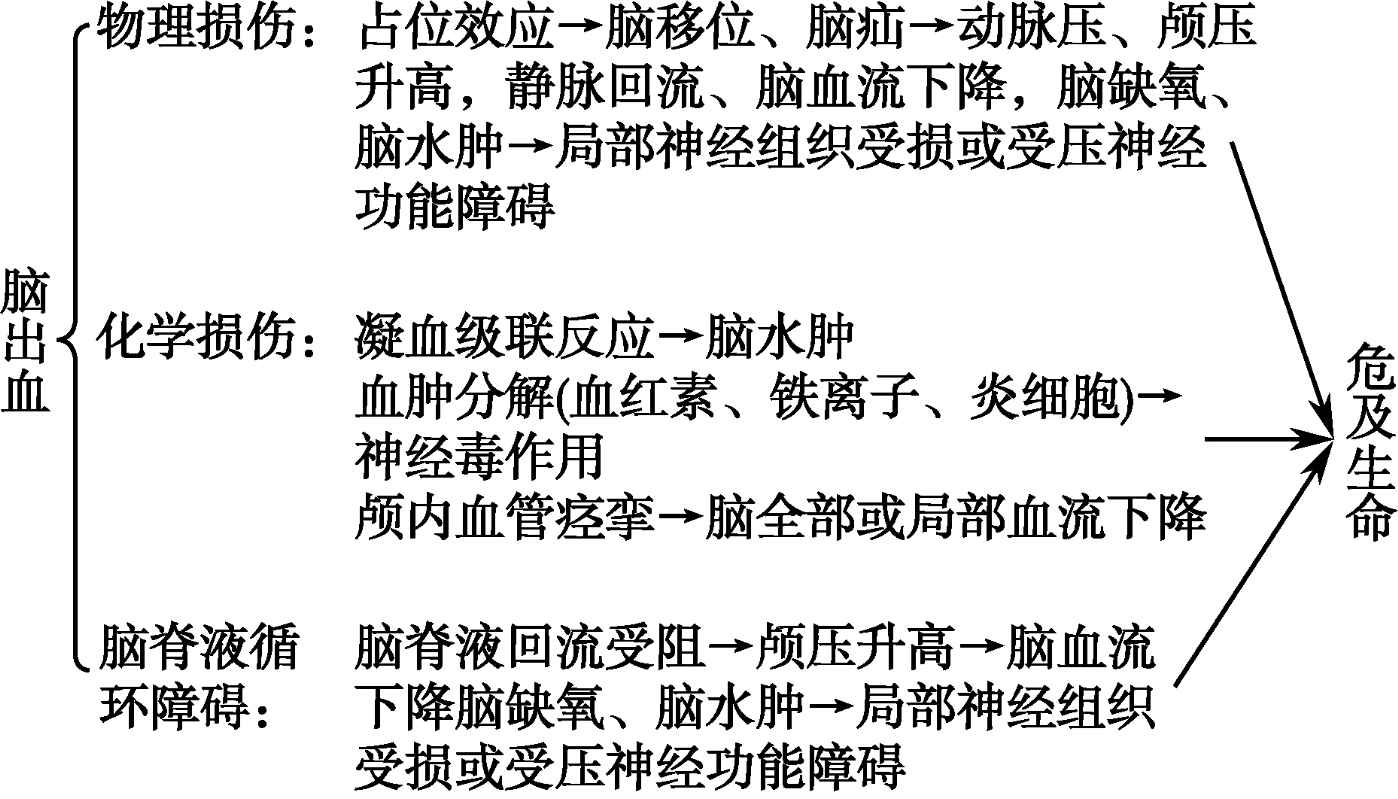
\includegraphics[width=3.09375in,height=1.76042in]{./images/Image00376.jpg}
 \captionsetup{justification=centering}
 \caption{高血压脑出血的病理生理变化}
 \label{fig84-1}
  \end{figure} 

\subsection{诊断}

\subsubsection{临床表现特点}

脑出血多发生于50岁以上伴有高血压的患者,尤其是60~70岁更多见。但是,近年来50岁以下的患者有增加的趋势,性别差异不大,在一年四季中皆可发病,以寒冷或气温骤变时节发生较多;发病通常在情绪激动、精神紧张、剧烈活动、用力过度、咳嗽、排便等情况下,使血压升高而发病,但也可在安静无活动状态下发病;多发生于体型肥胖、脸面潮红、颈短肩宽的患者,部分病例可有家族遗传史。起病常较突然,出血前多数无前驱症状,出血后临床表现的轻重与出血的部位、出血量、出血速度及代偿能力有很大的关系,还与以下因素有关:①出血的原发动脉;②血肿扩展的方向;③脑实质破坏的程度;④有否破入脑室。持续性出血致血肿扩大是病情加重的原因之一,血肿扩大易发生在基底节和丘脑患者,血肿的形态中不规则形发生率高于圆形或规则形。一般认为血肿体积增大超过首次CT血肿体积的50\%以上,或两次血肿体积相差20ml以上者为血肿扩大。表现为患者突然或逐渐意识障碍加深和血压持续升高。

\hypertarget{text00243.htmlux5cux23CHP8-1-3-2-1-1}{}
(一) 前驱期

一般病前无预感
,少数患者在出血前数小时或数天可有头痛、头晕、短暂意识模糊、嗜睡、精神症状、一过性肢体运动不便、感觉异常或说话不清等脑部症状,也可出现视网膜出血或鼻出血等其他症状。这些症状主要与高血压有关,并非脑出血特有的前驱症状。

\hypertarget{text00243.htmlux5cux23CHP8-1-3-2-1-2}{}
(二) 发病期

大多数患者起病急骤,常在数分钟或数小时内病情发展到高峰,也可在数分钟内即陷入昏迷,仅少部分患者发展比较缓慢,经数天才发展至高峰,类似缺血性脑梗死。其病程中一般有下述不同表现:①头痛:常为首发症状,表现为突发剧烈头痛,先位于患侧颞部,随后遍及全头或后枕部,乃血液刺激颅内疼痛敏感结构及颅内压升高所致。值得注意的是,失语患者仅能以手抚摸头部表示头痛;少量幕上脑出血和部分高龄患者仅有轻度头痛或不出现头痛。②头晕:可伴发于头痛,亦可为主要表现,多在后颅凹幕下出血时发生。③恶心呕吐:是早期症状之一,呕吐多因颅内压增高或脑干受损所致。头痛剧烈时表现更明显,但在幕下血肿时,头痛虽不剧烈,呕吐仍可非常频繁;如呕吐咖啡色物,则提示下丘脑受损。④意识障碍:极少量出血者可无明显意识障碍,轻者意识混浊、嗜睡,重者昏迷、去脑强直、高热。也有患者在出血几天后出现意识障碍,这可能与脑水肿及再出血有关。⑤血压增高:绝大多数的病例在170~250/100~150mmHg之间,这是由于原有高血压或由于颅内压增高、脑干缺血而导致血压代偿性增高所致。⑥瞳孔改变:一般大脑半球出血量不大时,瞳孔大小正常,光反应良好,有时病侧瞳孔较对侧小。如出现脑疝,动眼神经受压,出现同侧瞳孔散大,光反应迟钝或消失,边缘不齐。如病情继续加重,对侧瞳孔也散大。如脑干脑桥出血或脑室出血进入蛛网膜下腔,瞳孔常呈针尖样缩小。⑦其他:眼底检查可见动脉硬化、视网膜出血及视乳头水肿;出血进入蛛网膜下腔可出现脑膜刺激征;血肿占位与破坏脑组织可导致偏瘫、失语及眼位的改变等。总之,较典型的脑内出血首先表现为头痛、恶心、呕吐,经过数分至数小时后,出现意识障碍及局灶神经障碍体征,脉搏缓慢有力、面色潮红、大汗淋漓、大小便失禁、血压升高,甚至出现抽搐、昏迷程度加深、呈现鼾性呼吸,重者呈潮式呼吸,进而呼吸不规则或间停等,若出现脑疝则病情进一步恶化,出现脉快、体温高、血压下降、呕血等危险症状。

由于出血部位及范围不同可产生一些特殊定位性临床症状:

\paragraph{壳核 -内囊出血(图\ref{fig84-2})}

\begin{figure}[!htbp]
 \centering
 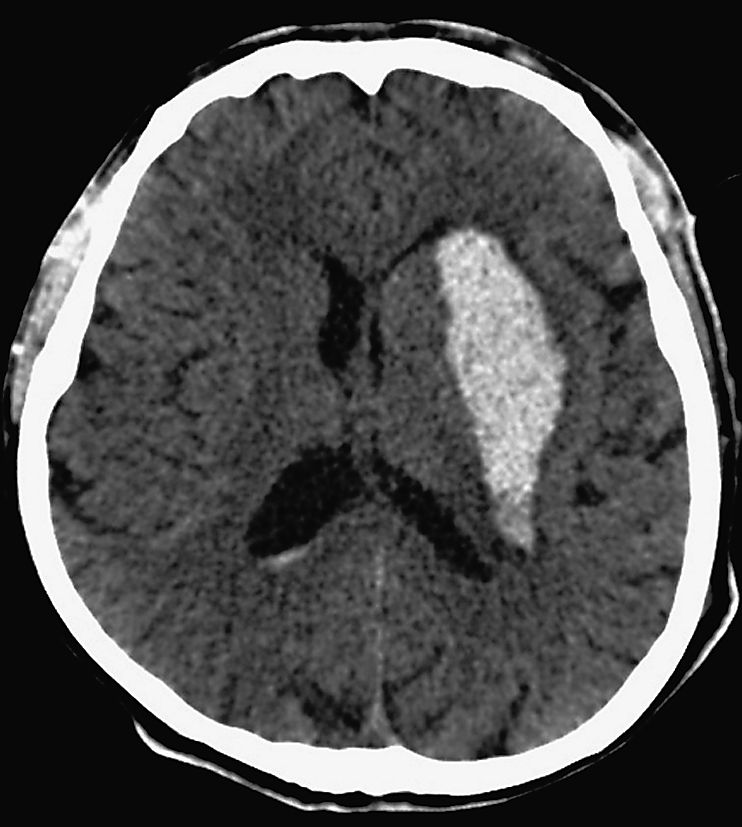
\includegraphics[width=2.46875in,height=2.75in]{./images/Image00377.jpg}
 \captionsetup{justification=centering}
 \caption{壳核出血}
 \label{fig84-2}
  \end{figure} 

临床最常见,约占脑出血的60\%。脑出血好发在壳核与豆纹动脉的外侧支易于破裂有关。因该支动脉最易破裂,又称之为出血动脉。豆纹动脉外侧支共3~6条,自大脑中动脉发出,与大脑中动脉几呈150°角发出,而大脑中动脉又是颈内动脉的直接延续,相距很近,故其管腔内压与颈内动脉的管腔内压相近,血流量也大,豆纹动脉分支处环状狭窄,在血压高时,该处承受压力较大,动脉硬化性改变亦较它处显著,故血压高时易于破裂。一般将壳核-内囊出血分为壳核外侧型(即外囊出血)和壳核内侧型(即内囊出血),壳核-内囊出血除具有脑出血的一般症状外,病灶对侧常出现偏瘫、偏身感觉障碍与偏盲等“三偏综合征”。临床上由于出血所累及的范围不同,“三偏”可不完全,最常见的是偏瘫、偏身感觉障碍。外侧型多无意识障碍,轻度偏瘫,预后较好;内侧型以血肿的量和发展的方向,临床上可出现不同程度的病变对侧中枢性面瘫及肢体瘫痪,感觉障碍和同向性偏盲。双眼向病灶侧凝视,呈“凝视病灶”。优势半球病变可有失语。如血肿破入脑室,或影响脑脊液循环时昏迷加深、偏瘫完全、头痛、呕吐、瞳孔不等大、中枢性高热、消化道出血,死亡率高。

\paragraph{丘脑出血(图\ref{fig84-3})}

约占脑出血的20\%~25\%,多见于50岁以上,有高血压动脉硬化的病史。常为丘脑膝状体动脉或丘脑穿动脉破裂出血,前者常为丘脑外侧核出血,后者常为丘脑内侧核出血。丘脑出血的血肿部位很深,位于基底节和内囊的内侧,故又称为内侧型出血。丘脑出血几乎都有眼球运动障碍,如下视麻痹、瞳孔缩小等。小量出血局限丘脑或对内囊有一定的影响,在临床上以偏身感觉障碍为主,无意识障碍或有轻微意识障碍,可有轻偏瘫、不自主运动,预后良好。丘脑出血破入脑室多数经第三脑室侧壁或侧脑室的下壁进入脑室。临床表现有明显的意识障碍,甚至昏迷,对侧肢体完全性瘫痪,颈项强直等脑膜刺激征表现。丘脑内侧或下部出血,出现双眼内收下视鼻尖,上视障碍,这是丘脑出血的典型体征。如出血少量破入脑室者,临床症状可出现缓解,大量出血破入脑室或造成梗阻性脑室扩张者使病情加重,如抢救不及时,可引起中枢性高热、四肢强直性抽搐以及脑-内脏综合征,甚至脑疝的表现。优势半球病变可出现各种类型的语言障碍,可为运动性或感觉性失语。有的病例缄默不语,语言错乱,句法错误,重复语言或阅读错误等;偏身感觉障碍常较运动障碍为重,深感觉障碍比浅感觉障碍为重。出血后很快出现昏迷者提示出血严重,所以丘脑出血的临床表现常呈多样性。

\begin{figure}[!htbp]
 \centering
 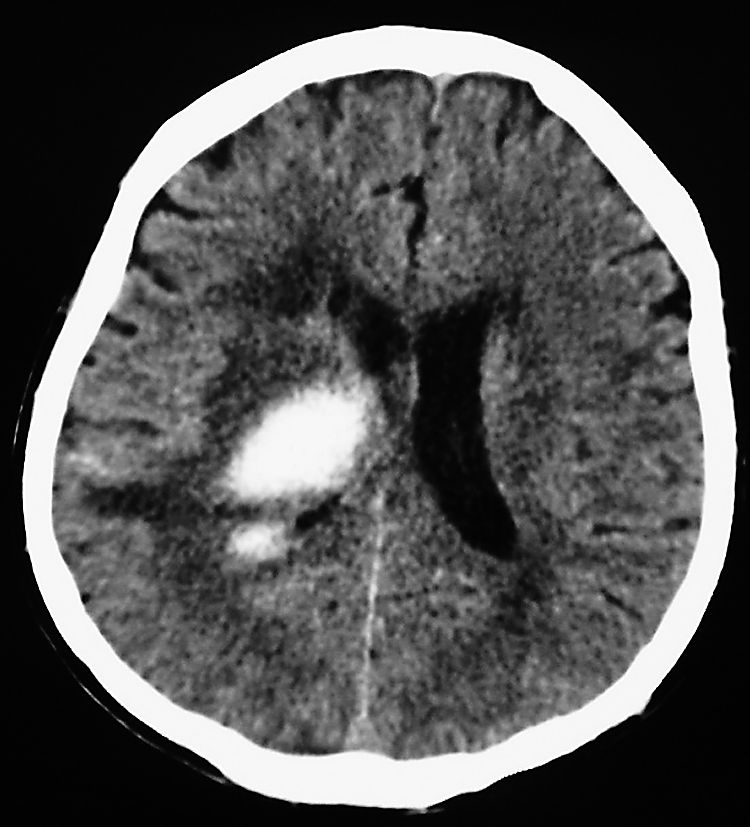
\includegraphics[width=2.5in,height=2.75in]{./images/Image00378.jpg}
 \captionsetup{justification=centering}
 \caption{丘脑出血}
 \label{fig84-3}
  \end{figure} 

\paragraph{脑叶出血(图\ref{fig84-4})}

又称皮质下白质出血,约占脑出血的13\%~18\%,是指发生在额叶、颞叶、顶叶、枕叶等部位的出血,是皮层下动脉破裂所致,原因多为脑动脉淀粉样变性所致。绝大多数呈急性起病,多先有头痛、呕吐或抽搐,甚至尿失禁等临床表现;意识障碍少而轻;偏瘫较基底节出血少见,而且较轻,有昏迷者多为大量出血压迫脑干所致。受累脑叶可出现相应的神经缺损症状,颞顶叶出血可有同向偏盲、偏瘫、失语;额叶出血可有智力障碍、尿失禁等;枕叶出血则可有一过性黑矇等。

\begin{figure}[!htbp]
 \centering
 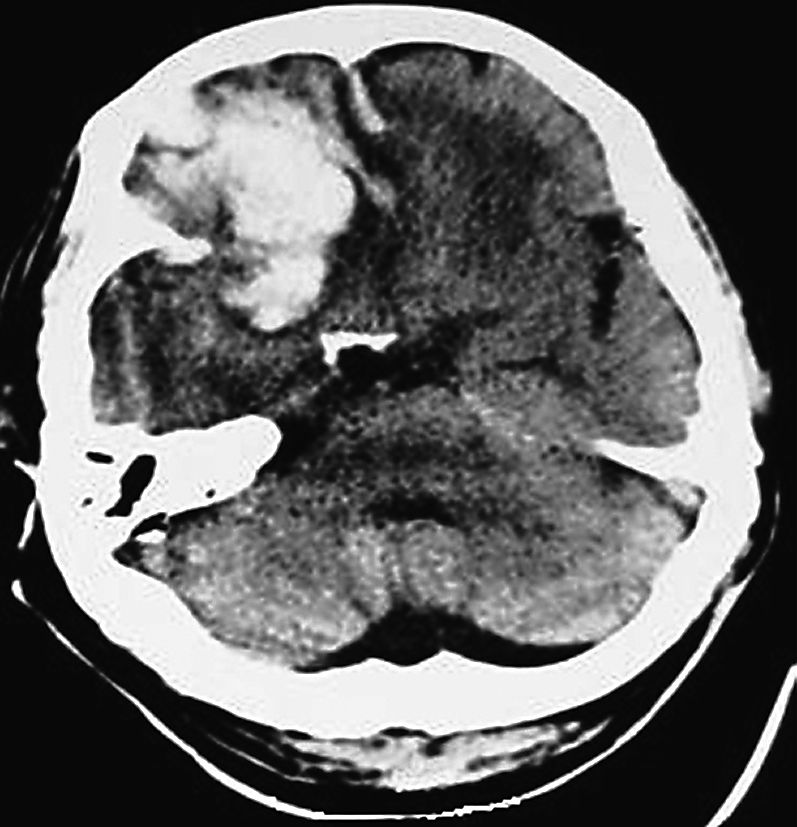
\includegraphics[width=2.65625in,height=2.75in]{./images/Image00379.jpg}
 \captionsetup{justification=centering}
 \caption{脑叶出血}
 \label{fig84-4}
  \end{figure} 

\paragraph{小脑出血(图\ref{fig84-5})}

\begin{figure}[!htbp]
 \centering
 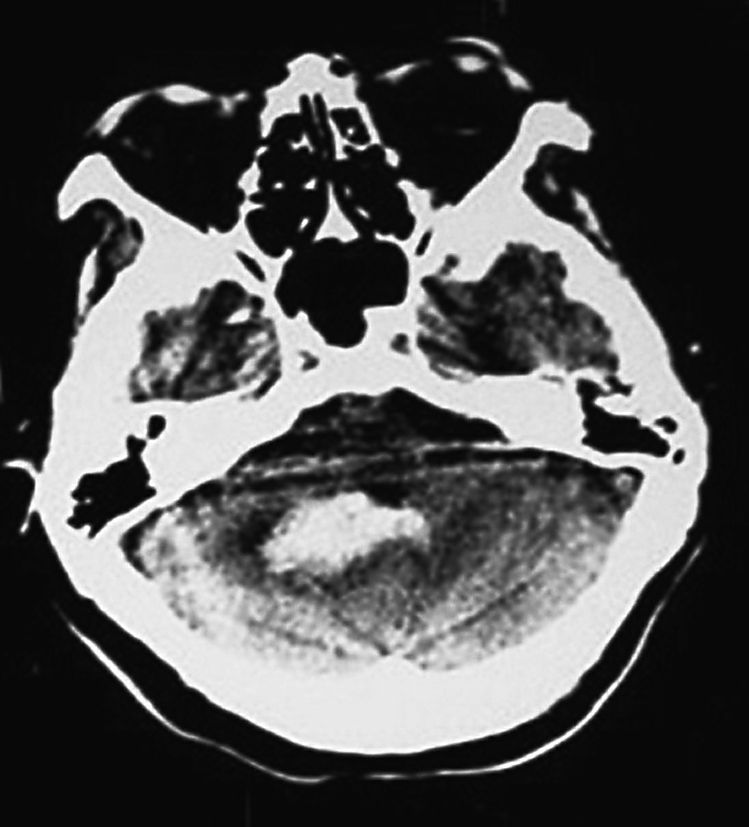
\includegraphics[width=2.48958in,height=2.75in]{./images/Image00380.jpg}
 \captionsetup{justification=centering}
 \caption{小脑出血}
 \label{fig84-5}
  \end{figure} 

约占10\%,好发于一侧小脑半球齿状核部位,多见于小脑上动脉的分支破裂出血,临床上可分为小脑半球和蚓部出血。多表现为突然发作的枕部头痛、眩晕、呕吐、肢体或躯干共济失调及眼球震颤等,当出血量较大锥体束受压迫时,可出现肢体瘫痪,当血肿影响到脑干和脑脊液循环通路,出现脑干受压和急性梗阻性脑积水,表现为双瞳孔缩小、眼球分离、双侧锥体束征阳性及脑神经损害症状,部分患者出现强迫头位、颈强直等。小而局限的出血,多无意识障碍,只有CT检查方可确诊;重者短时间内迅速昏迷,发生小脑扁桃体疝等致突然死亡。也有部分患者呈现出进行性加重,逐渐出现昏迷和脑干受压的体征,如不能得到及时正确的治疗,多在48小时内死亡。

\paragraph{原发性脑干出血(图\ref{fig84-6})}

90\%以上的高血压所致的原发性脑干出血发生在脑桥,少数发生在中脑。脑干出血一直被认为是发病急骤,死亡率很高,预后很差的疾病。中脑出血:侵犯一侧大脑脚则同侧眼球神经麻痹,伴对侧肢体瘫痪(Weber综合征)。脑桥出血:症状取决于出血灶的部位和大小,常突然剧烈头痛、恶心、呕吐、头晕或眩晕,一侧或双侧肢体乏力,偏身或半侧面部麻木;大量出血常迅速出现深昏迷,瞳孔明显缩小呈针尖样,但对光反射存在;四肢瘫痪,双侧锥体束体征阳性,高热,呼吸不规则,血压不稳;头眼和前庭反射消失,部分患者并发消化道出血,病情进行性恶化,多在短时间内死亡。出血量小者,可有核间型眼球运动麻痹、外展麻痹、面神经麻痹、偏瘫、交叉性麻痹或四肢瘫、双下肢瘫等。延髓出血:一经出现即迅速死亡。

\begin{figure}[!htbp]
 \centering
 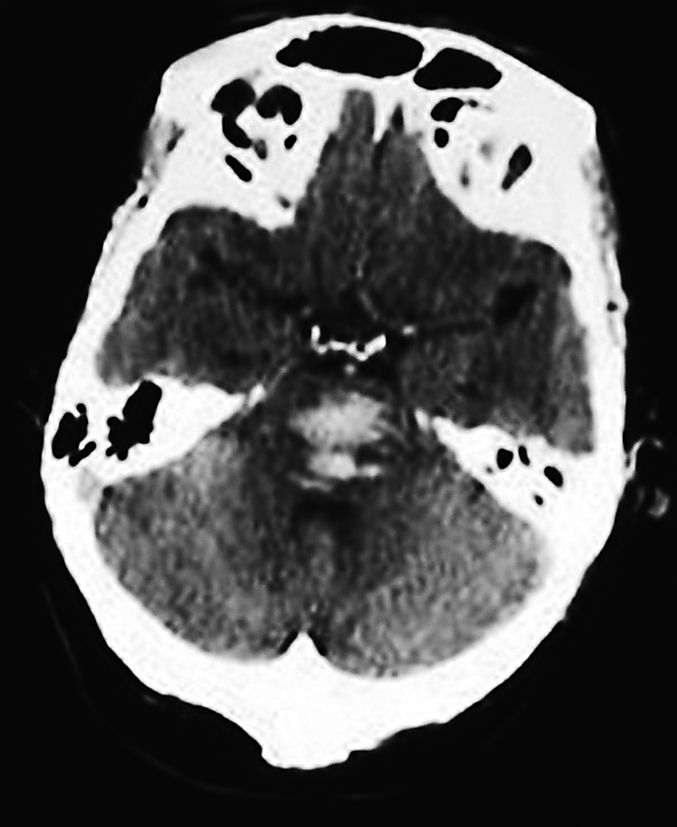
\includegraphics[width=2.25in,height=2.75in]{./images/Image00381.jpg}
 \captionsetup{justification=centering}
 \caption{原发性脑干出血}
 \label{fig84-6}
  \end{figure} 

\paragraph{脑室出血(图\ref{fig84-7})}

分为原发性和继发性两种。原发性脑室出血是指出血来源于脑室脉络丛,脑室内和脑室壁的血管,以及室管膜下1.5cm以内的脑室旁区的出血。临床表现主要是血液成分刺激引起的脑膜刺激征和脑脊液循环梗阻引起的颅内压增高症状;临床上见到的脑室出血绝大多数是继发性脑室出血。继发性脑室出血除了具有上述原发性脑室出血的临床特征外,还同时伴有原发性出血灶导致的神经功能障碍症状。因此,轻者仅有头痛、恶心、呕吐、颈强直等脑膜刺激征,无局灶性神经损害症状;重者表现为意识障碍、抽搐、肢体瘫痪、肌张力增高、瞳孔缩小或大小不定,双侧病理反射阳性等。血凝块堵塞室间孔、中脑导水管及第四脑室侧孔者,可因急性脑积水而致颅内压急剧增高,迅速发生脑疝而死亡。

\begin{figure}[!htbp]
 \centering
 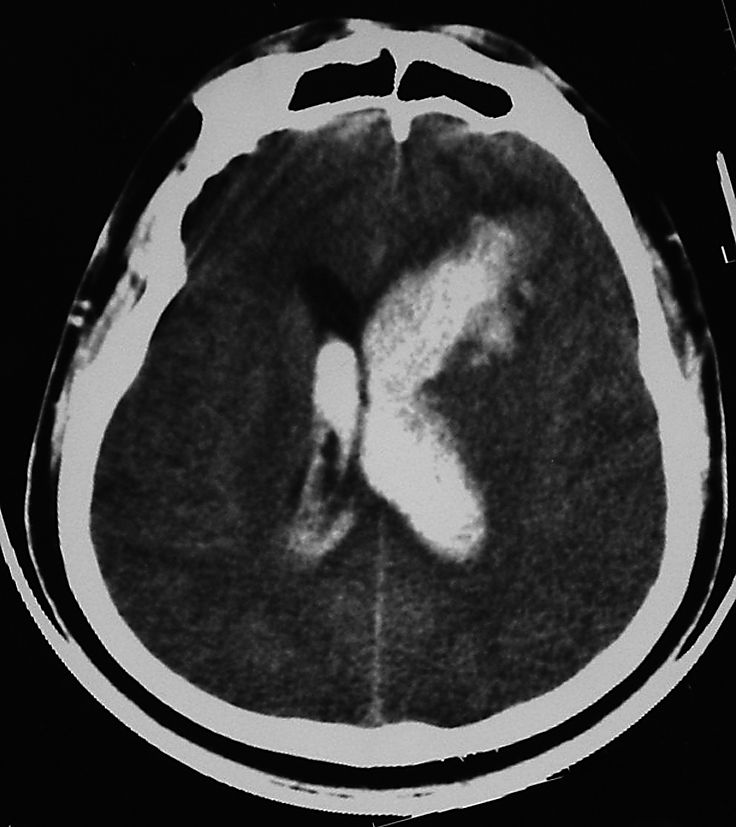
\includegraphics[width=2.44792in,height=2.75in]{./images/Image00382.jpg}
 \captionsetup{justification=centering}
 \caption{脑室出血}
 \label{fig84-7}
  \end{figure} 

\subsubsection{辅助检查}

\paragraph{颅脑 CT扫描}

CT扫描的问世,为脑出血的诊断和鉴别诊断提供了一种准确可靠的工具,在高清晰度的CT图像上,脑出血的诊断几乎可达100\%。它不仅为脑出血的定性、定位与定量诊断提供了可靠依据,而且可以直观反映血肿的形态、扩展方向、破入脑室的程度及其所致的脑水肿、脑结构移位情况等。因此,CT检查既是有效的诊断方法,也是制订治疗方案、观察疗效、判断预后的重要依据。对疑有脑出血的患者,应首选CT扫描检查,并应尽早进行,必要时还应多次检查,观察血肿的动态变化。脑出血依据病期不同,CT表现亦异。

\hypertarget{text00243.htmlux5cux23CHP8-1-3-2-2-1-1}{}
(1) 急性期(血肿形成期):

发病后1周内:血液溢出血管外形成血肿,其内含有大量血红蛋白、血浆白蛋白,球蛋白,因这些蛋白对X线的吸收系数高于脑质,故CT呈现高密度阴影,CT值达40~90H,最初高密度灶呈非均匀一致性,中心密度更高,新鲜出血灶边缘不清。①形态及大小:基底节区血肿多为“肾”型,内侧凹陷,外侧膨隆,因外侧裂阻力较小,故向外凸,其他部位血肿多呈尖圆形或不规则形,血肿出血量通常以多田民方程式计算,即π/6
×长(cm)×宽(cm)×高(cm)=出血量(ml);②周围水肿带:一般于出血后第二天开始出现水肿带,呈均匀低密度区,环绕于血肿周围,起初范围较小,第一周范围较大,出现率达95\%以上,以后逐渐减轻,持续一个月左右消退。③占位表现:由于血肿及周围水肿,使邻近脑室受压移位,甚至完全闭塞,中线结构亦向对侧移位,这种占位效应的出现及严重程度与脑出血量及速度有关,可见于75\%以上的病例;④破入脑室:大约25\%的病例血肿破入脑室,使脑室密度增高,完全充满血液者形成高密度的脑室铸形;未完全充满脑室者血液多沉积于脑室后角,以同侧最明显,可见一高密度影。

\hypertarget{text00243.htmlux5cux23CHP8-1-3-2-2-1-2}{}
(2) 血肿吸收期:

此期大约从2周~2个月,自第2周开始血肿周边的血红蛋白逐渐破坏,纤维蛋白溶解,使周围低密度带逐渐加宽,血肿高密度影呈向心性缩小,边缘模糊,一般于第四周变为等密或低密度区。

增强检查:在2周~2个月期间,90\%的血肿周围可出现环状强化,此环可直接反映原血肿的大小和形态,随着增强检查的时间推移,环内可出现高密度,等密度或低密度,强化环较薄,大约6mm厚,CT值为32~55H,一般认为强化环的出现是由于血肿周围含有增生的肉芽组织,血管自身调节力丧失,血液过度灌注及血脑屏障破坏等因素所致。

\hypertarget{text00243.htmlux5cux23CHP8-1-3-2-2-1-3}{}
(3) 囊腔形成期:

发病2个月后血肿一般即完全吸收,周围水肿消失,不再有占位表现呈低密度囊腔,其边缘清楚,不再出现强化环,CT值近脑脊液,较小的出血灶则形成纤维瘢痕,邻近的脑室或脑沟代偿性扩大。

\paragraph{颅脑 MRI扫描}

脑出血后,MRI主要显示的是血肿和血肿周围组织水肿演变过程中所形成的影像,它实际上反映了出血区红细胞的溶解和血红蛋白分子的化学变化过程。在MRI图像上,血肿信号的强弱受红细胞铁离子的影响。出血后,红细胞内所含血红蛋白历经氧合血红蛋白、脱氧血红蛋白、正铁血红蛋白、含铁血红素的变化过程。血红蛋白变化过程中不同阶段的物质所含铁离子的数量和不成对电子的数量都不相同,它们在构成这些物质的分子中的分布不相同,因而所产生的顺磁性效应也不相同。

从MRI的影像上分析:脑内血肿可分为5期:即超急性期、急性期、亚急性期、慢性期、残腔期。

\hypertarget{text00243.htmlux5cux23CHP8-1-3-2-2-2-1}{}
(1) 超急性期:

指脑内出血24小时以内,此时出血灶的血浆尚未吸收,血肿主要由完整红细胞内的含氧血红蛋白组成,因此,在T\textsubscript{1}
加权像(TR <
600ms)上呈低信号、略高信号或等信号,在质子密度加权像上呈高信号或等信号,在T\textsubscript{2}
加权像(TR > 1500ms)上呈高信号。

\hypertarget{text00243.htmlux5cux23CHP8-1-3-2-2-2-2}{}
(2) 急性期血肿:

出血在1周内,出血几小时内病灶区血浆成分即开始吸收,血细胞比容逐渐升高,同时含氧血红蛋白(HbO\textsubscript{2}
)因缺氧而变成脱氧血红蛋白(DHb),伴周围脑组织水肿。因此,急性期血肿本身与灰质相比,在T\textsubscript{1}
加权像(TR < 600ms)上呈等信号或略低信号,在T\textsubscript{2}
加权像(TR > 1500ms,高场强)上呈低信号。其中,以T\textsubscript{2}
加权像最有意义,即T\textsubscript{2}
加权像上的低信号区相当于CT上的高密度影。当红细胞内的DHb逐渐演变成正铁血红蛋白(MHB)后,在T\textsubscript{1}
加权像上呈高信号,在T\textsubscript{2}
加权像上仍呈低信号,而且比DHb更低。总之,急性期血肿的典型表现是T\textsubscript{2}
加权像上呈短T\textsubscript{2}
低信号。急性血肿周围的脑水肿在发病后24~48小时即可在MRI上显示。与灰质相比,脑水肿在T\textsubscript{1}
加权像上呈低信号,在T\textsubscript{2}
加权像上呈高信号,脑水肿在T\textsubscript{2}
加权像上显示得最清楚,在发病数周后才会消失。

\hypertarget{text00243.htmlux5cux23CHP8-1-3-2-2-2-3}{}
(3) 亚急性血肿:

出血后1周~1个月。在出血后1周左右,血肿周边部的脱氧血红蛋白(DHb)全已变成正铁血红蛋白(MHb),此时红细胞已溶解,也就是说,出血后第1周左右血肿周边部主要由游离而稀释的MHb组成,由于DHb先从血肿周边部转化为MHb,因此,亚急性血肿早期在T\textsubscript{1}
加权像上血肿周边部呈明显环状高信号,血肿中心呈低信号,此乃亚急性血肿早期的MRI特征;在质子密度加权像上血肿周边部呈球状略高信号,血肿中心呈等或略低信号;在T\textsubscript{2}
加权像上血肿周边部呈明显环状高信号,血肿中心呈等或低信号。周围脑水肿依然存在。在以后的2~3周内,DHb进行性地变成MHb,从血肿周边向中心蔓延。因此,在T\textsubscript{1}
加权像上高信号环从周边部向中心扩展,直至充满整个血肿。在质子密度加权像及T\textsubscript{2}
加权像上也逐渐变成高信号。在上述演变过程中,T\textsubscript{2}
加权像比T\textsubscript{1} 加权像缓慢,此时,周围脑水肿依然存在。

\hypertarget{text00243.htmlux5cux23CHP8-1-3-2-2-2-4}{}
(4) 慢性期血肿:

出血1个月之后,此时红细胞均已溶解,慢性血肿由稀释的游离MHb组成,后者在所有的加权像中均为高信号,反应性巨噬细胞积聚血肿周边,消化血红蛋白产物,在细胞质内以不溶性含铁血黄素颗粒的形式沉淀下来,形成含铁血黄素环。该环在T\textsubscript{1}
加权像上呈等或略低信号,在质子密度加权像上呈等或略低信号,在T\textsubscript{2}
加权像上呈明显低信号。此时血肿周围脑水肿已消散,总之,慢性血肿的MR特征为:高信号血肿,外加一个低信号含铁血黄素环。

\hypertarget{text00243.htmlux5cux23CHP8-1-3-2-2-2-5}{}
(5) 血肿残腔期:

见于出血2个月后至数年。从2个月后血肿出现囊变液化,当慢性血肿内的所有液体被吸收后,仅留下一个含铁血黄素衬边的残腔,即脑实质内塌陷的血肿残腔。在T\textsubscript{1}
加权像上呈低信号,在T\textsubscript{2}
加权像上呈明显低信号。总之,陈旧性血肿的MRI特征为低信号残腔。

尽管目前CT仍是急性脑内出血的首选检查方法,但MRI诊断亚急性与慢性血肿比CT敏感,尤其对陈旧血肿,MRI可清晰显示含铁血黄素衬边的低信号残腔,容易与陈旧性脑梗死鉴别。

\paragraph{脑血管造影(DSA)}

脑出血患者一般不需要进行DSA检查,除非临床上怀疑有血管畸形、血管炎或Moyamoya病又需外科手术或血管介入治疗时才考虑进行。DSA可清楚显示异常血管和造影剂外漏的破裂血管及部位。

\paragraph{腰椎穿刺}

在CT广泛应用后,已无需采用腰椎穿刺诊断脑出血,以免诱发脑疝形成,如需排除颅内感染和蛛网膜下腔出血,可谨慎进行。

\subsubsection{诊断注意事项}

中老年患者在活动中或情绪激动时突然发病,迅速出现局灶性神经功能缺损症状以及头痛、呕吐等颅高压症状应考虑ICH的可能,结合头颅CT/MRI检查,可以迅速明确诊断。鉴别诊断方面:①首先应与急性脑梗死、蛛网膜下腔出血等鉴别(参见表\ref{tab84-2});②颅内肿瘤出血:颅内肿瘤,特别是原发性肿瘤,多因生长速度快而致肿瘤中心部位的缺血、坏死,易与脑出血相混。但肿瘤患者,病程较长,多在原有症状的基础上突然加重,也可为首发症状。增强的头颅CT和MRI对肿瘤出血具有诊断价值。③对发病突然、迅速昏迷且局灶体征不明显者,应注意与引起昏迷的全身性疾病如中毒(酒精中毒、镇静催眠药物中毒等)及代谢性疾病(低血糖、肝性脑病、肺性脑病等)鉴别;④对有头部外伤史者应与外伤性颅内血肿相鉴别。

脑出血患者的病情分级见表\ref{tab84-7}。

\begin{table}[htbp]
\centering
\caption{脑出血病情分级}
\label{tab84-7}
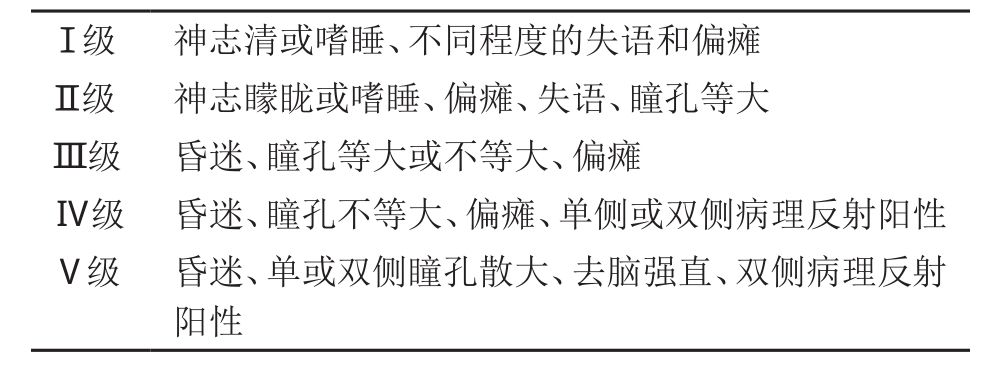
\includegraphics[width=3.27083in,height=1.22917in]{./images/Image00383.jpg}
\end{table}

\subsection{治疗}

脑出血是急性脑血管疾病中常见病之一,其病程可分为急性期、恢复期及后遗症期。急性期指发病后的3周内,此期脑组织受到破坏、水肿严重、脑功能紊乱,机体处于应激状态,死亡率高。恢复期和后遗症期主要是功能的恢复过程。因此,急性期的治疗极其重要。急性期的治疗主要包括现场急救处理、内科治疗和手术治疗。

\subsubsection{现场急救处理}

预诊护士必须及时接待患者,快速反应,准确分诊,尽快将患者送到诊室。对昏迷患者须保持呼吸道通畅,可将头歪向一侧,或侧卧位,头部抬高20°,给予吸氧并及时清除口腔和呼吸道分泌物,对呼衰患者必要时行气管切开给予人工通气。接诊医师简明扼要询问病史,做较全面体检,对血压过高、脑疝危象、抽搐者给予及时处理;各种检查妥善安排,尽量减少不必要的搬动。对危重患者及时开通静脉。对暂时无法收住院的危重患者,留置抢救室或诊室内抢救治疗,并做好交接班。对濒死无法抢救的患者,在向家属交代病情的同时,给予人道主义处理。

\subsubsection{内科治疗}

急性期内科治疗原则是制止继续出血和防止再出血,减轻和控制脑水肿,预防和治疗各种并发症,维持生命体征。治疗的主要目的是挽救患者生命,降低残疾率,防止复发。

\paragraph{一般治疗}

①一般应卧床休息2~4周,保持安静,避免情绪激动和血压升高。严密观测生命体征,注意瞳孔和意识变化。②保持呼吸道通畅,给氧,防止并发症:对意识不清的患者应及时清除口腔和鼻腔的分泌物或呕吐物,头偏向一侧,或侧卧位。若PaO\textsubscript{2}
< 60mmHg或PaCO\textsubscript{2} >50mmHg应吸氧,使SaO\textsubscript{2}
维持在90\%以上,PaCO\textsubscript{2}
保持在25~35mmHg之间,必要时气管插管或行气管切开术。③保持水、电解质平衡及营养支持:有意识障碍、消化道出血者宜禁食24~48小时,并适当静脉输液,每日入液量可按尿量+
500ml计算,如有高热、多汗、呕吐或腹泻者,可适当增加入液量。48小时后,如果意识好转,且吞咽无障碍者可试进流质,少量多餐,否则应下胃管鼻饲维持营养。注意防止低钠血症,以免加重脑水肿。④控制血糖:维持血糖水平在6~9mmol/L之间。⑤明显头痛、过度烦躁不安者,可适当应用镇静止痛剂;便秘者可用缓泻剂。⑥保持功能体位,防止肢体畸形:卧位上肢应处于轻度外展,肘轻屈,肩胛处、前臂和手用枕头支托,掌心向上,使前臂保持旋后位,防止肩胛骨后撤。下肢骨盆、臀部用枕头支托,防止下肢外旋和骨盆后坠,下肢肌张力高的患者,应采取侧卧位;患侧卧位时,患侧肩部向前伸,肘伸展,掌心向上,如手指屈曲,肌张力高,大拇指与其他四指用布卷或纸卷隔开。下肢稍屈曲,脚掌与下腿尽量保持垂直;健侧卧位时,患侧上肢下垫一枕头,上肢伸直,掌心向下,手腕略微抬起。

\paragraph{控制血压}

脑出血后一般血压都高,这是因为颅内压增高是为了保证脑组织供血的代偿性反应,当颅内压下降,血压也下降。因此,一般不需要给降压药物。但是,如收缩压大于200mmHg时,血压越高,脑血流量越下降,此时应该持续静脉应用降压药物快速降压。早期降低过高的血压,是防止进一步出血的关键。脑出血急性期血压高,可首先脱水降颅压,脱水后血压仍过高,应给予降血压治疗。因此,在脑出血急性期,当血压≥200/110mmHg时,应采取降压治疗,使血压维持在略高于发病前水平;当血压<
180/105mmHg时,可暂不使用降压药物。SBP在180~200mmHg或DBP在100~110mmHg之间时,需密切监测血压;即使应用降压药物治疗,也需避免应用强力降压药物,防止因血压下降过快引起脑低灌注。如果不了解病前的血压,可把血压维持在160/100mmHg左右,这样的血压可保证脑的灌流。在使用降压药物时,应使血压较缓慢地下降,避免血压下降过快、过低。降压目标:MAP维持在130mmHg左右。药物选择有乌拉地尔、非诺多泮、尼卡地平、拉贝洛尔等。

对低血压的处理,要首先分析原因,区别情况加以处理。引起低血压的原因如下:①脱水过量、补液不足;②大量呕吐失水或伴有应激性溃疡导致失血;③并发严重的感染;④心力衰竭、心律失常;⑤降压药、镇静剂及血管扩张药使用过量;⑥呼吸不畅并酸中毒;⑦脑疝晚期等。在针对病因处理的同时,可静滴多巴胺、间羟胺(阿拉明)等,将血压提升并维持在150/90mmHg左右为宜。

脑出血恢复期应积极控制血压,尽量将血压控制在正常范围内。

\paragraph{控制脑水肿 、降低颅内压}

脑出血后脑水肿约在48小时达高峰,维持3~5天后逐渐消退,可持续2~3周或更长。脑水肿可使颅内压(intracranial
pressure,ICP)增高,并致脑疝形成,是影响ICH死亡率及功能恢复的主要因素。积极控制脑水肿、降低ICP是ICH急性期治疗的重要环节。常用脱水剂有:①20\%甘露醇:通常125~250ml,每6~8小时1次,疗程7~10天。如有脑疝形成征象可快速加压静滴或静推。冠心病、心肌梗死、心力衰竭和肾功能不全者宜慎用。②甘油果糖注射液:每瓶250ml;500ml。每1ml中含甘油100mg、果糖50mg、氯化钠9mg。成人一次250~500ml静滴,每天1~2次,儿童用量为5~10ml/kg。每500ml静滴需2~3小时,连续用1~2周。其脱水、降ICP作用较甘露醇缓和,用于轻症患者、重症患者的病情好转期和肾功能不全患者。和甘露醇联合应用,既迅速降颅压,改善症状,又减轻肾脏负担,保护肾功能,还克服了甘露醇的颅内压反跳现象。③甘油:口服剂量为1~2g/(kg•d),用生理盐水配成50\%的甘油盐水,每次30~50ml口服,每日3次。副作用为恶心、呕吐、腹胀。10\%复方甘油注射液,成人每次500ml,以100~150ml/h速度静脉输入,每日1~2次。注射后2~4小时发挥作用,持续18小时。④高渗盐水:适用于并发低钠血症的颅内压增高患者。⑤人血白蛋白:对血容量不足、低蛋白血症的颅内高压、脑水肿患者尤为适用。因其增加心脏负荷,有心功能不全者须慎用。用法:10\%人血白蛋白50~100ml静滴,每日1次。⑥利尿剂:常用呋塞米每次20~40mg,每日2~4次肌注或静注;布美他尼(丁尿胺)每次0.5~1mg肌注或静注,必要时30分钟后重复使用一次。常与甘露醇交替使用可增强脱水效果。不建议用激素治疗减轻脑水肿。脱水治疗时要注意水、电解质平衡及监测肾功能。

\paragraph{止血治疗}

止血药物如6-氨基己酸、氨甲苯酸、注射用血凝酶(立止血)等对高血压性脑出血的作用不大。如有凝血功能障碍,可针对性给予止血药物治疗,例如肝素治疗并发的脑出血可用鱼精蛋白中和,华法林治疗并发的脑出血用维生素K\textsubscript{1}
拮抗。

\paragraph{防治并发症}

①感染:发病早期病情较轻又无感染证据者,一般不建议常规使用抗生素;合并意识障碍的老年患者易并发肺部感染,或因导尿等易合并尿路感染,可给予预防性抗生素治疗;若已经出现系统感染,则根据经验或药敏结果选用抗生素。②应激性溃疡:对重症或高龄患者应预防应用H\textsubscript{2}
RB/PPI。一旦出血按上消化道出血的治疗常规进行。③抗利尿激素分泌异常综合征:即稀释性低钠血症,可发生于约10\%
ICH患者。因经尿排钠增多,血钠降低,加重脑水肿。应限制水摄入量在800~1000ml/d,补钠9~12g/d。低钠血症宜缓慢纠正,否则可致脑桥中央髓鞘溶解症。④脑耗盐综合征:系因心钠素分泌过高所致的低钠血症,治疗时应输液补钠。⑤痫性发作:有癫痫频繁发作者,可静脉注射地西泮10~20mg,或苯妥英钠15~20mg/kg缓慢静注以控制发作。⑥中枢性高热:多采用物理降温,可试用溴隐亭治疗。⑦下肢深静脉血栓形成或肺栓塞:一旦发生,应给予普通肝素100mg/d静滴,或低分子肝素4000U皮下注射,每天2次。对高龄、衰弱的卧床患者可预防性治疗。

\paragraph{脑保护剂的应用与低温疗法}

脑出血后,出血灶周边的脑组织受压迫,导致血液循环障碍,继发脑水肿、脑缺血;如血液破入脑室或蛛网膜下腔还可引起脑血管痉挛;另外,颅内压增高,可引起全脑受损,因此有必要给予脑保护治疗。常用的药物有:尼莫地平、维生素E、维生素C。甘露醇也有清除自由基的作用,地塞米松有稳定细胞膜、清除自由基、保护脑细胞的作用。低温可以降低细胞的代谢率,抑制脑单胺和兴奋性氨基酸递质的合成和释放,对损伤的脑组织有确切的保护作用。但是要真正达到大脑深部的低温很难做到,目前常用的头枕冰袋、冰帽可起到一定的作用。冬眠疗法配合使用冰毯、冰帽可使全身的体温下降至35℃,起到脑保护的作用,但影响意识状态,不利于疾病病情的观察,可根据具体情况,权衡利弊,酌情使用。

\subsubsection{手术治疗}

脑出血除药物治疗外,某些病例可考虑手术治疗。一般来说,脑出血一旦确诊,应首先给予脱水、降压等措施,根据血肿的大小、部位、患者的一般状况及临床表现来适时决定是否进行手术治疗。关于手术治疗的指征,目前尚无统一的标准。总的来说,如以出血量来选择治疗原则:壳核出血大于30ml、丘脑出血大于15ml、小脑出血大于10ml,应行手术治疗;如以CT的出血范围来选择治疗原则:壳核出血发展到内囊后肢破入或不破入脑室、壳核出血发展到内囊的前后肢、丘脑出血量大于15ml,累及丘脑或丘脑下部,破入或不破入脑室,小脑出血伴神经功能恶化,脑干受压和(或)脑室梗阻致脑积水者均应考虑手术治疗;如按意识障碍的程度及临床症状的轻重来选择:患者处于昏睡、浅昏迷但无脑疝或脑疝早期、意识状态呈进行性加重,内科治疗无好转,应考虑手术。患者处于深昏迷、濒死状态、呼吸骤停、双侧瞳孔散大,有这种情况之一者应暂缓手术。高血压脑出血的手术方法应根据患者的出血量、出血部位、手术距离出血的时间、患者的年龄和全身情况以及手术者的经验来决定,个体化的原则同样适用于脑出血,对每个患者都要具体分析,全面考虑,做出决策。常用清除血肿的手术方法有以下几种:

\paragraph{神经内镜治疗技术}

是在颅骨上钻一个小孔,送入颅内镜,直达血肿部位。在电子监视设备的引导下,利用导管上的通道,一边在出血点直接给药止血,一边清理吸出残留的凝血块。具有手术时间短、创伤小等优点,避免了开颅手术对脑组织大量暴露、切开、牵拉等可能带来的后遗症,有助于患者的迅速康复。

\paragraph{定向软管血肿吸引术}

也称方体定向软管吸引术,是近年来国内新兴的一种微创救治新技术,可在病房床边或CT下可视操作完成。它是利用方体定向原理对脑出血部位准确定位后,定向锥颅建立进入颅内血肿靶点通道,并由此在出血部位置入一根或多根软的硅胶管吸引血肿,术后反复注入纤溶药物,将血凝块溶解,由置入的硅胶管流出。此种术式具有简便价廉、恢复快等优点,适合危重患者的早期救治,有助于患者早期康复。

\paragraph{开颅血肿清除术}

是传统术式,但对血肿很大或已出现脑疝的危重患者,开颅在直视下彻底清除血肿、止血,并行减压术仍是一种可行的手术方法,近年来显微外科技术的应用可使手术更为安全精细。

\subsection{预防}

脑出血常见原因是高血压合并动脉硬化。降低血压是预防脑动脉硬化的有效方法,可显著降低脑出血的发病率和死亡率。脑出血首次发作后,容易复发(每年2.4\%),尤其脑叶出血者。Bue等随访989例高血压脑出血患者,发现首次发作后,抗高血压治疗少于3个月者,复发的危险性明显高于长期抗高血压治疗者,提示长期有效的控制高血压有利于预防脑出血复发。美国卒中协会(ASA)2010年发表的诊疗指南认为:尽管最佳的血压控制目标还缺乏专门的研究证据,但是目前认可的合理的血压是小于140/90mmHg(或合并糖尿病和慢性肾损害者小于130/80mmHg),也即是目前高血压预防、诊断、评估和治疗联盟的建议。此外,戒烟、低盐、低脂、低胆固醇饮食在预防脑动脉硬化中的效果也不容忽视。

\hypertarget{text00243.htmlux5cux23CHP8-1-3-5}{}
参 考 文 献

1. Morgenstern LB,Hemphill JC 3\textsuperscript{rd} ,Anderson C,et
al. Guidelines for the management of spontaneous intracerebral
hemorrhage:a guideline for healthcare professionals from the American
Heart Association/ American Stroke Association.
Stroke,2010,41(9):2108-2129.

2.
孙树杰,等.方体定向吸引术治疗少量壳核出血疗效分析.中华实用诊断与治疗杂志,2010,24(9):907-908.

3. 孙树杰
,王畅.高血压脑出血的急诊综合治疗.中华急诊医学杂志,2009,18(12):1343-1344.

4.
孙树杰,等.长方体定位排空术救治高血压脑出血(附206例分析).中国微侵袭神经外科杂志,2009,14(5):213-215.

\protect\hypertarget{text00244.html}{}{}

\section{蛛网膜下腔出血}

蛛网膜下腔出血(subarachnoid
hemorrhage,SAH)是统指颅内血管破裂后,血液流入蛛网膜下腔的一种临床综合征。临床上通常分为自发性与外伤性两类。自发性又可分为原发性和继发性两类。凡出血系由于脑底部或脑表面的病变血管破裂,血液直接流入蛛网膜下腔者,称为原发性SAH,约占急性脑卒中的10\%左右;如系脑实质内出血,血液穿破脑组织而流入脑室及蛛网膜下腔者,则属继发性SAH,其病因以高血压脑动脉粥样硬化、血管炎、血液病等多见。本文只介绍原发性SAH。

\subsection{病因与发病机制}

原发性SAH病因以颅内动脉瘤为最常见(约占50\%~80\%),其中先天性粟粒样动脉瘤约占75\%,还可见高血压、动脉粥样硬化所致梭形动脉瘤及感染所致的真菌性动脉瘤等。血管畸形次之(约占SAH病因的10\%),其中动静脉血管畸形(arteriovenous
malformation,AVM)占血管畸形的80\%,多见于青年人,90\%以上位于幕上,常见于大脑中动脉分布区。其他病因有moyamoya病(占儿童SAH的20\%)、颅内肿瘤、血液系统疾病和抗凝治疗并发症等。约10\%患者病因不明。

动脉瘤好发于脑底动脉环的分叉处,最常见的部位为前交通动脉与大脑前动脉的接合处,后交通动脉与颈内动脉的接合处、大脑中动脉的分叉处、基底动脉的顶端、基底动脉及其主要分支的衔接处、椎动脉与小脑后下动脉的衔接处。85\%~90\%发生于颅底动脉环的前半部。由于该处动脉内弹力层和肌层的先天性缺陷,在血液涡流的冲击下渐向外突而形成动脉瘤。多呈囊状,一般只有绿豆到黄豆大小,多为单发,约20\%为多发。炎症动脉瘤是由动脉炎或颅内炎症引起的血管壁病变。AVM是一种先天发育异常的动静脉瘘,小的可仅数毫米;有的则随时间而长成一大堆迂曲、扩张的血管,动静脉分流量之大可使心输出量也增加。扩张、肥大的供血动脉从脑表面进入病损后,在皮质下分散为呈网状分布的薄壁血管,动脉血不经过正常的毛细血管网而直接输入引流静脉。动脉血的直接进入,使得这些管壁异常薄的血管增大、扩张,呈搏动性。AVM可发生于脑和脊髓的任何部位,但以大脑额顶区较常见,呈楔形,基底位皮质,顶朝向脑室,大的足以覆盖整个大脑半球。由于血管畸形,管壁变薄.最后终于破裂而致SAH或脑内出血,常二者兼有之。脑动脉粥样硬化时,脑动脉中纤维组织替代了肌层,内弹力层变性断裂和胆固醇沉积于内膜,加上血液的冲击,渐扩张而形成动脉瘤,多呈梭形,常见于脑底部的较大动脉的主干。其他如肿瘤或转移癌直接侵蚀血管,引起血管壁病变,最终导致破裂出血。

动脉瘤出血常限于蛛网膜下腔,不造成局灶性脑损害,神经系统检查很少发现局灶体征,除非大脑中动脉动脉瘤。而AVM破裂常见局灶性异常。

SAH能引起一系列病理生理改变:①血液流入蛛网膜下腔刺激痛觉敏感结构引起头痛,颅内容积增加使颅内压(ICP)增高可加剧头痛,导致玻璃体下视网膜出血,甚至发生脑疝。②颅底或脑室内血液凝固使CSF回流受阻,30\%~70\%的患者早期出现急性阻塞性脑积水,血红蛋白及含铁血黄素沉积于蛛网膜颗粒也可导致CSF回流受阻,出现交通性脑积水和脑室扩张。③蛛网膜下腔血细胞崩解释放各种炎症物质引起化学性脑膜炎,CSF增多使ICP增高。④血液及分解产物直接刺激引起下丘脑功能紊乱,如发热、血糖升高、急性心肌缺血和心律失常等。⑤血液释放的血管活性物质如5-HT、TXA\textsubscript{2}
和组织胺等可刺激血管和脑膜,引起血管痉挛,严重者致脑梗死。

\subsection{诊断}

\subsubsection{先兆和诱发因素}

SAH有1/3在发病前出现先兆征象或警告信号。常见者为全头痛、局限性头痛、嗜睡、眼球运动障碍、三叉神经分布区疼痛及项背部疼痛等。颈内动脉及大脑中动脉的动脉瘤在破裂之前可因血管痉挛、局部梗塞、小量出血及刺激压迫而引起对侧轻偏瘫、感觉异常及或失语;大脑前动脉瘤可引起同侧动眼神经麻痹及皮层性一过性黑矇等。近1/3患者有诱因如突然用力、兴奋、激动、屏气、大便、饮酒等。

\subsubsection{临床表现特点}

\paragraph{头痛}

80\%~90\%的患者最突出的症状是剧烈的局限性劈裂样头痛,多数患者是在意识恢复清醒后才诉头痛的。患者常描述为“一生中经历的最严重头痛”,新发生头痛最有临床意义。常伴颈项与背痛,面色苍白与全身冷汗。疼痛始于前半头部常示幕上出血,始于后枕部常示幕下出血,多与动脉瘤破损侧相符。头痛为氧合血红蛋白在脑脊液中对血管、脑膜、脑组织、神经根的刺激引起。老年人因反应迟钝、疼痛阈高及脑沟裂宽,可无头痛。头痛持续时间一般在起病1~2周后,才逐渐减轻或消失。动脉瘤性SAH的头痛可持续数日不变,2周后逐渐减轻,如头痛再次加重,常提示动脉瘤再次出血。但AVM破裂所致SAH头痛常不严重。

\paragraph{恶心 、呕吐}

头痛常伴恶心与呕吐。多为喷射性、反复性。系因脑膜刺激或颅内压增高引起,多于发病6~12小时后出现。

\paragraph{意识障碍}

48\%~81\%的患者有不同程度的意识障碍,绝大多数起病时立即发生,持续数分钟至数小时,甚至数日。少数患者在5~14天发生意识障碍,可能系脑血管痉挛或再出血之故。年龄越大者意识障碍越多见。部分患者有头昏和眩晕表现。

\paragraph{精神障碍}

一般认为系大脑前动脉或前交通动脉瘤破裂出血引起的主要表现,如定向障碍、谵妄、幻觉、妄想,或淡漠、嗜睡,畏光怕声、拒动、木僵、痴呆等。多数在2~3周内恢复。

\paragraph{癫痫发作}

5\%~10\%的患者在发病后短时间内出现全身性或部分性癫痫发作。出血部位多在幕上,是皮层神经元急性缺血而阵发放电的表现。癫痫发作可作为SAH的首发症状。

\paragraph{脑膜刺激征}

是血液刺激脑膜所致。通常于起病后数小时至6天内出现,持续3~4周。以颈项强直最常见,Kernig征、Brudzinski征均可阳性。

\paragraph{眼底改变}

血液堵塞视神经鞘的蛛网膜下腔使视网膜静脉回流受阻,既可引起视乳头水肿,又可因毛细血管胀裂而引起视网膜下出血与玻璃体膜下出血。眼底出血有时可侵入房水而致视力严重减退或永久性视力障碍。

\paragraph{脑神经麻痹}

脑神经受累的发生率为59\%~63\%,其中以动眼神经麻痹最常见。动眼神经先从大脑后动脉与小脑上动脉之间穿过,与后交通动脉相伴前行,在后床突外进入中颅窝,进出海绵窦后经眶上裂入眼眶。它在颅底行程长,靠近大血管,可在多处受到动脉瘤压迫,如在大脑后动脉下受压,在海绵窦外侧壁与眶上裂受颈内动脉瘤压迫。因此,一侧动眼神经完全性或不完全性麻痹,常表示该侧有颅内动脉瘤。另外,面神经、视、听神经、三叉与展神经均可受累,但较少见。

\paragraph{局限性脑损害征}

偏瘫、偏身感觉障碍的原因主要是脑水肿、血液流入脑实质,血块压迫、脑血管痉挛。若有显著的偏瘫及严重的偏身感觉缺失则提示出血来自外侧裂中的大脑中动脉的动脉瘤;而双侧肢体轻瘫则提示出血部位靠近大脑前动脉与前交通动脉的连接处,出血扩展至两侧额叶。早期出现的偏瘫、偏身感觉障碍则可能由于脑水肿或出血进入脑实质而引起;而以后出现的偏瘫,常是由于脑血管痉挛所引起。偏瘫发生率为7\%~35\%;锥体束征的发生率为30\%~52\%;腹壁反射和膝反射减弱,可引出病理反射。少数有短暂性失语。

\paragraph{血压升高}

出现于出血当时,但l~2天后恢复正常,可有心律失常。体温升高一般不超过39℃,发生率38.3\%~78.4\%,多于起病后24~48小时内,历时1~2周或以上,另外可有面部充血、多汗、鼻出血、失眠、便秘、腹痛和尿潴留等。这些可能是因出血侵及下丘脑或因血管痉挛使下丘脑缺血、自主神经及内脏功能障碍所致。

\paragraph{动脉瘤的定位症状}

①颈内动脉海绵窦段动脉瘤:患者有前额和眼部疼痛、血管杂音、突眼及Ⅲ、Ⅳ、Ⅵ和Ⅴ\textsubscript{1}
脑神经损害所致的眼动障碍,其破裂可引起颈内动脉海绵窦瘘。②颈内动脉-后交通动脉瘤:患者出现动眼神经受压的表现,常提示后交通动脉瘤。③大脑中动脉瘤:患者出现偏瘫、失语和抽搐等症状,多提示动脉瘤位于大脑中动脉的第一分支处。④大脑前动脉-前交通动脉瘤:患者出现精神症状、单侧或双侧下肢瘫痪和意识障碍等症状,提示动脉瘤位于大脑前动脉或前交通动脉。⑤大脑后动脉瘤:患者出现同向偏盲、Weber综合征和第Ⅲ脑神经麻痹的表现。⑥椎-基底动脉瘤:患者可出现枕部和面部疼痛、面肌痉挛、面瘫及脑干受压等症状。

\subsubsection{常见并发症}

\paragraph{脑血管痉挛}

脑血管痉挛(cerebrovascular spasm,
CVS)多见于颅内动脉瘤所致SAH的患者,且是SAH致残和死亡的重要原因。CVS发生于蛛网膜下腔中血凝块环绕的血管,痉挛严重程度与出血量相关,可导致约1/3以上病例脑实质缺血。病后3~5天开始发生,5~14天为迟发性血管痉挛高峰期,2~4周逐渐消失。临床可根据以下几点来判断CVS:①出现暂时性、波动性、局限性定位体征;②进行性意识障碍:患者由清醒转为嗜睡或昏迷,或由昏迷(早期CVS,多在2天内恢复)→清醒→昏迷(再次CVS);③脑膜刺激征更明显;④病程中症状加重而腰穿无新鲜出血的迹象;⑤脑血管造影显示CVS变细。

\paragraph{再出血}

再出血(recurrence of
hemorrhage)是SAH主要的急性并发症。常见于首次出血后2周内。用力排便、剧咳、精神紧张激动是再出血的常见诱因,而在再出血之前可多次出现头痛、躁动不安等先兆。临床特征为:在病情好转的情况下突然发生剧烈头痛、频繁呕吐、抽搐、意识障碍、瞳孔不等大,去脑强直与神经定位征,眼底出血,脑脊液有新鲜出血,CT扫描出现新的高密度影像。20\%的动脉瘤患者病后10~14天可发生再出血;而AVM急性期再出血较少见。

\paragraph{急性或亚急性脑积水}

SAH时,由于血液进入脑室系统和蛛网膜下腔形成血凝块阻碍脑脊液循环通路,约15\%~20\%的患者于起病1周内发生急性脑积水(hydrocephalus)。轻者出现嗜睡、思维缓慢、短时记忆受损、上视受限、展神经麻痹、下肢腱反射亢进等体征,严重者可造成颅内高压,甚至脑疝。亚急性脑积水发生于起病数周后,表现为隐匿出现的痴呆、步态异常和尿失禁。

\subsubsection{辅助检查}

\paragraph{神经影像学检查}

临床疑诊SAH时首选CT检查,安全、敏感,并可早期诊断。出血当日敏感性高,可检出90\%以上的SAH,显示大脑外侧裂池、前纵裂池、鞍上池、桥小脑角池、环池和后纵裂池高密度出血征象,并可确定脑内出血或脑室出血,伴脑积水或脑梗死,对病情进行动态观察。CT增强可发现大多数AVM和大的动脉瘤,MRI可检出脑干小AVM,MRI对直径3~15mm动脉瘤检出率达84\%~100\%。CT可显示约15\%的患者仅中脑环池少量出血,称非动脉瘤性SAH(non
aneurismal,SAH,nA-SAH)。

\paragraph{脑脊液(CSF)检查}

SAH时,腰穿CSF呈均匀血性、压力增高是本病的特征,也是确诊SAH的主要方法。比头颅CT更可靠,CT阳性者不必作腰穿可确诊,但CT阴性者尚需作腰穿协助诊断。需注意腰穿可诱发脑疝形成的风险,尤其是昏迷和伴有视乳头水肿患者,更应慎重。因脑脊液每8小时循环1次,发病8小时后做腰穿作为最早时间。最好在发病12小时后(CSF开始黄变)进行,以便与穿刺误伤鉴别。最初CSF红细胞与白细胞数比例与外周血相同(700∶1),但几天后血液引起无菌性化学性脑膜炎导致CSF淋巴细胞增多,48小时内白细胞可达数千,出血后4~8天CSF糖降低。

\paragraph{DSA}

是检出动脉瘤或AVM的最好方法。一旦SAH诊断明确后需行全脑DSA检查,以确定动脉瘤位置、大小、与载瘤动脉的关系、侧支循环情况及有无CVS等,同时利于发现烟雾病、AVM等SAH病因,为SAH病因诊断提供可靠依据,也是制订合理外科治疗方案的先决条件。造影时机一般选择在SAH头3天内或3~4周后,以避开CVS和再出血高峰期。约5\%首次DSA检查阴性的患者1~2周后再次DSA检查可检出动脉瘤。

\paragraph{外周血象}

在发病初期因血性脑膜刺激反应,不仅可使体温升高,同时也使白细胞计数相应升高,可达(20~30)×
10\textsuperscript{9} /L,多伴有核左移。如不做腰穿,甚至误诊为脑膜炎。

\paragraph{TCD}

可作为非侵入性技术监测SAH后CVS情况。

\paragraph{心电图检查}

常见心电图异常有:QT(u)间期延长;ST段抬高或降低;T波增深、倒置或呈宽大T-u波;出现Q波等。SAH引起的心律失常有:窦性心动过缓、房性游走节律、房性心动过速、房颤、房室传导阻滞、室早等。

\paragraph{其他}

凝血功能和肝功能等检查有助于寻找其他出血原因。

\subsubsection{诊断注意事项}

突发剧烈头痛、呕吐、脑膜刺激征阳性,伴或不伴意识障碍,检查无局灶性神经系统体征,应高度怀疑SAH,同时CT证实脑池和蛛网膜下腔高密度征象或腰穿检查示压力增高和血性CSF等可临床确诊。临床上应注意与以下疾病鉴别:

\paragraph{脑膜炎}

也有剧烈头痛、发热、血与脑脊液中白细胞增高、脑膜刺激征阳性等,但起病不如SAH突然,脑脊液呈炎性改变而非血性。

\paragraph{偏头痛}

也突发头痛,伴恶心、呕吐,但无脑膜刺激征,神经影像学检查和(或)作腰穿脑脊液正常可资鉴别。

\paragraph{硬膜外血肿与硬膜下血肿}

有外伤史,头颅CT扫描可确诊。

\paragraph{脑肿瘤}

约1.5\%的脑肿瘤可发生瘤卒中,形成瘤内或瘤旁血肿合并SAH;癌瘤颅内转移、脑膜癌病或中枢神经系统白血病也可见血性CSF,但根据病史、CSF检出肿瘤细胞及头脑神经影像学检查有助鉴别。

\paragraph{脑内出血}

若蛛网膜下腔出血是由基底动脉环上的动脉瘤破裂引起,出血破入脑实质内,则不易与脑内出血破入侧脑室及蛛网膜下腔区别开来。这种患者的病情严重,深昏迷,脑膜刺激征不明显,预后不良。确诊需靠CT扫描。急性期过后再行脑血管造影确定动脉瘤的位置及大小。

\paragraph{继发性脑梗死}

脑动脉瘤破裂后该支动脉可因血流淤滞而形成血栓,或发生明显脑血管痉挛引起缺血性脑梗死。在SAH症状缓解之后,出现偏瘫、失语、偏身感觉障碍等局灶性定位征。脑血管造影证实脑血管阻塞或CVS。

此外,某些老年患者,头痛、呕吐均不明显,而以突然出现的精神障碍为主要症状,应特别注意。

\subsection{治疗}

急性期治疗目的是防治再出血,降低颅内压,防治继发性脑血管痉挛,减少并发症,寻找出血病因,治疗原发病和预防复发。

\paragraph{一般治疗}

SAH必须绝对卧床休息4~6周,避免搬动和过早离床,床头抬高15°~20°,病房保持安静、舒适和暗光。避免引起血压及颅内压增高的诱因,如用力排便、咳嗽、喷嚏、情绪激动、疼痛及恐惧等,出现上述情况可针对性应用通便(可用开塞露、石蜡油或便塞通等药物)、镇咳、镇静、止痛药等,以免诱发动脉瘤再破裂。阿司匹林的抗血小板聚集作用可能触发再出血,应予禁用。昏迷者应留置导尿管。应用足量的止痛、安定和镇静剂,以保持患者安静休息。维持水、电解质平衡。有抽搐发作者应及时给予抗痉药物。去除头痛病因后,对SBP
>180mmHg或MAP >
120mmHg患者,可在密切监测血压条件下使用短效降压药维持血压稳定在正常或发病前水平。由于复发出血最多出现于发病的第2~3周,因此在起病的头3周内就更应强调绝对卧床,大小便及进食也不能起床。随着头痛等症状的减轻,且大多数患者无严重的肢体瘫痪,故患者常不听从安静卧床的劝告,有些家属也不易理解,甚至医务人员也可能疏忽,结果因过早起床活动或用力排便,精神紧张或情绪激动,引起病情加重或再出血,甚至致死。这种惨痛教训在临床上是屡见不鲜的。

\paragraph{防治颅内压增高}

适当限制入水量、防治低钠血症、过度换气等有助于降低颅内压。临床上常用20\%甘露醇液、呋塞米和白蛋白等脱水降颅内压治疗,详见第41章“颅高压危象”。颅内高压征象明显并有脑疝形成趋势者,可行脑室引流。

\paragraph{预防再出血}

抗纤溶药物可抑制纤溶酶形成,推迟血块溶解和防止再出血。常用止血药有:①6-氨基己酸(EACA):先用4~6g加入生理盐水100ml中静滴,15~30分钟内滴完,再以1g/h持续静滴12~24小时。之后24g/d持续3~7天,逐渐减至8g/d,维持2~3周。肾功能障碍者慎用。②氨甲苯酸(PAMBA):0.1~0.2g加入5\%葡萄糖或生理盐水中静滴,每天2~3次。③注射用血凝酶(立止血):2kU/次静注,每天1~2次。但止血药应用仍有争议,应用过程中有引起脑缺血性病变可能,需同时联合应用钙拮抗剂尼莫地平。对高龄患者,脑动脉硬化明显,或既往有过脑梗死、糖尿病或其他可致缺血性脑血管病危险因素者应慎用,或减半量使用。在用药过程中应密切观察,如有脑梗死征象应及时停药。动脉瘤性SAH还可早期手术夹闭动脉瘤或介入栓塞治疗。

\paragraph{预防血管痉挛}

尼莫地平口服40~60mg/次,每天4~6次,连用21天,可以降低动脉瘤性SAH后不良转归和缺血性神经功能缺损者的比例。其他口服或静脉使用的钙拮抗剂疗效不确定。

3H疗法(triple-H
therapy),即扩血容量、血液稀释和升高血压疗法预防血管痉挛,应在排除了脑梗死和颅内高压,并已夹闭动脉瘤之后进行。

\paragraph{放脑脊液疗法}

腰穿放脑脊液疗法可以促进血液吸收,缓解头痛,减少CVS。但应警惕脑疝、颅内感染和再出血的危险,应严格掌握适应证。主要用于SAH后脑室积血扩张或形成铸型出现急性脑积水、经内科保守治疗症状加剧、伴有意识障碍,或老年患者伴有严重心、肺、肾等器官功能障碍而不能耐受开颅手术者。应谨慎小心进行,每次放液宜缓慢少量(≤5~10ml),如放出少量脑脊液后症状有所改善,可考虑隔2~4天重复一次,以加速蛛网膜下腔内血液的清除。腰穿放液时应注意:①颅内压很高时,确需腰穿,可在穿刺前先进行20\%甘露醇250ml静注,放液量应更少(≤5ml)。对颅压很高有脑疝危险者不能作腰穿。②操作要轻柔,勿使患者过度弯曲身体,动作快捷,争取极短时间内完成。③放CSF速度宜慢,小心缓慢取出针芯或不完全取出,让脑脊液缓慢滴出,防止放液过多及过快导致脑疝。腰穿时切忌测量压力,以免诱发脑疝。亦可用生理盐水置换脑脊液,即先放出CSF
5~10ml,然后注5~10ml生理盐水。认为可避免红细胞分解产物长期在CSF中引起脑积水,防止分解产物所致的CVS。

\paragraph{SAH合并脑室积血的治疗}

SAH破入脑室系统者高达64\%,此乃逆流(SAH后,蛛网膜下腔压力高于脑室内压力,使血流经第四脑室正中孔和侧孔逆流入脑室系统)、直接破入(多见于前交通动脉或大脑前动脉瘤破裂出血,血聚集在大脑前间裂根部及其附近,此处蛛网膜下腔小,又是脑室壁最薄处,当压力大时,可使血穿破室壁进入脑室)或先脑内血肿然后破入脑室的结果。脑室内积血,刺激脉络丛,使CSF量增加;扩大的脑室可压迫脑室周围脑组织,尤其是下丘脑及脑干受压,可进一步加重病情。因此,SAH合并脑室积血者,病情多危重,病死率高。目前均主张对此类患者行早期脑室穿刺引流术,可单侧或同时双侧引流,以迅速清除积血,降低颅内压,使病情得以较快改善。

\paragraph{外科手术与血管介入治疗}

对动脉瘤及血管畸形破裂引起的SAH患者,应争取外科手术与血管介入治疗,是根除病因、防止复发的有效方法。消除动脉瘤的方法有动脉瘤颈夹闭术、动脉瘤切除术和动脉瘤栓塞术等。目前证据支持早期手术(72~96小时内),可缩短再出血风险期,并允许用扩容及升压药治疗CVS。对无症状、未破裂的、直径>
5cm的动脉瘤宜手术治疗,无症状性小动脉瘤适合保守治疗。血管内弹簧圈栓塞治疗破裂囊状动脉瘤是首选的方法。AVM治疗方法有AVM整块切除术、供血动脉结扎术、血管内介入栓塞等,由于AVM早期再出血风险远低于动脉瘤,手术可择期进行。

SAH预后与病因、出血部位、出血量、有无并发症及是否得到适当治疗有关。动脉瘤性SAH死亡率高,约12\%的患者到达医院前死亡,20\%死于入院后,2/3的患者可存活,但其中有一半患者会遗留永久性残疾,主要是认知功能障碍。未经手术治疗者约20\%死于再出血。90\%的颅内AVM破裂患者可以恢复,再出血风险较小。

\hypertarget{text00244.htmlux5cux23CHP8-1-4-4}{}
参 考 文 献

1. 张文武 .急诊内科学.第2版.北京:人民卫生出版社,2007:895

2. 贾建平.神经病学.第6版.北京:人民卫生出版社,2008:171

3. 陈灏珠 ,林果为.实用内科学.第13版.北京:人民卫生出版社,2009

\protect\hypertarget{text00245.html}{}{}

\chapter{癫痫与癫痫持续状态}

癫痫(epilepsy)是多种原因导致的大脑神经元突然高度同步化异常放电所致的临床综合征。由于异常放电神经元的位置不同及异常放电波及的范围差异,导致患者的发作形式不一,可表现为感觉、运动、意识、精神、行为、自主神经功能障碍或兼有之,但其临床表现均具有发作性、短暂性、重复性和刻板性的特点:①发作性:即症状突然发生,持续一段时间后迅速恢复,间歇期正常;②短暂性,即发作持续时间非常短,通常为数秒钟或数分钟,除癫痫持续状态外,很少超过半小时;③重复性,即第一次发作后,经过不同间隔时间会有第二次或更多次发作;④刻板性,指每次发作的临床表现几乎一致。临床上每次发作或每种发作的过程称为痫性发作(seizure),一个患者可有一种或数种形式的痫性发作。在癫痫中,由特定症状和体征组成的特定癫痫现象称为癫痫综合征。

癫痫持续状态(status
epilepticus,SE)或称癫痫状态,是癫痫连续发作之间意识尚未完全恢复又频繁再发,或癫痫发作持续30分钟以上未自行停止。任何类型的癫痫均可出现癫痫状态,其中全面强直-阵挛发作最常见,危害性也最大。

\subsection{病因与发病机制}

\subsubsection{病因}

癫痫不是独立的疾病,而是一组疾病或综合征,其病因复杂多样,可分为三大类:①症状性癫痫(symptomatic
epilepsy):由各种明确的中枢神经系统结构性损伤或功能异常所致,如:颅脑外伤、脑血管病、脑肿瘤、中枢神经系统感染、遗传代谢障碍性疾病、药物或毒物等。也称为继发性癫痫。②特发性癫痫(idiopathic
epilepsy):病因不明,神经系统检查、神经影像学、甚或脑的病理形态检查往往未能发现异常,也无代谢障碍性疾病,常在儿童及青春期发病,称为特发性或原发性癫痫,可能与遗传因素有关。③隐源性癫痫(cryptogenic
epilepsy):临床表现提示为症状性癫痫,但目前的检查手段不能发现明确的病因。其约占全部癫痫的60\%~70\%。

癫痫的获得性病因有:①产前及围产期所造成的脑损伤:母亲在妊娠早期阶段患病毒性感染(如风疹、疱疹、埃可病毒),接受放射线照射或接触有毒物质等均可引起胎儿发育异常及癫痫发作。产伤、新生儿窒息、新生儿颅内出血等也可能是日后癫痫的病因。②颅脑外伤:脑挫裂伤、颅内血肿、颅骨骨折等发生外伤性癫痫的概率比脑震荡高。癫痫发作可发生在外伤当时或外伤后数周~1年,多数在外伤后6~12个月,也有长达数年者。③颅内占位病变:是晚发性癫痫的常见原因。大约1/3的颅内肿瘤引起癫痫发作,离大脑皮质越远的部位发生癫痫的机会越小,约1/2的大脑半球肿瘤有癫痫发作,而脑干肿瘤有癫痫发作者仅为0.74\%~15\%。其他颅内占位病变,如脑脓肿、慢性硬膜下血肿及慢性肉芽肿病变(如结核瘤、梅毒树胶肿等)也都可引起癫痫发作。④感染:中枢神经系统的细菌、病毒及寄生虫感染均可导致局灶或全身性癫痫发作。⑤脑血管病:是50岁以上癫痫患者除肿瘤以外的主要病因。约12.5\%~20\%的卒中患者伴发癫痫。脑动脉硬化、脑静脉血栓形成及脑动静脉畸形等引起大脑皮质缺血、出血的任何原因,也都能引起癫痫发作。⑥代谢障碍及中毒性脑病:低血糖、低血钙、低血钠、尿毒症、间歇性卟啉病、子痫、高血糖高渗状态、突然停服长期服用的巴比妥类等镇静安眠药、戒酒、慢性铅中毒、大剂量青霉素等均可导致癫痫发作。⑦脑缺氧:心肺功能障碍及其他原因引起的严重急性脑缺氧所致的昏迷,广泛的肌阵挛是常见的表现,也可发生全身强直-阵挛发作。⑧其他:如中枢神经系统脱髓鞘性疾病、结缔组织病、老年痴呆等均可伴发癫痫。

据统计,约有60\%~80\%癫痫初发年龄在20岁以前,各年龄段的病因各不相同,其分布见表\ref{tab85-1}。

\begin{table}[htbp]
\centering
\caption{各年龄组癫痫的常见原因}
\label{tab85-1}
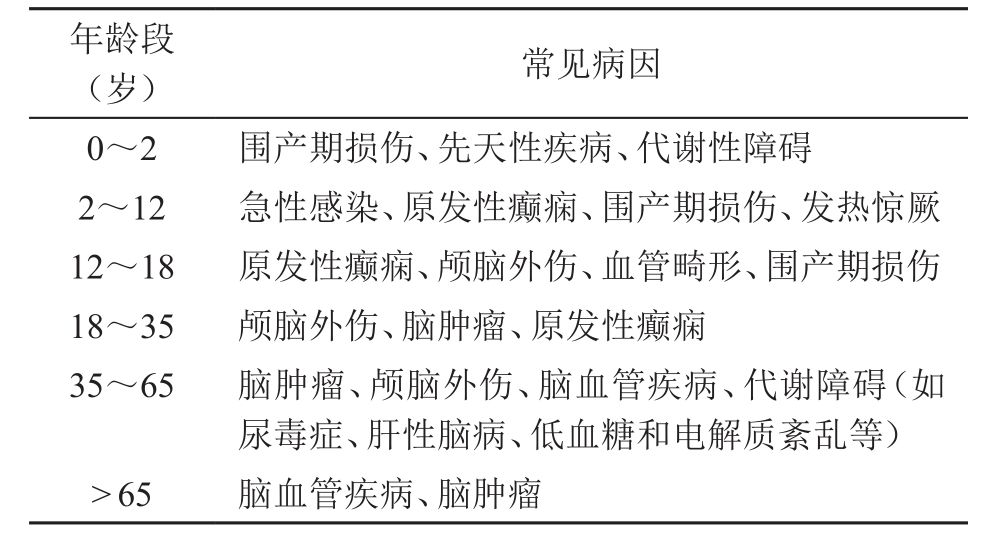
\includegraphics[width=3.27083in,height=1.78125in]{./images/Image00384.jpg}
\end{table}

癫痫持续状态最常见的原因是不恰当地停用抗癫痫药物(antiepileptic
drugs,AEDs)或因急性脑病、脑卒中、脑炎、外伤、肿瘤和药物中毒等引起。不规范AEDs治疗、感染、精神因素、过度疲劳、孕产和饮酒等均可诱发。

\subsubsection{发病机制}

\paragraph{痫性放电的起始}

神经元异常放电是癫痫发病的电生理基础。致痫灶神经元的膜电位与正常神经元不同,在每次动作电位之后出现阵发性去极化漂移(paroxysmal
depolarization
shift,PDS),同时产生高幅高频的棘波放电。神经元异常放电可能由于各种病因导致离子通道蛋白和神经递质或调质异常,出现离子通道结构和功能改变,引起离子异常跨膜运动所致。

\paragraph{痫性放电的传播}

异常高频放电反复通过突触联系和强直后易化作用诱发周边及远处的神经元同步放电,从而引起异常电位的连续传播。异常放电局限于大脑皮质的某一区域时,表现为部分性发作;若异常放电在局部反馈回路中长期传导,表现为部分性发作持续状态;若异常放电不仅波及同侧半球,同时扩散到对侧大脑半球,表现为继发性全面性发作;若异常放电广泛投射至双侧大脑皮质并当网状脊髓束受到抑制时则表现为全身强直-阵挛性发作。

\paragraph{痫性放电的终止}

可能机制是脑内各层结构的主动抑制作用,即癫痫发作时,癫痫灶内产生巨大突触后电位,后者激活负反馈机制,使细胞膜长时间处于过度去极化状态,抑制异常放电扩散,同时减少癫痫灶的传入性冲动,促使发作放电的终止。

癫痫的病因错综复杂,病理改变亦呈多样化,典型改变为海马硬化(hippocampal
sclerosis,HS)。HS肉眼观察表现为海马萎缩、坚硬;组织学表现为双侧HS病变多呈现不对称性,往往发现一侧有明显的HS表现,而另一侧海马仅有轻度的神经元脱失。苔藓纤维出芽(mossy
fiber
sprouting)是HS患者另一重要的病理表现。此外,HS患者还可发现齿状回结构的异常。

\subsection{诊断}

\subsubsection{癫痫发作的分类}

癫痫发作分类是指根据癫痫发作时的临床表现和脑电图(EEG)特征进行分类,目前应用最广泛的是国际抗癫痫联盟(ILAE)1981年癫痫发作分类(表\ref{tab85-2})。2001年ILAE又提出了新的癫痫发作分类(表\ref{tab85-3}),其目的是希望有助于了解癫痫分类学的新观点,并不要求立即用于临床,有待于在临床的使用中不断完善和修改。

\subsubsection{癫痫发作的临床表现特点}

\hypertarget{text00245.htmlux5cux23CHP8-2-2-2-1}{}
(一) 全面性发作

最初的症状学和脑电图提示癫痫全面性发作(generalized
seizures)起源于双侧脑部,多在发作初期就有意识丧失。包括以下类型:

\paragraph{全面强直-阵挛发作(generalized tonic-clonic seizure,GTCS)}

意识丧失、双侧强直后出现阵挛是此型发作的主要临床特征。可由部分性发作演变而来,也可一起病即表现为全面强直-阵挛发作。早期出现意识丧失、跌倒,随后的发作分为三期:①强直期:表现为全身骨骼肌持续性收缩。眼肌收缩出现眼睑上牵、眼球上翻或凝视;咀嚼肌收缩出现张口,随后猛烈闭合,可咬伤舌尖;喉肌和呼吸肌强直性收缩致患者尖叫一声,呼吸停止;颈部和躯干肌肉的强直性收缩致颈和躯干先屈曲,后反张;上肢由上举后旋转为内收旋前,下肢先屈曲后猛烈伸直,持续10~20秒钟后进入阵挛期。②阵挛期:肌肉交替性收缩与松弛,呈一张一弛交替性抽动,阵挛频率逐渐变慢,松弛时间逐渐延长,本期可持续30~60秒钟或更长。在一次剧烈阵挛后,发作停止,进入发作后期。以上两期均可发生舌咬伤,并伴呼吸停止、血压升高、心率加快、瞳孔散大、光反射消失、唾液和其他分泌物增多;Babinski征可为阳性。③发作后期:此期尚有短暂阵挛,以面肌和咬肌为主,导致牙关紧闭,可发生舌咬伤。本期全身肌肉松弛,括约肌松弛,尿液自行流出可发生尿失禁。呼吸首先恢复,随后瞳孔、血压、心率渐至正常。肌张力松弛,意识逐渐恢复。从发作到意识恢复约历时5~15分钟。患者醒后常感头痛、全身酸痛、瞌睡,部分患者有意识模糊,此时强行约束患者可能发生伤人和自伤。GTCS典型EEG改变是,强直期开始逐渐增强的10次/秒棘波样节律,然后频率不断降低,波幅不断增高,阵挛期弥漫性慢波伴间歇性棘波,痉挛后期呈明显脑电抑制,发作时间愈长,抑制愈明显。

\begin{table}[htbp]
\centering
\caption{1981年ILAE癫痫发作分类}
\label{tab85-2}
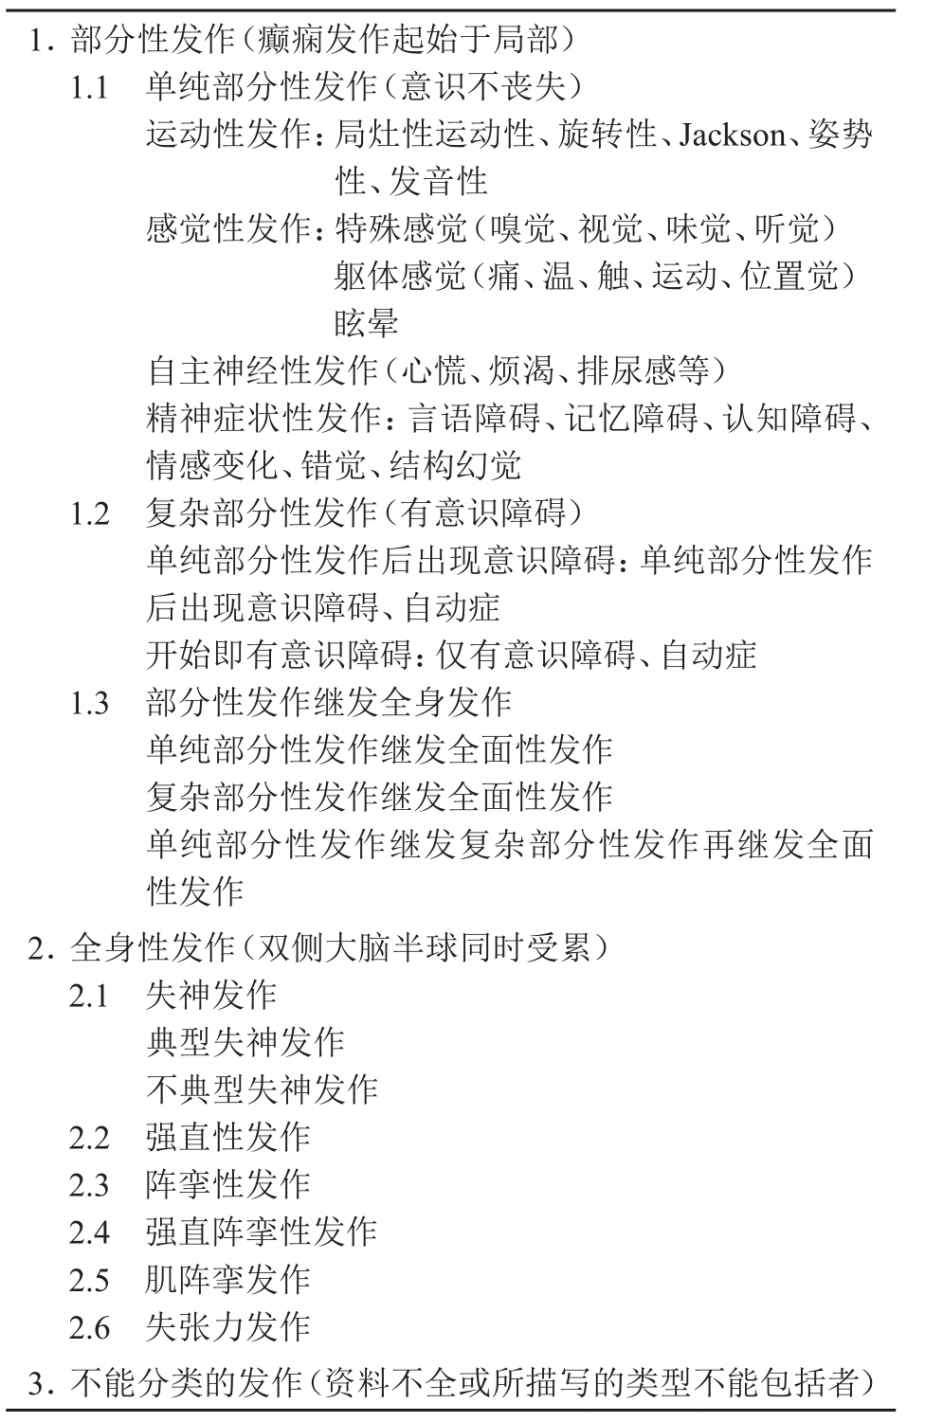
\includegraphics[width=3.25in,height=4.98958in]{./images/Image00385.jpg}
\end{table}

\paragraph{强直性发作(tonic seizure)}

多见于弥漫性脑损伤的儿童,睡眠中发作较多。表现为与强直-阵挛性发作中强直期相似的全身骨骼肌强直性收缩,常伴有明显的自主神经症状,如面色苍白等,如发作时处于站立位可剧烈摔倒。发作持续数秒至数十秒。典型发作期EEG为暴发性多棘波。

\begin{table}[htbp]
\centering
\caption{2001年ILAE癫痫发作的分类}
\label{tab85-3}
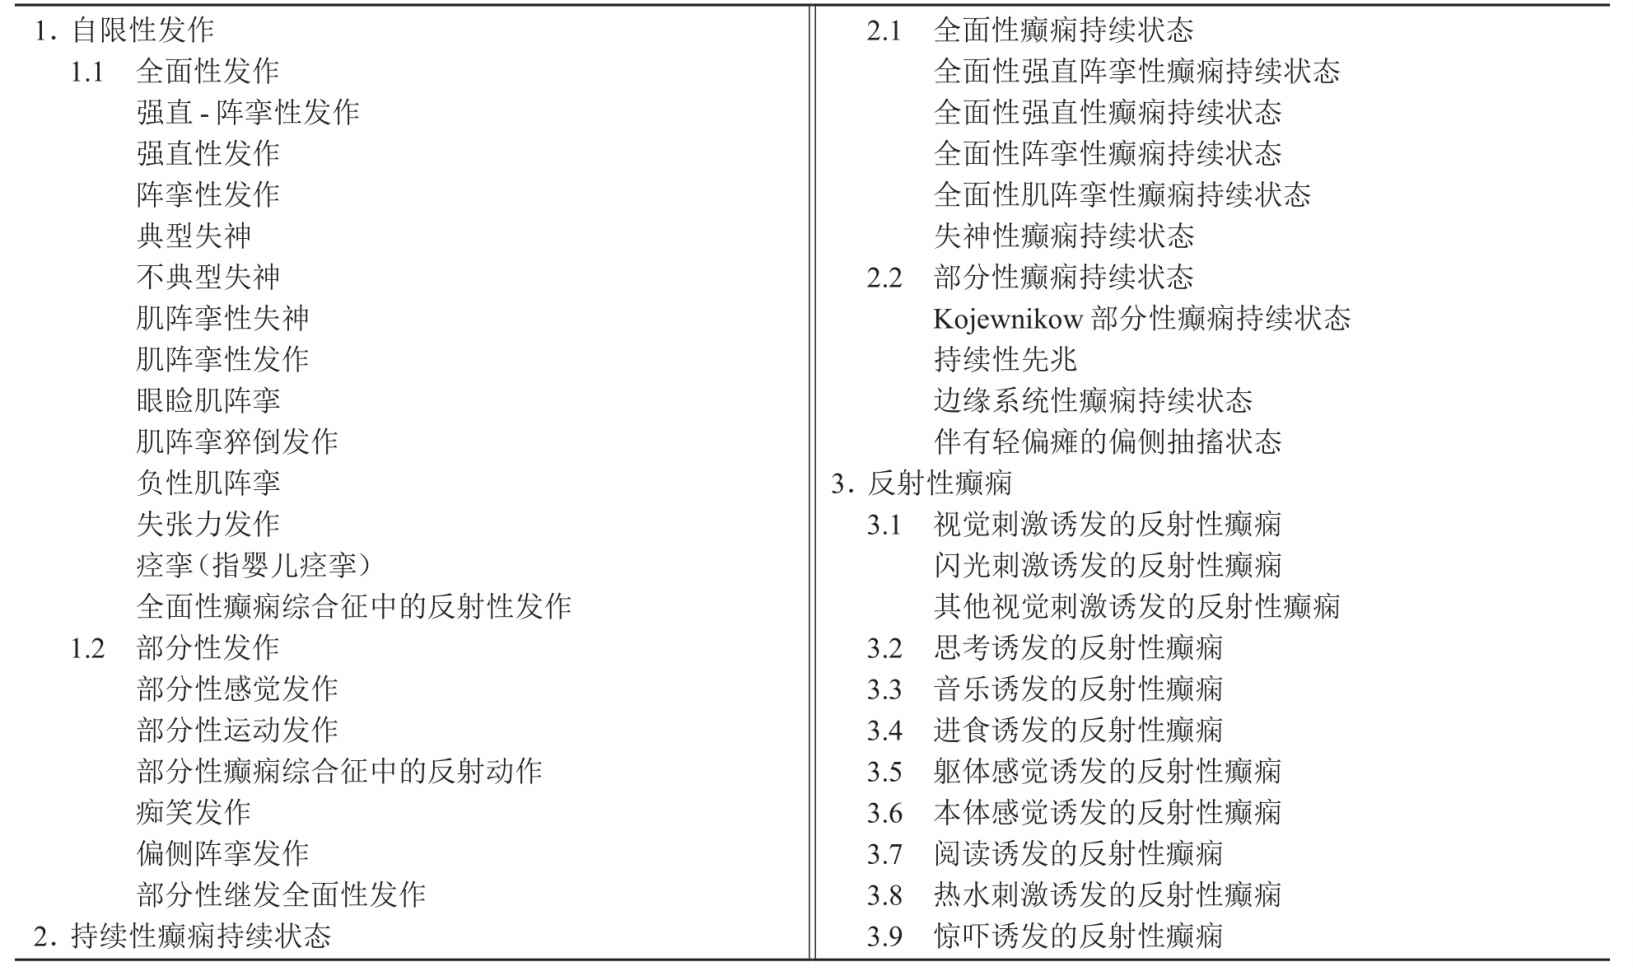
\includegraphics[width=6.60417in,height=3.9375in]{./images/Image00386.jpg}
\end{table}

\paragraph{阵挛性发作(clonic seizure)}

几乎都发生在婴幼儿,特征是重复阵挛性抽动伴意识丧失,之前无强直期。双侧对称或某一肢体为主的抽动,幅度、频率和分布多变,为婴儿发作的特征,持续1分钟至数分钟。EEG缺乏特异性,可见快活动、慢波及不规则棘-慢波等。

\paragraph{失神发作(absence seizure)}

分典型和不典型失神发作,临床表现、EEG背景活动及发作期改变、预后等均有较大差异。①典型失神发作:儿童期起病,青春期前停止发作。特征性表现是突然短暂的(5~10秒)意识丧失和正在进行的动作中断,双眼茫然凝视,呼之不应,可伴简单自动性动作,如擦鼻、咀嚼、吞咽等,或伴失张力如手中持物坠落或轻微阵挛,一般不会跌倒,事后对发作全无记忆,每日可发作数次至数百次。发作后立即清醒,无明显不适,可继续先前活动。醒后不能回忆。发作时EEG呈双侧对称3Hz棘-慢综合波。②不典型失神发作:起始和终止均较典型失神缓慢,除意识丧失外,常伴肌张力降低,偶有肌阵挛。EEG显示较慢的(2.0~2.5Hz)不规则棘-慢波或尖-慢波,背景活动异常。多见于有弥漫性脑损害患儿,预后较差。

\paragraph{肌阵挛发作(myoclonic seizure)}

表现为快速、短暂、触电样肌肉收缩,可遍及全身,也可限于某个肌群或某个肢体,常成簇发生,声、光等刺激可诱发。可见于任何年龄,常见于预后较好的原发性癫痫患者,如婴儿良性肌阵挛性癫痫;也可见于罕见的遗传性神经变性病以及弥漫性脑损害。发作期典型EEG改变为多棘-慢波。

\paragraph{失张力发作(atonic seizure)}

是姿势性张力丧失所致。部分或全身肌肉张力突然降低导致垂颈(点头)、张口、肢体下垂(持物坠落)或躯干失张力跌倒或猝倒发作,持续数秒钟至1分钟,时间短者意识障碍可不明显,发作后立即清醒和站起。EEG示多棘-慢波或低电位活动。

\hypertarget{text00245.htmlux5cux23CHP8-2-2-2-2}{}
(二) 部分性发作

癫痫部分性发作(partial
seizures)是指源于大脑半球局部神经元异常放电,包括单纯部分性、复杂部分性、部分性继发全面性发作三类,前者为局部性发放,无意识障碍,后两者放电从局部扩展到双侧脑部,出现意识障碍。

\paragraph{单纯部分性发作(simple partial seizure)}

发作时程短,一般不超过1分钟,发作起始与结束均较突然,无意识障碍。可分为以下四型:

\hypertarget{text00245.htmlux5cux23CHP8-2-2-2-2-1-1}{}
(1) 部分运动性发作:

表现为身体某一局部发生不自主抽动,多见于一侧眼睑、口角、手或足趾,也可波及一侧面部或肢体,病灶多在中央前回及附近。常见以下几种发作形式:①Jackson发作:异常运动从局部开始,沿大脑皮质运动区移动,临床表现抽搐自手指-腕部-前臂-肘-肩-口角-面部逐渐发展,称为Jackson发作;严重部分运动性发作患者发作后可留下短暂性(0.5~36小时内消除)肢体瘫痪,称为Todd麻痹;②旋转性发作:表现为双眼突然向一侧偏斜,继之头部不自主同向转动,伴有身体的扭转,但很少超过180°,部分患者过度旋转可引起跌倒,出现继发性全面性发作;③姿势性发作:表现为发作性一侧上肢外展、肘部屈曲、头向同侧扭转、眼睛注视着同侧;④发音性发作:表现为不自主重复发作前的单音或单词,偶可有语言抑制。

\hypertarget{text00245.htmlux5cux23CHP8-2-2-2-2-1-2}{}
(2) 部分感觉性发作:

躯体感觉性发作常表现为一侧肢体麻木感和针刺感,多发生在口角、舌、手指或足趾,病灶多在中央后回躯体感觉区;特殊感觉性发作可表现为视觉性(如闪光或黑矇等)、听觉性、嗅觉性和味觉性;眩晕性发作表现为坠落感、飘动感或水平/垂直运动感等。

\hypertarget{text00245.htmlux5cux23CHP8-2-2-2-2-1-3}{}
(3) 自主神经性发作:

出现苍白、面部及全身潮红、多汗、立毛、瞳孔散大、呕吐、腹痛、肠鸣、烦渴和排尿感等。病灶多位于岛叶、丘脑及周围(边缘系统),易扩散出现意识障碍,成为复杂部分性发作的一部分。

\hypertarget{text00245.htmlux5cux23CHP8-2-2-2-2-1-4}{}
(4) 精神性发作:

可表现为各种类型的记忆障碍(如似曾相识、似不相识、强迫思维、快速回顾往事)、情感障碍(无名恐惧、忧郁、欣快、愤怒)、错觉(视物变形、变大、变小,声音变强或变弱)、复杂幻觉等。常为复杂部分性发作的先兆,也可继发全面性强直-阵挛发作。

\paragraph{复杂部分性发作(complex partial seizure,CPS)}

占成人癫痫发作的50\%以上,也称为精神运动性发作,病灶多在颞叶。临床表现有较大差异,主要分以下类型:①仅表现为意识障碍。②表现为意识障碍和自动症:经典的CPS可从先兆开始,以上腹部异常感觉最常见,也可出现情感(恐惧)、认知(似曾相识)和感觉性(嗅幻觉)症状,随后出现意识障碍、呆视和动作停止,发作通常持续1~3分钟。自动症是指在癫痫发作过程中或发作后意识模糊状态下出现的具有一定协调性和适应性的无意识活动。自动症可表现为反复咂嘴、撅嘴、咀嚼、舔舌、牙或吞咽(口、消化道自动症);或反复搓手、拂面,不断地穿衣、脱衣、解衣扣、摸索衣服(手足自动症);也可表现为游走、奔跑、无目的的开门、关门、乘车上船;还可出现自言自语、叫喊、唱歌(语言自动症)或机械重复原来的动作。③表现为意识障碍与运动症状:运动症状可为局灶性或不对称强直、阵挛和变异性肌张力动作,各种特殊姿势(如击剑样动作)等。

\paragraph{部分性发作继发全面性发作}

单纯部分性发作可发展为复杂部分性发作,单纯或复杂部分性发作均可泛化为全面性强直阵挛发作。

\paragraph{痴笑发作}

没有诱因的、刻板的、反复发作的痴笑,常伴有其他癫痫表现,发作期和发作间期EEG有痫样放电,无其他疾病能解释这种发作性痴笑。痴笑是这种发作的主要特点,也可以哭为主要表现。

\subsubsection{癫痫持续状态的临床表现特点}

\hypertarget{text00245.htmlux5cux23CHP8-2-2-3-1}{}
(一) 全面性发作持续状态

\paragraph{全面性强直 -阵挛发作持续状态}

是最常见、最严重的持续状态类型。是以反复发生强直-阵挛性抽搐为特征,二次发作间歇患者意识不恢复,处于昏迷状态。患者同时伴有心动过速,呼吸加快,血压改变,发热,酸中毒,腺体分泌增多(可致呼吸道阻塞)等全身改变。

\paragraph{强直性发作持续状态}

主要见于Lennox-Gastaut综合征患儿,表现不同程度意识障碍(昏迷较少),间有强直性发作或其他类型发作,如肌阵挛、非典型失神、失张力发作等。EEG出现持续性较慢的棘-慢或尖-慢波放电。

\paragraph{阵挛性发作持续状态}

阵挛性发作持续状态时间较长时可出现意识模糊甚至昏迷。

\paragraph{肌阵挛发作持续状态}

特发性肌阵挛发作患者很少出现癫痫状态,严重器质性脑病晚期如亚急性硬化性全脑炎、家族性进行性肌阵挛癫痫等较常见。

\paragraph{失神发作持续状态}

主要表现为意识水平降低,甚至只表现反应性低下,学习成绩下降。EEG可见持续性棘-慢波放电,频率较慢(<
3Hz)。

\hypertarget{text00245.htmlux5cux23CHP8-2-2-3-2}{}
(二) 部分性发作持续状态

\paragraph{单纯部分性发作持续状态}

临床表现以反复的局部颜面或躯体持续抽搐为特征,或持续的躯体局部感觉异常为特点,发作时意识清楚,EEG上有相应脑区局限性放电。

\paragraph{边缘叶性癫痫持续状态}

常表现为意识障碍和精神症状,又称精神运动性癫痫状态,常见于颞叶癫痫。

\paragraph{偏侧抽搐状态伴偏侧轻瘫}

多发生于幼儿,表现一侧抽搐,伴发作后一过性或永久性同侧肢体瘫痪。

\subsubsection{辅助检查}

\paragraph{脑电图(EEG)}

是诊断癫痫最重要的辅助检查方法。常规头皮EEG仅能记录到49.5\%患者的痫性放电,采用过度换气、闪光刺激等诱导方法虽可提高EEG阳性率,但仍有部分患者的EEG检查始终正常。部分正常人中偶尔也可记录到痫性放电,因此不能单纯依据EEG检查来确定是否为癫痫。24小时长程脑电监测使发现痫性放电的阳性率大为提高,而视频脑电图(video-EEG)可同步监测记录患者发作情况及相应EEG改变,明确发作性症状与EEG变化间的关系。

\paragraph{神经影像学检查}

包括头颅CT和MRI,可确定脑结构异常或病变。ILAE神经影像学委员会(1997年)制订的神经影像学检查指征是:①任何年龄、病史或EEG说明为部分性发作;②在1岁以内或成人未能分型的发作或明显的全面性发作;③神经或神经心理证明有局限性损害;④一线AEDs无法控制发作;⑤AEDs不能控制发作或发作类型有变化以及可能有进行性病变者。功能影像学检查如SPECT、PET等能从不同的角度反映脑局部代谢变化,辅助癫痫灶的定位。

\subsubsection{诊断注意事项}

癫痫的诊断需遵循三步原则:首先明确发作性症状是否为癫痫发作;其次是明确哪种类型的癫痫或癫痫综合征;最后明确发作的病因是什么。

\paragraph{癫痫诊断的确立}

癫痫是发作障碍性疾病,但很多发作障碍性疾病并不是癫痫,如睡眠障碍性疾病中的夜游症,常需与复杂部分性癫痫发作鉴别。短暂性脑缺血发作、晕厥、偏头痛、眩晕及癔症等均为发作性疾患。因此应通过详细的病史及有关的实验室检查,与上述等疾病鉴别,确立或排除癫痫的诊断。需强调的是:诊断癫痫发作最重要的依据是患者的病史,如先兆症状、发作时状态及发作后意识模糊等,而不是依靠神经系统检查和实验室检查;患者发作后意识模糊状态高度提示癫痫发作,躯体抽动和尿失禁并不一定提示痫性发作,因也可能发生于血管迷走性晕厥及其他原因的晕厥。

\paragraph{癫痫发作类型的诊断}

不同的癫痫发作类型,对药物反应不同,从治疗的角度出发,发作类型诊断是十分重要的。详细询问患者及亲属、目击者,患者发作时,是否伴有意识障碍,有无先兆,发作时的具体表现,以及既往史和家族史等,对于发作类型的诊断是至关重要的。EEG在癫痫及癫痫发作类型的诊断中是必不可少的技术。

\paragraph{病因诊断}

对症状性癫痫要查明原因。详细的病史,常可提供病因的线索(如产伤、头部外伤、脑膜炎、脑炎、脑卒中等)。疑有脑寄生虫病患者,应进行大便寄生虫卵、绦虫节片及血液、脑脊液的囊虫补体或血凝试验。疑是颅内占位病变、先天发育异常或原因不明者,应进行头部X线平片、头颅CT及MRI检查。怀疑有脑血管畸形的患者,需做MRA或脑血管造影。不要忽视全身性疾病的因素,如低血钙、低血糖、肾衰等全身代谢障碍及系统性红斑狼疮等全身疾病引起的脑损害。

\subsection{治疗}

\subsubsection{病因治疗}

如治疗急、慢性中枢神经系统感染,纠正及治疗代谢障碍,切除颅内肿瘤等。在切除脑膜瘤后,仅仅50\%病例癫痫发作缓解,胶质瘤缓解的百分比甚至更低,因此这样的病例,应继续药物治疗。

\subsubsection{药物治疗}

药物治疗是癫痫治疗的主要手段。药物治疗应达到三个目的:控制发作或最大限度地减少发作次数;长期治疗无明显的不良反应;使患者保持或恢复其原有的生理、心理和社会功能状态。大约2/3的患者,应用抗癫痫药治疗后,发作获满意控制,20\%~25\%的病例发作频率及严重性明显减少或减轻。

药物治疗的一般原则如下:

\paragraph{确定是否用药}

人一生中偶发一至数次癫痫的概率高达5\%,且39\%癫痫患者有自发性缓解倾向,并非每个癫痫患者都需要用药。用药指征:①半年内发作两次以上者;②首次发作或间隔半年以上发作一次者,可在告知AEDs可能的不良反应和不经治疗的可能后果的情况下,依患者及家属的意愿用或不用AEDs。

\paragraph{正确选择药物}

应根据癫痫发作类型、癫痫及癫痫综合征类型选择用药。2006年ILAE推出针对不同发作类型癫痫的治疗指南见表\ref{tab85-4},在实际工作中需结合医生的经验及患者的反应来选择药物。

\paragraph{尽可能单药治疗}

70\%~80\%的癫痫患者可以通过单药治疗控制发作。单药治疗应从小剂量开始,缓慢增量至能最大程度地控制癫痫发作而无不良反应或很轻,即为最低有效剂量;若不能有效控制癫痫发作,则满足部分控制,也不能出现不良反应。监测血药浓度以指导用药。常用的传统AEDs有苯妥英钠(phenytoin)、卡马西平(carbamazepine)、丙戊酸(valproate)、苯巴比妥(phenobarbital)、扑痫酮(primidone)、乙琥胺(ethosuximide)和氯硝西泮(clonazepam)等;新型AEDs有托吡酯(topiramate,妥泰)、拉莫三嗪(lamotrigine)、加巴喷丁(gabapentin)、非尔氨酯(felbamate)、噻加宾(tiagabine,替加平)、氨己烯酸(vigabatrin,喜保宁)、奥卡西平(oxcarbazepine,确乐多)和左乙拉西坦(levetiracetam)等。

\paragraph{用药方法}

用药方法取决于药物代谢特点、作用原理及不良反应出现规律等,差异很大。如苯妥英钠常规剂量无效时增加剂量极易中毒;丙戊酸治疗范围大,开始可用常规剂量;卡马西平因自身诱导作用使代谢逐渐加快,半衰期缩短,需逐渐加量,约一周达到常规剂量。拉莫三嗪、托吡酯应逐渐加量,约一个月达治疗剂量,否则易出现皮疹、CNS不良反应等。应坚持不间断及有规律地服药,以保证血药浓度处于有效治疗范围内,根据药物的半衰期决定服药次数(表\ref{tab85-5})。

\paragraph{严密观察不良反应}

AEDs的不良反应包括特异性、剂量相关性、慢性及致畸性(表\ref{tab85-6}),以剂量相关性不良反应最常见,通常发生于用药初始和增量时,与血药浓度有关。多数常见的不良反应为短暂性的,缓慢减量即可明显减少。应用AEDs前应检查肝肾功能和血尿常规,用药后每月监测血尿常规,每季度监测肝肾功能,至少持续半年。多数AEDs为碱性,饭后服药可减轻胃肠道反应。应用AEDs可能发生急性过敏反应,所有的过敏反应均应立即停药。

\paragraph{合理的联合治疗}

合理的多药联合治疗是指“在最小程度增加不良反应的前提下,获得最大程度的发作控制”。约20\%的患者在两种单药治疗后仍不能控制发作,应考虑合理的联合治疗。指征:①单药治疗无效的患者;②有多种类型的发作;③针对药物的不良反应,如苯妥英钠治疗部分性发作时出现失神发作,除选用广谱AEDs外,也可合用氯硝西泮治疗苯妥英钠引起的失神发作;④针对患者的特殊情况,如月经性癫痫患者可在月经前后加用乙酰唑胺,以提高疗效。注意事项:①不宜合用化学结构相同的药物,如苯巴比妥与扑痫酮,氯硝西泮和地西泮;②尽量避开副作用相同的药物合用,如苯妥英钠可引起肝肾损伤,丙戊酸可引起特异过敏性肝坏死;③合用药物时要注意药物的相互作用。

\begin{table}[htbp]
\centering
\caption{国际抗癫痫联盟推荐的用药方案(ILAE治疗指南2006)}
\label{tab85-4}
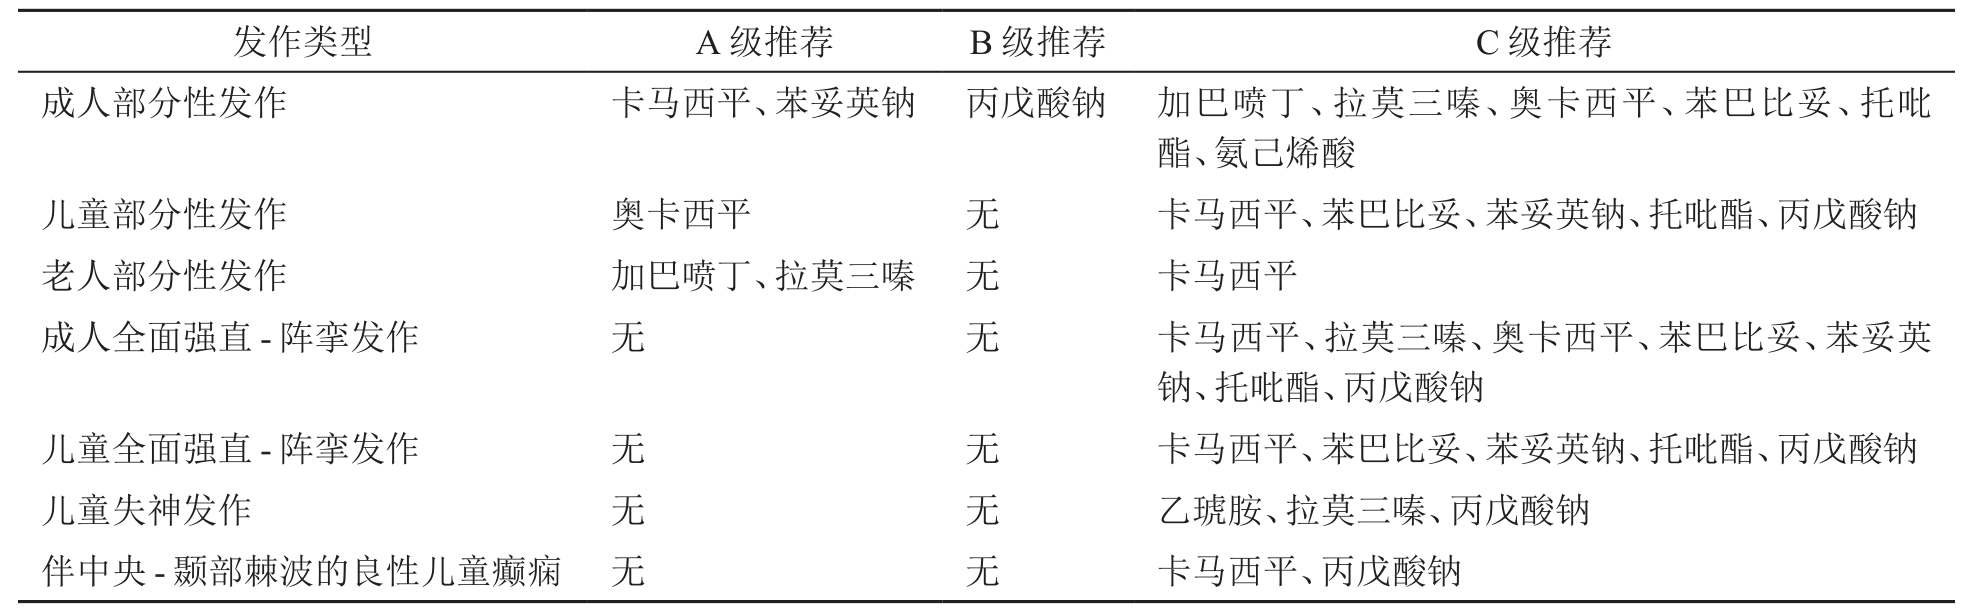
\includegraphics[width=6.57292in,height=2.03125in]{./images/Image00387.jpg}
\end{table}

\begin{table}[htbp]
\centering
\caption{抗癫痫药物的药代动力学和剂量}
\label{tab85-5}
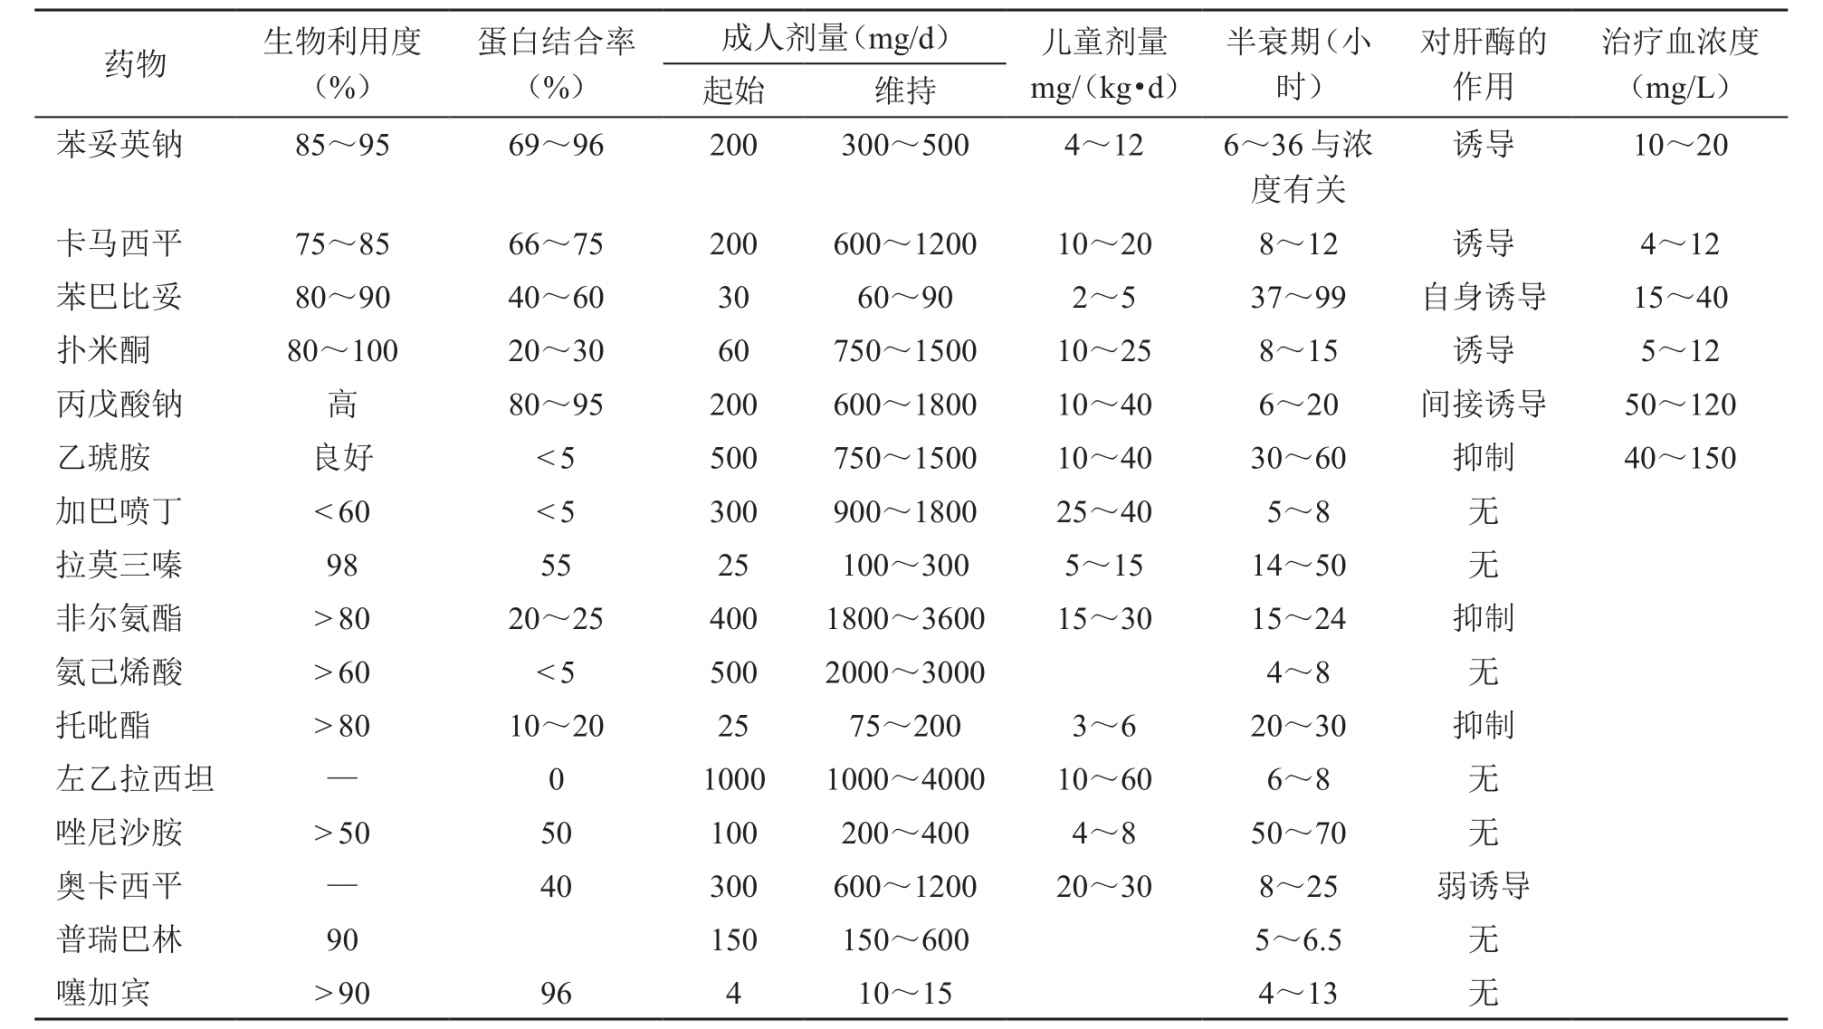
\includegraphics[width=6.70833in,height=3.78125in]{./images/Image00388.jpg}
\end{table}

\begin{table}[htbp]
\centering
\caption{抗癫痫药物的不良反应}
\label{tab85-6}
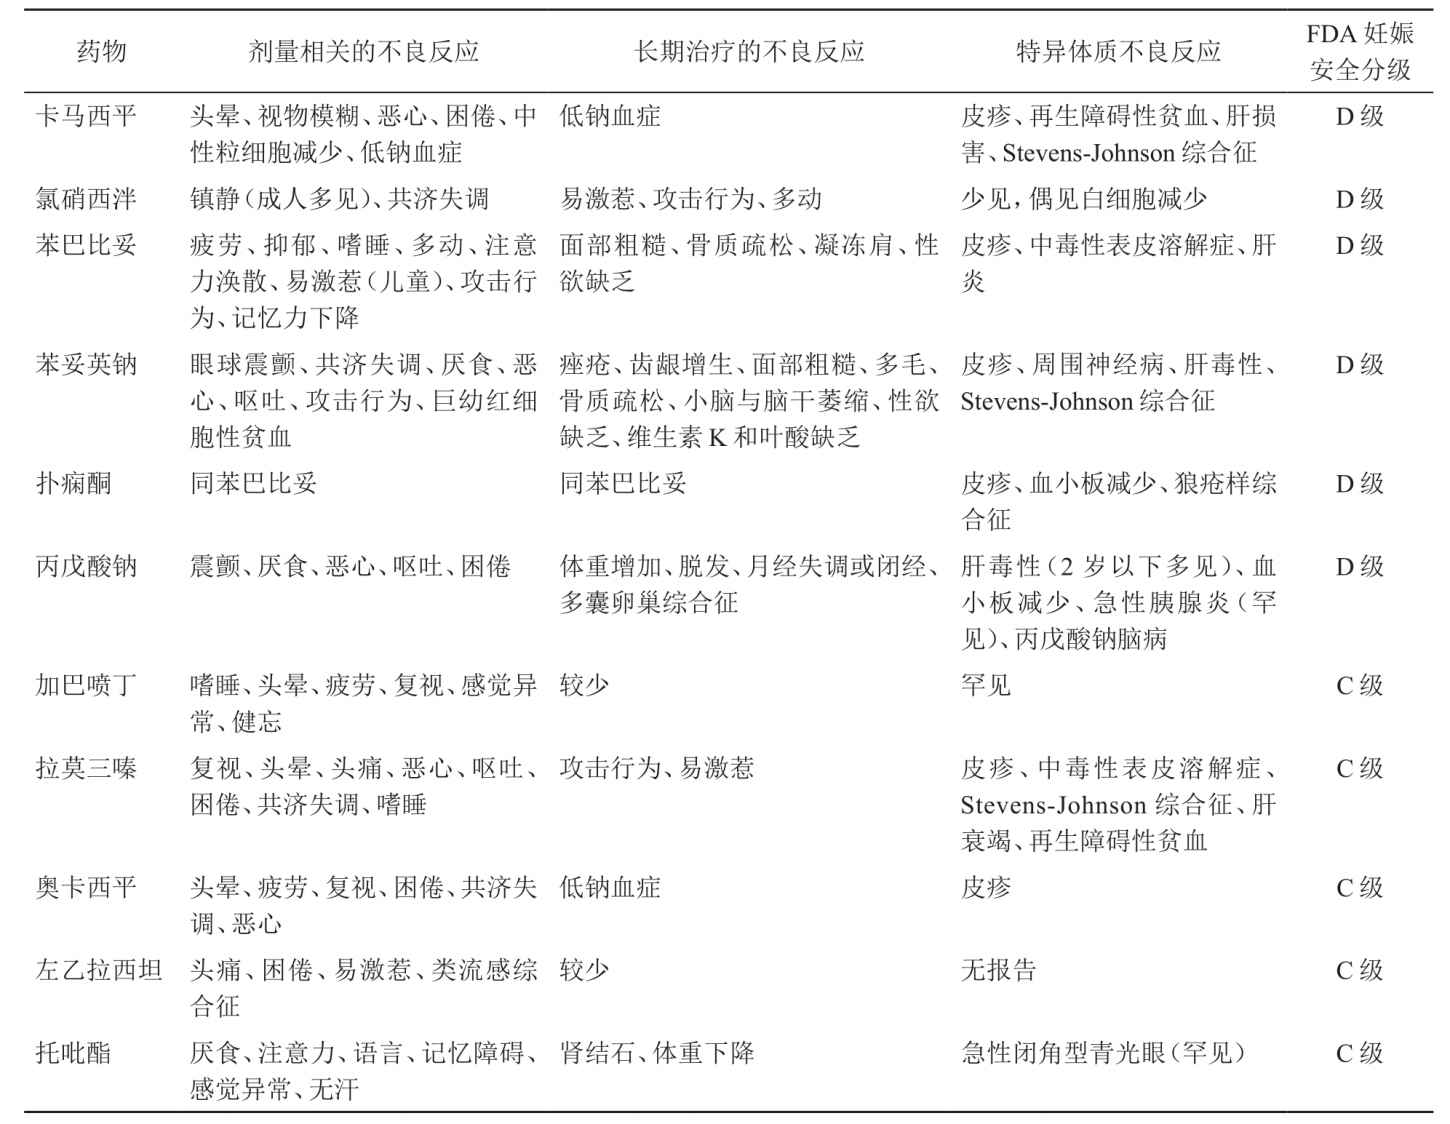
\includegraphics[width=6.63542in,height=5.14583in]{./images/Image00389.jpg}
\end{table}

\paragraph{增减药物、停药及换药原则}

①增减药物:增药可适当快些,减药一定要慢,必须逐一增减,以利于确切评估疗效和毒副作用;②AEDs控制发作后必须坚持长期服用,不宜随意减量或停药,以免诱发癫痫持续状态,除非出现严重的不良反应;③换药:若一种一线药物已达到最大可耐受剂量依然不能控制发作,可加用另一种一线或二线药物,至发作控制或达到最大可耐受剂量后逐渐减掉原有的药物,转换为单药。换药期间应有5~7天的过渡期;④停药:全面强直-阵挛性发作、强直性发作、阵挛性发作完全控制4~5年后,失神发作停止半年后可考虑停药,但停药前应有缓慢减量的过程,一般不少于1~1.5年无发作者方可停药。

20\%~30\%复杂部分性发作患者用各种AEDs治疗难以控制发作,如治疗2年以上,血药浓度在正常范围内,每月仍有4次以上发作称为难治性癫痫(intractable
epilepsy)。

\subsubsection{手术治疗}

患者经过长时间正规单药治疗,或先后用两种AEDs达到最大耐受剂量,以及经过一次正规的、联合治疗仍不见效,可考虑手术治疗。手术适应证主要是起源于一侧颞叶的难治性复杂部分性发作,如致痫灶靠近大脑皮质、可为手术所及且切除后不会产生严重的神经功能缺陷,疗效较好。常用的方法有前颞叶切除术、颞叶以外的脑皮质切除术、癫痫病灶切除术、大脑半球切除术、胼胝体切开术等。

\subsubsection{癫痫持续状态的治疗}

癫痫持续状态的治疗目的是:保持稳定的生命体征进行心肺功能支持;终止呈持续状态的癫痫发作,减少癫痫发作对脑部神经元的损害;寻找并尽可能根除病因与诱因;防治并发症。

\paragraph{一般治疗}

①防止缺氧和损伤:应立即使患者侧卧,尽量让唾液和呕吐物流出口外,保持呼吸道通畅,吸痰、吸氧,必要时气管插管或切开。在患者张口时,可将折叠成条状的小毛巾、手帕或牙套等塞入上下臼齿之间,以免舌部咬伤。抽搐时不可用力按压患者的身体,以免造成骨折。亦不要采取所谓掐“人中”的方法,因为此举不仅不能制止发作,反有可能对患者造成新的伤害。尽可能对患者进行心电、血压、呼吸、脑电的监测。②迅速进行神经系统及心肺功能检查及有关实验室检查:如血药浓度、血糖、肾功能、电解质、测定动脉血pH、氧及二氧化碳分压,及时纠正合并的全身性改变。③呼吸稳定后,应查明原因,如断药、低血糖、中毒、感染等,以便针对病因治疗。④静脉注射50\%葡萄糖,预防低血糖,之后以生理盐水或葡萄糖维持。⑤治疗脑水肿:常用20\%甘露醇125~250ml静滴。

\paragraph{尽快终止癫痫状态}

应选择速效、抗痫力强、安全、对心肺无抑制作用的药物。

\hypertarget{text00245.htmlux5cux23CHP8-2-3-4-2-1}{}
(1) 地西泮:

首选药物。成人10~20mg/次,儿童0.25~0.5mg/kg。缓慢静脉注射(成人应小于5mg/min,儿童2mg/min),直到发作停止。10~15分钟后可重复给药,24小时总量不得超过200mg。也可在首次静脉注射后,如有效,可用地西泮60~100mg加入生理盐水(或5\%葡萄糖液)500ml中于12小时内缓慢静脉滴注。

\hypertarget{text00245.htmlux5cux23CHP8-2-3-4-2-2}{}
(2) 地西泮加苯妥英钠:

首先用地西泮10~20mg静注取得疗效后,再用苯妥英钠0.3~0.6g加入生理盐水250~500ml中静滴,速度不超过50mg/min。用药中如出现血压降低或心律不齐时需减缓静滴速度或停药。

\hypertarget{text00245.htmlux5cux23CHP8-2-3-4-2-3}{}
(3) 苯妥英钠:

部分患者也可单用苯妥英钠。成人首次剂量500~750mg,儿童10~15mg/kg,以生理盐水作溶剂,静脉注射速度不超过50mg/min,以避免发生低血压、心律失常。抽搐停止后,每6~8小时口服或静脉注射50~100mg的维持量。其优点是无呼吸抑制及镇静作用,便于意识状态的观察。

\hypertarget{text00245.htmlux5cux23CHP8-2-3-4-2-4}{}
(4) 氯硝西泮:

起效快,药效是地西泮的5倍,维持时间比地西泮长1~2倍。一般成人首次用1~4mg、儿童0.02~0.06mg/kg缓慢静脉注射,20分钟后可重复原剂量2次,兴奋躁动者可适当加大剂量。

\hypertarget{text00245.htmlux5cux23CHP8-2-3-4-2-5}{}
(5) 10\%水合氯醛:

20~30ml加等量植物油保留灌肠,8~12小时一次。适合肝功能不全或不宜使用苯巴比妥类药物者。

\hypertarget{text00245.htmlux5cux23CHP8-2-3-4-2-6}{}
(6) 副醛:

8~10ml(儿童0.3ml/kg)植物油稀释后保留灌肠。可引起剧咳,有呼吸疾病者勿用。

经上述处理,发作控制后,可用苯巴比妥0.1~0.2g肌注,每日2次,巩固和维持疗效。同时鼻饲AEDs,达稳态浓度后逐渐停用苯巴比妥。上述方法无效者,需按难治性癫痫持续状态处理。

\paragraph{难治性癫痫持续状态的处理}

难治性癫痫持续状态是指持续的癫痫发作,对初期的一线药物地西泮、氯硝西泮、苯巴比妥、苯妥英钠等无效,连续发作1小时以上者。对难治性癫痫持续状态的首要任务是迅速终止发作,可选用以下药物:

\hypertarget{text00245.htmlux5cux23CHP8-2-3-4-3-1}{}
(1) 异戊巴比妥钠(阿米妥钠):

是治疗难治性癫痫持续状态的标准疗法。成人0.25~0.5g/次溶于注射用水10ml静脉注射,儿童1~4岁0.1g/次,5岁以上0.2g/次,速度不超过0.05g/min,至控制发作为止。低血压、呼吸抑制、复苏延迟是其主要的不良反应,在使用中常需行气管插管,机械通气来保证生命体征的稳定。

\hypertarget{text00245.htmlux5cux23CHP8-2-3-4-3-2}{}
(2) 咪达唑仑:

常用剂量为首剂静注0.15~0.2mg/kg,然后按0.06~0.6mg/(kg•h)静滴维持。新生儿可按0.1~0.4mg/(kg•h)静滴维持。因起效快,对血压和呼吸抑制作用较小,已有取代异戊巴比妥钠的趋势。

\hypertarget{text00245.htmlux5cux23CHP8-2-3-4-3-3}{}
(3) 丙泊酚(propofol,异丙酚):

是一种非巴比妥类的短效静脉用麻醉剂,能明显增强GABA能神经递质的释放,可在几秒钟内终止癫痫发作和EEG上的痫性放电,平均起效时间2.6分钟。建议剂量1~2mg/kg静注,继以2~10mg/(kg•h)静滴维持。突然停用可致发作加重,逐渐减量则不出现癫痫发作的反跳。

\hypertarget{text00245.htmlux5cux23CHP8-2-3-4-3-4}{}
(4) 利多卡因:

对苯巴比妥治疗无效的新生儿癫痫持续状态有效,终止发作的首次负荷量为1~3mg/kg静脉注射,速度<
25~50mg/min。然后用2~4mg/(kg•h),静脉滴注1~3天。在应用利多卡因时应注意其常见的不良反应,如烦躁、谵妄、精神异常、心律失常及过敏反应等。心脏传导阻滞及心动过缓者慎用。应用时应监测心脏。

\hypertarget{text00245.htmlux5cux23CHP8-2-3-4-3-5}{}
(5) 其他药物:

可酌情选择使用:①氯胺酮(ketamine):为非巴比妥类的短效静脉麻醉剂,成人建议剂量1~2mg/kg静注。②硫喷妥钠:为超短时作用的巴比妥类药物,成人建议剂量0.05~0.1g。

\subsubsection{一般及精神心理卫生}

睡眠减少、饮酒及其他药物的滥用常是癫痫发作突然增多的重要原因,因此患者应保持一定的睡眠时间,节制饮酒,在医生指导下用药。要有良好的饮食习惯,避免暴饮暴食,养成大便习惯,如需要可应用缓泻剂。避免高空水上作业,以免发作时造成危险。癫痫是慢性病,绝大多数患者需长期服用抗癫痫药控制发作及适应慢性病的生活方式,要帮助癫痫患者克服自卑感,亲友及周围同志不要过分的关心及过分的保护,要让患者正常的生活、工作及学习,鼓励患者进行适量的体育锻炼。

癫痫系慢性疾病,其预后与诸多因素有关,如病因、发病年龄、发作类型、频率、脑电图改变等,一般认为,发病年龄早、发作频繁、有精神智能缺陷、颅内有器质性疾患、脑电图异常者及一些特殊的综合征(如Lennox-Gastaut综合征、婴儿痉挛等)预后较差。除癫痫持续状态外,很少引起死亡,除非发作时出现意外事故。

\protect\hypertarget{text00246.html}{}{}

\hypertarget{text00246.htmlux5cux23CHP8-2-4}{}
参 考 文 献

1. 贾建平.神经病学.第6版.北京:人民卫生出版社,2008:292-315

2. LaRoche SM,Helmers SL. The new antiepileptic drugs:scientific
review. JAMA,2004,291(5):605

3. 陈灏珠 ,林果为.实用内科学.第13版.北京:人民卫生出版社,2009:2870

4. Glauser T,Ben-Menachem E,Bourgeois B,et al. ILAE treatment
guidelines:evidence-based analysis of antiepileptic drug efficacy and
effectiveness as initial monotherapy for epileptic seizures and
syndromes. Epilepsia,2006,47:1094-1120

\protect\hypertarget{text00247.html}{}{}

\chapter{脑 膜 炎}

\section{化脓性脑膜炎}

化脓性脑膜炎(purulent
meningitis,简称化脑)是化脓性细菌感染所致的脑脊膜炎症,是中枢神经系统常见的化脓性感染,好发于婴幼儿和儿童。临床上表现为起病急骤,发热、头痛、呕吐、嗜睡、惊厥、意识障碍和脑膜刺激征阳性。

\subsection{病因与发病机制}

化脓性脑膜炎最常见的致病菌为肺炎球菌、脑膜炎球菌和流感嗜血杆菌B型,其次为金黄色葡萄球菌、链球菌、大肠杆菌、变形杆菌、厌氧杆菌、沙门菌、铜绿假单胞菌等。病原菌可通过多种途径侵入脑膜:①由菌血症或败血症经血液循环而到达脑膜;②直接经上呼吸道或颅脑损伤处侵入;③感染病灶如鼻窦炎、中耳炎、乳突炎的扩散或脑脓肿溃破;④脑血管血栓性静脉炎扩散;⑤神经外科手术操作时导入。病原菌一旦在脑膜的任何部位立足,即可迅速波及整个蛛网膜下腔。细菌释放的内毒素或细菌的细胞壁成分刺激局部炎症反应发生化脓性脑膜炎,其发病机制与脑膜炎球菌脑膜炎相似(参见第79章“流行性脑脊髓膜炎”部分)。

各种致病菌引起的急性化脓性脑膜炎的病理变化基本相同。早期软脑膜及大脑浅表血管充血、扩张,炎症沿蛛网膜下腔扩展,大量脓性渗出物覆盖于脑表面,常沉积于脑沟及脑基底部脑池等处,亦可见于脑室内。脓液颜色与致病菌种有关:脑膜炎球菌及金黄色葡萄球菌脓液为灰或黄色;肺炎球菌为淡绿色;流感嗜血杆菌为灰色;大肠杆菌及变形杆菌呈灰黄色;铜绿假单胞菌为草绿色。随着炎症的扩展,浅表软脑膜和室管膜均因纤维蛋白渗出物覆盖而呈颗粒状。病程后期则因脑膜粘连引起脑脊液吸收及循环障碍,导致交通性或非交通性脑积水。儿童病例常出现硬膜下积液、积脓。偶可见静脉窦血栓形成、脑脓肿或因脑动脉内膜炎而致脑软化、梗死。

\subsection{诊断}

\subsubsection{临床表现特点}

\paragraph{共同表现}

各种细菌感染引起的化脑临床表现类似,主要有:①感染症状:发热、寒战或上呼吸道感染表现等。②脑膜刺激征:表现为颈项强直,Kernig征和Brudzinski征阳性。但新生儿、老年人或昏迷者脑膜刺激征常不明显。③颅内压增高:表现为剧烈头痛、呕吐、意识障碍等。④局灶症状:部分患者可出现局灶性神经功能损害的症状,如偏瘫、失语等。

\paragraph{不同年龄的患者化脑临床特点不同}

①新生儿及3个月以下小婴儿化脑:早期临床表现极不典型,可仅表现为拒食、吐奶、嗜睡、凝视、尖叫、惊厥(或仅有面部肌肉小抽动)、呼吸不规则、面色青灰及前囟紧张或隆起等,甚至出现脑膜刺激征或前囟隆起已属化脑晚期。体温可高可低,甚至体温不升。由于新生儿化脑常并发败血症,故可出现黄疸。在新生儿败血症中约1/3病例并发脑膜炎,因此一旦败血症的诊断确立,即应考虑脑膜炎的可能。②3个月~2岁的婴儿化脑:大多有发热、呕吐、烦躁、易激惹、惊厥、精神萎靡、嗜睡或昏迷。颈强直,前囟膨隆,并出现脑膜刺激征。③2岁以上的小儿化脑:症状和体征渐趋典型。年长儿除自述头痛外,尚有背痛、关节肌肉疼痛。脑膜刺激征明显。④成年及老年患者化脑:以肺炎球菌所致化脑多见,其次尚有脑膜炎球菌脑膜炎和革兰阴性杆菌脑膜炎等。

\paragraph{不同病原菌引起的化脑的临床特点}

①脑膜炎球菌脑膜炎:即“流行性脑脊髓膜炎(流脑)”,参见第79章“流行性脑脊髓膜炎”。②肺炎球菌脑膜炎:多见于婴幼儿及老年人,常继发于肺炎、中耳炎、乳突炎、鼻窦炎、败血症或颅脑损伤的耳、鼻漏等患者。冬春季较多。炎症主要分布在大脑顶部的表面,故早期脑膜刺激征可以不明显。脑脊液为脓性,含纤维蛋白较多,常沉积于蛛网膜下腔及大脑表面,形成广泛而较厚的纤维脓性膜,导致粘连和包裹性积脓,使所用治疗药物难以渗入病灶内而致疗效不佳,以致病程迁延和反复再发。硬膜下积液或积脓、脑脓肿、脑积水、脑室梗阻等并发症也较其他化脑多见。病情重,常有意识障碍和昏迷。脑脊液涂片查见肺炎球菌的阳性率可达80\%以上,CSF和血培养也可获阳性结果。③流感嗜血杆菌脑膜炎:多由毒力强的B型流感嗜血杆菌引起,多见于3个月~3岁小儿,高峰易感年龄是7~12个月,占70\%。秋冬季多见。起病时常先有呼吸道炎症,短期内出现嗜睡、易激动或突然尖叫等。偶有皮疹,脑膜刺激征常不典型。CSF呈脓性,涂片可查见革兰染色阴性短小杆菌,阳性率为80\%左右,有早期诊断价值。CSF和血培养分离出流感嗜血杆菌可确诊。常并发硬膜下积液。④葡萄球菌脑膜炎:主要由金黄色葡萄球菌引起。各年龄均可发病,但以新生儿及较大儿童多见。多发生在夏季。常继发于皮肤化脓性感染、各种脓肿、骨髓炎、颅脑手术等,多为金黄色葡萄球菌脓毒血症的迁徙病灶之一。起病急,颈项强直较其他化脑更为显著,常出现瘀点、瘀斑、荨麻疹、猩红热样皮疹及脓疱疹等多种皮疹。体内其他部位也可发现化脓病灶。CSF呈脓性,蛋白含量高,涂片可查见呈簇状排列的革兰染色阳性球菌。CSF或血培养出金黄色葡萄球菌可确诊。⑤大肠杆菌脑膜炎:多见于3个月以内的婴儿,尤其是新生儿和早产儿。此菌主要来自母亲产道或婴儿肠道、脐部。常在出生后1~2周内发病,因前囟未闭,颅内高压和脑膜刺激征可不明显,也不一定有发热,常表现为拒食、嗜睡、烦躁、惊叫、凝视、惊厥和呼吸困难等,CSF可培养出大肠杆菌。预后较差。⑥铜绿假单胞菌脑膜炎:多见于颅脑外伤、压疮感染,或烧伤伴铜绿假单胞菌败血症时,亦可因腰椎穿刺时消毒不严而污染所致。本病进展缓慢,CSF涂片可找到革兰阴性杆菌,确诊有赖于CSF培养出铜绿假单胞菌。⑦厌氧菌脑膜炎:较少见。常为厌氧菌与需氧菌混合感染所致脑脓肿,由于病变局限,故临床表现如发热、全身毒血症症状、脑膜刺激征等不甚明显。

化脓性脑膜炎在病程发展中可发生多种颅内并发症,如硬膜下积液,尤其多见于1岁以下婴儿肺炎球菌和流感嗜血杆菌感染;硬膜下脓肿常见于年轻成年人,通常伴鼻窦炎或耳源性感染,患者常有发热、癫痫发作、局限性神经体征;较少见的有脑脓肿、脑梗死、静脉窦血栓形成、脑室膜炎和脑积水。同时可出现全身性并发症如脓胸、肺脓肿、心内膜炎、化脓性关节炎、肾炎、休克和DIC等。约10\%~20\%的化脑患者可遗留程度不等的智力减退、耳聋、失明、癫痫和瘫痪等。

\subsubsection{辅助检查}

\paragraph{外周血象}

血白细胞计数明显增高,通常为(10~30)× 10\textsuperscript{9}
/L,以中性粒细胞为主。

\paragraph{脑脊液检查}

压力增高,外观混浊或呈脓性,细胞数增多,在(1000~10 000)×
10\textsuperscript{6}
/L,甚至更高,以多形核白细胞为主。有时脓细胞聚集呈块状物,此时细菌培养、涂片阳性率高。蛋白质显著增加,定量在1g/L以上;糖定量降低,通常在2.2mmol/L以下;氯化物降低。CSF中pH降低,乳酸、乳酸脱氢酶(LDH)、溶菌酶的含量以及免疫球蛋白IgG和IgM均明显增高。

\paragraph{其他检查}

每一例化脑均应做血培养。反复再发者应查明原因,可做鼻窦、颅骨或脊柱X线检查以寻找病灶。头颅CT扫描或MRI检查有助于早期发现颅内病变及其并发症。

\subsubsection{诊断注意事项}

根据发热、头痛、脑膜刺激征、CSF检查呈化脓性改变即可诊断为化脑。发病年龄、原发性疾病有助于病原菌的估计,CSF病原学检查是确诊的依据。化脑早期或经不规则的抗生素治疗后,CSF改变不典型,表现为细胞数增高可以不明显,分类以淋巴细胞为主,常不易与结核性脑膜炎、真菌性脑膜炎和病毒性脑膜炎等鉴别。应及早作CSF细菌培养和涂片染色检查以防误诊。

\subsection{治疗}

\subsubsection{抗生素治疗}

化脑的诊断一旦成立,应立即开始抗菌治疗。未确定病原菌者,三代头孢的头孢曲松或头孢噻肟常作为化脑首选用药。确定病原菌者,根据病原菌选择敏感的抗生素。抗生素疗程要长,用至症状消失、体温恢复正常并已持续3~5天,CSF正常及培养阴性后方能停药。抗生素在各种化脑中的应用如下:

\paragraph{肺炎球菌}

对青霉素敏感者可用大剂量青霉素。剂量:成人,青霉素G
2000万~2400万U/d,儿童30万~60万U/(kg•d),分次静脉滴注,2周为1疗程。如对青霉素过敏或细菌耐药,则可选用头孢曲松(头孢三嗪,菌必治,ceftriaxone,rocephin)、头孢噻肟(头孢泰克松,cefotaxime)和头孢他啶(ceftazidime),剂量均为每次50mg/kg,6~8小时1次,必要时联合万古霉素治疗。通常开始抗生素治疗后24~36小时内复查CSF,以评估治疗效果。

\paragraph{脑膜炎球菌}

首选青霉素,耐药者选用头孢噻肟或头孢曲松,可与氨苄西林或氯霉素联用。氨苄西林成人8~12g/d,儿童0.3~0.4g/(kg•d),分4~6次肌注或静滴;氯霉素成人2~4g/d,儿童100mg/(kg•d),分2次静脉滴注。对青霉素或β-内酰胺类抗生素过敏者可用氯霉素。

\paragraph{革兰阴性杆菌}

铜绿假单胞菌引起的脑膜炎可使用头孢他啶,其他革兰阴性杆菌脑膜炎可用头孢曲松、头孢噻肟和头孢他啶,疗程常为3周。

\paragraph{葡萄球菌}

首选耐青霉素酶的合成青霉素,如苯唑西林(苯唑青霉素,新青霉素Ⅱ,oxacillin)和氯唑西林(邻氯青霉素,氯唑青霉素,cloxacillin),剂量均为成人12g/d,儿童150~200mg/(kg•d),每4~6小时给药1次。可联用第一代头孢菌素如头孢唑林(cefazolin)和头孢噻啶(cefaloridine)。若对上述药物耐药,可用万古霉素,成人2g/d,儿童40mg/(kg•d),分2次缓慢静滴。

\paragraph{厌氧杆菌}

常为需氧菌的混合感染。甲硝唑(灭滴灵,metronidazole)抗厌氧菌、包括抗脆弱类杆菌的作用强,血脑屏障穿透性高,是首选药物。剂量成人1.5g/d,儿童30mg/(kg•d),分2~3次静滴。氯霉素和克林霉素(氯洁霉素)对厌氧菌均有较强抗菌作用,亦可选用。克林霉素成人剂量为1.8~2.4g/d,儿童30mg/(kg•d),分2~3次静滴。

\subsubsection{肾上腺皮质激素}

肾上腺皮质激素可以抑制炎性细胞因子的释放,稳定血脑屏障。对病情较重且没有明显激素禁忌证的患者,可短期应用。甲泼尼龙40~80mg/d或地塞米松10mg/d静注,连用3~5天。

\subsubsection{对症支持疗法}

包括保证足够的液体量和热量,维持水、电解质酸碱平衡、退热、抗惊厥、脱水降颅内压等措施。

\protect\hypertarget{text00248.html}{}{}

\section{结核性脑膜炎}

结核性脑膜炎(tuberculous
meningitis,TBM,结脑)是结核杆菌侵犯脑膜和脊髓膜所致的非化脓性炎症,约占全身性结核病的6\%。常继发于粟粒性结核以及肺、淋巴、肠、骨、肾等器官的结核病灶,多见于儿童,是儿童脑膜炎中最常见的一种,是小儿结核病中最严重的类型,也是小儿结核病死亡的主要原因。近年来,成人发病率有所增加。

\subsection{病因与发病机制}

本病大多由原发结核病灶经淋巴、血道播散而来,常为全身播散性粟粒性结核的一部分;少数可由脑内结核瘤、结核性中耳炎或脊椎结核直接蔓延。婴幼儿结核性脑膜炎往往因纵隔淋巴结的干酪样坏死溃破到血管,结核杆菌大量侵入血液循环,在脑部形成小病灶,以后病灶破裂而蔓延及软脑膜、蛛网膜及脑室,形成结核性脑膜炎。在成人,大多发生在结核感染后一年内,肺外结核如泌尿生殖系、骨与关节结核常是结核杆菌血道播散的来源。主要病理改变为脑膜广泛性慢性炎症反应,形成结核结节,蛛网膜下腔有大量炎症和纤维蛋白性渗出,尤其在脑基底部的Willis动脉环、脚间池、视交叉池及环池等处,充满黄厚黏稠的渗出物,脑膜增厚、粘连,压迫颅底脑神经及阻塞脑脊液循环通路,引起脑积水。脑膜血管因结核性动脉内膜炎及血栓形成而引起多处脑梗死及软化。

\subsection{诊断}

\subsubsection{结核病史}

有肺、骨或泌尿生殖系结核感染史,或有结核患者密切接触史,尤其是幼儿。诱发因素有麻疹、百日咳、中耳炎、头部外伤、结核病灶手术、全身麻醉、日晒等。

\subsubsection{临床表现特点}

多起病隐袭,慢性病程,也可急性或亚急性起病。症状轻重不一,主要表现有:

\paragraph{结核中毒症状}

发热、盗汗、倦怠无力、纳差、消瘦、萎靡不振、睡眠不安、易激惹及精神改变等。

\paragraph{脑膜刺激症状和颅内压增高}

早期表现为发热、头痛、恶心、呕吐及脑膜刺激征(颈抵抗、Kernig征及Brudzinski征阳性)。颅内压增高在早期由于脑膜、脉络丛和室管膜炎性反应,CSF生成增多,蛛网膜颗粒吸收下降,形成交通性脑积水所致。颅内压多为轻、中度增高,通常持续1~2周。晚期蛛网膜、脉络丛粘连,呈完全或不完全性梗阻性脑积水,颅内压多明显增高,表现头痛、呕吐和眼底视乳头水肿。少数可出现瞳孔散大、呼吸衰竭等脑病征象。婴幼儿可有头围增大和前囟饱满隆起。严重时出现去脑强直发作或去大脑皮质状态。

\paragraph{脑实质损害症状}

如早期未能及时治疗,发病4~8周时常出现脑实质损害症状,如精神萎靡、淡漠、谵妄或妄想、意识障碍、癫痫发作等;肢体瘫痪如因结核性动脉炎所致,可呈卒中样发病,出现偏瘫、交叉瘫等;如由结核瘤或脑脊髓蛛网膜炎引起,表现为类似肿瘤的慢性瘫痪。

\paragraph{脑神经损害症状}

颅底炎性渗出物的刺激、粘连、压迫,可致脑神经损害(常见的是面神经、动眼神经和展神经受损害),表现为视力减退、复视和面神经麻痹等。

\paragraph{老年人结脑的特点}

头痛、呕吐较轻,颅内压增高症状不明显,约半数患者CSF改变不典型,但在动脉硬化基础上发生结核性动脉内膜炎而引起脑梗死的较多。

\subsubsection{病程分期}

根据病情发展,可将其临床表现分为三期,但各期之间并无明显界限。

\paragraph{早期(前驱期)}

约为1~2周。早期症状为患者的性情改变,如精神淡漠、懒动、少言、易怒、好哭、睡眠不安或易疲倦,时有双目凝视、嗜睡,并有低热、纳差、消瘦、便秘等。婴幼儿发病急.可表现为急起高热,开始即出现脑膜刺激征,或以惊厥为首发症状,常致误诊或漏诊。

\paragraph{中期(脑膜刺激期)}

为1~2周。头痛及呕吐加剧,逐渐出现嗜睡或嗜睡与烦躁交替。可有惊厥发作。有典型的脑膜刺激征、颅内高压症和脑神经障碍等表现。

\paragraph{晚期(昏迷期)}

为1~3周。中期症状逐渐加重,病儿由意识蒙眬、浅昏迷而进入完全昏迷。阵挛性或强直性惊厥发作频繁,可出现角弓反张或去大脑强直。

\subsubsection{临床分型}

根据病变的主要部位、病理改变、临床表现和脑脊液改变可分为四型:

\paragraph{浆液型(Ⅰ型)}

浆液性渗出物局限于脑底部视交叉附近。症状轻微,脑膜刺激征及脑神经障碍不明显,没有局灶症状。脑脊液改变轻微,可能类似病毒性脑膜炎,但培养结核杆菌阳性。病程短,抗结核药疗效较好,偶可不药自愈。

\paragraph{脑底脑膜炎型(Ⅱ型)}

炎症位于脑底,纤维蛋白渗出物弥散。临床上脑膜刺激征明显,合并脑神经障碍。脑脊液呈典型的结核性脑膜炎改变。为最常见的一型。

\paragraph{脑膜脑炎型(Ⅲ型)}

炎症病变由脑膜蔓延到脑实质,脑实质可有炎症、软化、坏死、出血及结核结节形成。临床上除有脑膜刺激征外,尚有脑炎表现如肢体瘫痪、意识障碍、惊厥等。

\paragraph{脑脊髓型(Ⅳ型)}

炎症病变不仅限于脑膜且蔓延到脊髓膜及脊髓,除脑及脑膜炎症状较明显外,常见神经根症状,脊髓受损症状如截瘫、肢体活动障碍,盆腔障碍如尿潴留等。

\subsubsection{辅助检查}

\paragraph{脑脊液检查}

CSF压力升高,外观清或呈毛玻璃状,但少数可稍显混浊。白细胞增多,通常不超过500
× 10\textsuperscript{6} /L,偶有1000 × 10\textsuperscript{6}
/L以上者,早期以中性为主,以后则以淋巴细胞为主。蛋白质轻~中度增加,约1~2g/L,亦有高达5.0g/L以上者(颅底有梗阻时)。糖早期可正常,但以后逐渐减少,常在1.68mmol/L(30mg/dl)以下,CSF糖含量与血糖浓度有关,通常为血糖的60\%~70\%。氯化物减少,常在102mmol/L(600mg/dl)以下。CSF糖和氯化物减低,蛋白质增高是本病的典型改变。CSF荧光素钠试验,在结核性脑膜炎病例几乎全部是阳性,具有可靠的早期诊断价值。对CSF改变不典型者须重复化验,观察动态变化。CSF静置12~24小时后有蜘蛛网状薄膜形成。CSF沉渣或薄膜涂片检出抗酸杆菌或采用培养方法分离出结核分枝杆菌是诊断结脑的金标准,但二者检出的阳性率均很低。

结核性脑膜炎时,CSF乳酸盐> 30mg/dl,病毒性脑膜脑炎则<
30mg/dl;CSF免疫球蛋白测定,前者以IgG和IgA增高为主,后者仅IgG轻度升高。这有助于二者的鉴别诊断。

\paragraph{胸部 X线检查}

发现原发性或继发性结核病变,可助诊断;但阴性不能否定诊断。

\paragraph{眼底检查}

可发现脉络膜上血管附近有圆形或椭圆形苍白色外绕黄圈的结核结节(约1/3病例),有重要参考价值。

\paragraph{颅脑 CT扫描或MRI检查}

有助于结核性脑膜炎颅脑并发症的诊断,主要表现为脑积水,病程愈长,脑积水的发生率愈高,可达76\%~87\%。在脑室周围可见透亮区,表示颅内压增高,脑底部较大血管的动脉炎可导致脑梗死。约10\%病例可见结核瘤。

\subsubsection{诊断注意事项}

根据结核病病史或接触史,出现头痛、呕吐等症状,脑膜刺激征,CSF淋巴细胞增多及糖含量降低等特征性改变,CSF沉渣或薄膜涂片检出抗酸杆菌或采用培养方法分离出结核分枝杆菌等可作出诊断。

应与隐球菌脑膜炎鉴别,两者的临床过程和CSF改变极为相似,应尽量寻找二者感染的实验室证据。还需要与脑膜癌病相鉴别,后者系由身体其他脏器的恶性肿瘤转移到脑膜所致,通过全面检查可发现颅外的癌性病灶。极少数患者合并结核瘤,需与脑脓肿及脑肿瘤相鉴别。

\subsection{治疗}

治疗原则是早期给药、合理选药、联合用药和系统治疗。只要患者临床症状、体征及实验室检查高度提示本病,即使CSF抗酸涂片阴性亦应立即开始抗结核治疗,以免耽误了有利时机。

\subsubsection{抗结核药物联合治疗}

早期、合理治疗是改善预后的关键。在选用抗结核药物时,要考虑到药物是杀菌或抑菌药,能否透过血脑屏障以及剂量与副作用等问题,并应联合用药。异烟肼(INH)和吡嗪酰胺(PZA)是抗结核首选药物,因能迅速进入CSF并达到治疗浓度,利福平(RFP)、链霉素(SM)、乙胺丁醇(EMB)在脑膜炎症时也可进入脑脊液中。它们是治疗结脑最有效的联合用药方案,但儿童因EMB的视神经毒性作用、孕妇因SM对听神经的影响而尽量不选用。WHO建议应至少选择三种药联合治疗:常用INH、RFP和PZA,轻症患者治疗3个月后停用PZA,继续用INH和RFP
7个月。耐药菌株可加用第四种药如SM或EMB。RFP不耐药菌株,总疗程9个月;RFP耐药菌株需连续治疗18~24个月。

\paragraph{异烟肼(isoniazid,INH,雷米封,rimifon)}

INH可抑制结核杆菌DNA合成,破坏菌体内酶活性,对细胞内、外结核杆菌均有杀灭作用。其杀菌效力高,毒性低,且易透过血脑屏障,是治疗结脑的首选药物。每日剂量:成人0.6~0.9g,儿童为10~20mg/kg,通常清晨一次顿服,如有不良反应时可分次服用。疗程至少1年以上。病情危重者,可用300~600mg加入5\%葡萄糖或生理盐水20~40ml缓慢静注,或加入5\%~10\%葡萄糖注射液250~500ml中静滴,每日1次,连用14~30天。一般剂量很少引起不良反应,主要副作用有中毒、过敏反应及内分泌功能紊乱。中毒反应包括末梢神经炎、中枢神经功能障碍及中毒性肝炎,一旦发生应停用INH及换药。治疗期间同时加用维生素B\textsubscript{6}
可预防周围神经病变的发生。过敏反应常表现为皮疹、发热,偶尔引起肝炎、粒细胞减少、血小板减少及贫血;过敏反应发生后应停用INH及换药,严重者短期给予泼尼松治疗。内分泌功能紊乱包括性欲降低、甲状腺功能障碍、库欣综合征、男性乳房女性化及女性子宫痉挛性痛经等;应予以对症治疗,必要时停用INH及换药。

\paragraph{利福平(rifampin,RFP)}

RFP与细菌的RNA聚合酶结合,干扰mRNA的合成,抑制细菌的生长繁殖,导致细菌死亡。对细胞内、外结核杆菌均有杀灭作用。成人每日剂量为450~600mg,儿童10~20mg/kg,于晨空腹顿服。疗程6~12个月。单独应用易产生耐药性。用药后尿、泪及汗呈橘黄色但无妨碍。主要副作用有肝脏损害及过敏反应,前者多发生于用药1/2~1个月左右,注意尽可能不要同时用对肝脏有损害的药物,一旦发生肝损害,应停用及换药。过敏反应见于早期,减量及对症治疗,常能缓解,一般勿需停用RFP。对老年人、幼儿、嗜酒者、营养不良者慎用,妊娠3个月禁用。

\paragraph{链霉素(streptomycin,SM)}

仅对呑噬细胞外的结核杆菌有杀灭作用,为半效杀菌剂。主要通过干扰氨酰基-tRNA与核蛋白30S亚单位结合,抑制70S复合物的形成,抑制肽链延长、蛋白质合成,致细菌死亡。此药虽不易通过正常的血脑屏障和血脑脊液屏障,但能透过发炎的脑膜,故适用于结核性脑膜炎的急性炎症反应期。须与其他抗结核药合用。成人剂量为每日0.75g,小儿20~30mg/kg,肌内注射,连续2个月,以后改为隔日1次或每周2次。成人链霉素总剂量为90g,达到总剂量即停药;若因副作用而无法达到总量者,可提前停药。主要副作用为第Ⅷ对脑神经损害,引起持久性耳聋及平衡失调;其次为肾损害,表现为蛋白尿、管型尿,严重者可发生氮质血症。应密切观察,一旦出现SM的毒性反应,应及时停药。

\paragraph{吡嗪酰胺(pyrazinamide,PZA)}

能杀灭酸性环境中(pH
5.5时杀菌作用最强)缓慢生长的吞噬细胞内的结核杆菌,对中性和碱性环境中的结核杆菌几乎无作用。PZA渗入吞噬细胞后进入结核杆菌体内,菌体内的酰胺酶使其脱去酰胺基,转化为吡嗪酸而发挥杀菌作用。PZA能自由通过正常和炎性脑膜,是治疗结脑的重要药物。主要与第一线药物联合(INH、RFP等)。成人剂量为每日1.5g,小儿20~30mg/kg,分3~4次服用。疗程2~3个月。但本药毒性较大,主要有肝损害、关节酸痛、肿胀、强直、活动受限、血尿酸增高等。

\paragraph{乙胺丁醇(ethambutol,EMB)}

与二价锌离子络合,干扰多胺和金属离子的功能,影响戊糖代谢和DNA、核苷酸的合成,抑制结核杆菌的生长。仅对生长繁殖状态的结核杆菌有作用。成人每日剂量为0.75g,儿童15~20mg/kg,顿服。疗程2~3个月。主要不良反应有视神经损害、末梢神经炎、过敏反应等。糖尿病、乙醇中毒、乳幼儿均禁用,孕妇、肾功能不全者慎用。

\subsubsection{肾上腺皮质激素}

肾上腺皮质激素能迅速减轻中毒症状、脑实质及脑膜的炎症反应与脑膜刺激症状,减轻脑水肿,降低颅内压,防止脑室诸孔道以及颅底部纤维性粘连,从而防止脑积水的发生。因此,在强力、有效的抗结核治疗同时,及早应用皮质激素,对减轻症状、改善预后有良好的效果。一般成人剂量:泼尼松30~60mg/d,口服;不能口服者可用地塞米松5~10mg/d或氢化可的松100~300mg/d静滴。待症状及脑脊液检查开始好转后,逐渐减量以至停药。总疗程为8~12周(早期及部分中期患者8~10周即可),一般不超过3个月,以免引起其他细菌或真菌感染。若不能排除真菌性脑膜炎时激素应与抗真菌药物合用。

\subsubsection{药物鞘内注射}

CSF蛋白定量明显增高、有早期椎管阻塞、肝功能异常致使部分抗结核药物停用、慢性、复发或耐药的情况下,在全身药物治疗的同时可辅以药物鞘内注射。用法为:异烟肼100mg(儿童25~50mg)、地塞米松5~10mg、α-糜蛋白酶4000U、透明质酸酶1500U,注药宜缓慢,每隔2~3天一次,症状消失后每周2次,体征消失后1~2周1次,直至CSF检查正常。CSF压力较高的患者慎用此法。

\subsubsection{颅内高压症的治疗}

除使用肾上腺皮质激素、脱水剂如甘露醇等外,尚可用乙酰唑胺(acetazolamide)。本品为碳酸酐酶抑制剂,可能由于抑制脑室脉络丛中碳酸酐酶的作用,使脑脊液的生成减少,降低颅内压。每日10~30mg/kg,分2~3次口服。疗程数周至数月,可按病情持续或间歇用药。

\subsubsection{对症与支持疗法}

卧床休息,精心护理以防止发生压疮及吸入性肺炎等并发症。给予营养丰富而又易于消化的食物,维持水电解质的平衡。应用改善脑细胞营养代谢的药物如ATP、辅酶A、细胞色素C及脑活素等。

\subsubsection{手术治疗}

在积极的抗结核治疗下,有两种并发症需加以处理:①脑积水:急性期可考虑侧脑室穿刺引流,慢性者则可行脑脊液分流术。②脊髓腔部分阻塞:可酌情手术处理。

本病的预后取决于病情的严重程度、药物的敏感性以及治疗的早晚和是否彻底。临床症状体征完全消失,CSF的细胞数、蛋白、糖和氯化物恢复正常提示预后良好。婴幼儿和老年预后差。3岁以下患儿的病死率达18\%~55\%,有神志改变如谵妄、昏迷者的病死率达30\%以上。成人结核性脑膜炎的病死率仍在15\%左右。治疗宜彻底,治疗1~1.5年者复发率为6.6\%,不足1年者复发率高达25\%。后遗症有蛛网膜粘连、脑积水、脑神经麻痹、肢体瘫痪、癫痫发作、智力障碍及垂体功能不足等。

\protect\hypertarget{text00249.html}{}{}

\section{新型隐球菌性脑膜炎}

新型隐球菌性脑膜炎(cryptococcus
meningitis)是新型隐球菌引起的脑膜非化脓性炎症,可表现为亚急性或慢性脑膜炎、脑膜脑炎、颅内压增高等。是中枢神经系统最常见的真菌感染。随着广谱抗生素、肾上腺皮质激素、免疫抑制剂的长期应用和医务人员对本病认识的提高,发病率有增加的趋势。本病病死率高达30\%左右。

\subsection{病因与发病机制}

新型隐球菌广泛分布于自然界,如水果、奶类、土壤、鸽粪和其他鸟类的粪便中,为条件致病菌,当宿主的免疫力下降时致病。本菌感染虽可累及肺、皮肤、淋巴结、肠道等,但最易侵犯中枢神经系统。在原有慢性疾病的患者,尤其是长期接受大量抗生素、激素、抗癌药物或免疫抑制剂治疗,使机体抵抗力降低时更易发生本病。约30\%~50\%的隐球菌感染病例与淋巴肉瘤、网状细胞肉瘤、白血病、结节病、结核、糖尿病、肾脏疾病和红斑性狼疮、获得性免疫缺陷综合征等疾病伴发。隐球菌可通过各种门户侵入机体,主要经呼吸道入侵。在肺部形成原发病灶,经血道播散或从鼻腔嗅神经及淋巴管而传至脑膜;脑膜脑炎则是由脑膜感染沿血管周围鞘扩展进入脑实质引起,或由脑血管栓塞所造成。颅底、软脑膜的病变较显著,蛛网膜下腔有广泛的渗出物积聚,内含单核细胞、淋巴细胞及隐球菌等。也可形成局限性肉芽肿。隐球菌也可在血管周围间隙中增殖并在灰质内形成许多肉眼可见的囊肿,囊肿内充满隐球菌。

\subsection{诊断}

\subsubsection{病史}

可有养鸽、接触鸽粪史,食烂水果史,慢性疾病如淋巴瘤等长期应用激素和(或)细胞毒药物史等。

\subsubsection{临床表现特点}

中枢神经系统的隐球菌感染可产生脑膜炎、脑膜脑炎、脑脓肿及脑或脊髓的肉芽肿,以脑膜炎最为多见。其症状和体征随病变的范围和部位而不同。隐球菌脑膜炎的起病隐袭,初起时症状不明显或表现为轻度间歇性头痛,以后变为持续性并日渐加重;在有严重免疫功能低下的患者可急骤起病。伴有乏力、萎靡、纳差、肩背酸痛等感染中毒症状。可无发热或低热,亦可高达40℃。约1/3的患者入院时有不同程度的意识障碍,表现为谵妄、嗜睡、昏睡及昏迷等,抽搐少见。神经体征主要为颈项强直、Kernig征及Brudzinski征阳性。1/3患者有锥体束征阳性,少数患者有偏瘫(7\%)。1/3患者有脑神经受损,以视神经受累最多,可引起视力模糊、视力减退乃至失明:其他尚可见动眼神经、展神经、面神经及听神经受累的表现。2/3以上患者的眼底检查有明显的视乳头水肿,少数患者有出血及渗血。大脑半球内的隐球菌脓肿或肉芽肿可引起偏瘫等局限性神经体征,或可导致脑病等于短期内死亡。慢性病例因脑底部蛛网膜粘连,脑脊液循环受阻而致脑积水。严重病例有明显消瘦和虚弱。如不及时给予特殊治疗,病情可逐渐加重而在数月内死亡;少数病例的进展相当迅速。可于2~3周内死亡;或反复缓解、复发,使病程迁延多年之久。亦有自然缓解而痊愈的个例报道。

\subsubsection{辅助检查}

\paragraph{脑脊液检查}

CSF压力常增高,外观清澈、透明或微混。白细胞数轻~中度增多,在(50~500)×
10\textsuperscript{6}
/L,以淋巴细胞为主。蛋白含量增高,多在1~2g/L。糖和氯化物含量降低。CSF离心沉淀后涂片墨汁染色检出隐球菌可确诊,但有些病例常需多次反复CSF检查才能发现。CSF真菌培养亦是常用的方法。脑脊液乳胶凝集隐球菌抗原试验阳性系本病所特有,阳性率达92\%;而补体结合试验为63\%。CSF中只有抗原而无抗体者提示病变仍在活动,当CSF中抗体出现而抗原的滴度降低者提示病变在好转中。

\paragraph{影像学检查}

CT与MRI可帮助诊断脑积水。X线胸部检查有时可见肺部隐球菌病变。

\subsubsection{诊断注意事项}

根据病史,起病隐袭,脑膜刺激征,CSF中蛋白质增高,糖和氯化物降低以及CSF墨汁涂片及培养找到新型隐球菌可予确诊。但在临床实际工作中与结核性脑膜炎、脑脓肿、经部分治疗的化脓性脑膜炎、颅内肿瘤以及其他真菌性脑膜炎的CSF改变很相似,因此在找到病原体前很难鉴别,常需反复多次检查才能最后确诊。其与结核性脑膜炎、脑肿瘤的鉴别见表\ref{tab86-1}。

\subsection{治疗}

\subsubsection{抗真菌药物的应用}

\paragraph{两性霉素 B(amphotericin B,AmB)}

是治疗中枢神经系统隐球菌病的首选药物,但因其不良反应多且严重,主张与氟胞嘧啶联合应用,以减少其用量。AmB能与真菌细胞膜上的胆固醇结合,使膜通透性增高,菌体遂发生溶解而死亡;此外,本药尚可调节免疫功能,具强力的免疫佐剂性能,除影响体液免疫外,尚能加强细胞免疫以增强宿主对感染的抵抗力。口服不吸收,必须静滴。一般从小剂量开始,首次剂量0.05~0.1mg/kg,每日增加2~5mg,直至每日剂量达1mg/kg。每日量先用注射用水溶解成AmB
5mg/ml澄明液,然后以5\%葡萄糖注射液(pH不低于5)稀释至0.1mg/ml或低于0.1mg/ml供用(不用生理盐水,以免沉淀),避光缓慢静滴6~8小时,每30分钟振摇一次以防沉淀。每日1次,一般需用2~3个月,待症状明显改善,脑脊液常规、生化正常,墨汁染色找不到隐球菌后至少4周,方可停用,但总量不超过3g。注射前先给阿司匹林、氯丙嗪口服或于输液中加地塞米松1~2mg,以减轻寒战、呕吐等反应;经常变换注射部位,以免引起静脉炎。治疗期间,每周进行一次脑脊液检查。本品毒性大,应注意贫血、低血钾、肝、肾及心肌损害。

AmB渗透入脑膜的能力差,故脑膜炎患者宜加用鞘内注射。常用0.05~0.1mg,以脑脊液3~5ml稀释,缓慢注入鞘内,在注入AmB之前,可注入地塞米松2~5mg,以减少副作用及防止粘连发生。如无不良反应,可缓慢增量至0.5mg/次,每周2~3次,总量不超过15mg。

\paragraph{氟胞嘧啶(fluorocytosine,5-Fc)}

为一种合成的抗真菌药,从胃肠道吸收快,穿透入脑脊液及其他体液和组织良好,但抗菌谱较窄,易产生抗药性,单用效果较AmB差。然若与AmB合用,不仅有协同作用,增加疗效;且可减少药量,减轻毒副作用。剂量50~150mg/(kg•d),分3~4次口服或静脉注射,疗程1~3个月。不良反应有胃肠道症状,白细胞及血小板减少、皮疹、肝、肾功能损害。

\paragraph{氟康唑(fluconazole,大扶康,diflucan)}

为新型三唑类抗真菌药,能强力而特异性地抑制真菌的甾醇合成,对各种严重真菌感染疗效显著。对隐球菌性脑膜炎有特效。口服吸收良好,生物利用度达90\%以上。口服后0.5~1.5小时达血药浓度高峰,血浆半衰期约30小时。在真菌性脑膜炎患者的脑脊液中的浓度约为血浓度的80\%。本品80\%以原形从尿中排出。用法:口服:200~400mg/d,每日1次;疗程6~12个月或至CSF细菌培养阴性后10~12周。静脉注射:剂量同上,滴速不超过200mg/h。一般耐受性好,最常见的不良反应系胃肠道症状。孕妇及哺乳期妇女、儿童禁用或慎用。

\paragraph{咪康唑(双氯苯咪唑,达克宁,miconazole)}

适用于AmB无效或不耐受者。抗菌谱广,毒性低,较安全。开始以200mg加入50~100ml静脉注射用水溶液,于15~30分钟内注完,每8小时1次;若无不良反应,可渐增至每次用600mg。一旦脑脊液真菌转阴,则停药。也可鞘内(10~15mg/次)注射。孕妇及1岁以下儿童禁用。

\subsubsection{对症支持疗法}

\begin{table}[htbp]
\centering
\caption{新型隐球菌性脑膜炎与结核性脑膜炎及脑肿瘤的鉴别}
\label{tab86-1}
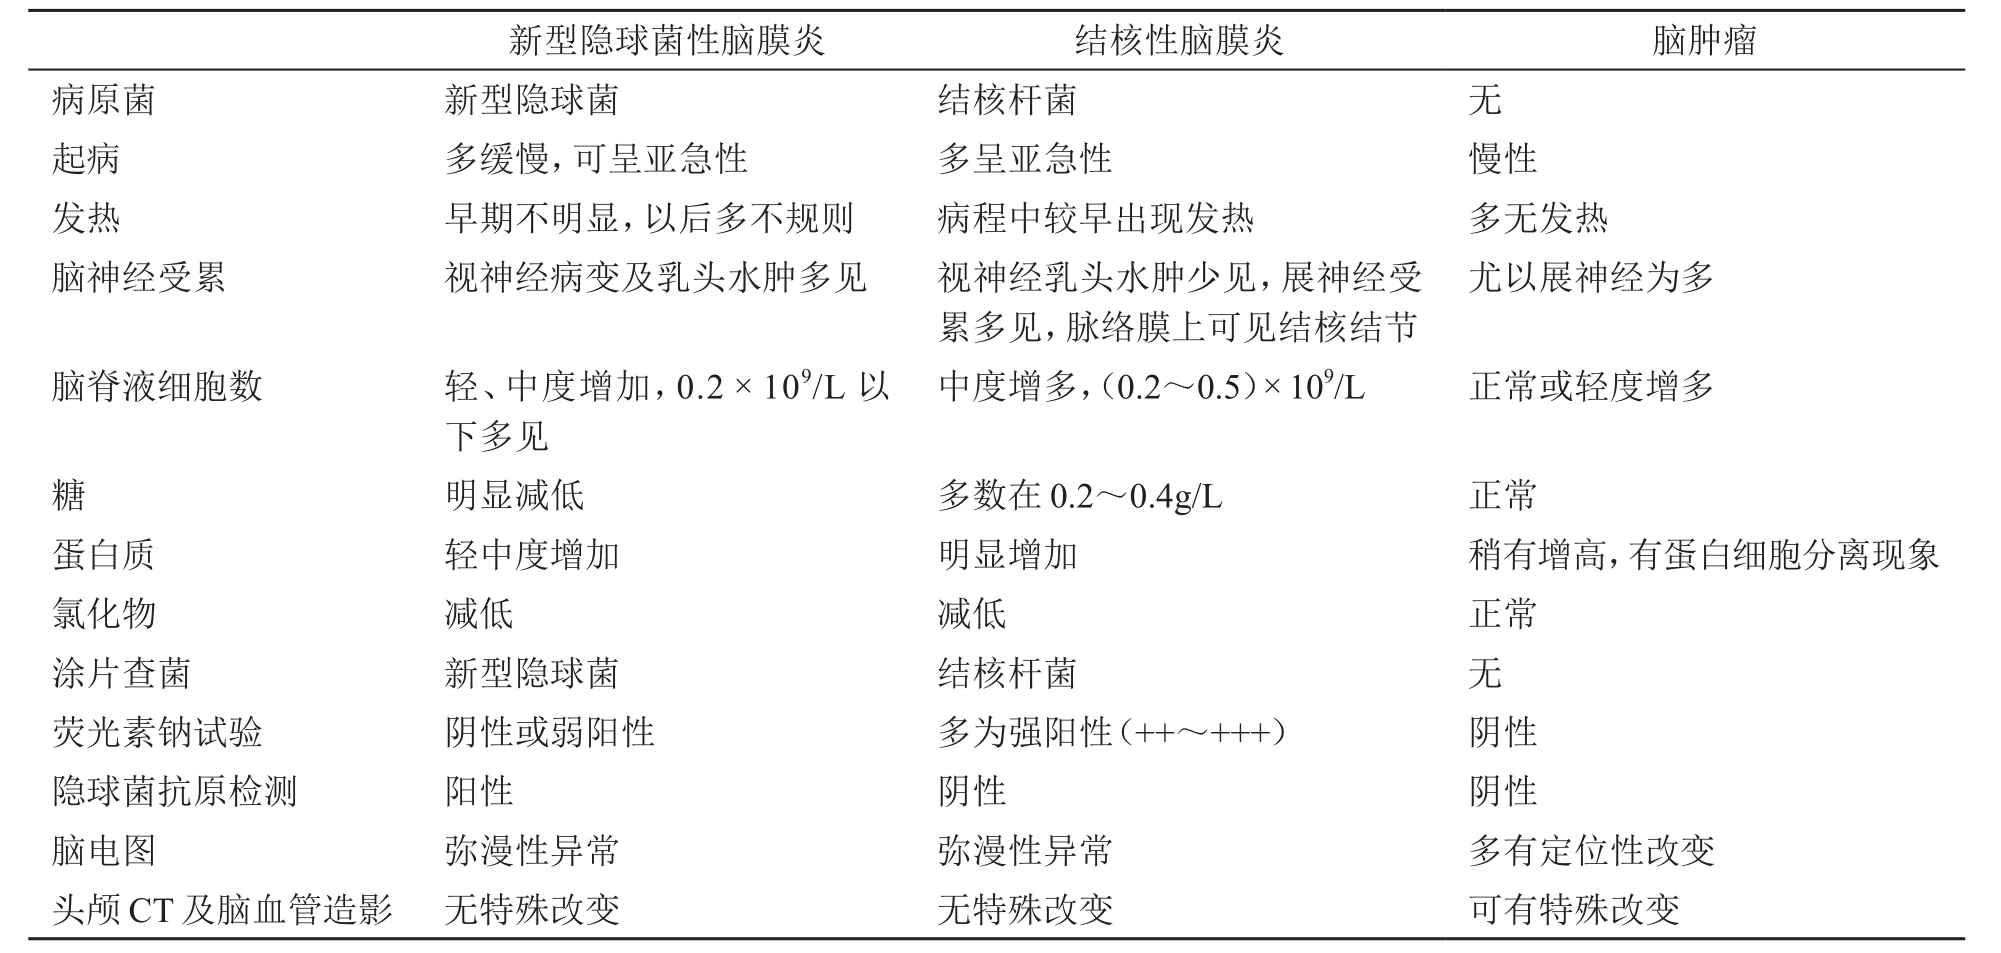
\includegraphics[width=6.66667in,height=3.16667in]{./images/Image00390.jpg}
\end{table}

卧床休息,加强护理。提供营养丰富易消化的饮食,保持水电解质平衡,防治并发症。脱水降颅压。酌情输血或血浆。尽可能停用抗生素、皮质激素及其他免疫抑制剂。适当使用改善脑营养代谢的药物,但维生素B\textsubscript{1}
、B\textsubscript{6} 、B\textsubscript{12}
、谷氨酸、麦芽糖、味精等,会助长隐球菌繁殖,应忌用。对伴严重颅内高压症或脑积水者,可酌情选用侧脑室穿刺引流或脑脊液分流术。

隐球菌性脑膜炎未经特效治疗者基本全部死亡,经药物治疗者即时有效率为60\%~70\%。20\%~30\%的初步获愈者有复发。少数治愈患者有严重后遗症,包括视力丧失、脑神经瘫痪、严重运动障碍、脑积水、智能障碍等。有下列情况预后不良:①有脑积水者;②诱发因素尚未消除者,如患者有淋巴瘤或应用激素;③CSF检查轻度异常或正常,涂片或培养阳性者;④血培养阳性;⑤治疗前血或CSF抗原滴定高或治疗后抗原滴度持续高、抗体缺少者。

\protect\hypertarget{text00250.html}{}{}

\section{病毒性脑膜炎}

病毒性脑膜炎(viral
meningitis)是一组由各种病毒感染引起的脑膜急性炎症性疾病,临床以发热、头痛和脑膜刺激征为主要表现。是临床上最常见的无菌性脑膜炎(aseptic
meningitis)。为一种良性自限性疾病,多无并发症。

\subsection{病因与发病机制}

病因有:①主要为肠道病毒(柯萨奇病毒、埃可病毒与脊髓灰质炎病毒),约占85\%~95\%。②其次为腮腺炎病毒、单纯疱疹病毒、腺病毒(主要是1、2、3、5、7型)、淋巴细胞脉络丛脑膜炎病毒、单核细胞增多症和带状疱疹病毒等。由肠道病毒引起的病毒性脑膜炎,发病高峰主要在夏季和早秋;腮腺炎病毒脑膜炎一般多见于冬、春季节,与腮腺炎同时流行;淋巴细胞脉络丛脑膜炎则以冬季较常见;而单纯疱疹脑膜炎无明显季节性。肠道病毒主要经粪-口途径,少数通过呼吸道分泌物传播,大部分病毒在下消化道发生最初感染,肠黏膜细胞有与肠道病毒结合的特殊受体,病毒经肠道入血后产生病毒血症,再经血液进入中枢神经系统。大多数病毒侵入机体后经病毒血症后侵犯脑膜,常同时存在不同程度地侵犯脑实质,但亦可单独累及脑膜。病理上呈现软脑膜弥漫性淋巴细胞浸润,脑组织有围管性淋巴细胞浸润,胶质增生、神经节细胞肿胀及点状出血。脉络膜丛及脑室上皮亦有非特异性炎症改变。

\subsection{诊断}

\subsubsection{临床表现特点}

本病具有以下临床特点:①发病年龄以10~40岁多见,约半数在15岁以下发病。②急性或亚急性起病(一般潜伏期约1周),常先有类似感冒或相应病毒所致全身症状,如畏寒、发热、头痛、咽痛与躯体不适、疼痛、腹泻、皮疹、乏力等。常有感觉过敏、感觉异常、畏光、肌痛与腹痛。症状的严重程度随患者的年龄增长而加重。③脑膜刺激症状:在全身症状同时或稍后短时间内出现,呈头痛、恶心,呕吐,颈软至中度抵抗,Kernig征和Brudzinski征阳性。体温很少超过40℃。可伴有意识障碍,如淡漠、嗜睡、谵语,甚至昏迷等;较少伴发脑炎症状如脑神经障碍、偏瘫与感觉障碍等。④某些特定病毒感染的征象:如腮腺炎的腮腺肿大和睾丸炎;某些肠道病毒感染可出现皮疹,大多与发热同时出现,持续4~10天,柯萨奇病毒A\textsubscript{5}
、A\textsubscript{9} 、A\textsubscript{16}
和埃可病毒(ECHO)\textsubscript{4} 、ECHO\textsubscript{6}
、ECHO\textsubscript{9} 、ECHO\textsubscript{15}
、ECHO\textsubscript{30}
感染,皮肤损害典型的为斑丘疹,皮疹可局限于面部、躯干或涉及四肢,包括手掌和足底部;柯萨奇病毒B组感染可有流行性肌痛(胸壁痛)和心肌炎;传染性单核细胞增多症病毒感染有全身淋巴结肿大压痛、伴剧烈咽痛或见黄疸等。

\subsubsection{辅助检查}

辅助检查的特点有:①周围血象白细胞数正常或中度增高,血沉增快;②脑脊液压力正常或轻度升高,无色透明,轻度或中度淋巴细胞升高(最初数小时内可以中性粒细胞为主),通常在(45~1500)×
10\textsuperscript{6}
/L以下。糖与氯化物正常或稍减,蛋白正常或中度增高(多在1.0g/L以内),或见有细胞蛋白分离现象。细菌和真菌涂片检查阴性。③急性期CSF与血液的病毒分离、恢复期的血清中和抗体滴定和补体结合反应检测可有阳性发现。

\subsubsection{诊断注意事项}

典型病例根据发热、头痛、恶心、呕吐、肌痛、脑膜刺激征,血液和CSF的改变等,诊断一般并不困难;但病原学的诊断常需依赖CSF中分离出病毒才可确诊。应注意与下述疾病鉴别:各种邻近脑膜的化脓性感染引起的脑膜反应,细菌性、结核性、真菌性脑膜炎,钩端螺旋体病脑膜炎,癌性脑膜病,单核细胞增多症等。

\subsection{治疗}

\paragraph{对症支持疗法}

卧床休息,富维生素饮食。头痛剧烈时可给予镇痛剂,高热用物理降温或给予退热剂。临床症状严重者,可短期内用小剂量地塞米松5~10mg/d加入液体静滴。

\paragraph{降颅内压}

有颅内压增高者,可用甘露醇、高渗葡萄糖液等行脱水疗法。

\paragraph{抗病毒治疗}

抗病毒治疗可明显缩短病程和缓解症状,目前针对肠道病毒感染临床上使用或试验性使用的药物有免疫血清球蛋白和抗微小RNA病毒药物普来可那立(pleconaril)。

本病绝大多数患者为自限性疾病,轻者3~5天完全恢复,重者可持续1~4周,平均于3周内痊愈,一般不留后遗症。

\protect\hypertarget{text00251.html}{}{}

\hypertarget{text00251.htmlux5cux23CHP8-3-5}{}
参 考 文 献

1. 张世荣
,张培元.结核性脑膜炎的诊断和治疗进展.中华结核和呼吸杂志,1996,19(2):69

2. 贾建平.神经病学.第6版.北京:人民卫生出版社,2008:238-244

3. 陈新谦,金有豫,汤光.新编药物学.第17版.北京:人民卫生出版社,2011

\protect\hypertarget{text00252.html}{}{}

\chapter{急性单纯疱疹病毒性脑炎}

急性单纯疱疹病毒性脑炎(acute herpes simplex virus
encephalitis,AHSE),系单纯疱疹病毒(herpes simplex
virus,HSV)感染引起的中枢神经系统(CNS)病毒感染性疾病,是CNS最常见的病毒感染性疾病,也是散发性致命性病毒性脑炎最常见的病因。本病呈全球分布,一年四季均可发病。在CNS中,HSV常累及大脑颞叶、额叶及边缘系统,引起脑组织出血性坏死和(或)变态反应性脑损害,又称为急性坏死性脑炎或出血性脑炎。

\subsection{病因与发病机制}

HSV是一种嗜神经DNA病毒,有两种血清型,即HSV-1
和HSV-2。患者和健康带毒者是主要传染源,主要通过密切接触与性接触传播,亦可通过飞沫传播。HSV首先在口腔和呼吸道或生殖器引起原发感染,机体迅速产生特异性免疫力而康复,但不能彻底消除病毒,病毒以潜伏状态长期存在体内而不引起临床症状。神经节中的神经细胞是病毒潜伏的主要场所,HSV-1主要潜伏在三叉神经节,HSV-2潜伏在骶神经节。原发感染通常发生于儿童期或少年期,感染后多不发生临床症状,或仅表现为胃炎或上呼吸道感染。当人体受到各种非特异性刺激使机体免疫力下降,潜伏的病毒再度活化,经三叉神经或其他神经轴突进入脑内,引起单纯疱疹病毒脑炎。成人超过2/3的HSV-1脑炎是由再活化感染而引起,也有少数单纯疱疹脑炎是作为HSV-1原发感染的一部分,病毒沿嗅神经入脑而致脑炎。而HSV-2则大多数由原发感染引起。在人类约90\%
的AHSE由HSV-1引起,仅10\%由HSV-2所致,且HSV-2所引起的AHSE主要发生在新生儿,是新生儿通过产道时被HSV-2感染所致。

本病脑部病理改变呈弥漫性,侵犯双侧大脑半球,但并不完全对称,常以颞叶、边缘系统及额叶受累最为严重,其他脑叶及脑干均可被累及。在致死病例,呈现严重的脑膜炎及脑实质广泛性破坏性改变,可见有坏死性、炎症性或出血性损害。受累神经细胞和胶质细胞核内可见嗜酸性包涵体(故称急性包涵体脑炎),是本病最有特征性的病理改变。在电子显微镜下可发现包涵体内含有病毒抗原及疱疹病毒颗粒。

\subsection{诊断}

\subsubsection{临床表现特点}

1.一般特征
本病散在发生而无季节性和地方性,可发生于任何年龄,约2/3的病例发生于40岁以上的成年人。原发感染的潜伏期为2~21天,平均6天。前驱期可有呼吸道感染,发热、乏力、头痛、呕吐等非特异性症状以及轻度行为、精神或性格改变。通常呈急性或亚急性起病,约1/4患者有口唇单纯疱疹病史。病后体温可高达38.4~40.0℃。病程为数日至1~2个月。

2.临床常见症状
包括头痛、呕吐、轻微的意识和人格改变、记忆丧失、轻偏瘫、偏盲、失语、共济失调、多动(震颤、舞蹈样动作、肌阵挛)、脑膜刺激征等。约1/3的患者出现癫痫发作。部分患者可因精神行为异常为首发或唯一症状而就诊于精神科,表现为注意力涣散、反应迟钝、言语减少、情感淡漠、表情呆滞、呆坐或卧床、行动懒散,甚至不能自理生活;或表现木僵、缄默;或有动作增多、行为奇特及冲动行为等。

3.病情常在数日内快速进展
,多数患者有意识障碍,表现意识模糊或谵妄,昏睡、昏迷,或去皮质状态。部分患者在发病早期迅即出现昏迷。重症患者可因广泛脑实质坏死和脑水肿引起颅内压增高,甚至脑疝形成而死亡。

\subsubsection{辅助检查}

\paragraph{脑脊液(CSF)检查}

脑脊液压力正常或轻度增高,重症者可明显增高;细胞数多增加,一般在(50~100)×
10\textsuperscript{6} /L,最多者可达1000 × 10\textsuperscript{6}
/L,淋巴细胞占优势,偶见中性为主。部分病例早期脑脊液中可出现大量红细胞,红细胞数达(50~500)×
10\textsuperscript{6}
/L或更多,脑脊液黄变,是本病有脑实质出血、坏死的反映。蛋白质轻~中度增加,糖和氯化物大多正常。约5\%~10\%病例初期脑脊液检查可完全正常。

\paragraph{脑电图(ECG)检查}

其典型改变示α节律丧失,弥漫性慢波,在额、颞叶出现高波幅周期性棘波和慢波。

\paragraph{CT或MRI检查}

90\%患者于病后数日CT扫描可见单侧或双侧颞叶、海马及边缘系统局灶性低密度区,扩展至额叶或顶叶,伴占位效应或强化,部分病例示出血性变化。有些病例早期CT正常,但MRI可显示灶性异常改变。

\paragraph{病毒学检查}

是确诊本病的依据。①双份CSF单纯疱疹病毒抗体(IgM、IgG)滴度增加4倍以上;单份CSF上述抗体>
1∶80;②血清中和抗体或补体结合抗体滴度逐渐增加到4倍以上或单份血清/脑脊液抗体滴度≤40;③检测CSF中HSV-DNA:用PCR检测病毒DNA,可早期快速诊断。

\paragraph{脑活检}

是诊断AHSE的金标准。细胞核内出现嗜酸性包涵体,电镜下可发现细胞内病毒颗粒。

\subsubsection{诊断注意事项}

本病临床诊断依据是:①口唇或生殖道疱疹史,或本次发病有皮肤、黏膜疱疹;②起病急,病情重,有发热、咳嗽等上呼吸道感染的前驱症状;③明显精神行为异常、癫痫发作、意识障碍和早期局灶性神经系统损害体征;④CSF细胞数增多或出现红细胞,糖和氯化物正常;⑤EEG示弥漫性异常,以颞、额区为主;⑥CT或MRI发现颞叶局灶性出血性脑软化灶;⑦特异性抗病毒药物治疗有效间接支持诊断。

确诊尚需选择如下检查:①双份血清和CSF检查发现HSV特异性抗体有显著改变趋势;②脑组织活检或病理发现组织细胞核内出现嗜酸性包涵体,或原位杂交发现HSV病毒核酸;③CSF-PCR检测发现病毒DNA;④脑组织或CSF标本HSV分离、培养和鉴定呈阳性。

临床上应注意与以下疾病鉴别:①带状疱疹病毒性脑炎:带状疱疹病毒可以长期潜伏在脊神经后根以及脑和脊髓的感觉神经节,当机体免疫力下降时,病毒被激活、复制、增殖,沿感觉神经传到相应皮肤引起皮疹,另一方面沿神经上行传播,进入CNS引起脑炎或脑膜炎。本病多见于中老年人,发生脑部症状与发疹时间不尽相同,多数在疱疹后数天或数周,也可在发疹之前,或无任何疱疹病史。临床表现为发热、头痛、呕吐、意识模糊、共济失调、精神异常及局灶性神经功能缺失征。病变程度相对较轻,预后良好。患者多有胸腰部带状疱疹的病史,头颅CT无出血性坏死的表现,血清及CSF检出该病毒抗体和病毒核酸阳性,可资鉴别。②肠道病毒性脑炎:该类病毒除引起病毒性脑膜炎外,也是病毒性脑炎的常见原因之一。多见于夏秋季,呈流行性或散发性发病。表现为发热、意识障碍、平衡失调、癫痫发作、肢体瘫痪等。一般恢复较快,在发病2~3周后症状即自然缓解。病程初期的胃肠道症状、CSF
中PCR检出该病毒核酸阳性可资鉴别。③其他疾病:还应与巨细胞病毒性脑炎、急性播散性脑脊髓炎、化脓性脑膜炎、脑脓肿、颅内占位性病变等相鉴别。

\subsection{治疗}

早期诊断和治疗是降低本病死亡率的关键。治疗主要包括抗病毒治疗,辅以免疫治疗和对症支持治疗。

\subsubsection{对症支持疗法}

患者常有较重的意识障碍和精神异常,必须加强护理,注意营养和水电解质平衡,及时吸痰,保持呼吸道通畅,防治肺炎和压疮,保持二便通畅。高热者降温,癫痫发作者行抗癫痫治疗等。必要时可给予复方氨基酸、脂肪乳等以增强机体抵抗力。

\subsubsection{抗脑水肿、降低颅内压}

通常选用甘露醇、高渗葡萄糖液、甘油果糖、呋塞米等作为脱水剂,其作用机制、应用方法及注意事项参见第41章“颅高压危象”。也可考虑用肾上腺皮质激素(见下述)。经上述药物治疗后,颅内压增高仍日益增重,甚至出现脑疝,应行紧急的脑室穿刺引流术和去骨瓣减压术。

\subsubsection{抗病毒治疗}

病毒侵入脑组织后,通常随着病程的进展,病毒量逐渐减少甚至消失,故必须早期使用抗病毒药物才有效果。常用的有:

\paragraph{阿昔洛韦(无环鸟苷,acyclovir,ACV)}

为广谱核苷类抗病毒药,能抑制病毒DNA的合成。阿昔洛韦首先在感染病毒的细胞内,经病毒胸苷激酶作用转化为单磷酸阿昔洛韦,再经宿主细胞中激酶作用转化为三磷酸阿昔洛韦,与DNA合成的底物2'{-}脱氧尿苷发生竞争,阻断病毒DNA链的合成。是治疗AHSE的首选抗病毒药物之一。当临床疑诊又无条件作CSF病毒学检查时可用阿昔洛韦进行诊断性治疗。口服吸收差,生物利用度仅15\%~30\%,血浆蛋白结合率为9\%~33\%,50\%可通过血脑屏障。血浆半衰期约2.5小时,肾功能不全时可延长至20小时,故肾功能不全者应减少剂量并充分饮水;同时不得并用其他肾毒性药物如氨基糖苷类抗生素、两性霉素B和环孢素等。用法:静脉滴注:15~30mg/(kg•d),分3次静脉滴注,连用14~21天。若病情重可延长治疗时间或再重复治疗一个疗程。使用前先将本品用注射用水配成2\%溶液,然后将每次剂量用生理盐水或5\%葡萄糖液加至100ml,于l小时内静滴完。口服每次200~400mg,每日4~5次,10天为l疗程。近年已发现对ACV耐药的HSV株,这类患者可试用膦甲酸钠和西多福韦治疗。

\paragraph{更昔洛韦(ganciclovir)}

本品进入细胞后由病毒的激酶诱导生成三磷酸化物,竞争性抑制病毒的DNA聚合酶而终止病毒DNA链增长。抗HSV的作用是ACV的25~100倍,具有更强、更广谱的抗HSV作用和更低的毒性。对ACV耐药的HSV株本品亦敏感。用量是5~10mg/(kg•d)静脉滴注,每12小时1次,疗程14~21天。主要副作用是肾功能损害和骨髓抑制(中性粒细胞、血小板减少),与剂量相关,停药后可以恢复。

\paragraph{阿糖腺苷(adenine arabinoside,Ara-A)}

为较广谱的DNA病毒抑制剂,动物实验显示强大抗病毒效应。能很好通过血脑屏障,其脱氧后的第一个代谢产物阿糖次黄嘌呤(Aar-HX)也有抗病毒效果,故有较持久的治疗作用。副作用轻且少,可有疼痛综合征(包括全身痛、肌肉痛、关节痛、神经痛等)、胃肠道反应(恶心、呕吐、腹泻、纳差等),偶见可逆性骨髓抑制。停药后均可自行消失。对肝肾损害较轻。孕妇禁用,哺乳期妇女、婴幼儿、肝肾功能不全和造血功能不良者忌用。用法:通常成人剂量10~20mg/(kg•d),连用7~10天。由于溶解度低,每毫升浓度不超过0.7mg,半衰期短(仅1.5小时),故每日须缓慢静滴12小时以上。必要时间隔l周后再用1疗程。

\paragraph{利巴韦林(ribavirin,病毒唑,virazole)}

为广谱抗病毒药。对某些类型的疱疹病毒、痘病毒、流感病毒、副流感病毒、鼻病毒、呼吸道合胞病毒、肠病毒等DNA和RNA病毒均有效。作用机制可能是抑制了磷酸次嘌呤核苷脱氢酶,使鸟嘌呤核苷酸不能合成,阻止病毒核酸的合成,从而抑制病毒复制。口服易吸收、血浆半衰期约72小时。不良反应少,少数患者服药后产生腹泻、白细胞减少、贫血等,停药后可恢复正常。妊娠妇女禁用。用法:口服每次300mg,每日3~4次;静脉滴注或肌内注射,每日为10~15mg/kg,分2次用,静滴宜缓慢。

\subsubsection{免疫治疗}

\paragraph{干扰素(interferon)及其诱导剂}

具有广谱抗病毒作用,对RNA病毒的作用比对DNA病毒更为敏感。干扰素进入细胞后可与宿主细胞抗病毒蛋白的密码抑制物相结合后除去抑制,产生的抗病毒蛋白可抑制各种病毒的酶、核酸和蛋白质的合成,从而阻断病毒的复制与繁殖。它除了有直接的抗病毒作用以外,还有重要的免疫调节作用,可增强HLA抗原在病毒感染细胞膜上的表达,激活抗原递呈细胞,加强特异性细胞毒性T淋巴细胞的应答,加强自然杀伤细胞的活性,也可调节细胞因子,如白细胞介素l、2和肿瘤坏死因子的产生。干扰素且可直接作用于B细胞,对免疫球蛋白的产生呈量效关系。用法:α-干扰素每次60
× 10\textsuperscript{6}
U,每日1次深部肌内注射,连续30天;亦可用β-干扰素全身用药与鞘内注射联合治疗。应用干扰素诱导剂可使机体细胞产生内源性干扰素。目前临床上使用的干扰素诱导剂是聚肌苷酸-聚胞苷酸(polyriboinsinepolyribocyaidylic
acid,Polyl:C),简称聚肌胞。它可增加干扰素水平,抑制病毒复制和向中枢神经系统蔓延。用法:2ml/次,肌肉注射,每日2次。临床上可与其他抗病毒药物联合应用。

\paragraph{转移因子}

可使正常淋巴细胞致敏而转化为免疫淋巴细胞,治疗剂量为皮下注射每次1支,每周1~2次。

\paragraph{肾上腺皮质激素}

有争议,但肾上腺皮质激素能控制AHSE炎症反应和减轻水肿,对病情危重、头颅CT见出血性坏死灶以及CSF白细胞与红细胞明显增多者可酌情使用。地塞米松10~20mg/d加入液体静滴,连用10~14天;或用甲泼尼龙大剂量冲击疗法,0.5~1.0g/d,连用3~5天,随后改用泼尼松口服(60mg/d),以后逐渐减量。

\subsubsection{抗菌治疗}

合并细菌或真菌感染时应根据药敏结果选用适当的抗生素或抗真菌治疗。

\subsubsection{脑细胞代谢活化剂的应用}

可选用ATP、CoA、细胞色素C、胞磷胆碱、脑活素等,以改善脑细胞的代谢,促进脑功能的恢复。参见第25章“急性脑功能衰竭”治疗部分。

本病预后取决于病情和治疗是否及时。若未经抗病毒治疗、治疗不及时或不充分,病情严重则预后不良,病死率可高达60\%~80\%。若及早给予了足量的抗病毒药物治疗或病情较轻,多数患者可治愈。但约10\%患者可遗留不同程度的瘫痪、智力下降等后遗症。

\protect\hypertarget{text00253.html}{}{}

\hypertarget{text00253.htmlux5cux23CHP8-4-4}{}
参 考 文 献

1. 贾建平.神经病学.第6版.北京:人民卫生出版社,2008:233-236

2. 陈新谦,金有豫,汤光.新编药物学.第17版.北京:人民卫生出版社,2011

\protect\hypertarget{text00254.html}{}{}

\chapter{脑 囊 虫 病}

脑囊虫病(cerebral
cysticercosis)是指猪带绦虫的幼虫(囊虫或称囊尾蚴)寄生于中枢神经系统形成包囊,导致以神经精神障碍为主要临床表现的疾病。在我国分布广泛,各地均有散发,但以东北、西北、华北、河南及内蒙古较多,长江以南地区发病率较低。是我国北方症状性癫痫常见的病因之一。人群普遍易感,但以21~40岁青壮年多见,男多于女,农村高于城市。

\subsection{病因与发病机制}

本病主要是由于食用未经恰当处理的含绦虫卵的食物、饮水所致。猪绦虫病患者是本病的唯一传染源。患者粪便中排出的虫卵对自体及周围人群均有传染性。其感染方式为:①自身感染:包括两种,内源性自身感染指猪绦虫病患者由于呕吐或肠道逆蠕动,使绦虫妊娠节片反流入胃,虫卵在胃、十二指肠被消化液作用,六钩蚴逸出而致感染;外来性自身感染指猪绦虫病患者的手指污染自己粪中的绦虫卵,再食入胃中而感染。②外源性感染(异体感染):患者自身并无猪绦虫病,因摄入染有他人粪便中猪绦虫卵的食物、蔬菜、瓜果而感染。外源性感染的发生率较自身感染为高。进入胃内的猪绦虫虫卵(内含六钩蚴),在十二指肠被消化液作用,六钩蚴破膜而出钻入肠壁,随后进入肠系膜小静脉及淋巴循环而被输送至全身各组织器官,虫体逐渐长大,演变为囊尾蚴,寄生于皮下、肌肉、脑组织等处。六钩蚴可通过血液循环进入脑实质,大多寄生于大脑皮质邻近运动中枢,囊虫的大小、数目很不一致,一般由米粒至豌豆大小,50\%的患者仅1~2个囊虫,但有时达数百个甚至数千个之多,大多分散各处。囊虫侵入脑实质或脑膜以后引起局部反应性炎症变化,在囊虫的四周,如同异物的四周一样,形成纤维结节组织性被膜。六钩蚴亦可经血液循环于脉络膜丛进入脑室系统及蛛网膜下腔。寄生脑室内囊虫常为单个,游离或带蒂系于脑室壁,引起局部室管膜炎,产生室管膜肥厚和瘢痕性条索,致使脑室变形,脑脊液循环障碍;同时由于脉络丛受到囊虫毒素的影响,脑脊液的分泌增多,发生严重的颅内压增高和脑内积水;又因囊虫的飘动阻塞脑脊液循环而加重颅内压增高。囊尾蚴位于小脑延髓池、小脑脑桥角等部位时常伴有继发性增生性蛛网膜炎。囊虫寄生的局部产生轻度炎症,在脑膜者有脑膜增厚、粘连,类似结核性脑膜炎;粘连重者,脑脊液循环、吸收障碍,产生交通性脑积水。弥漫性脑囊虫病患者脑内含有大量囊尾蚴,可产生广泛脑组织破坏与炎症病变。周围脑组织在急性期有水肿、坏死,镜下有炎症细胞浸润;慢性期有萎缩、异物反应和机化。囊虫的寿命可活到数年至数十年不等,少数长达20年或以上,虫体死后发生纤维化和钙化,此时对机体并非无害,它使慢性炎症继续下去,同时又成为对周围组织发生经常性机械刺激和化学刺激的根源,比起活囊虫来,甚至可引起更加严重的变化。

\subsection{诊断}

\subsubsection{病史}

有食“米猪肉”史,或有肠绦虫病史,或粪便中发现绦虫卵或妊娠节片,且有皮下或肌肉结节等全身囊虫病体征病史,均有助于诊断。

\subsubsection{临床表现特点}

本病的临床表现极为复杂多样,从全无症状到引起猝死不等,症状因囊虫所在部位、数量及生物学状态不同(发育、静止或死亡期)而不同。通常病程缓慢,自感染到出现症状,数日至30年不等,多在5年以内。按囊虫在CNS中的位置不同,其临床症状可分为以下几型:

\paragraph{脑实质型}

占80\%以上。囊尾蚴常位于大脑皮质表面邻近运动中枢区,临床表现以癫痫最为常见,以反复发作的各种类型癫痫为特征。约半数患者表现为单纯大发作,此外尚有失神、发作性幻视、视物变形、精神运动性兴奋及各种局限性抽搐和感觉异常。同一患者可表现为几种发作形式,且易于转换。这种发作形式的多样性及易转换性为本病特征之一。发作后有一过性肢体瘫痪、脑神经麻痹或失语、失明。大发作发生频率较低,可数月至数年1次。约1/10患者的癫痫发作可有自行缓解倾向。弥漫性脑实质受累者常引起颅内压增高或器质性精神病,甚或因脑组织破坏和皮质萎缩导致痴呆。罕见的情况是在感染初期发生急性弥漫性脑炎,引起意识障碍甚至昏迷。

\paragraph{蛛网膜型}

占脑囊虫病的10\%,常与其他各型合并发生。以不伴明显脑实质病损的脑膜损害为主。脑膜的包囊破裂或死亡可引起脑膜刺激症状、交通性脑积水和脑膜炎等表现;CSF可呈炎症改变,压力增高,细胞数约(10~100)×
10\textsuperscript{6}
/L,以淋巴细胞为主;蛋白增高,糖定量大多正常,个别患者可低于2.2mmol/L(40mg/dl),每易误诊为结核性脑膜炎或病毒性脑膜炎。包囊在基底池内转化为葡萄状后不断扩大,引起阻塞性脑积水;脊髓蛛网膜受累出现蛛网膜炎和蛛网膜下腔完全阻塞;均表现为颅内压增高的症状与体征。

\paragraph{脑室型}

占脑囊虫病的10\%。四脑室较多见,侧脑室、室间孔、三脑室、导水管依次明显减少。在第三和第四脑室内的包囊可阻塞脑脊液循环,导致阻塞性脑积水,引起颅内压增高。包囊可在脑室腔内移动,并产生一种球状活瓣作用,可突然阻塞第四脑室正中孔,造成急性脑脊液循环障碍,导致脑压突然急骤增高,引起剧烈头痛、呕吐、眩晕、意识障碍和跌倒,或循环呼吸障碍而猝死,或发生小脑扁桃体疝,常因体位改变而诱发,谓之布龙征(Brun
sign),或体位改变综合征。该类患者常有颈项强直,强迫头位。少数患者可在没有任何前驱症状的情况下突然死亡。

\paragraph{脊髓型}

由于囊虫侵入椎管压迫脊髓,产生脊髓受压征。临床表现为截瘫、感觉障碍、大小便潴留等。此型罕见。

\paragraph{混合型}

兼有上述两型或以上表现。以脑实质型与脑室型混合为多见,会使症状更为复杂,亦有表现为幻觉、迫害妄想等精神症状者。

脑囊虫病各型间可相互交叉或转化。绝大多数患者同时存在皮下结节(约90\%),结节可在脑部症状发生前或后出现,个别患者在皮下结节出现后22年始出现癫痫发作。皮下结节数目自数个至数百、数千个不等,以头部、躯干较多,四肢较少。皮下结节可自由移动,与皮肤组织不粘连,不痛不痒,也无炎症反应及色素沉着。结节可分批出现,亦可逐渐自动消失。结节大小约0.5~1.0cm。

\subsubsection{辅助检查}

\paragraph{粪便检查}

有绦虫病者大便中可发现绦虫节片,亦可查出绦虫卵。

\paragraph{血液嗜酸性粒细胞计数}

本病40\%~50\%患者增多。

\paragraph{免疫学检查}

可采用患者的血液或脑脊液作囊虫间接血凝试验(IHA)、酶联免疫吸附试验(ELISA)等。IHA操作简便,灵敏度和特异性高。凡受检血清稀释1∶50以上呈较强沉淀反应者可确定为阳性。ELISA的特异性和灵敏性与IHA相同,其阳性血清的平均效价较后者为高。

\paragraph{脑脊液}

除可作免疫学检查外,50\%患者腰穿压力> 200mmH\textsubscript{2}
O,约60\%白细胞在10 × 10\textsuperscript{6} /L以上,个别有糖减少。

\paragraph{X线平片}

肌肉内钙化影较常见,阳性率达70\%左右;颅内囊虫钙化影阳性率较低,一般5.54\%~10\%左右。

\paragraph{头颅 CT检查}

能显示囊虫的位置、数量、大小、是否钙化以及脑水肿、脑积水和脑室形态。脑囊虫在CT所见主要为集中或散在的直径0.5~1.0cm的圆形、椭圆形或不规则形阴影,可呈低密度、高密度或高低混杂密度影;增强扫描头节可强化。

\paragraph{MRI检查}

囊虫病灶常比CT更清晰,有时CT阴性,MRI则能发现囊虫的信号影。

\paragraph{脑室造影}

当有脑室扩大、疑有脑室内囊虫而CT未发现时可作脑室造影。

\paragraph{脑血管造影}

当疑有脉管炎引起的脑梗死时可作DSA,一般不作此检查。

\paragraph{活组织检查}

皮下结节应常规做活组织检查,病理切片中见到囊腔中含有囊尾蚴头节为特征。

\subsubsection{诊断注意事项}

皮下结节和眼囊虫病(可发生于眼的任何部位,但以发生在玻璃体最为常见,几近半数,其次为视网膜)临床较易诊断;脑囊虫病如不伴有皮下结节则诊断较为困难。在我国东北、西北、华北等地区的农村,凡具有癫痫发作、颅内压增高、精神障碍等三大症状者应首先考虑脑囊虫病的可能,若有皮下结节并存,当为有力的佐证。免疫学检查、皮下结节的囊虫活检和头颅CT、MRI检查均有助于诊断。

孤立的脑囊虫需与巨大单发的蛛网膜囊肿或脑脓肿鉴别;多发囊泡型脑囊虫需与多发性脑转移瘤、多发性腔隙性脑梗死鉴别。脑囊虫病引起的癫痫须与原发性癫痫以及血吸虫病、肺吸虫病等所致的癫痫相鉴别;蛛网膜型的脑囊虫病需与结核性或隐球菌性脑膜炎相鉴别,详见有关章节。

\subsection{治疗}

\subsubsection{药物治疗}

\paragraph{阿苯达唑(丙硫咪唑,albendazole)}

是一种广谱、高效、安全的抗蠕虫药,为治疗囊虫病的首选药物,对脑型和皮肤肌肉型囊虫病均具良效,显效率达85\%,治愈率为50\%左右。口服后胃肠道吸收良好,并能通过血脑屏障对脑内囊尾蚴起作用。从小剂量开始,每日15~20mg/kg,分2~3次服用,成人总剂量为300mg/kg。间隔3~4周可重复第2个疗程,一般可连用3~4个疗程。有颅内压增高者,可先用甘露醇及地塞米松静滴,待颅压下降再开始治疗。治疗半年后进行复查,需要时再重复治疗。本药毒性较强,主要是囊虫被杀死后异性蛋白的毒性反应或变态反应。严重肝、肾、心功能不全者慎用,孕妇及哺乳期禁用。

\paragraph{吡喹酮(praziquantel)}

是一种广谱抗蠕虫药,作用快、疗效高,口服经肠道吸收,在肝脏破坏,其代谢产物从尿中排泄,可直接杀死囊尾蚴,通过破坏头节结构使其失去生活能力而死亡。对皮肤肌肉型的囊虫病具有很高的疗效,对脑囊虫病亦有较好的疗效。从小剂量开始,200mg/d,分2次口服,然后根据用药反应逐渐加量,但不超过1000mg/d,成人总剂量为300mg/kg。囊虫数量少、病情较轻者,加量可较快;囊虫数量多、病情较重者,加量宜缓慢。2~3个月后开始第二疗程,共3~4个疗程。亦有间隔1个月开始一疗程的。症状重者剂量可小些,一个疗程的时间可长些。患者必须住院治疗,因在治疗过程中,因囊虫被杀死后的毒性作用,可引起脑组织的炎性反应及水肿,副作用一般在用药后第2天至用药后两周之间出现。可出现头痛、发热、皮疹等反应,少数患者可出现休克、癫痫发作加重、颅内压增高等现象,重者可导致死亡。一般无需终止治疗,治疗中宜辅用脱水剂、皮质激素与抗惊厥药物等。吡喹酮可制成栓剂治疗囊虫病;还有注射剂,每日l次肌注500mg,5~7天为1疗程。有精神障碍与痴呆表现的脑囊虫病者,本品治疗易诱发精神异常,不宜采用。有眼囊虫病者服用本品后局部炎症反应较剧,增加手术的复杂性,应列为禁忌。

\subsubsection{手术治疗}

脑室系统单个囊虫阻塞脑脊液循环者,应手术摘除,疗效较好。对颅内压显著增高而药物治疗无效者,亦可考虑手术减压。眼内囊虫病不宜用杀虫药物治疗,因为囊虫死亡后引起炎症反应可加重视力障碍,故以手术摘除为主。有脑积水者可行CSF分流术以缓解症状。

\protect\hypertarget{text00255.html}{}{}

\hypertarget{text00255.htmlux5cux23CHP8-5-4}{}
参 考 文 献

1. 史玉泉.实用神经病学.第2版.上海:上海科学技术出版社,1994:447

2. 丁罗兰
,刘沛泽.脑囊虫病诊治中的几个问题.中国实用内科杂志,1994,14(4):222

3. 贾建平.神经病学.第6版.北京:人民卫生出版社,2008:251

4. 彭文伟.传染病学.第6版.北京:人民卫生出版社,2004:273

\protect\hypertarget{text00256.html}{}{}

\chapter{急性播散性脑脊髓炎}

急性播散性脑脊髓炎(acute disseminated
encephalomyelitis,ADEM),也称急性血管周围髓鞘脱失(acute perivascular
myelinoclasis),或播散性血管髓鞘病(disseminated
vasculomyclinopathy),是广泛累及脑和脊髓白质的急性炎症性脱髓鞘疾病,通常发生在感染后、出疹后或疫苗接种后。其病理特征为多灶性、弥散性髓鞘脱失。临床上主要表现为急起发热、头痛、呕吐、抽搐、脑膜刺激征、脑局灶体征、精神症状及意识障碍,甚至可出现昏迷及脊髓损害症状。

\subsection{病因与发病机制}

本病发生在狂犬病、乙脑、牛痘、风疹、百日咳、白喉、伤寒、脊髓前角灰白质炎等疫苗接种后者称为接种后脑脊髓炎(postvaccinal
encephalomyelitis,PVE);发生在多种感染性疾病和麻疹、风疹、天花、水痘、带状疱疹、流行性感冒、猩红热、百日咳、传染性单核细胞增多症或腮腺炎后者,称为感染性或感染后脑脊髓炎(postinfectious
encephalomyelitis,PIE);病前既没有接种史,也没有感染史的病例,称为特发性脑脊髓炎,一般就统称ADEM。本病的发病机制尚不明了,可能的机制是机体在病毒感染、疫苗接种或是服用某些药物后,这些致病因子侵犯了中枢神经系统,改变了其抗原性,或是由于某种因素引起了隐蔽抗原的释放,从而导致机体发生针对自身髓鞘的免疫攻击。

病理表现主要是静脉周围出现炎性脱髓鞘,病变散布于大脑、脑干、小脑和脊髓的灰质和白质,以白质为主。病灶多围绕在小和中等静脉周围。脱髓鞘区可见小神经胶质细胞,血管周围有炎性细胞浸润形成血管袖套。病势暴发、凶险,病理改变显示中枢神经系统白质坏死、出血明显者,称为急性坏死性出血性脑脊髓炎(acute
necrotizing hemorrhagic
encephalomyelitis,AHNEM),或急性出血性坏死性白质脑病(acute
hemorrhagic
leukoencephalopathy,AHNL),或急性出血性白质脑炎,为ADEM的暴发型。

\subsection{诊断}

\subsubsection{临床表现特点}

本病可发生在任何年龄,但以儿童与青壮年期发病为多,无季节性,多为散发,男女发病率差异不大。起病急,通常在感染后4~30天(以7~14天为多见),或疫苗接种后2~25天(以10~12天为多见)出现临床症状。常在发热缓解期,或疫苗接种反应高峰后几天,突然再度发热,并可有头昏、头痛、乏力、全身酸痛、背部僵硬等症状;若病情进展,则1~2天内很快出现程度不同的神经系统实质性症状,包括脑、脑干、小脑、脊髓、脑神经或(及)脊神经根、神经丛、单或多神经炎的表现。病情轻重,差别颇大。临床一般可分为脑型、脊髓型和脑脊髓型。脑型者突发头痛、呕吐、嗜睡和神志不清,并有脑膜刺激征;亦可有精神症状如幻觉、妄想等;如视神经受累,还可有视力减退或丧失,其他脑神经亦可受累;大脑半球或脑干病变分别导致偏瘫或四肢瘫;有些病例可并发癫痫发作。严重病例可出现昏迷及去大脑强直,少数可出现颅内压增高、视乳头水肿等。脊髓型突发弛缓性四肢或下肢瘫痪、感觉缺乏(通常在中胸段水平以下)及膀胱麻痹。脑脊髓型因损害广泛病情常较严重。流行性感冒后或狂犬病疫苗接种后脑脊髓炎(尤其是老年患者)尚可有周围神经受累、吉兰-巴雷综合征样的上升性麻痹。

ANHEM是ADEM暴发型。常见于青壮年,病前1~2周内可有上呼吸道感染史,起病急骤,病情凶险,症状体征在2~4天内达高峰,表现为高热、意识模糊或昏迷进行性加深、烦躁不安、痫性发作、偏瘫或四肢瘫。脑脊液压力增高,细胞数增多;脑电图弥漫慢活动。头颅CT见大脑、脑干和小脑白质不规则低密度区。死亡率高。

不同病因的ADEM的临床特点不同,见表\ref{tab89-1}。

\subsubsection{辅助检查}

\paragraph{脑脊液检查}

脑脊液压力正常或增高,细胞数轻~中度增多,以淋巴细胞为主;蛋白含量正常或轻度增加,糖和氯化物正常。ANHEM则以多核细胞为主,红细胞常见。

\paragraph{颅脑}

CT与MRI扫描
CT平扫可见脑白质内有大小不等的片状低密度影,增强后,可见病灶周边或内部不完整的带状或环状影及多灶结节影。MRI检查能更清晰地发现病变。

\paragraph{脑电图检查}

EEG常见弥漫的θ和δ波,亦可见棘波和棘慢复合波。

\subsubsection{诊断注意事项}

根据感染或疫苗接种后急性发病的脑实质弥漫性损害、脑膜受累和脊髓炎症状,脑脊液单核细胞数增多,EEG广泛中度异常,CT与MRI扫描显示脑和脊髓内多发散在病灶等可作出临床诊断。但应与以下疾病鉴别:①单纯疱疹病毒性脑炎:本病高热、抽搐常见,ADEM相对少见;脑脊液检查前者单纯疱疹病毒抗体滴度增高,且MRI表现大脑颞叶、额叶的异常信号,而ADEM则表现为弥漫性的异常信号,以白质损害为主。②多发性硬化(MS):MS一般无前期感染史,症状体征以局灶的神经功能损害为主,全脑症状损害不明显;ADEM意识障碍、精神症状等全脑症状明显。此外MS是多相病程,即反复发作的特点,而ADEM是单相病程。

\begin{table}[htbp]
\centering
\caption{急性播散性脑脊髓炎的类型及临床特点}
\label{tab89-1}
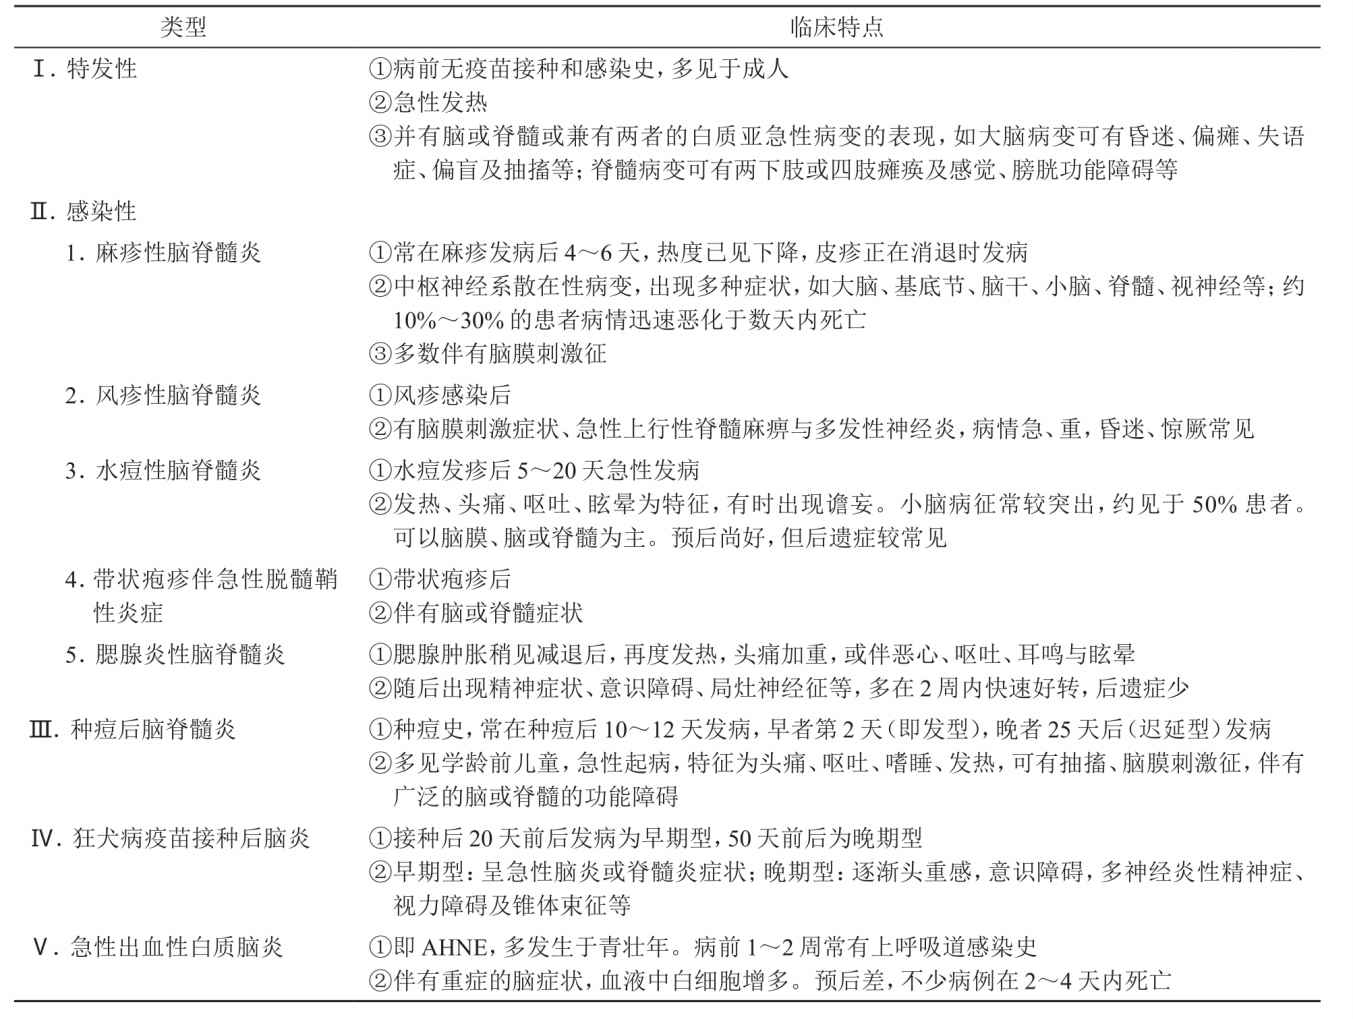
\includegraphics[width=6.67708in,height=5.03125in]{./images/Image00391.jpg}
\end{table}

\subsection{治疗}

\paragraph{肾上腺皮质激素}

肾上腺皮质激素早期、足量应用是治疗ADEM的主要措施,作用机制是抑制炎性脱髓鞘的过程,减轻脑和脊髓的充血水肿,保护血脑屏障。可用甲泼尼龙0.5~1.0g/d,或地塞米松20~30mg/d,或氢化可的松300~500mg/d加入液体中静滴冲击治疗,以后逐渐减为泼尼松口服。免疫球蛋白静脉滴注可取得较好效果。用法:成人0.4g/(kg•d)静脉滴注。连用3~5天为一疗程。

\paragraph{血液净化疗法}

对重型患者,有条件时可应用血浆置换疗法。

\paragraph{对症支持疗法}

包括加强护理,镇静止痉,脱水降颅内压,脑细胞代谢活化剂的应用,维持水电解质平衡,防治感染以及各种并发症等,参见有关章节。

本病因病情轻重及诱因不同,病死率约在5\%~30\%。幸存者多在2~3周后开始逐渐好转,绝大多数病例有相当大程度的恢复,不少患者得以痊愈。部分存活者常遗留明显的功能障碍,儿童恢复后常伴精神发育迟缓或癫痫发作等。

\protect\hypertarget{text00257.html}{}{}

\hypertarget{text00257.htmlux5cux23CHP8-6-4}{}
参 考 文 献

1. 张文武 .急诊内科学.第2版.北京:人民卫生出版社,2007:978

2. 专题笔谈.急性播散性脑脊髓炎的诊治.山东医药,1996,26(2):38

3. 贾建平.神经病学.第6版.北京:人民卫生出版社,2008:266

\protect\hypertarget{text00258.html}{}{}

\chapter{急性脊髓炎}

急性脊髓炎(acute
myelitis)系指各种感染后引起自身免疫反应所致的急性横贯性脊髓炎性病变,又称急性横贯性脊髓炎(acute
transverse
myelitis),是临床上最常见的一种脊髓炎。临床表现为病损平面以下的肢体瘫痪、传导束性感觉缺失和以膀胱、直肠功能障碍为主的自主神经功能损害。为神经科常见急症之一。一年四季均可发病,但以冬末春初或秋末冬初较为常见。

\subsection{病因与发病机制}

病因未明,包括不同的临床综合征,如感染后脊髓炎和疫苗接种后脊髓炎、脱髓鞘性脊髓炎(急性多发性硬化)、坏死性脊髓炎和副肿瘤性脊髓炎等。由于多数患者在脊髓症状出现之前1~4周有发热、上呼吸道感染、腹泻等病毒感染的症状,但其脑脊液未检出病毒抗体,脊髓和脑脊液中未分离出病毒,因此,目前多认为本病可能是病毒感染后所诱发的一种自身免疫性疾病,并非直接感染所致,为非感染性炎症性脊髓炎(myelitis
of noninfectious inflammatory
type)。外伤和过度疲劳可能为其诱因。病损可涉及脊髓多个节段,以胸髓(T\textsubscript{3~5}
)最多见,次为颈髓和腰髓。病变可能仅累及脊髓的灰质、白质,亦可累及脊膜、脊神经根和脑实质。多数病例以累及软脊膜、脊髓周边的白质为主,少数以累及中央灰质为主。病损可为局灶性、横贯性,多灶融合或散在于脊髓多个节段,但以前者为最多见。主要病理改变为脊髓充血、水肿和神经纤维的髓鞘脱失。轻症或早期患者,主要病变仅累及血管周围,出现血管周围的炎性细胞渗出和髓鞘脱失,表现为血管周围透亮区,严重者可融合成片状或呈空洞状;病情严重或晚期患者,常可见到溶解区的星形胶质细胞增生,并随病程延长而逐步形成纤维瘢痕,脊髓萎缩。脊髓膜常有原发或继发受累,表现为血管内皮细胞肿胀,血管周围炎性细胞渗出,早期为血管通透性增加,晚期则因缺血和血管内皮变性可致血管闭塞。

\subsection{诊断}

\subsubsection{临床表现特点}

本病任何年龄均可发病,但以儿童和青壮年多见,尤以农村青壮年为多。散在发病。典型病例在脊髓症状出现前1~2周常有上呼吸道感染、消化道感染症状或疫苗接种史等,外伤、疲劳、受凉等为发病诱因。但在神经症状出现时不伴发热。急性或亚急性起病,有的可先有背部疼痛、根痛、胸腹束带感等神经根刺激症状,随之急骤发生肢体麻木、无力,在数小时至数日内发展到脊髓完全性横贯损害。亦有患者无任何其他症状,而突然发生瘫痪。脊髓炎的临床表现,取决于受累脊髓的节段和病变的范围,脊髓各段均可受累,以胸段最为常见(74.5\%),其次为颈段(12.7\%)和腰段(11.7\%)。主要表现有:

\paragraph{运动障碍}

病变部位支配的肌肉呈现下运动神经元性瘫痪;病变部位以下支配的肢体呈现上运动神经元性瘫痪。病变早期呈现“脊髓休克”状态(其原因可能为脊髓低级中枢突然失去高级中枢的抑制控制,脊髓中枢的神经元又尚未有独立功能的一种暂时的功能紊乱现象),表现为弛缓性瘫痪,肢体肌张力降低,腱反射消失,病理反射阴性,腹壁、提睾反射均消失。若累及呼吸肌则表现为呼吸困难,咳嗽无力。一般持续2~4周则进入恢复期,肌张力逐渐增高,腱反射活跃,出现病理反射,肢体肌力的恢复常始于下肢远端,然后逐步上移。脊髓休克期长短取决于脊髓损害严重程度和有无发生肺部感染、尿路感染、压疮等并发症。70\%~80\%的脊髓炎,3个月恢复良好。但是,脊髓损害严重而又完全的患者,在休克期后,可以出现伸性反射、肌张力增高,但不伴肌力的恢复。这些患者脊髓本身的兴奋性逐步提高,下肢任何部位(足底、大腿内侧、小腿等)的刺激均可引起肢体屈曲反射或阵挛,这种反射的出现仅提示脊髓自主功能建立,并不意味脊髓病损的恢复。脊髓损害不完全者,常呈伸性肌张力增高,两腿内收,足内旋而呈剪刀交叉,刺激足底或大腿内侧可引起肢体抽动和阵挛。脊髓完全损害者,常呈屈性肌张力增高,严重者可为两腿屈曲如虾,此时若给轻刺激如膀胱充盈、足底、大腿内侧或腹壁受压,甚至棉被的压迫均可引起强烈的肢体屈曲痉挛、出汗、竖毛,重则出现血压升高和大、小便排出等症状,称为总本反射,一般预后较差。

\paragraph{感觉障碍}

病损平面以下深浅感觉均消失,有些患者在感觉消失区上缘可有1~2个节段的感觉过敏带、根痛或束带样疼痛感。局灶性脊髓炎者可能出现脊髓半切型感觉障碍,即病变同侧的深感觉缺失和病变对侧肢体的浅感觉障碍。在恢复期,感觉远比运动障碍恢复慢且差得多。

\paragraph{膀胱 、直肠和自主神经功能障碍}

休克期及骶髓损害时呈无张力性神经源性膀胱(尿潴留、充溢性尿失禁及大量残余尿)、大便失禁、阳痿,病变水平以下,皮肤干燥无汗、脱屑,指(趾)甲变脆及肠麻痹。当度过脊髓休克期,脊髓排尿反射逐渐恢复和亢进,而出现反射性神经源性膀胱(少量尿液即排尿)。轻微刺激下肢或下腹壁的皮肤,可引起下肢的反射性屈曲、膀胱和直肠的排空和出汗;刺激阴茎时,可致反射性阴茎勃起和射精。颈段脊髓炎者,常因颈交感神经节和颈脊髓损害出现Horner综合征。患者长期卧床,常因压疮、肺部或泌尿道感染而危及生命。

脊髓炎的表现还随损害节段不同而有其特殊性。颈段脊髓炎者,出现四肢瘫痪,C\textsubscript{4}
以上节段受累时,出现呼吸困难,需人工辅助呼吸;颈膨大脊髓炎者出现两上肢弛缓性瘫痪,而下肢为上运动神经元性瘫痪。腰段脊髓炎者,仅出现下肢瘫痪和感觉缺失而胸腹部正常。骶段脊髓炎者,出现马鞍会阴区感觉缺失,肛门反射和提睾反射消失,无明显肢体运动障碍和锥体束征。当脊髓损害由较低节段向上发展,累及较高节段,尤其是病变从下肢开始,迅速发展到完全性截瘫,并逐步上升,依次出现胸、臂、颈甚至呼吸肌肉的瘫痪和感觉缺失,出现吞咽困难、言语不能和呼吸困难者,称为急性上升性脊髓炎;病变上升至脑干出现多组脑神经病变麻痹,累及大脑出现精神异常者,称为弥漫性脑脊髓炎。当病变累及脊髓膜和脊神经根时,患者可出现脑膜和神经根刺激症状,体检时可有颈项强直、Kernig征、直腿抬举试验阳性等,分别被称为脊膜脊髓炎、脊膜脊神经根脊髓炎。

\subsubsection{辅助检查}

\paragraph{血象}

急性期外周血白细胞计数轻度增高或正常。

\paragraph{脑脊液检查}

压颈试验通畅,少数病例脊髓水肿严重可有椎管不完全阻塞。脑脊液外观、压力均正常;白细胞可增高至(10~200)×
10\textsuperscript{6}
/L之间,主要为淋巴细胞;蛋白质轻度增高,多为0.5~2g/L,糖和氯化物含量正常。部分病例的脑脊液完全正常。

\paragraph{MRI检查}

MRI能早期区别脊髓病变性质范围、数量,是确诊急性脊髓炎最可靠的措施,亦是早期诊断多发性硬化的可靠手段。

\paragraph{电生理检查}

①视觉诱发电位(VEP):正常。可作为与视神经脊髓炎及多发性硬化的鉴别依据。②下肢体感诱发电位(SEP):波幅可明显降低。③运动诱发电位(MEP)异常,可作为判断疗效和预后的指标。④肌电图:可正常或呈失神经改变。

\paragraph{脊柱 X线检查}

一般无异常改变。年龄较大者可有非特异性脊柱肥大性改变。

\subsubsection{诊断注意事项}

根据患者的前驱感染病史、急性起病和典型的截瘫,传导束性感觉障碍和以膀胱直肠功能障碍为主的自主神经功能障碍等脊髓损害症状,诊断并不困难。但仍须注意与以下疾病鉴别:

\paragraph{急性炎症性脱髓鞘性多发性神经病}

四肢呈弛缓性瘫痪,感觉障碍多为末梢型,主观感觉麻痛比客观感觉障碍更为明显;常有脑神经障碍;大小便障碍较少见,即使出现一般也在急性期数天至1周内恢复;脑脊液有蛋白-细胞分离现象。

\paragraph{急性硬脊膜外脓肿}

多有原发感染灶,全身中毒症状明显,有剧烈的局限性腰背痛和明显的脊柱痛,迅速出现截瘫。腰穿可有蛛网膜下腔梗阻,脑脊液细胞和蛋白增高。CT扫描或MRI可直接显示硬膜外脓肿及了解脓肿对脊髓的压迫状况。

\paragraph{视神经脊髓炎}

为多发性硬化的一种特殊类型。除出现脊髓横贯性病损外,在脊髓症状出现前后或同时有视力障碍,某些病例的病情可有缓解与复发,亦可出现复视、眼球震颤、共济失调等其他多灶性体征。

\paragraph{脊髓血管病}

①缺血性:脊髓前动脉闭塞综合征容易和急性脊髓炎相混淆,病变水平相应部位出现根痛、短时间内出现截瘫、痛温觉缺失、尿便障碍,但深感觉保留;②出血性:脊髓出血少见,多由外伤或脊髓血管畸形引起,起病突然,病初伴背部剧烈疼痛,迅速出现肢体瘫痪、感觉和大小便障碍,脑脊液常含血,脊髓造影或脊髓血管造影可发现血管畸形,脊髓CT扫描或MRI可明确出血部位。

\paragraph{亚急性坏死性脊髓炎}

多见于50岁以上男性,缓慢进行性加重的双下肢无力、腱反射亢进、锥体束阳性,常伴有肌肉萎缩,病变平面以下感觉减退。症状逐渐加重而出现完全性截瘫、尿便障碍、肌萎缩明显、肌张力减低、反射减弱或缺失。脑脊液蛋白增高,细胞数多正常。本病可能是一种脊髓的血栓性静脉炎,脊髓血管造影可明确诊断。

\paragraph{急性脊髓压迫症}

脊柱结核或转移性肿瘤,造成椎体破坏,突然塌陷而压迫脊髓,出现急性脊髓横贯性损害。脊柱X线、CT或MRI检查可明确诊断。

\paragraph{人类T淋巴细胞病毒Ⅰ型(HTLV-1)相关脊髓病}

是HTLV-1慢性感染所致的免疫异常相关的脊髓病变,以缓慢进行性截瘫为临床特征。

\paragraph{其他}

尚应与周期性瘫痪和功能性瘫痪(癔症)等相鉴别。

\subsection{治疗}

本病无特效治疗,主要针对减轻脊髓损害、防治并发症和促进功能恢复。

\subsubsection{对症支持疗法}

1.加强护理 ,应使患者的瘫痪肢体保持在功能位,加强按摩和被动运动锻炼。

2.防治压疮
保持皮肤清洁干燥,在骶部、踝、肩胛等易受压部位加用气圈或厚软垫,每2~3小时翻身1次,以防止压疮。局部红肿和硬块者,可用50\%~70\%酒精擦拭,并以3.5\%安息香酊涂以患处;若已形成压疮,可用l\%普鲁卡因局部封闭或用红外线照射;有溃疡形成,应及时换药。

3.防治呼吸道感染
经常翻身、扶坐和拍背,鼓励患者咳痰,以防止呼吸道感染。若出现呼吸肌麻痹或呼吸道分泌物阻塞时,应及时行气管切开及人工呼吸。有感染时则给相应的抗生素。

4.尿路感染的防治
凡尿潴留者应留置导尿管并进行膀胱冲洗。除急性期(约1~2周)外,切忌让保留导尿持续引流,应使膀胱保持一定容量,每4~6小时放尿l次,以防止痉挛性小膀胱的发生。当膀胱逼尿肌出现节律性收缩能解出小便时,应尽早拔除导尿管。

\subsubsection{药物治疗}

\paragraph{肾上腺皮质激素}

急性期可选用大剂量甲泼尼龙短程冲击疗法:0.5~1.0g/d静滴,连用3~5天;或用氢化可的松200~300mg/d或地塞米松10~20mg/d加入5\%~10\%葡萄糖液500ml中静滴,每日1次。1~2周后改口服泼尼松(强的松)1mg/(kg•d),5~7天减量1次,约4~6周逐步停用。应同时服钾盐,注意预防并发症,可同时用抗生素。

\paragraph{免疫球蛋白}

急性期立即使用效果好。成人用量0.4g/(kg•d)静脉滴注,连用3~5天为一疗程。

\paragraph{抗病毒治疗}

可用阿昔洛韦、更昔洛韦等。

\paragraph{中医中药}

急性期以清热解毒为主,方剂为板蓝根、大青叶各30g,麦冬、沙参、银花、连翘各10g煎服。

\paragraph{其他药物}

应同时应用维生素B族、辅酶A、细胞色素C、ATP等神经营养代谢药。如用维生素B\textsubscript{1}
100mg和维生素B\textsubscript{12}
500μg肌内注射,每日一次。恢复期可口服地巴唑、烟酸、尼莫地平等血管扩张药。双下肢痉挛者可服用巴氯芬5~10mg,每天2~3次。

\subsubsection{其他措施}

包括针灸、理疗、按摩、感应电等辅助治疗,以促进神经功能恢复。

急性脊髓炎的预后取决于脊髓损害程度、病变范围及并发症情况。若无严重并发症,多于3~6个月内基本恢复,生活自理。完全性截瘫6个月后肌电图仍为失神经改变、MRI显示髓内广泛信号改变、病变范围累及脊髓节段多且弥漫者预后不良。上升性脊髓炎和高颈段脊髓炎预后差,短期内可死于呼吸循环衰竭。

\protect\hypertarget{text00259.html}{}{}

\hypertarget{text00259.htmlux5cux23CHP8-7-4}{}
参 考 文 献

1. 史玉泉.实用神经病学.第2版.上海:上海科学技术出版社,1994:272

2. 贾建平.神经病学.第6版.北京:人民卫生出版社,2008:317

\protect\hypertarget{text00260.html}{}{}

\chapter{急性炎症性脱髓鞘性多发性神经病}

急性炎症性脱髓鞘性多发性神经病(acute inflammatory demyelinating
polyneuropathy,AIDP)又称急性炎性脱髓鞘性多发性神经根神经炎(acute
inflammatory demyelinating
polyradiculoneuritis)或吉兰-巴雷综合征(Guillain-Barre
syndrome,GBS),是临床上急性弛缓性麻痹的重要原因。因该病最早由法国医生Georges
Guillain和Jean-Alexandre
Barre报道而得名。是一种以运动损害为主的自身免疫性周围神经病,主要累及脊神经、神经根、脑神经,以对称性四肢瘫、腱反射降低或消失,伴或不伴有感觉障碍为主要临床特征,脑脊液中可见特征性的蛋白-细胞分离现象。严重病例可因呼吸肌瘫痪而危及生命。年发病率为1/10万~2/10万,男女发病比为1.5∶1,各年龄组均可发病,但以儿童和青壮年多见。随年龄增长发病有逐渐增高的趋势。

\subsection{病因与发病机制}

GBS是一个感染后主要定位周围神经的免疫介导性疾病。据报道有2/3的患者在出现神经系统症状前数周有感染史,多为呼吸道或胃肠道感染,也有患者为无症状的隐形感染。在许多研究中,最常见的分离得到的病原体是空肠弯曲菌(campylobacter
jejuni,CJ)。血清学研究表明,在荷兰,32\%的GBS患者有近期的空肠弯曲菌感染,而在中国北方,GBS患者中空肠弯曲菌感染高达60\%。与其他病原体比较,空肠弯曲菌感染往往起病更为迅猛凶险,病情严重,病期更长,预后更差,神经功能恢复常不完全。其他GBS相关的病原体还包括:巨细胞病毒(CMV)、EB病毒(EB病毒),肺炎支原体、水痘带状疱疹病毒、流感嗜血杆菌、流感病毒、腺病毒、单纯疱疹病毒等。目前多认为微生物前驱感染引起GBS与分子模拟机制有关。

分子模拟(molecular
mimicry)和交叉反应。该学说认为,GBS发病是由于病原体表面某些组分与周围神经组分相似,机体的免疫系统发生错误的识别,产生自身免疫性T细胞和自身抗体,继而诱发针对周围神经组分的免疫应答,引起周围神经脱髓鞘等反应。研究证实,细菌表面的脂多糖(LPS)及脂寡糖(LOS)成分与广泛分布于整个周围神经的神经节苷脂和糖脂存在共同的表面抗原,感染后诱导产生的抗体对在周围神经分布的神经节苷脂和糖脂存在交叉反应,导致后续的脱髓鞘反应,此过程称为分子模拟。该过程中所诱发产生的自身特异性抗体类型目前已经证实多与GBS疾病类型有关。近年来的研究还进一步显示,患者体内可同时出现多种神经节苷脂和糖脂抗体,其形成的抗体复合物是造成患者不同临床表现的重要原因。

其他机制还包括,①补体活化。已经发现神经损伤局部存在补体活化,目前认为补体活化后所形成的膜攻击复合物,是导致雪旺细胞受到抗体毒性损害的重要途径。给予免疫球蛋白或补体抑制剂艾库组单抗(eculizumab)可以抑制抗体的神经毒作用。同时,补体复合物可以阻断神经末梢部位的电压门控离子通道,是神经传导阻滞和迟缓性瘫痪的重要原因。②宿主易感性因素。基质金属蛋白酶9、肿瘤坏死因子α、甘露糖结合凝集素、Fcγ受体3的编码基因的单核苷酸多态性(SNP)与GBS发病后疾病的严重程度和预后有关。

病理表现:脊髓神经根和周围神经首先出现淋巴细胞浸润,随后是巨噬细胞浸润,接着出现多处的髓鞘脱失,从而导致神经冲动传递的电传递障碍,最终引起传导阻滞和弛缓性麻痹。严重的患者,则有严重的炎症性轴索破坏和丧失,部分亚型患者表现为神经轴索处的炎症细胞浸润。

\subsection{诊断}

\subsubsection{临床表现特点}

GBS典型的临床特征为急性非特异性感染后发展迅速的四肢对称性、迟缓性瘫痪。

\paragraph{前驱症状}

大多数患者在起病前1~4周有上呼吸道或消化道感染症状及疫苗接种史。其他诱发因素包括:自身免疫性疾病、手术、外伤、妊娠等。如为与空肠弯曲菌相关的严重腹泻,则多预后不佳。

\paragraph{运动障碍}

多从下肢开始,迅速发展成四肢对称性、弛缓性瘫痪,远端向近端发展多于近端向远端发展。可累及四肢、躯干、呼吸肌肉及延髓性麻痹。急性或亚急性起病,多于数日至2周内达高峰。重症病例可累及呼吸肌和颈部肌肉,表现为抬头不能、咳嗽无力、呼吸困难及一系列缺氧症状。约1/3患者病程中因呼吸功能受累需通气支持。病程中常见肌肉萎缩。病情危重者在1~2天内迅速加重,出现四肢完全性瘫痪、呼吸肌和吞咽肌麻痹,危及生命。若对称性瘫痪在数日内自下肢上升至上肢并累及脑神经,称为Landry上升性麻痹。通常2~4周内症状停止恶化。

\paragraph{脑神经症状}

以面神经、舌咽神经和迷走神经受累最常见。其中85\%系双侧周围性面神经麻痹,闭目不完全、口角漏水,示齿、抬额、皱眉等均无力;其次为延髓性麻痹,表现为吞咽困难、声音嘶哑、饮水反呛,数日内必然会出现肢体瘫痪。其他脑神经亦可受累,包括眼球运动神经障碍的眼球活动受限、复视和斜视;三叉神经运动障碍的咀嚼无力和下颌偏斜;舌下神经受损的舌肌瘫痪、萎缩和纤颤。

\paragraph{感觉障碍及脑脊膜刺激征}

主观感觉障碍常见,但客观感觉障碍较轻,可表现为末梢型感觉障碍或无明显感觉障碍。Kernig征及Lasegue征常可引出。大多数患者抱怨背部和腿部疼痛,可为刺痛、触痛或肌痛,疼痛机制一般认为是神经根炎表现,部分疼痛是由于制动或压迫导致的神经麻痹、压疮溃疡疼痛。疼痛程度与残疾程度、预后等无关。

\paragraph{自主神经系统症状及其他}

自主神经变化很少持续很长时间,可表现为心动过速、心动过缓、面部潮红、阵发性高血压、直立性低血压、无汗和(或)出汗。括约肌功能通常不受影响。尿潴留和麻痹性肠梗阻也可以观察到,但肠和膀胱功能障碍很少表现为早期症状,或持续较长时间。自律神经失调更多见于严重瘫痪和呼吸衰竭患者。

\subsubsection{GBS的分类及亚型}

GBS的若干亚型已被确认(表\ref{tab91-1})。这些亚型有着相似发展、恢复模式,和可能的免疫介导的发病机制。

\paragraph{Miller-Fisher综合征(MFS)或称为Fisher综合征}

GBS的一种常见亚型,占GBS的5\%。表现为眼外肌麻痹、共济失调及腱反射消失(ophthalmoplegia-ataxiaareflexia)三联征,伴CSF蛋白-细胞分离。共济失调主要表现为行走中的躯干性的共济失调,四肢较少累及。肌力正常。病情逐渐发展,一般在数周至数月内完全恢复。抗神经节苷脂抗体和Fisher亚型存在密切的联系,空肠弯曲菌诱发的抗GQ1b抗体,在本病中有较高的特异性和灵敏度。动眼神经、滑车神经、展神经中GQ1b型神经节苷脂含量很高,这也许可以解释抗GQ1b抗体及眼肌麻痹之间的联系。MFS呈良性病程,预后较好,病后2~3周或数月内可完全恢复。

\paragraph{急性运动轴索性神经病(acute motor axonal neuropathy,AMAN)}

该亚型与肠道空肠弯曲菌感染有关,具有高滴度的神经节苷脂(如GM1、GD1a、GD1b)抗体。AMAN患者临床表现为纯运动症状,和GBS脱髓鞘类型相似的上升性对称性瘫痪,电生理检查表现为特征性的纯运动轴索病,活检显示Wallerian样变性,但没有淋巴细胞浸润。报告的许多病例发生在中国农村地区,尤其是夏季出现于儿童和青少年。而在欧洲和北美纯轴索病例更多见。AMAN病例也和以往西方所描绘的轴索型GBS不同。预后往往更好。尽管很多患者恢复迅速,但严重的AMAN患者可能需要数年恢复。

\paragraph{急性运动-感觉轴索神经病(AMSAN)}

为GBS的轴索型。常表现为快速而严重的瘫痪,但与AMAN比较,恢复较慢,预后较差。与AMAN相似的是,轴索型GBS也有前驱期空肠弯曲菌腹泻。病理结果显示严重的运动感觉神经轴索变性,而非脱髓鞘。

\paragraph{纯感觉型 GBS}

已在医学文献中描述,典型表现为迅速地广泛、对称的感觉丧失和反射消失。腰椎穿刺发现脑脊液(CSF)蛋白细胞分离现象,肌电图(EMG)显示一个特征性周围神经脱髓鞘。一般预后较好,重症患者或恢复缓慢患者可行免疫治疗如血浆置换和静脉注射免疫球蛋白(IVIg)。

\paragraph{急性全自主神经功能不全}

是GBS的一种少见类型,没有明显的运动和感觉受累,而是表现为交感神经和副交感神经系统功能障碍,如严重直立性低血压,大小便潴留,无汗,唾液分泌和流泪减少,瞳孔异常。

\paragraph{咽颈臂型}

其特点是特征性的面瘫,咽肌、颈肌瘫痪,上肢无力,但无下肢受累。

\subsubsection{辅助检查}

\paragraph{脑脊液(CSF)检查}

特征性表现为蛋白-细胞分离,即蛋白质含量增高而细胞数相对正常(部分患者也有细胞数增高)。发病1~2周后蛋白质开始升高,4~6周后可达峰值。蛋白含量可达1~5g/L。少数患者CSF蛋白含量始终正常。

\paragraph{电生理学检查}

可发现运动及感觉神经传导速度(NCV)明显减慢、失神经或轴索变性的证据。发病早期可能仅有F波或H反射延迟或消失,F波异常代表神经近端或神经根损害,对GBS诊断很有意义。脱髓鞘可见NCV减慢、远端潜伏期延长、波幅正常或轻度异常,轴索损害表现远端波幅减低。针电极对GBS诊断价值有限,募集的运动单位减少和缺失有助于支持脱髓鞘。

\paragraph{腓肠神经活检}

可作为GBS辅助诊断方法。活检可见炎症细胞浸润及神经脱髓鞘。

\paragraph{血液和 CSF免疫学检查}

免疫球蛋白升高,尤其是IgG及IgM。脑脊液中有时可见寡克隆带。有条件的实验室可检测相关特异性的自身抗体或抗体复合物,如抗GM1、抗GQ1b抗体等,有助于分型及诊断的进一步确认。

\begin{table}[htbp]
\centering
\caption{GBS的分类及亚型}
\label{tab91-1}
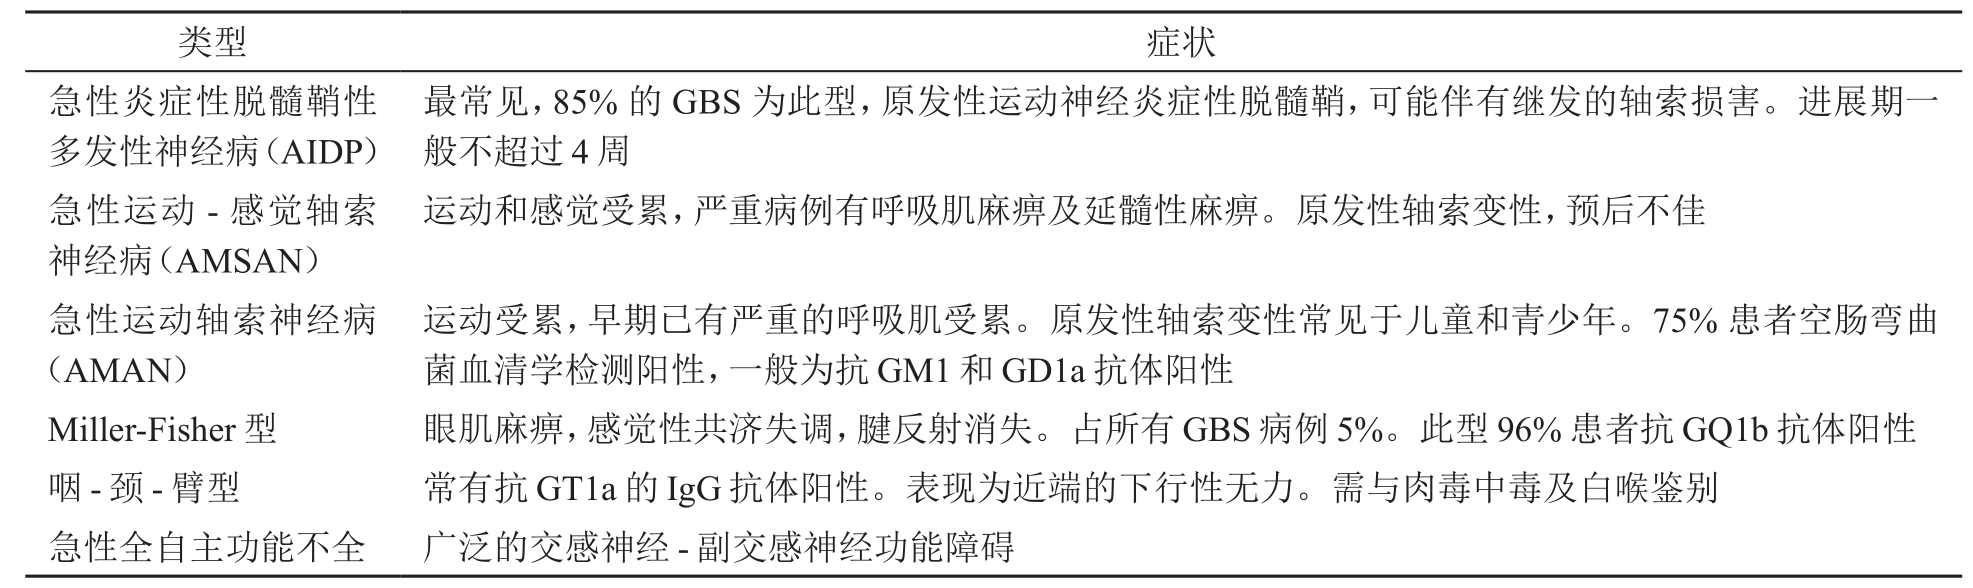
\includegraphics[width=6.57292in,height=1.94792in]{./images/Image00392.jpg}
\end{table}

\paragraph{心电图检查}

可见部分病例呈窦性心动过速、ST下降、T波低平或倒置、QT间期延长、房室传导阻滞、心肌劳损和心房纤颤。

\paragraph{肺功能测试}

最大吸气压和肺活量是非常重要的呼吸肌肉功能的测量内容,最大呼气压力也反映腹部肌肉的力量。严重患者需在床边呼吸状态监测,从而及时了解是否辅助通气。如肺活量下降至<
18ml/kg或动脉氧分压< 70mmHg则需行辅助通气。

\paragraph{影像学检查}

虽然非特异性,MRI可以显示神经根的影像增强。影像学脊柱CT或MRI扫描,有助于排除脊髓型颈椎病及其他疾病诊断。

\subsubsection{诊断注意事项}

根据患者急性或亚急性起病,病前1~3周有感染史,四肢对称性弛缓性瘫痪,末梢性感觉障碍伴脑神经受损,CSF示蛋白-细胞分离,肌电图早期F波或H反射延迟,诊断不难。但应注意与以下疾病鉴别:①脊髓灰质炎:起病时多有发热,出现肢体瘫痪,肢体瘫痪常局限于一侧下肢,无感觉障碍。②急性脊髓炎:发病前1~2周有发热病史,起病急,1~2天出现截瘫,受损平面以下运动障碍伴传导束性感觉障碍。早期出现尿便障碍,脑神经不受累。③低血钾型周期性瘫痪:迅速出现的四肢弛缓性瘫痪,无感觉障碍,呼吸肌、脑神经一般不受累。CSF正常,血钾降低,补钾治疗有效。④重症肌无力(MG):Fisher综合征注意与眼肌型MG、GBS与急性重症全身型MG等鉴别。MG受累骨骼肌病态疲劳、症状波动、晨轻暮重,新斯的明试验阳性等可助鉴别。

\subsubsection{诊断标准}

\paragraph{确立诊断条件}

有2项:①超过单肢的进行性无力;②腱反射减弱或消失。

\paragraph{强烈支持诊断的条件}

①病情进行性发展,数天至4周内停止进展;②症状相对对称;③感觉损害的症状或体征相对较轻;④脑神经受累,特别是双侧面肌无力;⑤自主神经功能障碍;⑥疼痛;⑦CSF中蛋白浓度升高;⑧典型电生理表现。

\paragraph{对诊断有疑问的条件}

①起病即出现严重的肺功能障碍,但肢体无力症状却较轻;②起病即出现严重的感觉体征,但无力症状却较轻;③起病时即有膀胱或直肠功能障碍;④发热起病;⑤明显的感觉平面;⑥疾病缓慢进展,无力症状较轻,无呼吸受累;⑦显著的持续性非对侧性无力;⑧持续性CSF单个核细胞增高(>
50 × 10\textsuperscript{6}
/L)或CSF中可见多形核细胞;⑨中枢神经系统受累。

\subsection{治疗}

\paragraph{治疗原则}

全身支持疗法,防止病情恶化;一旦发现呼吸肌麻痹,及时气管切开;应用免疫抑制疗法;预防肺部及泌尿系感染;早期开始康复治疗;降低死亡率和残疾率。

\paragraph{一般治疗及早期康复}

及早识别和处理焦虑症和抑郁症,以利于患者长期坚持治疗。急性期应嘱患者卧床休息,以减少疼痛刺激。饮食要富有营养并易于消化,防止肠道自主神经功能紊乱等消化道并发症。吞咽障碍者可取坐位鼻饲流质,以免误入气管窒息。便秘者可给缓泻剂,出现肠梗阻迹象应禁食,给予肠动力药。少数有尿潴留患者可加压按摩下腹部,无效时应及时导尿,并接上潮式引流装置。对瘫痪严重患者应防止足下垂及压疮,保持肢体功能位。穿长弹力袜预防深静脉血栓形成,小剂量肝素有助于预防肺栓塞。对呼吸肌麻痹者应行持续的心电监护,加强病情观察。应用广谱抗生素预防和治疗坠积性肺炎和脓毒血症。急性期后,即患者无明显疼痛时应开始早期康复治疗,防止肌肉萎缩。

\paragraph{呼吸肌麻痹的抢救}

\hypertarget{text00260.htmlux5cux23CHP8-8-3-3-1}{}
(1) 气管切开的时机:

对呼吸肌麻痹者应行气管切开,以利于气管内分泌物和CO\textsubscript{2}
排出,从而减少解剖学上的无效腔,便于辅助呼吸器的使用。应根据患者呼吸困难的程度,如呼吸频率、胸廓呼吸运动的幅度、血压、脉搏的情况决定气管切开的时机。当肺活量下降至正常的25\%~30\%,咳嗽无力,呼吸道分泌物排出困难,动脉血pH
7.3以下时,应及时气管切开,放置Y型管,以便吸痰和人工呼吸。

\hypertarget{text00260.htmlux5cux23CHP8-8-3-3-2}{}
(2) 呼吸机的应用:

对呼吸肌麻痹者采用人工呼吸机进行辅助呼吸,可防止CO\textsubscript{2}
麻醉及窒息的发生,一般认为应早期使用。目前普遍采用的正压通气的标准是:潮气量<
150~250ml;肺活量< 8~10ml/kg;血氧饱和度< 85\%;血氧分压<
60mmHg;CO\textsubscript{2} 分压>
50mmHg。使用呼吸机过程尚应密切观察患者的肺部情况,相应的监测和护理是抢救成功的关键。呼吸机的撤去应在患者的神经系统症状改善,呼吸功能恢复之后逐步进行。气管导管的拔出需待肺部感染得到控制,有力的咳嗽反射得到恢复,有24小时的自主正常呼吸功能方能进行。

\paragraph{免疫抑制治疗}

静脉注射免疫球蛋白和血浆置换疗法是治疗GBS的一线治疗,具体机制不详,但一般认为是由于消除外周血免疫活性细胞、细胞因子和抗体,从而减轻了神经损害,早期应用可缩短病程及减少辅助通气的花费。推荐单一使用,因联用并不增加疗效。

\hypertarget{text00260.htmlux5cux23CHP8-8-3-4-1}{}
(1) 静脉注射免疫球蛋白(intravenous immunoglobulin,IVIg):

IVIg应用方便,风险小,并发症相对较少,成为目前最受推崇的治疗方法。成人剂量0.4g/(kg•d),连用5天,尽早使用或在出现呼吸肌麻痹前使用。发热面红是常见的不良反应,减慢输液速度可减轻。临床试验比较IVIg、PE及二者合用的疗效无差异,推荐单一使用。禁忌证为先天性IgA缺乏,IVIg过敏史;相对禁忌证为严重的充血性心力衰竭和肾功能不全。

\hypertarget{text00260.htmlux5cux23CHP8-8-3-4-2}{}
(2) 血浆置换疗法(plasma exchange,PE):

直接去除血浆中致病因子如抗体。早期使用可缩短病程、改善预后、减少并发症。PE隔日进行1次,每次按50ml/kg体重或1~1.5倍的血浆容量计算,可用5\%白蛋白复原血容量,减少使用血浆的并发症。轻、中、重度患者应分别作2、4、6次。主要禁忌证是严重感染、心律失常、心功能不全及凝血系统疾病等。

\hypertarget{text00260.htmlux5cux23CHP8-8-3-4-3}{}
(3) 肾上腺皮质激素:

通常认为对GBS无效,并有不良反应,不推荐使用。无条件应用IVIg和PE的患者可考虑试用甲泼尼龙500mg/d或地塞米松10mg/d,静脉滴注,7~10天为一疗程。

\paragraph{抗生素}

考虑有胃肠道CJ感染者,可用大环内酯类抗生素治疗。如阿奇霉素0.5g/d、克拉霉素0.5~1.0g/d等。

AIDP具有自限性,预后好。瘫痪多在3周后开始恢复,大多数患者2个月~1年内恢复正常,约10\%患者遗留较严重后遗症。60岁以上、病情进展迅速并需要辅助呼吸、电生理检查示运动神经波幅降低是预后不良的危险因素。

\protect\hypertarget{text00261.html}{}{}

\hypertarget{text00261.htmlux5cux23CHP8-8-4}{}
参 考 文 献

1. Doorn PA,Kuitwaard K,Walgaard C,et al. IVIG treatment and
prognosis in Guillain-Barré syndrome. J Clin Immunol. 2010,30(Suppl
1):S74-78

2. Doorn PA. What's new in Guillain-Barré syndrome in 2007-2008?
Pharmacol Rep. J Peripher Nerv Syst,2009,14(2):72-74

3. Pithadia AB,Kakadia N. Guillain-Barré syndrome(GBS). Pharmacol
Rep,2010,62(2):220-332

4. Kaida K, Kusunoki S. Antibodies to gangliosides and ganglioside
complexes in Guillain-Barré syndrome and Fisher syndrome:mini-review. J
Neuroimmunol,2010,223(1-2):5-12.

5. Vucic S,Kiernan MC,Cornblath DR. Guillain-Barré syndrome:an
update. J Clin Neurosci,2009,16(6):733-741

6. Doorn PA,Ruts L,Jacobs BC. Clinical features,pathogenesis,and
treatment of Guillain-Barré syndrome. Lancet
Neurol,2008,7(10):939-950

\protect\hypertarget{text00262.html}{}{}

\chapter{周期性瘫痪}

周期性瘫痪(periodic
paralysis,PP)是一组反复发作的骨骼肌弛缓性瘫痪为特征的肌病,与钾代谢异常有关。肌无力可持续数小时或数周,发作间歇期完全正常,根据发病时血清钾的改变,可分为低血钾型、高血钾型和正常血钾型三类,其中以低血钾型周期性瘫痪(hypokalemic
PP,HoPP)最常见。由甲状腺功能亢进、醛固酮增多症、肾衰竭和代谢性疾病所致低钾而瘫痪者称为继发性周期性瘫痪。

\subsection{病因与发病机制}

周期性瘫痪属于离子通道病(ion channel
disease)。离子通道病是由离子通道功能异常引起的一组疾病,主要侵犯神经和肌肉系统,也可累及心脏和肾脏等。周期性瘫痪是1991年Ptacek首先提出的第一个离子通道病。离子通道疾病包括中枢神经系统通道病和骨骼肌钙通道病,HoPP属于后者。

HoPP为常染色体显性遗传性疾病,其致病基因主要位于1号染色体长臂(1q\textsuperscript{31-32}
),该基因编码肌细胞二氢吡啶敏感的L型钙离子通道蛋白,是二氢吡啶复合受体的一部分,位于横管系统,通过调控肌质网钙离子的释放而影响肌肉的兴奋-收缩偶联。肌无力在饱餐后或激烈活动后的休息中最易发作,能促使钾离子传入细胞内的因素如注射胰岛素、肾上腺素或大量葡萄糖也能诱发。其发病机制可能与骨骼肌细胞膜内、外钾离子浓度的波动有关。正常情况下,钾离子浓度在肌膜内高,肌膜外低,当两侧保持正常比例时,肌膜才能维持正常的静息电位,才能为乙酰胆碱(ACh)的去极化产生正常的反应。本病患者的肌细胞膜经常处于轻度去极化状态,较不稳定,电位稍有变化即产生钠离子在膜上的通路受阻,导致电活动的传播障碍。在疾病发作期间,受累肌肉对一切电刺激均不起反应,处于瘫痪状态。

高血钾型和正常血钾型周期性瘫痪属于骨骼肌钠通道病,致病基因位于第17号染色体长臂(17q\textsuperscript{13}
),由于编码骨骼肌门控钠通道蛋白的α-亚单位基因的点突变,导致氨基酸的改变,引起肌细胞膜钠离子通道功能异常,膜对钠的通透性增加或肌细胞内钾、钠转换能力缺陷,钠内流增加,钾离子从细胞内转移到细胞外,膜不能正常复极呈持续去极化,肌细胞膜正常兴奋性消失,产生肌无力。

\subsection{诊断}

\subsubsection{低血钾型周期性瘫痪}

是在1863年由Gavare首先描述的。1885年Goldflam强调此病与遗传有关,故又称家族性遗传性周期性瘫痪。目前认为HoPP是常染色体显性遗传钙通道病,国外病例常有家族史,国内则多为散发病例。部分HoPP病例与甲状腺功能亢进有关,称为甲亢性周期性瘫痪。

\paragraph{临床表现特点}

任何年龄均可发病,但以20~40岁青壮年多见,随年龄增长发作次数减少。其临床特点是:①发病诱因包括饱餐(尤其过量进食碳水化合物)、酗酒、过度劳累、剧烈运动、寒冷、感染、创伤、情绪激动、焦虑和月经,以及注射胰岛素、肾上腺素、皮质激素或大量输入葡萄糖等。②发作前可有肢体酸胀、疼痛、麻木、烦渴、多汗、面色潮红、嗜睡、恶心和恐惧等前驱症状,此时努力进行活动可能使其发作顿挫。③常于凌晨或半夜熟睡醒来时突然发现肢体无力,日间清醒发病者仅少数。无力常始于下肢,一般双侧对称,但亦可为一组或一侧较重,在数小时内波及上肢、躯干,均为弛缓性瘫痪。瘫痪以肢体为主,近端重于远端,下肢重于上肢,常在数小时(1~2小时)至1~2天内到达高峰。瘫痪肢体肌张力降低,腱反射减弱或消失。颈项以上脊髓肌和脑神经支配肌肉一般不受累及,膀胱直肠括约肌功能也很少受累。少数严重病例可发生呼吸肌麻痹、尿便潴留、心动过速或过缓、心律失常、血压下降等情况甚至危及生命。④发作时神志始终清醒,瘫痪肢体可有轻度肿胀,触摸时有坚实感,患肢可有疼痛和感觉异常,但客观感觉无障碍,深、浅感觉均正常。⑤发作期间,可伴有自主神经功能障碍,表现为口干、皮肤苍白、心率减慢、心律不齐、血压升高或下降等,偶有膀胱及直肠功能的障碍。⑥每次发作持续数小时或1~2天就可自行恢复,个别病例长达1周。恢复颇为迅速,仅1~2小时,最先发作的肌群常最早恢复,开始恢复后的肢体被动运动可加速肌力改善。部分患者在肌肉恢复时伴多尿、大汗及瘫痪的肌肉酸痛和僵硬。⑦发作频率因人而异,相差悬殊,数周或数月一次,个别病例发作频繁,甚至每天都发作;也有数年发作一次或终生仅发作一次者。一般年轻时发作较频,成年后逐渐减少,50岁以后常不再发作。少数患者在患病多年后发生主要影响肢带肌群的缓慢进行性肌病。

\paragraph{辅助检查}

①发作时血清钾降低至3.5mmol/L以下,可低至1~2mmol/L,尿钾也减少,血钠可升高。间歇期正常。②心电图检查呈典型低血钾性改变:P-R间期和Q-T间期延长,QRS增宽,ST段降低,T波低平和U波出现。③肌电图示运动电位时限短、波幅低,完全瘫痪时运动单位电位消失,电刺激无反应,膜静息电位低于正常。

\paragraph{诊断注意事项}

根据典型的呈周期性发作的短时期的下运动神经元瘫痪,无意识障碍和感觉障碍,即应考虑本病的诊断。急行血钾和心电图检查有助于明确诊断。应注意与以下疾病鉴别:①Guillain-Barre综合征:本病呈四肢弛缓性瘫痪,远端重于近端,可有周围性感觉障碍和脑神经损害,脑脊液蛋白-细胞分离现象,肌电图神经源性损害。此外,起病不如HoPP之急,病程至少数周而不可能在数小时或1~2天内恢复。②重症肌无力:亚急性起病,可累及四肢及脑神经支配肌肉,症状呈波动性,晨轻暮重,病态疲劳。疲劳试验及新斯的明试验阳性。血清钾正常,重复神经电刺激波幅递减,抗Ach受体抗体阳性可资鉴别。③继发性低血钾:散发病例应与可反复引起低血钾的疾病鉴别,如原发性醛固酮增多症、肾小管酸中毒、甲状腺功能亢进、失钾性肾炎、腹泻、运用利尿剂后等也可出现低钾性瘫痪,但均有原发病的其他特征可供诊断参考。④癔症性瘫痪无腱反射或肌肉电反应性的改变。⑤肌红蛋白尿症也可表现为发作性的急性下运动神经元瘫痪,在几天内恢复,但伴明显的全身症状和肌肉疼痛,尿呈特殊的棕红色。⑥急性钡中毒可引起四肢瘫痪、眼睑下垂、发音及吞咽困难,在我国四川常见。⑦高血钾型、正常血钾型周期性瘫痪(见下述)。

\subsubsection{高血钾型周期性瘫痪}

高血钾型周期性瘫痪(hyperkalemic
PP,HyPP)又称强直性周期性瘫痪、遗传性发作性无力症(adynamia episodica
hereditaria),较少见。1951年由Tyler首先报道,呈常染色体显性遗传。多见于北欧国家。临床特点是:①多在10岁前起病,男性居多,饥饿、寒冷、剧烈活动后休息、钾盐摄入等可以诱发,进食或坚持轻度的体力活动可使该次发作顿挫或推迟。②常在白天运动后休息20~30分钟后发病,其前驱症状与瘫痪经过与HoPP相似,但血清钾变化正好相反,症状出现于血清钾高于正常时。但肌无力程度与血钾水平不相平行。瘫痪程度一般较轻,严重者累及颈肌和眼外肌。多伴有肌肉的痛性痉挛。③常见有不引起自觉症状的轻度肌强直现象(如进食冷饮后发音不清,手浸于冷水中稍长时间后动作僵拙不灵,叩击舌肌时发生局部强直性收缩而引起凹陷)。④发作通常为时短暂,持续15~60分钟,一般在30分钟~24小时内恢复,偶有持续1~2天以上者。发作频率因人而异,每日至每年发作数次。30岁以后发作逐渐终止。一些反复发作的患者可遗有永久肌无力。⑤辅助检查:发作时血清钾增高,血清酶如肌酸激酶(CK)可正常或升高,心电图呈高血钾性改变,如T波高尖、P波降低甚至消失、QRS波改变等。

根据常染色体显性遗传家族史,儿童发作性无力伴肌强直,无感觉障碍和高级神经活动异常,血钾增高,可作出诊断。应注意与低血钾型、正常血钾型周期性瘫痪和先天性副肌强直症鉴别,还应注意与继发性高血钾瘫痪鉴别,如肾功能衰竭、肾上腺皮质功能不全、醛固酮缺乏症和药物性高血钾等。

诊断HyPP有困难时,可作以下诱发试验:①钾负荷试验:即口服钾以观察可否诱发肌无力。方法是口服4~5g氯化钾,如为本病患者,服后30~90分钟内出现肌无力,数分钟至1小时达高峰,持续20分钟~1天。应注意在患者心、肾功能、血钾水平正常并在心电监护下进行。②运动诱发试验:让患者蹬自行车,该车加有400~750kg阻力,连续30~60分钟,停车后30分钟如诱发肌无力伴血钾升高可诊断本病。③冷水诱发试验:将前臂浸入11~13℃水中,如为本病患者,20~30分钟可以诱发肌无力,停止浸冷水10分钟后可恢复。

\subsubsection{正常血钾型周期性瘫痪}

正常血钾型周期性瘫痪(normal kalemic
PP)又名钠反应性正常血钾型周期性瘫痪。为常染色体显性遗传,本型罕见。多在10岁以前发病,常在夜间睡后或清晨醒转时发生四肢瘫痪,或仅选择性地影响某些肌肉(如小腿肌、肩臂肌),但呼吸肌和吞咽肌极少受累。发作持续时间较长,数日至数周,多数在10天以上,约每1~3个月发作一次。运动后休息、寒冷、限制钠盐摄入或补充钾盐均可诱发,补钠后好转。发作时血、尿中钾正常,而尿钠含量增高。部分患者平日极度嗜盐。主要应与Guillain-Barre综合征、低血钾型与高血钾型周期性瘫痪鉴别。

\subsection{治疗}

\paragraph{低血钾型周期性瘫痪}

发作时应立即补钾,如果不伴呕吐,原则上以口服氯化钾(10g/d)为主,成人一次顿服4~5g,以后每次1~2g,每日3~4次,完全恢复后改为每次1g,每日3次,维持1~2周。为减轻对胃肠道的刺激,可与牛奶或橘子汁混合口服。严重者需静脉补钾,可用10\%氯化钾30~40ml加入0.9\%氯化钠液或林格液1000ml中静滴,待症状缓解后改为口服氯化钾。上述补钾过程应有血清钾和心电图监测。严重患者出现呼吸肌麻痹时应予辅助呼吸,严重心律失常者应及时纠正。为加强补钾效果,可辅用镁剂治疗,如25\%硫酸镁10ml加入上述液体中静滴。不完全性瘫痪可鼓励患者自主活动以加速恢复。经常发作的病例,应避免疲劳、受冷、酗酒和饱餐大量碳水化合物等诱发因素,平时多食榨菜、芹菜、橘子等含钾蔬菜水果。也可口服氯化钾0.5g,每天3次;或乙酰唑胺0.25g,每天1~4次;或螺内酯20~40mg,每天2~4次,可预防发病。低钠高钾、低碳水化合物饮食可能有助于减少发作。甲亢性HoPP患者,在对甲亢进行适当的治疗后常可终止发作或显著减轻。

\paragraph{高血钾型周期性瘫痪}

由于每次发作轻、时间短,大多无需特殊处理。病情较重者,可用10\%葡萄糖酸钙或氯化钙10~20ml加入25\%~50\%葡萄糖液40~60ml中缓慢静脉注射,也可静滴10\%葡萄糖液500ml加正规胰岛素10~20u,以促进细胞内糖原的合成和K\textsuperscript{+}
自细胞外液进入细胞内液;或静脉注射呋塞米20~40mg利尿排钾,也可静滴碱剂如5\%碳酸氢钠。发作频繁者,于发作间歇期给高碳水化合物饮食,口服氢氯噻嗪25mg,每天2~3次,可预防发作。

\paragraph{正常血钾型周期性瘫痪}

发作时可用大剂量0.9\%氯化钠液静滴使瘫痪好转。同时可给予:①钙剂:10\%葡萄糖酸钙10ml静脉注射,每天1~2次;或用钙片0.6~1.2g/d口服;②乙酰唑胺0.25g口服,每天2~4次;或用氟氢可的松0.1~0.2mg/d;③每日口服10~15g食盐。避免进食含钾多的食物,如肉类、香蕉、菠菜、薯类等。

\protect\hypertarget{text00263.html}{}{}

\hypertarget{text00263.htmlux5cux23CHP8-9-4}{}
参 考 文 献

1. 贾建平.神经病学.第6版.北京:人民卫生出版社,2008: 365-368

2. Cannon SC. An expanding view for the molecular basis of familial
periodic paralysis. Neuromuscul Dis,2002,12(6):533

3. 张文武 .急诊内科学.第2版.北京:人民卫生出版社,2007

\protect\hypertarget{text00264.html}{}{}

